\documentclass[final]{book}
\newcommand{\doctitle}{HSA Runtime Programmer's Reference Manual}
\newcommand{\docversion}{0.187}

\usepackage[T1]{fontenc}

\usepackage[top=2.5cm,bottom=2.5cm,left=2.5cm,right=2.5cm]{geometry}

\usepackage[toc,page]{appendix}
\usepackage[usenames,dvipsnames,svgnames,table]{xcolor}
  \definecolor{lightgray}{gray}{0.94}
\usepackage{makeidx}
\usepackage[final]{graphicx}
\usepackage{pbox}
\usepackage{sidecap}
\usepackage{float}

\usepackage[final]{listings}

\usepackage{longtable}

\usepackage{tikz}
\usetikzlibrary{arrows,automata,positioning,chains}
\tikzset{
        >=angle 45}

\usepackage{calc}
\catcode`\_=12

\usepackage{ifthen}
\usepackage{textcomp}

\usepackage{paralist}

\usepackage{fancyhdr}

\usepackage{imakeidx}
\makeindex[name=api,title=Index - Core APIs,columns=1,intoc]
\makeindex[name=ext,title=Index - Extension APIs,columns=1,intoc]

\usepackage{times}

\usepackage{enumitem}

\lstset{        backgroundcolor=\color{lightgray},
        basicstyle=\footnotesize,
        breakatwhitespace=true,
        breaklines=true,
        captionpos=b,              columns=fullflexible,
        commentstyle=\color{ForestGreen},
        emphstyle={\textbf},
        frame=single,
        framexbottommargin=3pt,         framextopmargin=3pt,         inputencoding=utf8,
        keywordstyle=\color{blue},
        language=C,
        rulecolor=\color{lightgray},         showstringspaces=false,
        tabsize=4,
}
\renewcommand{\lstlistingname}{Example}
\renewcommand{\lstlistlistingname}{List of \lstlistingname s}
\makeatletter{}\lstset{emph={hsa_status_string,hsa_init,hsa_shut_down,hsa_system_get_info,hsa_agent_get_info,hsa_iterate_agents,hsa_signal_create,hsa_signal_destroy,hsa_signal_load_acquire,hsa_signal_load_relaxed,hsa_signal_store_relaxed,hsa_signal_store_release,hsa_signal_exchange_acq_rel,hsa_signal_exchange_acquire,hsa_signal_exchange_relaxed,hsa_signal_exchange_release,hsa_signal_cas_acq_rel,hsa_signal_cas_acquire,hsa_signal_cas_relaxed,hsa_signal_cas_release,hsa_signal_add_acq_rel,hsa_signal_add_acquire,hsa_signal_add_relaxed,hsa_signal_add_release,hsa_signal_subtract_acq_rel,hsa_signal_subtract_acquire,hsa_signal_subtract_relaxed,hsa_signal_subtract_release,hsa_signal_and_acq_rel,hsa_signal_and_acquire,hsa_signal_and_relaxed,hsa_signal_and_release,hsa_signal_or_acq_rel,hsa_signal_or_acquire,hsa_signal_or_relaxed,hsa_signal_or_release,hsa_signal_xor_acq_rel,hsa_signal_xor_acquire,hsa_signal_xor_relaxed,hsa_signal_xor_release,hsa_signal_wait_acquire,hsa_signal_wait_relaxed,hsa_queue_create,hsa_queue_destroy,hsa_queue_inactivate,hsa_queue_load_read_index_acquire,hsa_queue_load_read_index_relaxed,hsa_queue_load_write_index_acquire,hsa_queue_load_write_index_relaxed,hsa_queue_store_write_index_relaxed,hsa_queue_store_write_index_release,hsa_queue_cas_write_index_acq_rel,hsa_queue_cas_write_index_acquire,hsa_queue_cas_write_index_relaxed,hsa_queue_cas_write_index_release,hsa_queue_add_write_index_acq_rel,hsa_queue_add_write_index_acquire,hsa_queue_add_write_index_relaxed,hsa_queue_add_write_index_release,hsa_queue_store_read_index_relaxed,hsa_queue_store_read_index_release,hsa_region_get_info,hsa_agent_iterate_regions,hsa_memory_allocate,hsa_memory_free,hsa_memory_register,hsa_memory_deregister,hsa_vendor_extension_query,hsa_extension_query,hsa_ext_finalize,hsa_ext_query_finalization_code_descriptor_count,hsa_ext_query_finalization_code_descriptor,hsa_ext_destroy_finalization,hsa_ext_serialize_finalization,hsa_ext_deserialize_finalization,hsa_ext_program_create,hsa_ext_program_destroy,hsa_ext_add_module,hsa_ext_finalize_program,hsa_ext_query_program_agent_id,hsa_ext_query_program_agent_count,hsa_ext_query_program_agents,hsa_ext_query_program_module_count,hsa_ext_query_program_modules,hsa_ext_query_program_brig_module,hsa_ext_query_call_convention,hsa_ext_query_symbol_definition,hsa_ext_define_program_allocation_global_variable_address,hsa_ext_query_program_allocation_global_variable_address,hsa_ext_define_agent_allocation_global_variable_address,hsa_ext_query_agent_global_variable_address,hsa_ext_define_readonly_variable_address,hsa_ext_query_readonly_variable_address,hsa_ext_query_kernel_descriptor_address,hsa_ext_query_indirect_function_descriptor_address,hsa_ext_validate_program,hsa_ext_validate_program_module,hsa_ext_serialize_program,hsa_ext_deserialize_program,hsa_ext_image_get_format_capability,hsa_ext_image_get_info,hsa_ext_image_create_handle,hsa_ext_image_import,hsa_ext_image_export,hsa_ext_image_copy,hsa_ext_image_clear,hsa_ext_image_destroy_handle,hsa_ext_sampler_create_handle,hsa_ext_sampler_destroy_handle,}} 

\newcommand{\hsaarg}[1]{\textit{#1}}
\newcommand{\reffun}[1]{\textbf{#1}}
\newcommand{\refarg}[1]{\textit{#1}}
\newcommand{\reffld}[1]{\textit{#1}}
\newcommand{\reftyp}[1]{#1}
\newcommand{\refenu}[1]{\reftyp{#1}}
\newcommand{\refhsl}[1]{\reffun{#1}}

\usepackage{pdftexcmds}
\makeatletter{}\makeatletter
\newcommand{\hsaref}[1]{\ifnum\pdf@strcmp{#1}{blablablablabla}=0 blablablablabla
\else\ifnum\pdf@strcmp{#1}{HSA_STATUS_SUCCESS}=0\hyperlink{group__status_1ggad755322e7ff95456520e8abdbe90d225ae382ea0c9c05cce5a60d0317375159cc}{\refenu{HSA_\-STATUS_\-SUCCESS}}\else\ifnum\pdf@strcmp{#1}{HSA_STATUS_INFO_BREAK}=0\hyperlink{group__status_1ggad755322e7ff95456520e8abdbe90d225a86c476121ca787ff75f6a4676507b221}{\refenu{HSA_\-STATUS_\-INFO_\-BREAK}}\else\ifnum\pdf@strcmp{#1}{HSA_EXT_STATUS_INFO_ALREADY_INITIALIZED}=0\hyperlink{group__status_1ggad755322e7ff95456520e8abdbe90d225a0882e3ebb9cc8a5c6033c43ee7a6d898}{\refenu{HSA_\-EXT_\-STATUS_\-INFO_\-ALREADY_\-INITIALIZED}}\else\ifnum\pdf@strcmp{#1}{HSA_EXT_STATUS_INFO_UNRECOGNIZED_OPTIONS}=0\hyperlink{group__status_1ggad755322e7ff95456520e8abdbe90d225a60343279bea68766b037297915b5f903}{\refenu{HSA_\-EXT_\-STATUS_\-INFO_\-UNRECOGNIZED_\-OPTIONS}}\else\ifnum\pdf@strcmp{#1}{HSA_STATUS_ERROR}=0\hyperlink{group__status_1ggad755322e7ff95456520e8abdbe90d225a60edf4d82e4703ff750ea38d619fea88}{\refenu{HSA_\-STATUS_\-ERROR}}\else\ifnum\pdf@strcmp{#1}{HSA_STATUS_ERROR_INVALID_ARGUMENT}=0\hyperlink{group__status_1ggad755322e7ff95456520e8abdbe90d225ac7d3651f75107d2a6a8ba3b25683c030}{\refenu{HSA_\-STATUS_\-ERROR_\-INVALID_\-ARGUMENT}}\else\ifnum\pdf@strcmp{#1}{HSA_STATUS_ERROR_INVALID_QUEUE_CREATION}=0\hyperlink{group__status_1ggad755322e7ff95456520e8abdbe90d225a7b27f50e23a776b496b8b4707f21ccad}{\refenu{HSA_\-STATUS_\-ERROR_\-INVALID_\-QUEUE_\-CREATION}}\else\ifnum\pdf@strcmp{#1}{HSA_STATUS_ERROR_INVALID_ALLOCATION}=0\hyperlink{group__status_1ggad755322e7ff95456520e8abdbe90d225ac818189ff640d38ce13558e72daddb75}{\refenu{HSA_\-STATUS_\-ERROR_\-INVALID_\-ALLOCATION}}\else\ifnum\pdf@strcmp{#1}{HSA_STATUS_ERROR_INVALID_AGENT}=0\hyperlink{group__status_1ggad755322e7ff95456520e8abdbe90d225a3a5d835c109c2d0ad5b9c2771e133e5d}{\refenu{HSA_\-STATUS_\-ERROR_\-INVALID_\-AGENT}}\else\ifnum\pdf@strcmp{#1}{HSA_STATUS_ERROR_INVALID_REGION}=0\hyperlink{group__status_1ggad755322e7ff95456520e8abdbe90d225ad63594ac02edec7ae7aa7722c11afcd9}{\refenu{HSA_\-STATUS_\-ERROR_\-INVALID_\-REGION}}\else\ifnum\pdf@strcmp{#1}{HSA_STATUS_ERROR_INVALID_SIGNAL}=0\hyperlink{group__status_1ggad755322e7ff95456520e8abdbe90d225a7b4c8c0d4c99a1fe966abc2d39b575fe}{\refenu{HSA_\-STATUS_\-ERROR_\-INVALID_\-SIGNAL}}\else\ifnum\pdf@strcmp{#1}{HSA_STATUS_ERROR_INVALID_QUEUE}=0\hyperlink{group__status_1ggad755322e7ff95456520e8abdbe90d225aa3c762eb6a61b358702b45259d1686c4}{\refenu{HSA_\-STATUS_\-ERROR_\-INVALID_\-QUEUE}}\else\ifnum\pdf@strcmp{#1}{HSA_STATUS_ERROR_OUT_OF_RESOURCES}=0\hyperlink{group__status_1ggad755322e7ff95456520e8abdbe90d225a1a77fcf36d0d140874c4361ab093eff7}{\refenu{HSA_\-STATUS_\-ERROR_\-OUT_\-OF_\-RESOURCES}}\else\ifnum\pdf@strcmp{#1}{HSA_STATUS_ERROR_INVALID_PACKET_FORMAT}=0\hyperlink{group__status_1ggad755322e7ff95456520e8abdbe90d225a3fad45f72111eb99de5d8daef26c372c}{\refenu{HSA_\-STATUS_\-ERROR_\-INVALID_\-PACKET_\-FORMAT}}\else\ifnum\pdf@strcmp{#1}{HSA_STATUS_ERROR_RESOURCE_FREE}=0\hyperlink{group__status_1ggad755322e7ff95456520e8abdbe90d225a6406af88203fcbec4179fbb71cc66b65}{\refenu{HSA_\-STATUS_\-ERROR_\-RESOURCE_\-FREE}}\else\ifnum\pdf@strcmp{#1}{HSA_STATUS_ERROR_NOT_INITIALIZED}=0\hyperlink{group__status_1ggad755322e7ff95456520e8abdbe90d225a34ea59ade5bfce95eee935238a99f5b5}{\refenu{HSA_\-STATUS_\-ERROR_\-NOT_\-INITIALIZED}}\else\ifnum\pdf@strcmp{#1}{HSA_STATUS_ERROR_REFCOUNT_OVERFLOW}=0\hyperlink{group__status_1ggad755322e7ff95456520e8abdbe90d225aa9218eed04d1d2ffc5ed8f33f2cd1c9b}{\refenu{HSA_\-STATUS_\-ERROR_\-REFCOUNT_\-OVERFLOW}}\else\ifnum\pdf@strcmp{#1}{HSA_EXT_STATUS_ERROR_DIRECTIVE_MISMATCH}=0\hyperlink{group__status_1ggad755322e7ff95456520e8abdbe90d225ae16bcc443d027a0b880fd58f0443227b}{\refenu{HSA_\-EXT_\-STATUS_\-ERROR_\-DIRECTIVE_\-MISMATCH}}\else\ifnum\pdf@strcmp{#1}{HSA_EXT_STATUS_ERROR_IMAGE_FORMAT_UNSUPPORTED}=0\hyperlink{group__status_1ggad755322e7ff95456520e8abdbe90d225a42108181943a2d94749d95dc7942b7d0}{\refenu{HSA_\-EXT_\-STATUS_\-ERROR_\-IMAGE_\-FORMAT_\-UNSUPPORTED}}\else\ifnum\pdf@strcmp{#1}{HSA_EXT_STATUS_ERROR_IMAGE_SIZE_UNSUPPORTED}=0\hyperlink{group__status_1ggad755322e7ff95456520e8abdbe90d225a3ff898da367040b1f382c14c9f0a1bab}{\refenu{HSA_\-EXT_\-STATUS_\-ERROR_\-IMAGE_\-SIZE_\-UNSUPPORTED}}\else\ifnum\pdf@strcmp{#1}{hsa_status_t}=0\hyperlink{group__status_1gad755322e7ff95456520e8abdbe90d225}{\reftyp{hsa_\-status_\-t}}\else\ifnum\pdf@strcmp{#1}{hsa_status_string}=0\hyperlink{group__status_1gad3c84c6119c06322ee8e9cd44fa47b25}{\reffun{hsa_\-status_\-string}}\else\ifnum\pdf@strcmp{#1}{hsa_powertwo8_t}=0\hyperlink{group__common_1ga143c7c845aca213614c1d79b65c35a0c}{\reftyp{hsa_\-powertwo8_\-t}}\else\ifnum\pdf@strcmp{#1}{HSA_POWERTWO_1}=0\hyperlink{group__common_1gga45e8c4edc00ad0dc2c9e6e14e8610977a13bfa83a83c0f555efe4bbcca6b9cddf}{\refenu{HSA_\-POWERTWO_\-1}}\else\ifnum\pdf@strcmp{#1}{HSA_POWERTWO_2}=0\hyperlink{group__common_1gga45e8c4edc00ad0dc2c9e6e14e8610977a465003dadda71ae8589097dd03202daf}{\refenu{HSA_\-POWERTWO_\-2}}\else\ifnum\pdf@strcmp{#1}{HSA_POWERTWO_4}=0\hyperlink{group__common_1gga45e8c4edc00ad0dc2c9e6e14e8610977a04e128660c6aee9bd09b8be8683a4df9}{\refenu{HSA_\-POWERTWO_\-4}}\else\ifnum\pdf@strcmp{#1}{HSA_POWERTWO_8}=0\hyperlink{group__common_1gga45e8c4edc00ad0dc2c9e6e14e8610977a6b602015c0db012f426e22c0354fbd05}{\refenu{HSA_\-POWERTWO_\-8}}\else\ifnum\pdf@strcmp{#1}{HSA_POWERTWO_16}=0\hyperlink{group__common_1gga45e8c4edc00ad0dc2c9e6e14e8610977abc59007bbaea149704bb50a1aa70b7aa}{\refenu{HSA_\-POWERTWO_\-16}}\else\ifnum\pdf@strcmp{#1}{HSA_POWERTWO_32}=0\hyperlink{group__common_1gga45e8c4edc00ad0dc2c9e6e14e8610977af13ebd4aecb93fd78bee555d26ed62a7}{\refenu{HSA_\-POWERTWO_\-32}}\else\ifnum\pdf@strcmp{#1}{HSA_POWERTWO_64}=0\hyperlink{group__common_1gga45e8c4edc00ad0dc2c9e6e14e8610977a93252b7ad8bdcbec33390212e8897bd5}{\refenu{HSA_\-POWERTWO_\-64}}\else\ifnum\pdf@strcmp{#1}{HSA_POWERTWO_128}=0\hyperlink{group__common_1gga45e8c4edc00ad0dc2c9e6e14e8610977ae78a1c50ad98ae134e34186acd52174e}{\refenu{HSA_\-POWERTWO_\-128}}\else\ifnum\pdf@strcmp{#1}{HSA_POWERTWO_256}=0\hyperlink{group__common_1gga45e8c4edc00ad0dc2c9e6e14e8610977ae774bb9d85b5f7f9968ab76e50c23a6b}{\refenu{HSA_\-POWERTWO_\-256}}\else\ifnum\pdf@strcmp{#1}{hsa_powertwo_t}=0\hyperlink{group__common_1ga45e8c4edc00ad0dc2c9e6e14e8610977}{\reftyp{hsa_\-powertwo_\-t}}\else\ifnum\pdf@strcmp{#1}{hsa_dim3_t}=0\hyperlink{group__common_1ga6f7883588491965c45382cd996351aa2}{\reftyp{hsa_\-dim3_\-t}}\else\ifnum\pdf@strcmp{#1}{HSA_DIM_X}=0\hyperlink{group__common_1ggaa7eb83c51012a3b6f016f7b3388964efa5a172a4cf084b71b9bafd68eaf159efc}{\refenu{HSA_\-DIM_\-X}}\else\ifnum\pdf@strcmp{#1}{HSA_DIM_Y}=0\hyperlink{group__common_1ggaa7eb83c51012a3b6f016f7b3388964efa863557e1bf7f7ba4f7ac00527f214d0e}{\refenu{HSA_\-DIM_\-Y}}\else\ifnum\pdf@strcmp{#1}{HSA_DIM_Z}=0\hyperlink{group__common_1ggaa7eb83c51012a3b6f016f7b3388964efaa2ea7a7aba09bb743508177f196d2983}{\refenu{HSA_\-DIM_\-Z}}\else\ifnum\pdf@strcmp{#1}{hsa_dim_t}=0\hyperlink{group__common_1gaa7eb83c51012a3b6f016f7b3388964ef}{\reftyp{hsa_\-dim_\-t}}\else\ifnum\pdf@strcmp{#1}{hsa_runtime_caller_t}=0\hyperlink{group__common_1ga7d9b1191602415f5dd3893985cc93826}{\reftyp{hsa_\-runtime_\-caller_\-t}}\else\ifnum\pdf@strcmp{#1}{hsa_runtime_alloc_data_callback_t}=0\hyperlink{group__common_1ga30804c05fe32b4ab9da480280dba8cc5}{\reftyp{hsa_\-runtime_\-alloc_\-data_\-callback_\-t}}\else\ifnum\pdf@strcmp{#1}{hsa_init}=0\hyperlink{group__initshutdown_1ga5b8574433e7dbcbd31ea397a02e3c32b}{\reffun{hsa_\-init}}\else\ifnum\pdf@strcmp{#1}{hsa_shut_down}=0\hyperlink{group__initshutdown_1ga97bdbccbd372609ad14a7ae7389cf4bf}{\reffun{hsa_\-shut_\-down}}\else\ifnum\pdf@strcmp{#1}{HSA_SYSTEM_INFO_VERSION_MAJOR}=0\hyperlink{group__agentinfo_1gga5358716e320ad8a78b78ef44d8783b0bac33519a29a9fa32f1dd179b9f8af8243}{\refenu{HSA_\-SYSTEM_\-INFO_\-VERSION_\-MAJOR}}\else\ifnum\pdf@strcmp{#1}{HSA_SYSTEM_INFO_VERSION_MINOR}=0\hyperlink{group__agentinfo_1gga5358716e320ad8a78b78ef44d8783b0ba0ac419f557187a4cfcdeb604f37bb4ae}{\refenu{HSA_\-SYSTEM_\-INFO_\-VERSION_\-MINOR}}\else\ifnum\pdf@strcmp{#1}{HSA_SYSTEM_INFO_TIMESTAMP}=0\hyperlink{group__agentinfo_1gga5358716e320ad8a78b78ef44d8783b0bac9043678e4c1dd887fcf71cabee228f6}{\refenu{HSA_\-SYSTEM_\-INFO_\-TIMESTAMP}}\else\ifnum\pdf@strcmp{#1}{HSA_SYSTEM_INFO_TIMESTAMP_FREQUENCY}=0\hyperlink{group__agentinfo_1gga5358716e320ad8a78b78ef44d8783b0bae2a8bb2c1322968a95b8ed49c34d54f5}{\refenu{HSA_\-SYSTEM_\-INFO_\-TIMESTAMP_\-FREQUENCY}}\else\ifnum\pdf@strcmp{#1}{HSA_SYSTEM_INFO_SIGNAL_MAX_WAIT}=0\hyperlink{group__agentinfo_1gga5358716e320ad8a78b78ef44d8783b0ba851f3f7745ed5524352598d2a0f02e9a}{\refenu{HSA_\-SYSTEM_\-INFO_\-SIGNAL_\-MAX_\-WAIT}}\else\ifnum\pdf@strcmp{#1}{hsa_system_info_t}=0\hyperlink{group__agentinfo_1ga5358716e320ad8a78b78ef44d8783b0b}{\reftyp{hsa_\-system_\-info_\-t}}\else\ifnum\pdf@strcmp{#1}{hsa_system_get_info}=0\hyperlink{group__agentinfo_1gaab2916fb980fbafdcea712ba6a99d46d}{\reffun{hsa_\-system_\-get_\-info}}\else\ifnum\pdf@strcmp{#1}{hsa_agent_t}=0\hyperlink{group__agentinfo_1ga27393931438432bb42772bc10f5d4941}{\reftyp{hsa_\-agent_\-t}}\else\ifnum\pdf@strcmp{#1}{HSA_AGENT_FEATURE_DISPATCH}=0\hyperlink{group__agentinfo_1ggadf226614ab6da93b301f100cfd58e504adbf09dd5c243aaa6ff5abd70168cd837}{\refenu{HSA_\-AGENT_\-FEATURE_\-DISPATCH}}\else\ifnum\pdf@strcmp{#1}{HSA_AGENT_FEATURE_AGENT_DISPATCH}=0\hyperlink{group__agentinfo_1ggadf226614ab6da93b301f100cfd58e504a12b2ba8c7b09e76817346b74152dbfae}{\refenu{HSA_\-AGENT_\-FEATURE_\-AGENT_\-DISPATCH}}\else\ifnum\pdf@strcmp{#1}{hsa_agent_feature_t}=0\hyperlink{group__agentinfo_1gadf226614ab6da93b301f100cfd58e504}{\reftyp{hsa_\-agent_\-feature_\-t}}\else\ifnum\pdf@strcmp{#1}{HSA_DEVICE_TYPE_CPU}=0\hyperlink{group__agentinfo_1gga5e6c855643435ea1c2c7dc3fa2a123f0a6bfae0e3fb143527bc36ea49f561bc43}{\refenu{HSA_\-DEVICE_\-TYPE_\-CPU}}\else\ifnum\pdf@strcmp{#1}{HSA_DEVICE_TYPE_GPU}=0\hyperlink{group__agentinfo_1gga5e6c855643435ea1c2c7dc3fa2a123f0ac9d0546c1a7a452bb70f7aa940dc0042}{\refenu{HSA_\-DEVICE_\-TYPE_\-GPU}}\else\ifnum\pdf@strcmp{#1}{HSA_DEVICE_TYPE_DSP}=0\hyperlink{group__agentinfo_1gga5e6c855643435ea1c2c7dc3fa2a123f0a4ebd7b468fed7371223dee1633596051}{\refenu{HSA_\-DEVICE_\-TYPE_\-DSP}}\else\ifnum\pdf@strcmp{#1}{hsa_device_type_t}=0\hyperlink{group__agentinfo_1ga5e6c855643435ea1c2c7dc3fa2a123f0}{\reftyp{hsa_\-device_\-type_\-t}}\else\ifnum\pdf@strcmp{#1}{HSA_AGENT_INFO_NAME}=0\hyperlink{group__agentinfo_1gga39d0684207d95717d96319573b3e4a42a06b3ca6080e3bfd4d5b07db91d766e4c}{\refenu{HSA_\-AGENT_\-INFO_\-NAME}}\else\ifnum\pdf@strcmp{#1}{HSA_AGENT_INFO_VENDOR_NAME}=0\hyperlink{group__agentinfo_1gga39d0684207d95717d96319573b3e4a42ac9e0c3d4f881d6de12ff8792eb92292c}{\refenu{HSA_\-AGENT_\-INFO_\-VENDOR_\-NAME}}\else\ifnum\pdf@strcmp{#1}{HSA_AGENT_INFO_FEATURE}=0\hyperlink{group__agentinfo_1gga39d0684207d95717d96319573b3e4a42a4ce35a53f20e53b76c7cc7697f08ea04}{\refenu{HSA_\-AGENT_\-INFO_\-FEATURE}}\else\ifnum\pdf@strcmp{#1}{HSA_AGENT_INFO_WAVEFRONT_SIZE}=0\hyperlink{group__agentinfo_1gga39d0684207d95717d96319573b3e4a42a2474a5a57ecbf494156769f408ded8fd}{\refenu{HSA_\-AGENT_\-INFO_\-WAVEFRONT_\-SIZE}}\else\ifnum\pdf@strcmp{#1}{HSA_AGENT_INFO_WORKGROUP_MAX_DIM}=0\hyperlink{group__agentinfo_1gga39d0684207d95717d96319573b3e4a42a595eea133327c6c6110c02a0661a06d6}{\refenu{HSA_\-AGENT_\-INFO_\-WORKGROUP_\-MAX_\-DIM}}\else\ifnum\pdf@strcmp{#1}{HSA_AGENT_INFO_WORKGROUP_MAX_SIZE}=0\hyperlink{group__agentinfo_1gga39d0684207d95717d96319573b3e4a42ade0ccd571bdc023d644d2337621e91f6}{\refenu{HSA_\-AGENT_\-INFO_\-WORKGROUP_\-MAX_\-SIZE}}\else\ifnum\pdf@strcmp{#1}{HSA_AGENT_INFO_GRID_MAX_DIM}=0\hyperlink{group__agentinfo_1gga39d0684207d95717d96319573b3e4a42a512597f1fd2c2e6baee29f364ccd924f}{\refenu{HSA_\-AGENT_\-INFO_\-GRID_\-MAX_\-DIM}}\else\ifnum\pdf@strcmp{#1}{HSA_AGENT_INFO_GRID_MAX_SIZE}=0\hyperlink{group__agentinfo_1gga39d0684207d95717d96319573b3e4a42a16cd0e9d2e75ee3db1c22738b2cad8f6}{\refenu{HSA_\-AGENT_\-INFO_\-GRID_\-MAX_\-SIZE}}\else\ifnum\pdf@strcmp{#1}{HSA_AGENT_INFO_FBARRIER_MAX_SIZE}=0\hyperlink{group__agentinfo_1gga39d0684207d95717d96319573b3e4a42a81f9780e49dd38b4f836289fd3647bad}{\refenu{HSA_\-AGENT_\-INFO_\-FBARRIER_\-MAX_\-SIZE}}\else\ifnum\pdf@strcmp{#1}{HSA_AGENT_INFO_QUEUES_MAX}=0\hyperlink{group__agentinfo_1gga39d0684207d95717d96319573b3e4a42a06ac2144155abb87646396b0ac2c61f4}{\refenu{HSA_\-AGENT_\-INFO_\-QUEUES_\-MAX}}\else\ifnum\pdf@strcmp{#1}{HSA_AGENT_INFO_QUEUE_MAX_SIZE}=0\hyperlink{group__agentinfo_1gga39d0684207d95717d96319573b3e4a42acc88a2cb095e69df180ebee7aeb68c81}{\refenu{HSA_\-AGENT_\-INFO_\-QUEUE_\-MAX_\-SIZE}}\else\ifnum\pdf@strcmp{#1}{HSA_AGENT_INFO_QUEUE_TYPE}=0\hyperlink{group__agentinfo_1gga39d0684207d95717d96319573b3e4a42a46149fa502a210835171e0b66e16f988}{\refenu{HSA_\-AGENT_\-INFO_\-QUEUE_\-TYPE}}\else\ifnum\pdf@strcmp{#1}{HSA_AGENT_INFO_NODE}=0\hyperlink{group__agentinfo_1gga39d0684207d95717d96319573b3e4a42a7e08d2bf6acfce669da4e810d3f7f28a}{\refenu{HSA_\-AGENT_\-INFO_\-NODE}}\else\ifnum\pdf@strcmp{#1}{HSA_AGENT_INFO_DEVICE}=0\hyperlink{group__agentinfo_1gga39d0684207d95717d96319573b3e4a42a04660b9d69768cad7a7474310436ce88}{\refenu{HSA_\-AGENT_\-INFO_\-DEVICE}}\else\ifnum\pdf@strcmp{#1}{HSA_AGENT_INFO_CACHE_SIZE}=0\hyperlink{group__agentinfo_1gga39d0684207d95717d96319573b3e4a42ae7fe21528c215249472e5836631759f4}{\refenu{HSA_\-AGENT_\-INFO_\-CACHE_\-SIZE}}\else\ifnum\pdf@strcmp{#1}{HSA_EXT_AGENT_INFO_IMAGE1D_MAX_DIM}=0\hyperlink{group__agentinfo_1gga39d0684207d95717d96319573b3e4a42a9ea2d28a16c614f0cac5446c8a09aa15}{\refenu{HSA_\-EXT_\-AGENT_\-INFO_\-IMAGE1D_\-MAX_\-DIM}}\else\ifnum\pdf@strcmp{#1}{HSA_EXT_AGENT_INFO_IMAGE2D_MAX_DIM}=0\hyperlink{group__agentinfo_1gga39d0684207d95717d96319573b3e4a42ae4adcd694c486dfd67e2d00f11fc2425}{\refenu{HSA_\-EXT_\-AGENT_\-INFO_\-IMAGE2D_\-MAX_\-DIM}}\else\ifnum\pdf@strcmp{#1}{HSA_EXT_AGENT_INFO_IMAGE3D_MAX_DIM}=0\hyperlink{group__agentinfo_1gga39d0684207d95717d96319573b3e4a42ac7e605dad393b6f73722cb5c86a968e1}{\refenu{HSA_\-EXT_\-AGENT_\-INFO_\-IMAGE3D_\-MAX_\-DIM}}\else\ifnum\pdf@strcmp{#1}{HSA_EXT_AGENT_INFO_IMAGE_ARRAY_MAX_SIZE}=0\hyperlink{group__agentinfo_1gga39d0684207d95717d96319573b3e4a42aeb37004b5bac60cd22b069dde35888f9}{\refenu{HSA_\-EXT_\-AGENT_\-INFO_\-IMAGE_\-ARRAY_\-MAX_\-SIZE}}\else\ifnum\pdf@strcmp{#1}{HSA_EXT_AGENT_INFO_IMAGE_RD_MAX}=0\hyperlink{group__agentinfo_1gga39d0684207d95717d96319573b3e4a42a1aeb019ae81f2f942f27b674ed88168d}{\refenu{HSA_\-EXT_\-AGENT_\-INFO_\-IMAGE_\-RD_\-MAX}}\else\ifnum\pdf@strcmp{#1}{HSA_EXT_AGENT_INFO_IMAGE_RDWR_MAX}=0\hyperlink{group__agentinfo_1gga39d0684207d95717d96319573b3e4a42a7e87348657b922b54b85bfdda6983fda}{\refenu{HSA_\-EXT_\-AGENT_\-INFO_\-IMAGE_\-RDWR_\-MAX}}\else\ifnum\pdf@strcmp{#1}{HSA_EXT_AGENT_INFO_SAMPLER_MAX}=0\hyperlink{group__agentinfo_1gga39d0684207d95717d96319573b3e4a42a3fe5f472b5a75eba3669a5488b2206ae}{\refenu{HSA_\-EXT_\-AGENT_\-INFO_\-SAMPLER_\-MAX}}\else\ifnum\pdf@strcmp{#1}{hsa_agent_info_t}=0\hyperlink{group__agentinfo_1ga39d0684207d95717d96319573b3e4a42}{\reftyp{hsa_\-agent_\-info_\-t}}\else\ifnum\pdf@strcmp{#1}{hsa_agent_get_info}=0\hyperlink{group__agentinfo_1gae717192f8854259cb6392d92f2351712}{\reffun{hsa_\-agent_\-get_\-info}}\else\ifnum\pdf@strcmp{#1}{hsa_iterate_agents}=0\hyperlink{group__agentinfo_1ga6acfdfdbf8977d4de38b37b8ade6156a}{\reffun{hsa_\-iterate_\-agents}}\else\ifnum\pdf@strcmp{#1}{hsa_signal_t}=0\hyperlink{group__signals_1gacad8ed7c850275ab33f584967bc0b178}{\reftyp{hsa_\-signal_\-t}}\else\ifnum\pdf@strcmp{#1}{hsa_signal_create}=0\hyperlink{group__signals_1gac39387d1e844c4e4e932ad9bb89a476f}{\reffun{hsa_\-signal_\-create}}\else\ifnum\pdf@strcmp{#1}{hsa_signal_destroy}=0\hyperlink{group__signals_1ga333c1a73cc382bb0ffded6ce84cde254}{\reffun{hsa_\-signal_\-destroy}}\else\ifnum\pdf@strcmp{#1}{hsa_signal_load_acquire}=0\hyperlink{group__signals_1ga3d71cc66c27342155899fc9bb58214c5}{\reffun{hsa_\-signal_\-load_\-acquire}}\else\ifnum\pdf@strcmp{#1}{hsa_signal_load_relaxed}=0\hyperlink{group__signals_1ga1a4f6949e06c77ced03ebafadd70a91a}{\reffun{hsa_\-signal_\-load_\-relaxed}}\else\ifnum\pdf@strcmp{#1}{hsa_signal_store_relaxed}=0\hyperlink{group__signals_1gaee3d3fbcebcda6acb4ae1b57122b2ecd}{\reffun{hsa_\-signal_\-store_\-relaxed}}\else\ifnum\pdf@strcmp{#1}{hsa_signal_store_release}=0\hyperlink{group__signals_1gac7b73af3054dd9c3baa7e1e51c40a346}{\reffun{hsa_\-signal_\-store_\-release}}\else\ifnum\pdf@strcmp{#1}{hsa_signal_exchange_acq_rel}=0\hyperlink{group__signals_1ga5441ef43ed2e7f4705c0230828f5018a}{\reffun{hsa_\-signal_\-exchange_\-acq_\-rel}}\else\ifnum\pdf@strcmp{#1}{hsa_signal_exchange_acquire}=0\hyperlink{group__signals_1ga33e0ce0e3a0683888da506f7f7fcfc74}{\reffun{hsa_\-signal_\-exchange_\-acquire}}\else\ifnum\pdf@strcmp{#1}{hsa_signal_exchange_relaxed}=0\hyperlink{group__signals_1ga02b83b834ffb257a1c2ee641b2680d14}{\reffun{hsa_\-signal_\-exchange_\-relaxed}}\else\ifnum\pdf@strcmp{#1}{hsa_signal_exchange_release}=0\hyperlink{group__signals_1ga0fd50fb0467ead001e156258e1efce55}{\reffun{hsa_\-signal_\-exchange_\-release}}\else\ifnum\pdf@strcmp{#1}{hsa_signal_cas_acq_rel}=0\hyperlink{group__signals_1gaf5b08d6979a89e8881c0b1d13cad24cb}{\reffun{hsa_\-signal_\-cas_\-acq_\-rel}}\else\ifnum\pdf@strcmp{#1}{hsa_signal_cas_acquire}=0\hyperlink{group__signals_1ga5e1576225c5a49e3c31df19cc636c348}{\reffun{hsa_\-signal_\-cas_\-acquire}}\else\ifnum\pdf@strcmp{#1}{hsa_signal_cas_relaxed}=0\hyperlink{group__signals_1ga40ce477c9284c411a163a12d8bad3a1a}{\reffun{hsa_\-signal_\-cas_\-relaxed}}\else\ifnum\pdf@strcmp{#1}{hsa_signal_cas_release}=0\hyperlink{group__signals_1ga9ebbabd1f29de51e781829d563f97814}{\reffun{hsa_\-signal_\-cas_\-release}}\else\ifnum\pdf@strcmp{#1}{hsa_signal_add_acq_rel}=0\hyperlink{group__signals_1gaf0613c4c2ae996390f7f2e4c0f88af95}{\reffun{hsa_\-signal_\-add_\-acq_\-rel}}\else\ifnum\pdf@strcmp{#1}{hsa_signal_add_acquire}=0\hyperlink{group__signals_1ga628da422c69dbe83e6eca8612ebcd1b4}{\reffun{hsa_\-signal_\-add_\-acquire}}\else\ifnum\pdf@strcmp{#1}{hsa_signal_add_relaxed}=0\hyperlink{group__signals_1ga8f4dee3009b7d1a74ba80e5295ef8a5b}{\reffun{hsa_\-signal_\-add_\-relaxed}}\else\ifnum\pdf@strcmp{#1}{hsa_signal_add_release}=0\hyperlink{group__signals_1gaf310d8c34a5777723fd9b0a094d3b505}{\reffun{hsa_\-signal_\-add_\-release}}\else\ifnum\pdf@strcmp{#1}{hsa_signal_subtract_acq_rel}=0\hyperlink{group__signals_1ga734813887cafc66ceac4251183c4600a}{\reffun{hsa_\-signal_\-subtract_\-acq_\-rel}}\else\ifnum\pdf@strcmp{#1}{hsa_signal_subtract_acquire}=0\hyperlink{group__signals_1ga5ea31c7914c634b594f240bd95c899dc}{\reffun{hsa_\-signal_\-subtract_\-acquire}}\else\ifnum\pdf@strcmp{#1}{hsa_signal_subtract_relaxed}=0\hyperlink{group__signals_1gae4c78ee2deb280a56d794af5eff2a680}{\reffun{hsa_\-signal_\-subtract_\-relaxed}}\else\ifnum\pdf@strcmp{#1}{hsa_signal_subtract_release}=0\hyperlink{group__signals_1gaa446c394d3b57033c073b61165ddc742}{\reffun{hsa_\-signal_\-subtract_\-release}}\else\ifnum\pdf@strcmp{#1}{hsa_signal_and_acq_rel}=0\hyperlink{group__signals_1ga36156eb77b2185b37f0b700f4500e04f}{\reffun{hsa_\-signal_\-and_\-acq_\-rel}}\else\ifnum\pdf@strcmp{#1}{hsa_signal_and_acquire}=0\hyperlink{group__signals_1gaab32aa2a0c5f55322c51a7737955b45f}{\reffun{hsa_\-signal_\-and_\-acquire}}\else\ifnum\pdf@strcmp{#1}{hsa_signal_and_relaxed}=0\hyperlink{group__signals_1gab33fd8ab1f7ef958c11f24d06cfec0f8}{\reffun{hsa_\-signal_\-and_\-relaxed}}\else\ifnum\pdf@strcmp{#1}{hsa_signal_and_release}=0\hyperlink{group__signals_1gafecf8e7e00cacb4c907217e83ae8661a}{\reffun{hsa_\-signal_\-and_\-release}}\else\ifnum\pdf@strcmp{#1}{hsa_signal_or_acq_rel}=0\hyperlink{group__signals_1gaf217a0039f421f829d1bab205f7b2336}{\reffun{hsa_\-signal_\-or_\-acq_\-rel}}\else\ifnum\pdf@strcmp{#1}{hsa_signal_or_acquire}=0\hyperlink{group__signals_1gae7cef0a01a2880c1c4593499a120efc2}{\reffun{hsa_\-signal_\-or_\-acquire}}\else\ifnum\pdf@strcmp{#1}{hsa_signal_or_relaxed}=0\hyperlink{group__signals_1ga43a6bff22162457f2b5338b4e3f73430}{\reffun{hsa_\-signal_\-or_\-relaxed}}\else\ifnum\pdf@strcmp{#1}{hsa_signal_or_release}=0\hyperlink{group__signals_1gad527b91dc8de8ff6bdff15eb9fe9b56a}{\reffun{hsa_\-signal_\-or_\-release}}\else\ifnum\pdf@strcmp{#1}{hsa_signal_xor_acq_rel}=0\hyperlink{group__signals_1gabb44ff238ec444e28df0ba43ef49cfd8}{\reffun{hsa_\-signal_\-xor_\-acq_\-rel}}\else\ifnum\pdf@strcmp{#1}{hsa_signal_xor_acquire}=0\hyperlink{group__signals_1ga7ea65f80d70dbcc87dcf74aa687256d8}{\reffun{hsa_\-signal_\-xor_\-acquire}}\else\ifnum\pdf@strcmp{#1}{hsa_signal_xor_relaxed}=0\hyperlink{group__signals_1ga87e389c478dc15864183bd0e9c6eb319}{\reffun{hsa_\-signal_\-xor_\-relaxed}}\else\ifnum\pdf@strcmp{#1}{hsa_signal_xor_release}=0\hyperlink{group__signals_1gad8136068d35b64437c8fefc42bd9567a}{\reffun{hsa_\-signal_\-xor_\-release}}\else\ifnum\pdf@strcmp{#1}{HSA_EQ}=0\hyperlink{group__signals_1ggab7190fcff48c6dbeded341389ed17c8daad3556497ba9c0d287d42345baba25d6}{\refenu{HSA_\-EQ}}\else\ifnum\pdf@strcmp{#1}{HSA_NE}=0\hyperlink{group__signals_1ggab7190fcff48c6dbeded341389ed17c8dae595f91b4c0720a4741c6fe4ead6f793}{\refenu{HSA_\-NE}}\else\ifnum\pdf@strcmp{#1}{HSA_LT}=0\hyperlink{group__signals_1ggab7190fcff48c6dbeded341389ed17c8da02c24632d8b8925649d95f4221b40e15}{\refenu{HSA_\-LT}}\else\ifnum\pdf@strcmp{#1}{HSA_GTE}=0\hyperlink{group__signals_1ggab7190fcff48c6dbeded341389ed17c8da8f171d683f208e4e9794b89f40998547}{\refenu{HSA_\-GTE}}\else\ifnum\pdf@strcmp{#1}{hsa_signal_condition_t}=0\hyperlink{group__signals_1gab7190fcff48c6dbeded341389ed17c8d}{\reftyp{hsa_\-signal_\-condition_\-t}}\else\ifnum\pdf@strcmp{#1}{HSA_WAIT_EXPECTANCY_SHORT}=0\hyperlink{group__signals_1gga4924e0d54fb53354a40a1ab9e7278872a781098f5c00a683654d8ca225702fe94}{\refenu{HSA_\-WAIT_\-EXPECTANCY_\-SHORT}}\else\ifnum\pdf@strcmp{#1}{HSA_WAIT_EXPECTANCY_LONG}=0\hyperlink{group__signals_1gga4924e0d54fb53354a40a1ab9e7278872ad419e199ec774ad7a302f108d3cf7aca}{\refenu{HSA_\-WAIT_\-EXPECTANCY_\-LONG}}\else\ifnum\pdf@strcmp{#1}{HSA_WAIT_EXPECTANCY_UNKNOWN}=0\hyperlink{group__signals_1gga4924e0d54fb53354a40a1ab9e7278872a7c0d868bedbb1479742035c921e14d0e}{\refenu{HSA_\-WAIT_\-EXPECTANCY_\-UNKNOWN}}\else\ifnum\pdf@strcmp{#1}{hsa_wait_expectancy_t}=0\hyperlink{group__signals_1ga4924e0d54fb53354a40a1ab9e7278872}{\reftyp{hsa_\-wait_\-expectancy_\-t}}\else\ifnum\pdf@strcmp{#1}{hsa_signal_wait_acquire}=0\hyperlink{group__signals_1ga85267666a833363f516d921e97213150}{\reffun{hsa_\-signal_\-wait_\-acquire}}\else\ifnum\pdf@strcmp{#1}{hsa_signal_wait_relaxed}=0\hyperlink{group__signals_1ga9d1f3dce0eb62319e62dd7cd533212f0}{\reffun{hsa_\-signal_\-wait_\-relaxed}}\else\ifnum\pdf@strcmp{#1}{HSA_QUEUE_TYPE_MULTI}=0\hyperlink{group__queue_1ggaf1939f228a41fa6ee50cffd4de03b561abb25665f0708270e16e6c400c097c88b}{\refenu{HSA_\-QUEUE_\-TYPE_\-MULTI}}\else\ifnum\pdf@strcmp{#1}{HSA_QUEUE_TYPE_SINGLE}=0\hyperlink{group__queue_1ggaf1939f228a41fa6ee50cffd4de03b561a45c3277e4e4fcb8a9788081549551f0a}{\refenu{HSA_\-QUEUE_\-TYPE_\-SINGLE}}\else\ifnum\pdf@strcmp{#1}{hsa_queue_type_t}=0\hyperlink{group__queue_1gaf1939f228a41fa6ee50cffd4de03b561}{\reftyp{hsa_\-queue_\-type_\-t}}\else\ifnum\pdf@strcmp{#1}{HSA_QUEUE_FEATURE_DISPATCH}=0\hyperlink{group__queue_1gga1145b01f6d9e2670179a22c92db39413a838cfd25a87de1dd5c0205beea2642e3}{\refenu{HSA_\-QUEUE_\-FEATURE_\-DISPATCH}}\else\ifnum\pdf@strcmp{#1}{HSA_QUEUE_FEATURE_AGENT_DISPATCH}=0\hyperlink{group__queue_1gga1145b01f6d9e2670179a22c92db39413a3c16b42876eacbb11d9b2e7a5488dede}{\refenu{HSA_\-QUEUE_\-FEATURE_\-AGENT_\-DISPATCH}}\else\ifnum\pdf@strcmp{#1}{hsa_queue_feature_t}=0\hyperlink{group__queue_1ga1145b01f6d9e2670179a22c92db39413}{\reftyp{hsa_\-queue_\-feature_\-t}}\else\ifnum\pdf@strcmp{#1}{hsa_queue_t}=0\hyperlink{group__queue_1gacbb2835331f18aee30ee441f07b3fc5a}{\reftyp{hsa_\-queue_\-t}}\else\ifnum\pdf@strcmp{#1}{hsa_queue_create}=0\hyperlink{group__queue_1ga9e9a9dc19f290e9c6e40c4bdc739b0ce}{\reffun{hsa_\-queue_\-create}}\else\ifnum\pdf@strcmp{#1}{hsa_queue_destroy}=0\hyperlink{group__queue_1ga2669dc4c7190f2ba65b453110a92ceb5}{\reffun{hsa_\-queue_\-destroy}}\else\ifnum\pdf@strcmp{#1}{hsa_queue_inactivate}=0\hyperlink{group__queue_1gac3fe6420d5b57a27cc453f97ccff3125}{\reffun{hsa_\-queue_\-inactivate}}\else\ifnum\pdf@strcmp{#1}{hsa_queue_load_read_index_acquire}=0\hyperlink{group__queue_1ga1ae50229dad26a114f9ade5a9a027074}{\reffun{hsa_\-queue_\-load_\-read_\-index_\-acquire}}\else\ifnum\pdf@strcmp{#1}{hsa_queue_load_read_index_relaxed}=0\hyperlink{group__queue_1gac7cb496990136e33c82519a95fb9c66a}{\reffun{hsa_\-queue_\-load_\-read_\-index_\-relaxed}}\else\ifnum\pdf@strcmp{#1}{hsa_queue_load_write_index_acquire}=0\hyperlink{group__queue_1gac12a24aca897fd5fd40dd89635497bd4}{\reffun{hsa_\-queue_\-load_\-write_\-index_\-acquire}}\else\ifnum\pdf@strcmp{#1}{hsa_queue_load_write_index_relaxed}=0\hyperlink{group__queue_1gaeae5952683ee7470a264100e72dc1e3c}{\reffun{hsa_\-queue_\-load_\-write_\-index_\-relaxed}}\else\ifnum\pdf@strcmp{#1}{hsa_queue_store_write_index_relaxed}=0\hyperlink{group__queue_1ga82eb8c7cffd496338a7ff3db377a413e}{\reffun{hsa_\-queue_\-store_\-write_\-index_\-relaxed}}\else\ifnum\pdf@strcmp{#1}{hsa_queue_store_write_index_release}=0\hyperlink{group__queue_1ga56969f64b0f7a9aca164bdf68ff52c2f}{\reffun{hsa_\-queue_\-store_\-write_\-index_\-release}}\else\ifnum\pdf@strcmp{#1}{hsa_queue_cas_write_index_acq_rel}=0\hyperlink{group__queue_1ga20d27a45c537780dbaa26d52c8dc9249}{\reffun{hsa_\-queue_\-cas_\-write_\-index_\-acq_\-rel}}\else\ifnum\pdf@strcmp{#1}{hsa_queue_cas_write_index_acquire}=0\hyperlink{group__queue_1gad384eb823937094a838695c27a79ebd7}{\reffun{hsa_\-queue_\-cas_\-write_\-index_\-acquire}}\else\ifnum\pdf@strcmp{#1}{hsa_queue_cas_write_index_relaxed}=0\hyperlink{group__queue_1ga01e8ccfa2eb7634a24c81a293f7c850e}{\reffun{hsa_\-queue_\-cas_\-write_\-index_\-relaxed}}\else\ifnum\pdf@strcmp{#1}{hsa_queue_cas_write_index_release}=0\hyperlink{group__queue_1ga5b17f73e73774bd26c18828391fb9b39}{\reffun{hsa_\-queue_\-cas_\-write_\-index_\-release}}\else\ifnum\pdf@strcmp{#1}{hsa_queue_add_write_index_acq_rel}=0\hyperlink{group__queue_1ga2746a55642e7f83c1bd592723870f836}{\reffun{hsa_\-queue_\-add_\-write_\-index_\-acq_\-rel}}\else\ifnum\pdf@strcmp{#1}{hsa_queue_add_write_index_acquire}=0\hyperlink{group__queue_1ga05845f192a3a51cd2074e2f86ddbbc3d}{\reffun{hsa_\-queue_\-add_\-write_\-index_\-acquire}}\else\ifnum\pdf@strcmp{#1}{hsa_queue_add_write_index_relaxed}=0\hyperlink{group__queue_1ga62a8c79ebac41db567d1c1aaf93704e7}{\reffun{hsa_\-queue_\-add_\-write_\-index_\-relaxed}}\else\ifnum\pdf@strcmp{#1}{hsa_queue_add_write_index_release}=0\hyperlink{group__queue_1ga520e5f766c71859225a684daad83f0be}{\reffun{hsa_\-queue_\-add_\-write_\-index_\-release}}\else\ifnum\pdf@strcmp{#1}{hsa_queue_store_read_index_relaxed}=0\hyperlink{group__queue_1ga533792a9849deeb25198d5dffee87673}{\reffun{hsa_\-queue_\-store_\-read_\-index_\-relaxed}}\else\ifnum\pdf@strcmp{#1}{hsa_queue_store_read_index_release}=0\hyperlink{group__queue_1ga41d080f7f0239afe68bfa26bae334a7b}{\reffun{hsa_\-queue_\-store_\-read_\-index_\-release}}\else\ifnum\pdf@strcmp{#1}{HSA_PACKET_TYPE_ALWAYS_RESERVED}=0\hyperlink{group__aql_1gga35a04bfe654a1c980ac904cafd6373a1a4f31bfb4b09cd05fd921b856d711f2a2}{\refenu{HSA_\-PACKET_\-TYPE_\-ALWAYS_\-RESERVED}}\else\ifnum\pdf@strcmp{#1}{HSA_PACKET_TYPE_INVALID}=0\hyperlink{group__aql_1gga35a04bfe654a1c980ac904cafd6373a1a9030931b8fe80fb9add8c796cd8886c5}{\refenu{HSA_\-PACKET_\-TYPE_\-INVALID}}\else\ifnum\pdf@strcmp{#1}{HSA_PACKET_TYPE_DISPATCH}=0\hyperlink{group__aql_1gga35a04bfe654a1c980ac904cafd6373a1aeb97ed75df70d88767647a67265e4e59}{\refenu{HSA_\-PACKET_\-TYPE_\-DISPATCH}}\else\ifnum\pdf@strcmp{#1}{HSA_PACKET_TYPE_BARRIER}=0\hyperlink{group__aql_1gga35a04bfe654a1c980ac904cafd6373a1a33877d0c8ec83f59d3a2f9d3ecbb32da}{\refenu{HSA_\-PACKET_\-TYPE_\-BARRIER}}\else\ifnum\pdf@strcmp{#1}{HSA_PACKET_TYPE_AGENT_DISPATCH}=0\hyperlink{group__aql_1gga35a04bfe654a1c980ac904cafd6373a1aeb8ddfcceb12c29b12f52609e7bb7ce2}{\refenu{HSA_\-PACKET_\-TYPE_\-AGENT_\-DISPATCH}}\else\ifnum\pdf@strcmp{#1}{hsa_packet_type_t}=0\hyperlink{group__aql_1ga35a04bfe654a1c980ac904cafd6373a1}{\reftyp{hsa_\-packet_\-type_\-t}}\else\ifnum\pdf@strcmp{#1}{HSA_FENCE_SCOPE_NONE}=0\hyperlink{group__aql_1gga6c1a86878de5b0f980202ad7e4e8d42aa5dc7b942cd56f91094a088435027be2c}{\refenu{HSA_\-FENCE_\-SCOPE_\-NONE}}\else\ifnum\pdf@strcmp{#1}{HSA_FENCE_SCOPE_COMPONENT}=0\hyperlink{group__aql_1gga6c1a86878de5b0f980202ad7e4e8d42aa9818589db02bc7c0639652eccd64c95d}{\refenu{HSA_\-FENCE_\-SCOPE_\-COMPONENT}}\else\ifnum\pdf@strcmp{#1}{HSA_FENCE_SCOPE_SYSTEM}=0\hyperlink{group__aql_1gga6c1a86878de5b0f980202ad7e4e8d42aa6ecb203c10f12ec4bcf475d527c3a870}{\refenu{HSA_\-FENCE_\-SCOPE_\-SYSTEM}}\else\ifnum\pdf@strcmp{#1}{hsa_fence_scope_t}=0\hyperlink{group__aql_1ga6c1a86878de5b0f980202ad7e4e8d42a}{\reftyp{hsa_\-fence_\-scope_\-t}}\else\ifnum\pdf@strcmp{#1}{hsa_packet_header_t}=0\hyperlink{group__aql_1gaa3c2c06919444f5f848db2749a85ebb2}{\reftyp{hsa_\-packet_\-header_\-t}}\else\ifnum\pdf@strcmp{#1}{hsa_dispatch_packet_t}=0\hyperlink{group__aql_1ga85f6aed8bb5132a5949cdec84147e8a3}{\reftyp{hsa_\-dispatch_\-packet_\-t}}\else\ifnum\pdf@strcmp{#1}{hsa_agent_dispatch_packet_t}=0\hyperlink{group__aql_1gaf1fa68d31bcdc7c0eb772e11179520b8}{\reftyp{hsa_\-agent_\-dispatch_\-packet_\-t}}\else\ifnum\pdf@strcmp{#1}{hsa_barrier_packet_t}=0\hyperlink{group__aql_1ga4982b10808ad313616f2e1be8fca656b}{\reftyp{hsa_\-barrier_\-packet_\-t}}\else\ifnum\pdf@strcmp{#1}{hsa_region_t}=0\hyperlink{group__memory_1gaa5f6311c53cbe299caebef621e060588}{\reftyp{hsa_\-region_\-t}}\else\ifnum\pdf@strcmp{#1}{HSA_SEGMENT_GLOBAL}=0\hyperlink{group__memory_1gga9aa2ffad72549139936d37692a4214dda0488a507ac10e730a5da4c7e88c9708b}{\refenu{HSA_\-SEGMENT_\-GLOBAL}}\else\ifnum\pdf@strcmp{#1}{HSA_SEGMENT_PRIVATE}=0\hyperlink{group__memory_1gga9aa2ffad72549139936d37692a4214dda8973c2316a8b2247b8a2a2f2546cde38}{\refenu{HSA_\-SEGMENT_\-PRIVATE}}\else\ifnum\pdf@strcmp{#1}{HSA_SEGMENT_GROUP}=0\hyperlink{group__memory_1gga9aa2ffad72549139936d37692a4214ddad3e8c2fe02eb7e9febdacb51dff74d5e}{\refenu{HSA_\-SEGMENT_\-GROUP}}\else\ifnum\pdf@strcmp{#1}{HSA_SEGMENT_KERNARG}=0\hyperlink{group__memory_1gga9aa2ffad72549139936d37692a4214dda79388d7547c31b8b90ada3f6e5470603}{\refenu{HSA_\-SEGMENT_\-KERNARG}}\else\ifnum\pdf@strcmp{#1}{HSA_SEGMENT_READONLY}=0\hyperlink{group__memory_1gga9aa2ffad72549139936d37692a4214dda9a30a39c5916dd3e21f896442a71357e}{\refenu{HSA_\-SEGMENT_\-READONLY}}\else\ifnum\pdf@strcmp{#1}{HSA_SEGMENT_SPILL}=0\hyperlink{group__memory_1gga9aa2ffad72549139936d37692a4214dda49c452f1685d135040e411f7f158bacf}{\refenu{HSA_\-SEGMENT_\-SPILL}}\else\ifnum\pdf@strcmp{#1}{HSA_SEGMENT_ARG}=0\hyperlink{group__memory_1gga9aa2ffad72549139936d37692a4214ddacf2a4adb39685f23541290167b4b4c60}{\refenu{HSA_\-SEGMENT_\-ARG}}\else\ifnum\pdf@strcmp{#1}{hsa_segment_t}=0\hyperlink{group__memory_1ga9aa2ffad72549139936d37692a4214dd}{\reftyp{hsa_\-segment_\-t}}\else\ifnum\pdf@strcmp{#1}{HSA_REGION_FLAG_KERNARG}=0\hyperlink{group__memory_1ggafaf486b604f88ca026eecdb8ecce528fa838754411c1344031d8d72e9455a6d4f}{\refenu{HSA_\-REGION_\-FLAG_\-KERNARG}}\else\ifnum\pdf@strcmp{#1}{HSA_REGION_FLAG_CACHED_L1}=0\hyperlink{group__memory_1ggafaf486b604f88ca026eecdb8ecce528fad61659f8c912b5bc2f3122f33980e5bc}{\refenu{HSA_\-REGION_\-FLAG_\-CACHED_\-L1}}\else\ifnum\pdf@strcmp{#1}{HSA_REGION_FLAG_CACHED_L2}=0\hyperlink{group__memory_1ggafaf486b604f88ca026eecdb8ecce528faf73add97df9c1d5a633c1d2a425fd865}{\refenu{HSA_\-REGION_\-FLAG_\-CACHED_\-L2}}\else\ifnum\pdf@strcmp{#1}{HSA_REGION_FLAG_CACHED_L3}=0\hyperlink{group__memory_1ggafaf486b604f88ca026eecdb8ecce528fa859e9d36cfb559b2bafadf523ee6f501}{\refenu{HSA_\-REGION_\-FLAG_\-CACHED_\-L3}}\else\ifnum\pdf@strcmp{#1}{HSA_REGION_FLAG_CACHED_L4}=0\hyperlink{group__memory_1ggafaf486b604f88ca026eecdb8ecce528faea087e334f082aac0b69a7e3f106c66f}{\refenu{HSA_\-REGION_\-FLAG_\-CACHED_\-L4}}\else\ifnum\pdf@strcmp{#1}{hsa_region_flag_t}=0\hyperlink{group__memory_1gafaf486b604f88ca026eecdb8ecce528f}{\reftyp{hsa_\-region_\-flag_\-t}}\else\ifnum\pdf@strcmp{#1}{HSA_REGION_INFO_BASE}=0\hyperlink{group__memory_1ggad35755078ff15f645c6c25e7f7ef2707af5033c8ce5609f9055ae0624e04d1c83}{\refenu{HSA_\-REGION_\-INFO_\-BASE}}\else\ifnum\pdf@strcmp{#1}{HSA_REGION_INFO_SIZE}=0\hyperlink{group__memory_1ggad35755078ff15f645c6c25e7f7ef2707a09403f5c83497726504523694b3e86b6}{\refenu{HSA_\-REGION_\-INFO_\-SIZE}}\else\ifnum\pdf@strcmp{#1}{HSA_REGION_INFO_AGENT}=0\hyperlink{group__memory_1ggad35755078ff15f645c6c25e7f7ef2707a92bbdc9ec69d5ed54ea37b4b5c3be58e}{\refenu{HSA_\-REGION_\-INFO_\-AGENT}}\else\ifnum\pdf@strcmp{#1}{HSA_REGION_INFO_FLAGS}=0\hyperlink{group__memory_1ggad35755078ff15f645c6c25e7f7ef2707a97869505d019b0800355cab4a21c3403}{\refenu{HSA_\-REGION_\-INFO_\-FLAGS}}\else\ifnum\pdf@strcmp{#1}{HSA_REGION_INFO_SEGMENT}=0\hyperlink{group__memory_1ggad35755078ff15f645c6c25e7f7ef2707ab2701b5deebcf46596e8f070f6ef27b6}{\refenu{HSA_\-REGION_\-INFO_\-SEGMENT}}\else\ifnum\pdf@strcmp{#1}{HSA_REGION_INFO_ALLOC_MAX_SIZE}=0\hyperlink{group__memory_1ggad35755078ff15f645c6c25e7f7ef2707ab846101a22f46f61e0caf1d73cedd414}{\refenu{HSA_\-REGION_\-INFO_\-ALLOC_\-MAX_\-SIZE}}\else\ifnum\pdf@strcmp{#1}{HSA_REGION_INFO_ALLOC_GRANULE}=0\hyperlink{group__memory_1ggad35755078ff15f645c6c25e7f7ef2707ab602c01f90962314de88fb887b6f13b3}{\refenu{HSA_\-REGION_\-INFO_\-ALLOC_\-GRANULE}}\else\ifnum\pdf@strcmp{#1}{HSA_REGION_INFO_ALLOC_ALIGNMENT}=0\hyperlink{group__memory_1ggad35755078ff15f645c6c25e7f7ef2707af3103bc1328080b236a7847f1bf4998e}{\refenu{HSA_\-REGION_\-INFO_\-ALLOC_\-ALIGNMENT}}\else\ifnum\pdf@strcmp{#1}{HSA_REGION_INFO_BANDWIDTH}=0\hyperlink{group__memory_1ggad35755078ff15f645c6c25e7f7ef2707a77389057885a6a331863536fe4c66a5c}{\refenu{HSA_\-REGION_\-INFO_\-BANDWIDTH}}\else\ifnum\pdf@strcmp{#1}{HSA_REGION_INFO_NODE}=0\hyperlink{group__memory_1ggad35755078ff15f645c6c25e7f7ef2707ab7bb10ceec7634e32c7ad29e6b4a31a0}{\refenu{HSA_\-REGION_\-INFO_\-NODE}}\else\ifnum\pdf@strcmp{#1}{hsa_region_info_t}=0\hyperlink{group__memory_1gad35755078ff15f645c6c25e7f7ef2707}{\reftyp{hsa_\-region_\-info_\-t}}\else\ifnum\pdf@strcmp{#1}{hsa_region_get_info}=0\hyperlink{group__memory_1gaad0ab0056cfee2e5a99270490b942a28}{\reffun{hsa_\-region_\-get_\-info}}\else\ifnum\pdf@strcmp{#1}{hsa_agent_iterate_regions}=0\hyperlink{group__memory_1gad595a460e2867a134ec90de63589c0eb}{\reffun{hsa_\-agent_\-iterate_\-regions}}\else\ifnum\pdf@strcmp{#1}{hsa_memory_allocate}=0\hyperlink{group__memory_1ga39f7943b93aa2bb754726fc74d929426}{\reffun{hsa_\-memory_\-allocate}}\else\ifnum\pdf@strcmp{#1}{hsa_memory_free}=0\hyperlink{group__memory_1gaf968e8053981351ec0b16a04aeb51a8e}{\reffun{hsa_\-memory_\-free}}\else\ifnum\pdf@strcmp{#1}{hsa_memory_register}=0\hyperlink{group__memory_1gaa4d4efc5ba903ea29587392aa1c8a267}{\reffun{hsa_\-memory_\-register}}\else\ifnum\pdf@strcmp{#1}{hsa_memory_deregister}=0\hyperlink{group__memory_1gada8edf9499aedc160bc3432fe6b170f3}{\reffun{hsa_\-memory_\-deregister}}\else\ifnum\pdf@strcmp{#1}{HSA_EXT_START}=0\hyperlink{group__extensions_1gga6a8dade2a7681dbd98a88029b1dbb5f3aac4cd309e9f72222b33b9c39cedf59b6}{\refenu{HSA_\-EXT_\-START}}\else\ifnum\pdf@strcmp{#1}{HSA_EXT_FINALIZER}=0\hyperlink{group__extensions_1gga6a8dade2a7681dbd98a88029b1dbb5f3a2ca4542cee2ee2bcbc488b55267fd95b}{\refenu{HSA_\-EXT_\-FINALIZER}}\else\ifnum\pdf@strcmp{#1}{HSA_EXT_LINKER}=0\hyperlink{group__extensions_1gga6a8dade2a7681dbd98a88029b1dbb5f3a86fef6b16a18f71f235f9b8f7902b720}{\refenu{HSA_\-EXT_\-LINKER}}\else\ifnum\pdf@strcmp{#1}{HSA_EXT_IMAGES}=0\hyperlink{group__extensions_1gga6a8dade2a7681dbd98a88029b1dbb5f3a7bafbcc066a693975751e025e47e52bc}{\refenu{HSA_\-EXT_\-IMAGES}}\else\ifnum\pdf@strcmp{#1}{HSA_SVEXT_START}=0\hyperlink{group__extensions_1gga6a8dade2a7681dbd98a88029b1dbb5f3a11513e66f5d7fce1a689cdccf8b9f08e}{\refenu{HSA_\-SVEXT_\-START}}\else\ifnum\pdf@strcmp{#1}{hsa_extension_t}=0\hyperlink{group__extensions_1ga6a8dade2a7681dbd98a88029b1dbb5f3}{\reftyp{hsa_\-extension_\-t}}\else\ifnum\pdf@strcmp{#1}{hsa_vendor_extension_query}=0\hyperlink{group__extensions_1ga87f219edc35dd68bb451a61f86fb1e18}{\reffun{hsa_\-vendor_\-extension_\-query}}\else\ifnum\pdf@strcmp{#1}{hsa_extension_query}=0\hyperlink{group__extensions_1ga7dd98c12faba2165267e7d072dee5859}{\reffun{hsa_\-extension_\-query}}\else\ifnum\pdf@strcmp{#1}{hsa_ext_brig_profile8_t}=0\hyperlink{group__ext-finalizer_1ga4d058e43da41c147915dbe70cace9947}{\reftyp{hsa_\-ext_\-brig_\-profile8_\-t}}\else\ifnum\pdf@strcmp{#1}{HSA_EXT_BRIG_PROFILE_BASE}=0\hyperlink{group__ext-finalizer_1ggaf65d6aea5a7200a4300f65306c08ea6eadf0f501825c2f687f94fba6c2288d563}{\refenu{HSA_\-EXT_\-BRIG_\-PROFILE_\-BASE}}\else\ifnum\pdf@strcmp{#1}{HSA_EXT_BRIG_PROFILE_FULL}=0\hyperlink{group__ext-finalizer_1ggaf65d6aea5a7200a4300f65306c08ea6ea89285e7d3e3f19217df4e8f987c4126c}{\refenu{HSA_\-EXT_\-BRIG_\-PROFILE_\-FULL}}\else\ifnum\pdf@strcmp{#1}{hsa_ext_brig_profile_t}=0\hyperlink{group__ext-finalizer_1gaf65d6aea5a7200a4300f65306c08ea6e}{\reftyp{hsa_\-ext_\-brig_\-profile_\-t}}\else\ifnum\pdf@strcmp{#1}{hsa_ext_brig_machine_model8_t}=0\hyperlink{group__ext-finalizer_1ga5030b76e1c72556f42a7dc7eebab16df}{\reftyp{hsa_\-ext_\-brig_\-machine_\-model8_\-t}}\else\ifnum\pdf@strcmp{#1}{HSA_EXT_BRIG_MACHINE_SMALL}=0\hyperlink{group__ext-finalizer_1gga2079a73d7b54be5bb13026bac890dcbca4d88cee5853fe4b072890619202c5b56}{\refenu{HSA_\-EXT_\-BRIG_\-MACHINE_\-SMALL}}\else\ifnum\pdf@strcmp{#1}{HSA_EXT_BRIG_MACHINE_LARGE}=0\hyperlink{group__ext-finalizer_1gga2079a73d7b54be5bb13026bac890dcbca1d8a69a16cc565b2427ca590400081ef}{\refenu{HSA_\-EXT_\-BRIG_\-MACHINE_\-LARGE}}\else\ifnum\pdf@strcmp{#1}{hsa_ext_brig_machine_model_t}=0\hyperlink{group__ext-finalizer_1ga2079a73d7b54be5bb13026bac890dcbc}{\reftyp{hsa_\-ext_\-brig_\-machine_\-model_\-t}}\else\ifnum\pdf@strcmp{#1}{hsa_ext_brig_section_id32_t}=0\hyperlink{group__ext-finalizer_1ga2b753bccbe39c51384d6fa31a2302f0c}{\reftyp{hsa_\-ext_\-brig_\-section_\-id32_\-t}}\else\ifnum\pdf@strcmp{#1}{HSA_EXT_BRIG_SECTION_DATA}=0\hyperlink{group__ext-finalizer_1gga3060576486841364f0842a76810aea06a9b040e9aae3efa23134666d054a3a839}{\refenu{HSA_\-EXT_\-BRIG_\-SECTION_\-DATA}}\else\ifnum\pdf@strcmp{#1}{HSA_EXT_BRIG_SECTION_CODE}=0\hyperlink{group__ext-finalizer_1gga3060576486841364f0842a76810aea06a43997c8d8ab6c03c301c949bdb1819c7}{\refenu{HSA_\-EXT_\-BRIG_\-SECTION_\-CODE}}\else\ifnum\pdf@strcmp{#1}{HSA_EXT_BRIG_SECTION_OPERAND}=0\hyperlink{group__ext-finalizer_1gga3060576486841364f0842a76810aea06ae52428f823f64d4ad9a0d8e2e29aea0b}{\refenu{HSA_\-EXT_\-BRIG_\-SECTION_\-OPERAND}}\else\ifnum\pdf@strcmp{#1}{hsa_ext_brig_section_id_t}=0\hyperlink{group__ext-finalizer_1ga3060576486841364f0842a76810aea06}{\reftyp{hsa_\-ext_\-brig_\-section_\-id_\-t}}\else\ifnum\pdf@strcmp{#1}{hsa_ext_brig_section_header_t}=0\hyperlink{group__ext-finalizer_1gaf9d6f363926d83463e8458aa5b5b0cf6}{\reftyp{hsa_\-ext_\-brig_\-section_\-header_\-t}}\else\ifnum\pdf@strcmp{#1}{hsa_ext_brig_module_t}=0\hyperlink{group__ext-finalizer_1ga104477d24306200a2847b44c325e312a}{\reftyp{hsa_\-ext_\-brig_\-module_\-t}}\else\ifnum\pdf@strcmp{#1}{hsa_ext_brig_module_handle_t}=0\hyperlink{group__ext-finalizer_1ga0216996f5341a8591ecf9e0f6fd1b7e5}{\reftyp{hsa_\-ext_\-brig_\-module_\-handle_\-t}}\else\ifnum\pdf@strcmp{#1}{hsa_ext_brig_code_section_offset32_t}=0\hyperlink{group__ext-finalizer_1ga494b8ac14a8c10af95b83b51a8a4ad7f}{\reftyp{hsa_\-ext_\-brig_\-code_\-section_\-offset32_\-t}}\else\ifnum\pdf@strcmp{#1}{hsa_ext_exception_kind16_t}=0\hyperlink{group__ext-finalizer_1gaf05e7b6c47e7baac1cc9fb203047f168}{\reftyp{hsa_\-ext_\-exception_\-kind16_\-t}}\else\ifnum\pdf@strcmp{#1}{HSA_EXT_EXCEPTION_INVALID_OPERATION}=0\hyperlink{group__ext-finalizer_1ggaac4b20de831dd17c83c1e2110bac0ef2af3acf5b85fdfd50083ba20eb4142bb9f}{\refenu{HSA_\-EXT_\-EXCEPTION_\-INVALID_\-OPERATION}}\else\ifnum\pdf@strcmp{#1}{HSA_EXT_EXCEPTION_DIVIDE_BY_ZERO}=0\hyperlink{group__ext-finalizer_1ggaac4b20de831dd17c83c1e2110bac0ef2adf54889632462cdeb6bbf4f36d0f630c}{\refenu{HSA_\-EXT_\-EXCEPTION_\-DIVIDE_\-BY_\-ZERO}}\else\ifnum\pdf@strcmp{#1}{HSA_EXT_EXCEPTION_OVERFLOW}=0\hyperlink{group__ext-finalizer_1ggaac4b20de831dd17c83c1e2110bac0ef2a3cffa261ec9fbb0910b0ed11ea17126e}{\refenu{HSA_\-EXT_\-EXCEPTION_\-OVERFLOW}}\else\ifnum\pdf@strcmp{#1}{HSA_EXT_EXCEPTION_UNDERFLOW}=0\hyperlink{group__ext-finalizer_1ggaac4b20de831dd17c83c1e2110bac0ef2a15e11888d04953c37f86c8870807c888}{\refenu{HSA_\-EXT_\-EXCEPTION_\-UNDERFLOW}}\else\ifnum\pdf@strcmp{#1}{HSA_EXT_EXCEPTION_INEXACT}=0\hyperlink{group__ext-finalizer_1ggaac4b20de831dd17c83c1e2110bac0ef2ab0a718c671deb5e84e350199db22a24b}{\refenu{HSA_\-EXT_\-EXCEPTION_\-INEXACT}}\else\ifnum\pdf@strcmp{#1}{hsa_ext_exception_kind_t}=0\hyperlink{group__ext-finalizer_1gaac4b20de831dd17c83c1e2110bac0ef2}{\reftyp{hsa_\-ext_\-exception_\-kind_\-t}}\else\ifnum\pdf@strcmp{#1}{hsa_ext_control_directive_present64_t}=0\hyperlink{group__ext-finalizer_1ga366dea916dc7cec2954369e132e395e3}{\reftyp{hsa_\-ext_\-control_\-directive_\-present64_\-t}}\else\ifnum\pdf@strcmp{#1}{HSA_EXT_CONTROL_DIRECTIVE_ENABLE_BREAK_EXCEPTIONS}=0\hyperlink{group__ext-finalizer_1gga143d9e622dfd7889d52fb5eb5ed1ffdba1c209f3a9fd22b358006c221303f8893}{\refenu{HSA_\-EXT_\-CONTROL_\-DIRECTIVE_\-ENABLE_\-BREAK_\-EXCEPTIONS}}\else\ifnum\pdf@strcmp{#1}{HSA_EXT_CONTROL_DIRECTIVE_ENABLE_DETECT_EXCEPTIONS}=0\hyperlink{group__ext-finalizer_1gga143d9e622dfd7889d52fb5eb5ed1ffdba5f6e061c9abd08976ee6f4c4ee48f30a}{\refenu{HSA_\-EXT_\-CONTROL_\-DIRECTIVE_\-ENABLE_\-DETECT_\-EXCEPTIONS}}\else\ifnum\pdf@strcmp{#1}{HSA_EXT_CONTROL_DIRECTIVE_MAX_DYNAMIC_GROUP_SIZE}=0\hyperlink{group__ext-finalizer_1gga143d9e622dfd7889d52fb5eb5ed1ffdba7787b99c887699ca6fe8d1cd4de3477e}{\refenu{HSA_\-EXT_\-CONTROL_\-DIRECTIVE_\-MAX_\-DYNAMIC_\-GROUP_\-SIZE}}\else\ifnum\pdf@strcmp{#1}{HSA_EXT_CONTROL_DIRECTIVE_MAX_FLAT_GRID_SIZE}=0\hyperlink{group__ext-finalizer_1gga143d9e622dfd7889d52fb5eb5ed1ffdba8f84c9f5303be293df76bf82b002299c}{\refenu{HSA_\-EXT_\-CONTROL_\-DIRECTIVE_\-MAX_\-FLAT_\-GRID_\-SIZE}}\else\ifnum\pdf@strcmp{#1}{HSA_EXT_CONTROL_DIRECTIVE_MAX_FLAT_WORKGROUP_SIZE}=0\hyperlink{group__ext-finalizer_1gga143d9e622dfd7889d52fb5eb5ed1ffdbaa0e6d7d860284c6cadde5c7e9db66968}{\refenu{HSA_\-EXT_\-CONTROL_\-DIRECTIVE_\-MAX_\-FLAT_\-WORKGROUP_\-SIZE}}\else\ifnum\pdf@strcmp{#1}{HSA_EXT_CONTROL_DIRECTIVE_REQUESTED_WORKGROUPS_PER_CU}=0\hyperlink{group__ext-finalizer_1gga143d9e622dfd7889d52fb5eb5ed1ffdbae6659470b66232e7ec4a749a032dc95d}{\refenu{HSA_\-EXT_\-CONTROL_\-DIRECTIVE_\-REQUESTED_\-WORKGROUPS_\-PER_\-CU}}\else\ifnum\pdf@strcmp{#1}{HSA_EXT_CONTROL_DIRECTIVE_REQUIRED_GRID_SIZE}=0\hyperlink{group__ext-finalizer_1gga143d9e622dfd7889d52fb5eb5ed1ffdbaa9878485a06df4090cba80c85acb32be}{\refenu{HSA_\-EXT_\-CONTROL_\-DIRECTIVE_\-REQUIRED_\-GRID_\-SIZE}}\else\ifnum\pdf@strcmp{#1}{HSA_EXT_CONTROL_DIRECTIVE_REQUIRED_WORKGROUP_SIZE}=0\hyperlink{group__ext-finalizer_1gga143d9e622dfd7889d52fb5eb5ed1ffdbab26301028f39a1ac099aae9e74251438}{\refenu{HSA_\-EXT_\-CONTROL_\-DIRECTIVE_\-REQUIRED_\-WORKGROUP_\-SIZE}}\else\ifnum\pdf@strcmp{#1}{HSA_EXT_CONTROL_DIRECTIVE_REQUIRED_DIM}=0\hyperlink{group__ext-finalizer_1gga143d9e622dfd7889d52fb5eb5ed1ffdba87989d5d2c63b0bb44b15e0788bfe850}{\refenu{HSA_\-EXT_\-CONTROL_\-DIRECTIVE_\-REQUIRED_\-DIM}}\else\ifnum\pdf@strcmp{#1}{HSA_EXT_CONTROL_DIRECTIVE_REQUIRE_NO_PARTIAL_WORKGROUPS}=0\hyperlink{group__ext-finalizer_1gga143d9e622dfd7889d52fb5eb5ed1ffdba5b5049bc2b376e60b9b92337e343ee18}{\refenu{HSA_\-EXT_\-CONTROL_\-DIRECTIVE_\-REQUIRE_\-NO_\-PARTIAL_\-WORKGROUPS}}\else\ifnum\pdf@strcmp{#1}{hsa_ext_control_directive_present_t}=0\hyperlink{group__ext-finalizer_1ga143d9e622dfd7889d52fb5eb5ed1ffdb}{\reftyp{hsa_\-ext_\-control_\-directive_\-present_\-t}}\else\ifnum\pdf@strcmp{#1}{hsa_ext_control_directives_t}=0\hyperlink{group__ext-finalizer_1ga40c83573be6c1e21ad46ff8a7edd21b0}{\reftyp{hsa_\-ext_\-control_\-directives_\-t}}\else\ifnum\pdf@strcmp{#1}{hsa_ext_code_kind32_t}=0\hyperlink{group__ext-finalizer_1gaeb2b662521c2d1056eec8dfd45fbb960}{\reftyp{hsa_\-ext_\-code_\-kind32_\-t}}\else\ifnum\pdf@strcmp{#1}{HSA_EXT_CODE_NONE}=0\hyperlink{group__ext-finalizer_1gga3a26aac857ef4f02699a2ed8a4c425e3aa692c691cdb10a56486a1e8d246414e3}{\refenu{HSA_\-EXT_\-CODE_\-NONE}}\else\ifnum\pdf@strcmp{#1}{HSA_EXT_CODE_KERNEL}=0\hyperlink{group__ext-finalizer_1gga3a26aac857ef4f02699a2ed8a4c425e3a5c83ef1db7eaa20cdf2612ba26e316cc}{\refenu{HSA_\-EXT_\-CODE_\-KERNEL}}\else\ifnum\pdf@strcmp{#1}{HSA_EXT_CODE_INDIRECT_FUNCTION}=0\hyperlink{group__ext-finalizer_1gga3a26aac857ef4f02699a2ed8a4c425e3a5f810d8ab0aae6b7f5af079857bbb14c}{\refenu{HSA_\-EXT_\-CODE_\-INDIRECT_\-FUNCTION}}\else\ifnum\pdf@strcmp{#1}{HSA_EXT_CODE_RUNTIME_FIRST}=0\hyperlink{group__ext-finalizer_1gga3a26aac857ef4f02699a2ed8a4c425e3afe329fae97936c684cd1e7df360c7160}{\refenu{HSA_\-EXT_\-CODE_\-RUNTIME_\-FIRST}}\else\ifnum\pdf@strcmp{#1}{HSA_EXT_CODE_RUNTIME_LAST}=0\hyperlink{group__ext-finalizer_1gga3a26aac857ef4f02699a2ed8a4c425e3a9c49857996a8d326eabb3080b9e38972}{\refenu{HSA_\-EXT_\-CODE_\-RUNTIME_\-LAST}}\else\ifnum\pdf@strcmp{#1}{HSA_EXT_CODE_VENDOR_FIRST}=0\hyperlink{group__ext-finalizer_1gga3a26aac857ef4f02699a2ed8a4c425e3aefd6d814296d049b06ab2de301cd10b1}{\refenu{HSA_\-EXT_\-CODE_\-VENDOR_\-FIRST}}\else\ifnum\pdf@strcmp{#1}{HSA_EXT_CODE_VENDOR_LAST}=0\hyperlink{group__ext-finalizer_1gga3a26aac857ef4f02699a2ed8a4c425e3accaced1295912da1748d70c5abde593b}{\refenu{HSA_\-EXT_\-CODE_\-VENDOR_\-LAST}}\else\ifnum\pdf@strcmp{#1}{hsa_ext_code_kind_t}=0\hyperlink{group__ext-finalizer_1ga3a26aac857ef4f02699a2ed8a4c425e3}{\reftyp{hsa_\-ext_\-code_\-kind_\-t}}\else\ifnum\pdf@strcmp{#1}{hsa_ext_program_call_convention_id32_t}=0\hyperlink{group__ext-finalizer_1gad4afadfa0983f1bc637f3add3a006cba}{\reftyp{hsa_\-ext_\-program_\-call_\-convention_\-id32_\-t}}\else\ifnum\pdf@strcmp{#1}{HSA_EXT_PROGRAM_CALL_CONVENTION_FINALIZER_DETERMINED}=0\hyperlink{group__ext-finalizer_1ggad40f97fe8e2356f3a58c3073f12cf5ada644970a843ed5c5f6f48b524e42c95c3}{\refenu{HSA_\-EXT_\-PROGRAM_\-CALL_\-CONVENTION_\-FINALIZER_\-DETERMINED}}\else\ifnum\pdf@strcmp{#1}{hsa_ext_program_call_convention_id_t}=0\hyperlink{group__ext-finalizer_1gad40f97fe8e2356f3a58c3073f12cf5ad}{\reftyp{hsa_\-ext_\-program_\-call_\-convention_\-id_\-t}}\else\ifnum\pdf@strcmp{#1}{hsa_ext_code_handle_t}=0\hyperlink{group__ext-finalizer_1ga5aeece3297b7102d33a2815a368103f7}{\reftyp{hsa_\-ext_\-code_\-handle_\-t}}\else\ifnum\pdf@strcmp{#1}{hsa_ext_debug_information_handle_t}=0\hyperlink{group__ext-finalizer_1gaf4c0bece520460a2d77a9309905395f3}{\reftyp{hsa_\-ext_\-debug_\-information_\-handle_\-t}}\else\ifnum\pdf@strcmp{#1}{hsa_ext_code_descriptor_t}=0\hyperlink{group__ext-finalizer_1ga0e01eabc57d7105ea37e1abbb50fa337}{\reftyp{hsa_\-ext_\-code_\-descriptor_\-t}}\else\ifnum\pdf@strcmp{#1}{hsa_ext_finalization_request_t}=0\hyperlink{group__ext-finalizer_1ga670c94fee80740017464110a40775b33}{\reftyp{hsa_\-ext_\-finalization_\-request_\-t}}\else\ifnum\pdf@strcmp{#1}{hsa_ext_finalization_handle_t}=0\hyperlink{group__ext-finalizer_1ga93de8cedb07abeabea546df3a621ec1a}{\reftyp{hsa_\-ext_\-finalization_\-handle_\-t}}\else\ifnum\pdf@strcmp{#1}{hsa_ext_symbol_definition_callback_t}=0\hyperlink{group__ext-finalizer_1ga961d2842da110520beda334eedcb2e31}{\reftyp{hsa_\-ext_\-symbol_\-definition_\-callback_\-t}}\else\ifnum\pdf@strcmp{#1}{hsa_ext_symbol_address_callback_t}=0\hyperlink{group__ext-finalizer_1gaa0ae3a2a5a88c4b4799d4838da6c571e}{\reftyp{hsa_\-ext_\-symbol_\-address_\-callback_\-t}}\else\ifnum\pdf@strcmp{#1}{hsa_ext_error_message_callback_t}=0\hyperlink{group__ext-finalizer_1gace3d3971c5289675c4f88ce0045db41f}{\reftyp{hsa_\-ext_\-error_\-message_\-callback_\-t}}\else\ifnum\pdf@strcmp{#1}{hsa_ext_finalize}=0\hyperlink{group__ext-finalizer_1gabe828ec44741231fa7cbfc0db8ee01e3}{\reffun{hsa_\-ext_\-finalize}}\else\ifnum\pdf@strcmp{#1}{hsa_ext_query_finalization_code_descriptor_count}=0\hyperlink{group__ext-finalizer_1gac749d3a6311fa8bd16e3058fe2494df9}{\reffun{hsa_\-ext_\-query_\-finalization_\-code_\-descriptor_\-count}}\else\ifnum\pdf@strcmp{#1}{hsa_ext_query_finalization_code_descriptor}=0\hyperlink{group__ext-finalizer_1ga27cc5e372a901988e60ceac91ff1d89b}{\reffun{hsa_\-ext_\-query_\-finalization_\-code_\-descriptor}}\else\ifnum\pdf@strcmp{#1}{hsa_ext_destroy_finalization}=0\hyperlink{group__ext-finalizer_1gaaa587f1e1c4e36e76e75f26e20ff9f00}{\reffun{hsa_\-ext_\-destroy_\-finalization}}\else\ifnum\pdf@strcmp{#1}{hsa_ext_serialize_finalization}=0\hyperlink{group__ext-finalizer_1ga22531502e3cd8dd44fe067234f1818d9}{\reffun{hsa_\-ext_\-serialize_\-finalization}}\else\ifnum\pdf@strcmp{#1}{hsa_ext_deserialize_finalization}=0\hyperlink{group__ext-finalizer_1ga4f0f220dd65106376bba47edcb3e0e00}{\reffun{hsa_\-ext_\-deserialize_\-finalization}}\else\ifnum\pdf@strcmp{#1}{hsa_ext_program_handle_t}=0\hyperlink{group__ext-linker_1gaea8d90863414407ddba7e318db7412f9}{\reftyp{hsa_\-ext_\-program_\-handle_\-t}}\else\ifnum\pdf@strcmp{#1}{hsa_ext_program_agent_id_t}=0\hyperlink{group__ext-linker_1gae5495f2eba536530c9dd422c93ae2028}{\reftyp{hsa_\-ext_\-program_\-agent_\-id_\-t}}\else\ifnum\pdf@strcmp{#1}{hsa_ext_program_create}=0\hyperlink{group__ext-linker_1gad67b0ec80bc0e9a18336a68cf741b6e8}{\reffun{hsa_\-ext_\-program_\-create}}\else\ifnum\pdf@strcmp{#1}{hsa_ext_program_destroy}=0\hyperlink{group__ext-linker_1gad52eaf70ef7263cf188747e64553643f}{\reffun{hsa_\-ext_\-program_\-destroy}}\else\ifnum\pdf@strcmp{#1}{hsa_ext_add_module}=0\hyperlink{group__ext-linker_1gaf8d506d1fbdb2cde2392478ea344ca87}{\reffun{hsa_\-ext_\-add_\-module}}\else\ifnum\pdf@strcmp{#1}{hsa_ext_finalize_program}=0\hyperlink{group__ext-linker_1ga0c592594fa988c24b661146f79120399}{\reffun{hsa_\-ext_\-finalize_\-program}}\else\ifnum\pdf@strcmp{#1}{hsa_ext_query_program_agent_id}=0\hyperlink{group__ext-linker_1ga6d507192c7b2b7b5468c3956599006f9}{\reffun{hsa_\-ext_\-query_\-program_\-agent_\-id}}\else\ifnum\pdf@strcmp{#1}{hsa_ext_query_program_agent_count}=0\hyperlink{group__ext-linker_1gaa2be3d18bc8dc93eddd2063b91684958}{\reffun{hsa_\-ext_\-query_\-program_\-agent_\-count}}\else\ifnum\pdf@strcmp{#1}{hsa_ext_query_program_agents}=0\hyperlink{group__ext-linker_1gafe38293e34b5e3d6ff5f6930b211629f}{\reffun{hsa_\-ext_\-query_\-program_\-agents}}\else\ifnum\pdf@strcmp{#1}{hsa_ext_query_program_module_count}=0\hyperlink{group__ext-linker_1ga7c89df5720d4ad2ac9c2d34ab928c6dd}{\reffun{hsa_\-ext_\-query_\-program_\-module_\-count}}\else\ifnum\pdf@strcmp{#1}{hsa_ext_query_program_modules}=0\hyperlink{group__ext-linker_1gab126e99d7e7bea166e7838b354ad1552}{\reffun{hsa_\-ext_\-query_\-program_\-modules}}\else\ifnum\pdf@strcmp{#1}{hsa_ext_query_program_brig_module}=0\hyperlink{group__ext-linker_1gac27825005a289f31210f1df71be23048}{\reffun{hsa_\-ext_\-query_\-program_\-brig_\-module}}\else\ifnum\pdf@strcmp{#1}{hsa_ext_query_call_convention}=0\hyperlink{group__ext-linker_1gaed8ce53474c7edc0d4d4b1623065d1a8}{\reffun{hsa_\-ext_\-query_\-call_\-convention}}\else\ifnum\pdf@strcmp{#1}{hsa_ext_query_symbol_definition}=0\hyperlink{group__ext-linker_1gaca1c4138e7fb80e525aa5d1848177374}{\reffun{hsa_\-ext_\-query_\-symbol_\-definition}}\else\ifnum\pdf@strcmp{#1}{hsa_ext_define_program_allocation_global_variable_address}=0\hyperlink{group__ext-linker_1ga5eb7c1222b4fe1625d358a17d123f923}{\reffun{hsa_\-ext_\-define_\-program_\-allocation_\-global_\-variable_\-address}}\else\ifnum\pdf@strcmp{#1}{hsa_ext_query_program_allocation_global_variable_address}=0\hyperlink{group__ext-linker_1ga56fad0aed8a2afb64a539df8494e8d49}{\reffun{hsa_\-ext_\-query_\-program_\-allocation_\-global_\-variable_\-address}}\else\ifnum\pdf@strcmp{#1}{hsa_ext_define_agent_allocation_global_variable_address}=0\hyperlink{group__ext-linker_1gad9e8d12bbf89b1a255c3070c23ef35d7}{\reffun{hsa_\-ext_\-define_\-agent_\-allocation_\-global_\-variable_\-address}}\else\ifnum\pdf@strcmp{#1}{hsa_ext_query_agent_global_variable_address}=0\hyperlink{group__ext-linker_1ga757e9aae2d87af013f3d507e12991143}{\reffun{hsa_\-ext_\-query_\-agent_\-global_\-variable_\-address}}\else\ifnum\pdf@strcmp{#1}{hsa_ext_define_readonly_variable_address}=0\hyperlink{group__ext-linker_1ga5f1e4c46121d2f1f4c356dd0bc0d1aaa}{\reffun{hsa_\-ext_\-define_\-readonly_\-variable_\-address}}\else\ifnum\pdf@strcmp{#1}{hsa_ext_query_readonly_variable_address}=0\hyperlink{group__ext-linker_1ga6be4d65190a7899b4013b328e47ccdeb}{\reffun{hsa_\-ext_\-query_\-readonly_\-variable_\-address}}\else\ifnum\pdf@strcmp{#1}{hsa_ext_query_kernel_descriptor_address}=0\hyperlink{group__ext-linker_1ga69a7415d47b6ba82f179f443547d9661}{\reffun{hsa_\-ext_\-query_\-kernel_\-descriptor_\-address}}\else\ifnum\pdf@strcmp{#1}{hsa_ext_query_indirect_function_descriptor_address}=0\hyperlink{group__ext-linker_1ga2e8e79f30fd2923d89c8948cbf318c6f}{\reffun{hsa_\-ext_\-query_\-indirect_\-function_\-descriptor_\-address}}\else\ifnum\pdf@strcmp{#1}{hsa_ext_validate_program}=0\hyperlink{group__ext-linker_1gac93554c12b8cb098cd6d4e5c7a2ae9c9}{\reffun{hsa_\-ext_\-validate_\-program}}\else\ifnum\pdf@strcmp{#1}{hsa_ext_validate_program_module}=0\hyperlink{group__ext-linker_1ga305fcd85b2a6fb6419ef7830ce56cd09}{\reffun{hsa_\-ext_\-validate_\-program_\-module}}\else\ifnum\pdf@strcmp{#1}{hsa_ext_serialize_program}=0\hyperlink{group__ext-linker_1ga55cc64d53d29bc3e2d20160c03117776}{\reffun{hsa_\-ext_\-serialize_\-program}}\else\ifnum\pdf@strcmp{#1}{hsa_ext_program_allocation_symbol_address_t}=0\hyperlink{group__ext-linker_1ga239d0ff41a3902d08da1c082739405a4}{\reftyp{hsa_\-ext_\-program_\-allocation_\-symbol_\-address_\-t}}\else\ifnum\pdf@strcmp{#1}{hsa_ext_agent_allocation_symbol_address_t}=0\hyperlink{group__ext-linker_1ga13efaed3c46e03b073dff76ecef2f90b}{\reftyp{hsa_\-ext_\-agent_\-allocation_\-symbol_\-address_\-t}}\else\ifnum\pdf@strcmp{#1}{hsa_ext_deserialize_program}=0\hyperlink{group__ext-linker_1ga30bf1671d42e07d8e07d7ea60f44f4b7}{\reffun{hsa_\-ext_\-deserialize_\-program}}\else\ifnum\pdf@strcmp{#1}{hsa_ext_image_handle_t}=0\hyperlink{group__ext-images_1gae59456dc07140b58a2d526bcf01d2d88}{\reftyp{hsa_\-ext_\-image_\-handle_\-t}}\else\ifnum\pdf@strcmp{#1}{HSA_EXT_IMAGE_FORMAT_NOT_SUPPORTED}=0\hyperlink{group__ext-images_1ggaef83852ae5fb54b82317e96990da388aaae6fb99314cf823319737bd5b622a2f4}{\refenu{HSA_\-EXT_\-IMAGE_\-FORMAT_\-NOT_\-SUPPORTED}}\else\ifnum\pdf@strcmp{#1}{HSA_EXT_IMAGE_FORMAT_READ_ONLY}=0\hyperlink{group__ext-images_1ggaef83852ae5fb54b82317e96990da388aa3db3e90538f1fd5a45d7937f9c881b2a}{\refenu{HSA_\-EXT_\-IMAGE_\-FORMAT_\-READ_\-ONLY}}\else\ifnum\pdf@strcmp{#1}{HSA_EXT_IMAGE_FORMAT_WRITE_ONLY}=0\hyperlink{group__ext-images_1ggaef83852ae5fb54b82317e96990da388aa489215daa4de11d09f2d3c1c8c212fcb}{\refenu{HSA_\-EXT_\-IMAGE_\-FORMAT_\-WRITE_\-ONLY}}\else\ifnum\pdf@strcmp{#1}{HSA_EXT_IMAGE_FORMAT_READ_WRITE}=0\hyperlink{group__ext-images_1ggaef83852ae5fb54b82317e96990da388aaf88802f6e05d969561eccbb0a3f39222}{\refenu{HSA_\-EXT_\-IMAGE_\-FORMAT_\-READ_\-WRITE}}\else\ifnum\pdf@strcmp{#1}{HSA_EXT_IMAGE_FORMAT_READ_MODIFY_WRITE}=0\hyperlink{group__ext-images_1ggaef83852ae5fb54b82317e96990da388aa852e4523bdab4f798240af94cc06aa65}{\refenu{HSA_\-EXT_\-IMAGE_\-FORMAT_\-READ_\-MODIFY_\-WRITE}}\else\ifnum\pdf@strcmp{#1}{HSA_EXT_IMAGE_FORMAT_ACCESS_INVARIANT_IMAGE_DATA}=0\hyperlink{group__ext-images_1ggaef83852ae5fb54b82317e96990da388aa286344b2349f73e9f92400f589a05f60}{\refenu{HSA_\-EXT_\-IMAGE_\-FORMAT_\-ACCESS_\-INVARIANT_\-IMAGE_\-DATA}}\else\ifnum\pdf@strcmp{#1}{hsa_ext_image_format_capability_t}=0\hyperlink{group__ext-images_1gaef83852ae5fb54b82317e96990da388a}{\reftyp{hsa_\-ext_\-image_\-format_\-capability_\-t}}\else\ifnum\pdf@strcmp{#1}{hsa_ext_image_info_t}=0\hyperlink{group__ext-images_1gac593c25dcf8f579ef2eb18e485d7351e}{\reftyp{hsa_\-ext_\-image_\-info_\-t}}\else\ifnum\pdf@strcmp{#1}{HSA_EXT_IMAGE_ACCESS_PERMISSION_READ_ONLY}=0\hyperlink{group__ext-images_1ggab659478436fb8b92eae3ffe55f09e913a71094ed618e4e51e26a7f8c19e1fcaf3}{\refenu{HSA_\-EXT_\-IMAGE_\-ACCESS_\-PERMISSION_\-READ_\-ONLY}}\else\ifnum\pdf@strcmp{#1}{HSA_EXT_IMAGE_ACCESS_PERMISSION_WRITE_ONLY}=0\hyperlink{group__ext-images_1ggab659478436fb8b92eae3ffe55f09e913a92d8fe67219c916c4afd249d9a957642}{\refenu{HSA_\-EXT_\-IMAGE_\-ACCESS_\-PERMISSION_\-WRITE_\-ONLY}}\else\ifnum\pdf@strcmp{#1}{HSA_EXT_IMAGE_ACCESS_PERMISSION_READ_WRITE}=0\hyperlink{group__ext-images_1ggab659478436fb8b92eae3ffe55f09e913ae4f22cb73c17d46bf667e762f102ccf5}{\refenu{HSA_\-EXT_\-IMAGE_\-ACCESS_\-PERMISSION_\-READ_\-WRITE}}\else\ifnum\pdf@strcmp{#1}{hsa_ext_image_access_permission_t}=0\hyperlink{group__ext-images_1gab659478436fb8b92eae3ffe55f09e913}{\reftyp{hsa_\-ext_\-image_\-access_\-permission_\-t}}\else\ifnum\pdf@strcmp{#1}{HSA_EXT_IMAGE_GEOMETRY_1D}=0\hyperlink{group__ext-images_1ggac61587d98a80d1660378e3904a66fc9caa025ea993dbfe3101d3ff0caea2ea0cf}{\refenu{HSA_\-EXT_\-IMAGE_\-GEOMETRY_\-1D}}\else\ifnum\pdf@strcmp{#1}{HSA_EXT_IMAGE_GEOMETRY_2D}=0\hyperlink{group__ext-images_1ggac61587d98a80d1660378e3904a66fc9ca4bcc28ccad5a32bd9c9dbf203da4464e}{\refenu{HSA_\-EXT_\-IMAGE_\-GEOMETRY_\-2D}}\else\ifnum\pdf@strcmp{#1}{HSA_EXT_IMAGE_GEOMETRY_3D}=0\hyperlink{group__ext-images_1ggac61587d98a80d1660378e3904a66fc9ca2e749b6b96377b9a744fc837296e318c}{\refenu{HSA_\-EXT_\-IMAGE_\-GEOMETRY_\-3D}}\else\ifnum\pdf@strcmp{#1}{HSA_EXT_IMAGE_GEOMETRY_1DA}=0\hyperlink{group__ext-images_1ggac61587d98a80d1660378e3904a66fc9cad989c8e619b376dc98ac3950be9afa33}{\refenu{HSA_\-EXT_\-IMAGE_\-GEOMETRY_\-1DA}}\else\ifnum\pdf@strcmp{#1}{HSA_EXT_IMAGE_GEOMETRY_2DA}=0\hyperlink{group__ext-images_1ggac61587d98a80d1660378e3904a66fc9ca90929e69cbf0b447060e1aeb23fd6dd4}{\refenu{HSA_\-EXT_\-IMAGE_\-GEOMETRY_\-2DA}}\else\ifnum\pdf@strcmp{#1}{HSA_EXT_IMAGE_GEOMETRY_1DB}=0\hyperlink{group__ext-images_1ggac61587d98a80d1660378e3904a66fc9ca47b208990ed715c37071f1fff17e812c}{\refenu{HSA_\-EXT_\-IMAGE_\-GEOMETRY_\-1DB}}\else\ifnum\pdf@strcmp{#1}{HSA_EXT_IMAGE_GEOMETRY_2DDEPTH}=0\hyperlink{group__ext-images_1ggac61587d98a80d1660378e3904a66fc9caf1f195107c114c7235275f047d2f0474}{\refenu{HSA_\-EXT_\-IMAGE_\-GEOMETRY_\-2DDEPTH}}\else\ifnum\pdf@strcmp{#1}{HSA_EXT_IMAGE_GEOMETRY_2DADEPTH}=0\hyperlink{group__ext-images_1ggac61587d98a80d1660378e3904a66fc9caf3d5440659a9dfd7892da13c1fe992bd}{\refenu{HSA_\-EXT_\-IMAGE_\-GEOMETRY_\-2DADEPTH}}\else\ifnum\pdf@strcmp{#1}{hsa_ext_image_geometry_t}=0\hyperlink{group__ext-images_1gac61587d98a80d1660378e3904a66fc9c}{\reftyp{hsa_\-ext_\-image_\-geometry_\-t}}\else\ifnum\pdf@strcmp{#1}{HSA_EXT_IMAGE_CHANNEL_TYPE_SNORM_INT8}=0\hyperlink{group__ext-images_1ggaa143aa6feeaf24103b886c571ace568fa59d72c5a5199e360e7a5773987696e42}{\refenu{HSA_\-EXT_\-IMAGE_\-CHANNEL_\-TYPE_\-SNORM_\-INT8}}\else\ifnum\pdf@strcmp{#1}{HSA_EXT_IMAGE_CHANNEL_TYPE_SNORM_INT16}=0\hyperlink{group__ext-images_1ggaa143aa6feeaf24103b886c571ace568fa55ee5e3b2e6f3b593a9cf99f1f195b91}{\refenu{HSA_\-EXT_\-IMAGE_\-CHANNEL_\-TYPE_\-SNORM_\-INT16}}\else\ifnum\pdf@strcmp{#1}{HSA_EXT_IMAGE_CHANNEL_TYPE_UNORM_INT8}=0\hyperlink{group__ext-images_1ggaa143aa6feeaf24103b886c571ace568fae3100c7304a6e1805711cd6965919e53}{\refenu{HSA_\-EXT_\-IMAGE_\-CHANNEL_\-TYPE_\-UNORM_\-INT8}}\else\ifnum\pdf@strcmp{#1}{HSA_EXT_IMAGE_CHANNEL_TYPE_UNORM_INT16}=0\hyperlink{group__ext-images_1ggaa143aa6feeaf24103b886c571ace568fa9a27c2852fb86761dcbabfda391a8e73}{\refenu{HSA_\-EXT_\-IMAGE_\-CHANNEL_\-TYPE_\-UNORM_\-INT16}}\else\ifnum\pdf@strcmp{#1}{HSA_EXT_IMAGE_CHANNEL_TYPE_UNORM_INT24}=0\hyperlink{group__ext-images_1ggaa143aa6feeaf24103b886c571ace568fa0b12c9e8bee88608297ecd9246ebf96a}{\refenu{HSA_\-EXT_\-IMAGE_\-CHANNEL_\-TYPE_\-UNORM_\-INT24}}\else\ifnum\pdf@strcmp{#1}{HSA_EXT_IMAGE_CHANNEL_TYPE_UNORM_SHORT_555}=0\hyperlink{group__ext-images_1ggaa143aa6feeaf24103b886c571ace568fa40e1eb056776d35da9f1dbaf2e264a19}{\refenu{HSA_\-EXT_\-IMAGE_\-CHANNEL_\-TYPE_\-UNORM_\-SHORT_\-555}}\else\ifnum\pdf@strcmp{#1}{HSA_EXT_IMAGE_CHANNEL_TYPE_UNORM_SHORT_565}=0\hyperlink{group__ext-images_1ggaa143aa6feeaf24103b886c571ace568fa6165cebe82d6c2b115bbce04548f5626}{\refenu{HSA_\-EXT_\-IMAGE_\-CHANNEL_\-TYPE_\-UNORM_\-SHORT_\-565}}\else\ifnum\pdf@strcmp{#1}{HSA_EXT_IMAGE_CHANNEL_TYPE_UNORM_SHORT_101010}=0\hyperlink{group__ext-images_1ggaa143aa6feeaf24103b886c571ace568fad5193853cc5321dd50b16eb9e920237f}{\refenu{HSA_\-EXT_\-IMAGE_\-CHANNEL_\-TYPE_\-UNORM_\-SHORT_\-101010}}\else\ifnum\pdf@strcmp{#1}{HSA_EXT_IMAGE_CHANNEL_TYPE_SIGNED_INT8}=0\hyperlink{group__ext-images_1ggaa143aa6feeaf24103b886c571ace568fa39b7795d032ee6afc6c701b25632b7c0}{\refenu{HSA_\-EXT_\-IMAGE_\-CHANNEL_\-TYPE_\-SIGNED_\-INT8}}\else\ifnum\pdf@strcmp{#1}{HSA_EXT_IMAGE_CHANNEL_TYPE_SIGNED_INT16}=0\hyperlink{group__ext-images_1ggaa143aa6feeaf24103b886c571ace568fa94b5591edcfac1939f541c48a6f84400}{\refenu{HSA_\-EXT_\-IMAGE_\-CHANNEL_\-TYPE_\-SIGNED_\-INT16}}\else\ifnum\pdf@strcmp{#1}{HSA_EXT_IMAGE_CHANNEL_TYPE_SIGNED_INT32}=0\hyperlink{group__ext-images_1ggaa143aa6feeaf24103b886c571ace568fab58308c224a7d513ecbf0ffd51846ff2}{\refenu{HSA_\-EXT_\-IMAGE_\-CHANNEL_\-TYPE_\-SIGNED_\-INT32}}\else\ifnum\pdf@strcmp{#1}{HSA_EXT_IMAGE_CHANNEL_TYPE_UNSIGNED_INT8}=0\hyperlink{group__ext-images_1ggaa143aa6feeaf24103b886c571ace568fad5a41c0a19a7cb34f4343db6cf757b7a}{\refenu{HSA_\-EXT_\-IMAGE_\-CHANNEL_\-TYPE_\-UNSIGNED_\-INT8}}\else\ifnum\pdf@strcmp{#1}{HSA_EXT_IMAGE_CHANNEL_TYPE_UNSIGNED_INT16}=0\hyperlink{group__ext-images_1ggaa143aa6feeaf24103b886c571ace568fa1779271b7ca06132b05918e5a72a2a85}{\refenu{HSA_\-EXT_\-IMAGE_\-CHANNEL_\-TYPE_\-UNSIGNED_\-INT16}}\else\ifnum\pdf@strcmp{#1}{HSA_EXT_IMAGE_CHANNEL_TYPE_UNSIGNED_INT32}=0\hyperlink{group__ext-images_1ggaa143aa6feeaf24103b886c571ace568faf925e28a04ef0162badd74c43b324ec5}{\refenu{HSA_\-EXT_\-IMAGE_\-CHANNEL_\-TYPE_\-UNSIGNED_\-INT32}}\else\ifnum\pdf@strcmp{#1}{HSA_EXT_IMAGE_CHANNEL_TYPE_HALF_FLOAT}=0\hyperlink{group__ext-images_1ggaa143aa6feeaf24103b886c571ace568fa71200bfc55d6373e117594a624472973}{\refenu{HSA_\-EXT_\-IMAGE_\-CHANNEL_\-TYPE_\-HALF_\-FLOAT}}\else\ifnum\pdf@strcmp{#1}{HSA_EXT_IMAGE_CHANNEL_TYPE_FLOAT}=0\hyperlink{group__ext-images_1ggaa143aa6feeaf24103b886c571ace568fa4b06498e72cfae3bffd55e5c7a483576}{\refenu{HSA_\-EXT_\-IMAGE_\-CHANNEL_\-TYPE_\-FLOAT}}\else\ifnum\pdf@strcmp{#1}{hsa_ext_image_channel_type_t}=0\hyperlink{group__ext-images_1gaa143aa6feeaf24103b886c571ace568f}{\reftyp{hsa_\-ext_\-image_\-channel_\-type_\-t}}\else\ifnum\pdf@strcmp{#1}{HSA_EXT_IMAGE_CHANNEL_ORDER_A}=0\hyperlink{group__ext-images_1ggabaced4fb1f3b9fdaa978e143af5ff055aa68ce325d9662ff1a1c78598835c8d55}{\refenu{HSA_\-EXT_\-IMAGE_\-CHANNEL_\-ORDER_\-A}}\else\ifnum\pdf@strcmp{#1}{HSA_EXT_IMAGE_CHANNEL_ORDER_R}=0\hyperlink{group__ext-images_1ggabaced4fb1f3b9fdaa978e143af5ff055ae6f5e256120da86e073db6a996e778d7}{\refenu{HSA_\-EXT_\-IMAGE_\-CHANNEL_\-ORDER_\-R}}\else\ifnum\pdf@strcmp{#1}{HSA_EXT_IMAGE_CHANNEL_ORDER_RX}=0\hyperlink{group__ext-images_1ggabaced4fb1f3b9fdaa978e143af5ff055ad22499f0285b97596caa1a316f839ace}{\refenu{HSA_\-EXT_\-IMAGE_\-CHANNEL_\-ORDER_\-RX}}\else\ifnum\pdf@strcmp{#1}{HSA_EXT_IMAGE_CHANNEL_ORDER_RG}=0\hyperlink{group__ext-images_1ggabaced4fb1f3b9fdaa978e143af5ff055a49185aef99188ff46b53d4da23614798}{\refenu{HSA_\-EXT_\-IMAGE_\-CHANNEL_\-ORDER_\-RG}}\else\ifnum\pdf@strcmp{#1}{HSA_EXT_IMAGE_CHANNEL_ORDER_RGX}=0\hyperlink{group__ext-images_1ggabaced4fb1f3b9fdaa978e143af5ff055a59e32fe3e15c24a407c5f1e56a6935f4}{\refenu{HSA_\-EXT_\-IMAGE_\-CHANNEL_\-ORDER_\-RGX}}\else\ifnum\pdf@strcmp{#1}{HSA_EXT_IMAGE_CHANNEL_ORDER_RA}=0\hyperlink{group__ext-images_1ggabaced4fb1f3b9fdaa978e143af5ff055a7ec545d6291f17a9a779b6f673fad718}{\refenu{HSA_\-EXT_\-IMAGE_\-CHANNEL_\-ORDER_\-RA}}\else\ifnum\pdf@strcmp{#1}{HSA_EXT_IMAGE_CHANNEL_ORDER_RGB}=0\hyperlink{group__ext-images_1ggabaced4fb1f3b9fdaa978e143af5ff055ae3d2eed3398c973eab1e66e1b92a8efe}{\refenu{HSA_\-EXT_\-IMAGE_\-CHANNEL_\-ORDER_\-RGB}}\else\ifnum\pdf@strcmp{#1}{HSA_EXT_IMAGE_CHANNEL_ORDER_RGBX}=0\hyperlink{group__ext-images_1ggabaced4fb1f3b9fdaa978e143af5ff055a3d93bdf6b20f6409a9d684646908bfe1}{\refenu{HSA_\-EXT_\-IMAGE_\-CHANNEL_\-ORDER_\-RGBX}}\else\ifnum\pdf@strcmp{#1}{HSA_EXT_IMAGE_CHANNEL_ORDER_RGBA}=0\hyperlink{group__ext-images_1ggabaced4fb1f3b9fdaa978e143af5ff055a0c5e8dc0eef9af781786ef67ee3702df}{\refenu{HSA_\-EXT_\-IMAGE_\-CHANNEL_\-ORDER_\-RGBA}}\else\ifnum\pdf@strcmp{#1}{HSA_EXT_IMAGE_CHANNEL_ORDER_BGRA}=0\hyperlink{group__ext-images_1ggabaced4fb1f3b9fdaa978e143af5ff055a8f8724381ae9dfe592a15808ebe8c1d2}{\refenu{HSA_\-EXT_\-IMAGE_\-CHANNEL_\-ORDER_\-BGRA}}\else\ifnum\pdf@strcmp{#1}{HSA_EXT_IMAGE_CHANNEL_ORDER_ARGB}=0\hyperlink{group__ext-images_1ggabaced4fb1f3b9fdaa978e143af5ff055a7a49085ae07e467293c0a10d003a2356}{\refenu{HSA_\-EXT_\-IMAGE_\-CHANNEL_\-ORDER_\-ARGB}}\else\ifnum\pdf@strcmp{#1}{HSA_EXT_IMAGE_CHANNEL_ORDER_ABGR}=0\hyperlink{group__ext-images_1ggabaced4fb1f3b9fdaa978e143af5ff055a8fd833428ebe3e1428e0001115ec6880}{\refenu{HSA_\-EXT_\-IMAGE_\-CHANNEL_\-ORDER_\-ABGR}}\else\ifnum\pdf@strcmp{#1}{HSA_EXT_IMAGE_CHANNEL_ORDER_SRGB}=0\hyperlink{group__ext-images_1ggabaced4fb1f3b9fdaa978e143af5ff055a64dbb297ed7cf48f525ffe32aa653319}{\refenu{HSA_\-EXT_\-IMAGE_\-CHANNEL_\-ORDER_\-SRGB}}\else\ifnum\pdf@strcmp{#1}{HSA_EXT_IMAGE_CHANNEL_ORDER_SRGBX}=0\hyperlink{group__ext-images_1ggabaced4fb1f3b9fdaa978e143af5ff055a38d8f1c70900f6646df6a6d20746f840}{\refenu{HSA_\-EXT_\-IMAGE_\-CHANNEL_\-ORDER_\-SRGBX}}\else\ifnum\pdf@strcmp{#1}{HSA_EXT_IMAGE_CHANNEL_ORDER_SRGBA}=0\hyperlink{group__ext-images_1ggabaced4fb1f3b9fdaa978e143af5ff055ae9980a3013f42e7d56f4fd28ea8c3b7c}{\refenu{HSA_\-EXT_\-IMAGE_\-CHANNEL_\-ORDER_\-SRGBA}}\else\ifnum\pdf@strcmp{#1}{HSA_EXT_IMAGE_CHANNEL_ORDER_SBGRA}=0\hyperlink{group__ext-images_1ggabaced4fb1f3b9fdaa978e143af5ff055a2617e3d26bbf6dd3c136534dcf5e4594}{\refenu{HSA_\-EXT_\-IMAGE_\-CHANNEL_\-ORDER_\-SBGRA}}\else\ifnum\pdf@strcmp{#1}{HSA_EXT_IMAGE_CHANNEL_ORDER_INTENSITY}=0\hyperlink{group__ext-images_1ggabaced4fb1f3b9fdaa978e143af5ff055a5fb131f53f229f55456287a009da9b6e}{\refenu{HSA_\-EXT_\-IMAGE_\-CHANNEL_\-ORDER_\-INTENSITY}}\else\ifnum\pdf@strcmp{#1}{HSA_EXT_IMAGE_CHANNEL_ORDER_LUMINANCE}=0\hyperlink{group__ext-images_1ggabaced4fb1f3b9fdaa978e143af5ff055a5576d6ae7fd07c21fa8196c4323f1476}{\refenu{HSA_\-EXT_\-IMAGE_\-CHANNEL_\-ORDER_\-LUMINANCE}}\else\ifnum\pdf@strcmp{#1}{HSA_EXT_IMAGE_CHANNEL_ORDER_DEPTH}=0\hyperlink{group__ext-images_1ggabaced4fb1f3b9fdaa978e143af5ff055ad26aef84eb00f1d1e9defc45f7508e50}{\refenu{HSA_\-EXT_\-IMAGE_\-CHANNEL_\-ORDER_\-DEPTH}}\else\ifnum\pdf@strcmp{#1}{HSA_EXT_IMAGE_CHANNEL_ORDER_DEPTH_STENCIL}=0\hyperlink{group__ext-images_1ggabaced4fb1f3b9fdaa978e143af5ff055aa1c158a53efa2619ceefa748f3d99a99}{\refenu{HSA_\-EXT_\-IMAGE_\-CHANNEL_\-ORDER_\-DEPTH_\-STENCIL}}\else\ifnum\pdf@strcmp{#1}{hsa_ext_image_channel_order_t}=0\hyperlink{group__ext-images_1gabaced4fb1f3b9fdaa978e143af5ff055}{\reftyp{hsa_\-ext_\-image_\-channel_\-order_\-t}}\else\ifnum\pdf@strcmp{#1}{hsa_ext_image_format_t}=0\hyperlink{group__ext-images_1gaeaafb5fb8c9a7d88973e05f0b11c239d}{\reftyp{hsa_\-ext_\-image_\-format_\-t}}\else\ifnum\pdf@strcmp{#1}{hsa_ext_image_descriptor_t}=0\hyperlink{group__ext-images_1gab0fe2967d35754650148d121fdef2032}{\reftyp{hsa_\-ext_\-image_\-descriptor_\-t}}\else\ifnum\pdf@strcmp{#1}{hsa_ext_image_range_t}=0\hyperlink{group__ext-images_1ga38ad3f0ab793756daafa08943c135062}{\reftyp{hsa_\-ext_\-image_\-range_\-t}}\else\ifnum\pdf@strcmp{#1}{hsa_ext_image_region_t}=0\hyperlink{group__ext-images_1gada3adaf96ca2ddac605280cae6470b73}{\reftyp{hsa_\-ext_\-image_\-region_\-t}}\else\ifnum\pdf@strcmp{#1}{hsa_ext_sampler_handle_t}=0\hyperlink{group__ext-images_1gaecb49fbe45d4fdb66c93fc82936cbc71}{\reftyp{hsa_\-ext_\-sampler_\-handle_\-t}}\else\ifnum\pdf@strcmp{#1}{HSA_EXT_SAMPLER_ADDRESSING_UNDEFINED}=0\hyperlink{group__ext-images_1gga60a9fcdc1a1f338bd7e54445359fdf0fa71da8d9ecab1818ef69ec7aa88730885}{\refenu{HSA_\-EXT_\-SAMPLER_\-ADDRESSING_\-UNDEFINED}}\else\ifnum\pdf@strcmp{#1}{HSA_EXT_SAMPLER_ADDRESSING_CLAMP_TO_EDGE}=0\hyperlink{group__ext-images_1gga60a9fcdc1a1f338bd7e54445359fdf0faafa8c11b4dddb86df2c109ffb6345dfb}{\refenu{HSA_\-EXT_\-SAMPLER_\-ADDRESSING_\-CLAMP_\-TO_\-EDGE}}\else\ifnum\pdf@strcmp{#1}{HSA_EXT_SAMPLER_ADDRESSING_CLAMP_TO_BORDER}=0\hyperlink{group__ext-images_1gga60a9fcdc1a1f338bd7e54445359fdf0fad500561ebe9ee4a25b009b22350d9fa5}{\refenu{HSA_\-EXT_\-SAMPLER_\-ADDRESSING_\-CLAMP_\-TO_\-BORDER}}\else\ifnum\pdf@strcmp{#1}{HSA_EXT_SAMPLER_ADDRESSING_REPEAT}=0\hyperlink{group__ext-images_1gga60a9fcdc1a1f338bd7e54445359fdf0fa7273d0bc1975172ea511bbd5b78bd151}{\refenu{HSA_\-EXT_\-SAMPLER_\-ADDRESSING_\-REPEAT}}\else\ifnum\pdf@strcmp{#1}{HSA_EXT_SAMPLER_ADDRESSING_MIRRORED_REPEAT}=0\hyperlink{group__ext-images_1gga60a9fcdc1a1f338bd7e54445359fdf0fa1c33e3d12293bfd69364ea8498451b5b}{\refenu{HSA_\-EXT_\-SAMPLER_\-ADDRESSING_\-MIRRORED_\-REPEAT}}\else\ifnum\pdf@strcmp{#1}{hsa_ext_sampler_addressing_mode_t}=0\hyperlink{group__ext-images_1ga60a9fcdc1a1f338bd7e54445359fdf0f}{\reftyp{hsa_\-ext_\-sampler_\-addressing_\-mode_\-t}}\else\ifnum\pdf@strcmp{#1}{HSA_EXT_SAMPLER_COORD_NORMALIZED}=0\hyperlink{group__ext-images_1ggad7644f3eccb4f8ce5693313b88440d87af6577740922bf6f0513892dbe0bb66ed}{\refenu{HSA_\-EXT_\-SAMPLER_\-COORD_\-NORMALIZED}}\else\ifnum\pdf@strcmp{#1}{HSA_EXT_SAMPLER_COORD_UNNORMALIZED}=0\hyperlink{group__ext-images_1ggad7644f3eccb4f8ce5693313b88440d87aefbdd3042a3a9dfcdbd2e749d96f6511}{\refenu{HSA_\-EXT_\-SAMPLER_\-COORD_\-UNNORMALIZED}}\else\ifnum\pdf@strcmp{#1}{hsa_ext_sampler_coordinate_mode_t}=0\hyperlink{group__ext-images_1gad7644f3eccb4f8ce5693313b88440d87}{\reftyp{hsa_\-ext_\-sampler_\-coordinate_\-mode_\-t}}\else\ifnum\pdf@strcmp{#1}{HSA_EXT_SAMPLER_FILTER_NEAREST}=0\hyperlink{group__ext-images_1gga0f0c16fdeea5c2a56130ecefe7cefd02ace925b1d0be01716d3fd5b7c53d036d8}{\refenu{HSA_\-EXT_\-SAMPLER_\-FILTER_\-NEAREST}}\else\ifnum\pdf@strcmp{#1}{HSA_EXT_SAMPLER_FILTER_LINEAR}=0\hyperlink{group__ext-images_1gga0f0c16fdeea5c2a56130ecefe7cefd02a36e69c827fb92169ec75a9acfccc4d12}{\refenu{HSA_\-EXT_\-SAMPLER_\-FILTER_\-LINEAR}}\else\ifnum\pdf@strcmp{#1}{hsa_ext_sampler_filter_mode_t}=0\hyperlink{group__ext-images_1ga0f0c16fdeea5c2a56130ecefe7cefd02}{\reftyp{hsa_\-ext_\-sampler_\-filter_\-mode_\-t}}\else\ifnum\pdf@strcmp{#1}{hsa_ext_sampler_descriptor_t}=0\hyperlink{group__ext-images_1ga4d5e53a9c2225305ab307cdbfa3cbbd2}{\reftyp{hsa_\-ext_\-sampler_\-descriptor_\-t}}\else\ifnum\pdf@strcmp{#1}{hsa_ext_image_get_format_capability}=0\hyperlink{group__ext-images_1ga7911f56b1bc354c47fde409ace04590c}{\reffun{hsa_\-ext_\-image_\-get_\-format_\-capability}}\else\ifnum\pdf@strcmp{#1}{hsa_ext_image_get_info}=0\hyperlink{group__ext-images_1ga432c568dc14e2bf78b3d2de2ecda3b1d}{\reffun{hsa_\-ext_\-image_\-get_\-info}}\else\ifnum\pdf@strcmp{#1}{hsa_ext_image_create_handle}=0\hyperlink{group__ext-images_1ga98fa217ba0209e3e5c2a69feef7647f5}{\reffun{hsa_\-ext_\-image_\-create_\-handle}}\else\ifnum\pdf@strcmp{#1}{hsa_ext_image_import}=0\hyperlink{group__ext-images_1ga3e34d60cf2fb5ad7c0a763afcc4322cf}{\reffun{hsa_\-ext_\-image_\-import}}\else\ifnum\pdf@strcmp{#1}{hsa_ext_image_export}=0\hyperlink{group__ext-images_1ga5b9c61d20a808e50d204c96825b87a7e}{\reffun{hsa_\-ext_\-image_\-export}}\else\ifnum\pdf@strcmp{#1}{hsa_ext_image_copy}=0\hyperlink{group__ext-images_1ga0fea99f9394d87a7b06a077104402604}{\reffun{hsa_\-ext_\-image_\-copy}}\else\ifnum\pdf@strcmp{#1}{hsa_ext_image_clear}=0\hyperlink{group__ext-images_1ga329f496b4fbe505bcbbcccf3624e608d}{\reffun{hsa_\-ext_\-image_\-clear}}\else\ifnum\pdf@strcmp{#1}{hsa_ext_image_destroy_handle}=0\hyperlink{group__ext-images_1ga6f15644623f87602a20cc44e54dfd0a3}{\reffun{hsa_\-ext_\-image_\-destroy_\-handle}}\else\ifnum\pdf@strcmp{#1}{hsa_ext_sampler_create_handle}=0\hyperlink{group__ext-images_1gadc444126444fc4f753289d9637d995a3}{\reffun{hsa_\-ext_\-sampler_\-create_\-handle}}\else\ifnum\pdf@strcmp{#1}{hsa_ext_sampler_destroy_handle}=0\hyperlink{group__ext-images_1ga33ca16633898f98cfccae6b82ed8c90d}{\reffun{hsa_\-ext_\-sampler_\-destroy_\-handle}}\else\errmessage{Unknown reference: #1. Declaration not found in hsa.h}
\fi\fi\fi\fi\fi\fi\fi\fi\fi\fi\fi\fi\fi\fi\fi\fi\fi\fi\fi\fi\fi\fi\fi\fi\fi\fi\fi\fi\fi\fi\fi\fi\fi\fi\fi\fi\fi\fi\fi\fi\fi\fi\fi\fi\fi\fi\fi\fi\fi\fi\fi\fi\fi\fi\fi\fi\fi\fi\fi\fi\fi\fi\fi\fi\fi\fi\fi\fi\fi\fi\fi\fi\fi\fi\fi\fi\fi\fi\fi\fi\fi\fi\fi\fi\fi\fi\fi\fi\fi\fi\fi\fi\fi\fi\fi\fi\fi\fi\fi\fi\fi\fi\fi\fi\fi\fi\fi\fi\fi\fi\fi\fi\fi\fi\fi\fi\fi\fi\fi\fi\fi\fi\fi\fi\fi\fi\fi\fi\fi\fi\fi\fi\fi\fi\fi\fi\fi\fi\fi\fi\fi\fi\fi\fi\fi\fi\fi\fi\fi\fi\fi\fi\fi\fi\fi\fi\fi\fi\fi\fi\fi\fi\fi\fi\fi\fi\fi\fi\fi\fi\fi\fi\fi\fi\fi\fi\fi\fi\fi\fi\fi\fi\fi\fi\fi\fi\fi\fi\fi\fi\fi\fi\fi\fi\fi\fi\fi\fi\fi\fi\fi\fi\fi\fi\fi\fi\fi\fi\fi\fi\fi\fi\fi\fi\fi\fi\fi\fi\fi\fi\fi\fi\fi\fi\fi\fi\fi\fi\fi\fi\fi\fi\fi\fi\fi\fi\fi\fi\fi\fi\fi\fi\fi\fi\fi\fi\fi\fi\fi\fi\fi\fi\fi\fi\fi\fi\fi\fi\fi\fi\fi\fi\fi\fi\fi\fi\fi\fi\fi\fi\fi\fi\fi\fi\fi\fi\fi\fi\fi\fi\fi\fi\fi\fi\fi\fi\fi\fi\fi\fi\fi\fi\fi\fi\fi\fi\fi\fi\fi\fi\fi\fi\fi\fi\fi\fi\fi\fi\fi\fi\fi\fi\fi\fi\fi\fi\fi\fi\fi\fi\fi\fi\fi\fi\fi\fi\fi\fi\fi\fi\fi\fi\fi\fi\fi\fi\fi\fi\fi\fi\fi\fi\fi\fi\fi\fi\fi\fi\fi\fi\fi\fi\fi\fi\fi\fi\fi\fi\fi\fi\fi\fi\fi\fi\fi\fi\fi\fi\fi\fi\fi\fi\fi\fi\fi\fi\fi\fi\fi\fi\fi\fi\fi\fi\fi\fi\fi\fi}
\makeatother
 

\usepackage{etoolbox}
\pretocmd{\section}{  \ifnum\value{section}=0 \else\clearpage\fi
}{}{}

\setlength{\marginparwidth}{2cm}
\usepackage[obeyDraft,obeyFinal,textsize=scriptsize]{todonotes}

\usepackage[final,             linktoc=all,              colorlinks=true,             allcolors=black,
            unicode
           ]{hyperref}

\let\oldlongtable\longtable
\let\endoldlongtable\endlongtable
\newenvironment{mylongtable}{\rowcolors{0}{lightgray}{lightgray}\longtable} {
\endlongtable}

\renewcommand{\topfraction}{0.9}	\renewcommand{\bottomfraction}{0.8}	\setcounter{topnumber}{2}
\setcounter{bottomnumber}{2}
\setcounter{totalnumber}{4}     \setcounter{dbltopnumber}{2}    \renewcommand{\dbltopfraction}{0.9}	\renewcommand{\textfraction}{0.07}	\renewcommand{\floatpagefraction}{0.7}	\renewcommand{\dblfloatpagefraction}{0.7}	
\setlength{\footskip}{35pt}

\newcommand{\mariotodo}[1]{\todo[color=CarnationPink]{#1}}

\setlength{\parskip}{2mm}

\setlength{\parindent}{0cm}

\setcounter{secnumdepth}{3}

\makeindex
\setcounter{tocdepth}{3}
\renewcommand{\footrulewidth}{0.4pt}
\renewcommand{\familydefault}{\sfdefault}

\RequirePackage[normalem]{ulem} \newenvironment{DIFnomarkup}{}{}

\newcommand{\hfstyle}{
\fancyhf{} \fancyfoot[LE,RO]{\scriptsize{\thepage}}
\fancyfoot[LO,RE]{\scriptsize{\doctitle$\:$v\docversion $\:$-$\:$\today}}
\fancyhead[RE]{\scriptsize{\nouppercase{\leftmark}}}
\fancyhead[LO]{\scriptsize{\nouppercase{\rightmark}}}
\renewcommand{\headrulewidth}{0pt}
\renewcommand{\footrulewidth}{0pt}
}


\pagestyle{fancy}
\renewcommand{\chaptermark}[1]{\markboth{#1}{}}
\renewcommand{\sectionmark}[1]{\markright{#1}{}}
\hfstyle{}

\fancypagestyle{plain}{\hfstyle{}}

\begin{document}

\pagenumbering{roman}
\addcontentsline{toc}{chapter}{Cover} 
\begin{titlepage}
\includegraphics[width=.4\textwidth]{fig/foundation_small.png}
\vspace*{7cm}
\begin{center}
{\Large \doctitle\\[1ex]\large\docversion}\\
\vspace*{1cm}
\vspace*{0.5cm}
{\small \today}\\
\vspace*{0.5cm}
{\small Draft}\\
\end{center}
\end{titlepage}
\thispagestyle{empty} {\textcopyright 2013-2014 HSA Foundation. All rights
  reserved.}


The contents of this document are provided in connection with the HSA Foundation
specifications. This specification is protected by copyright laws and contains
material proprietary to the HSA Foundation. It or any components may not be
reproduced, republished, distributed, transmitted, displayed, broadcast or
otherwise exploited in any manner without the express prior written permission
of HSA Foundation. You may use this specification for implementing the
functionality therein, without altering or removing any trademark, copyright or
other notice from the specification, but the receipt or possession of this
specification does not convey any rights to reproduce, disclose, or distribute
its contents, or to manufacture, use, or sell anything that it may describe, in
whole or in part.

HSA Foundation grants express permission to any current Founder, Promoter,
Supporter Contributor, Academic or Associate member of HSA Foundation to copy
and redistribute UNMODIFIED versions of this specification in any fashion,
provided that NO CHARGE is made for the specification and the latest available
update of the specification for any version of the API is used whenever
possible. Such distributed specification may be re-formatted AS LONG AS the
contents of the specification are not changed in any way. The specification may
be incorporated into a product that is sold as long as such product includes
significant independent work developed by the seller. A link to the current
version of this specification on the HSA Foundation web-site should be included
whenever possible with specification distributions.

HSA Foundation makes no, and expressly disclaims any, representations or
warranties, express or implied, regarding this specification, including, without
limitation, any implied warranties of merchantability or fitness for a
particular purpose or non-infringement of any intellectual property. HSA
Foundation makes no, and expressly disclaims any, warranties, express or
implied, regarding the correctness, accuracy, completeness, timeliness, and
reliability of the specification. Under no circumstances will the HSA
Foundation, or any of its Founders, Promoters, Supporters, Academic,
Contributors, and Associates members or their respective partners, officers,
directors, employees, agents or representatives be liable for any damages,
whether direct, indirect, special or consequential damages for lost revenues,
lost profits, or otherwise, arising from or in connection with these materials.

\clearpage
\phantomsection
\addcontentsline{toc}{chapter}{Contents} \tableofcontents

\clearpage
\pagenumbering{arabic}
\setcounter{page}{1}

\chapter{Introduction} \label{index}
\section{Overview}\label{overview}

Recent heterogeneous system designs have integrated CPU, GPU, and other
accelerator devices into a single platform with a shared high-bandwidth memory
system.  Specialized accelerators now complement general purpose CPU chips and
are used to provide both power and performance benefits.  These
heterogeneous designs are now widely used in many computing markets including
cellphones, tablets, personal computers, and game consoles. The Heterogeneous
System Architecture (HSA) builds on the close physical integration of
accelerators that is already occurring in the marketplace, and takes the next
step by defining standards for uniting the accelerators architecturally. The HSA
specifications include requirements for virtual memory, memory coherency,
architected dispatch mechanisms, and power-efficient signals. HSA refers to
these accelerators as "components".

The HSA system architecture defines a consistent base for building portable
applications that access the power and performance benefits of the dedicated HSA
components. Many of these components, including GPUs and DSPs, are capable and
flexible processors that have been extended with special hardware for
accelerating parallel code. Historically these devices have been difficult to
program due to a need for specialized or proprietary programming languages. HSA
aims to bring the benefits of these components to mainstream programming
languages using similar or identical syntax to that which is provided for
programming multi-core CPUs. For more information on the system architecture,
refer to the HSA Platform System Architecture Specification, version 1.0
'Provisional Ratified'~\cite{sar}.

In addition to the system architecture, HSA defines a portable, low-level,
compiler intermediate language called ``HSAIL''.  A high-level compiler
generates the HSAIL for the parallel regions of code. A low-level compiler
called the ``finalizer'' translates the intermediate HSAIL to target machine
code. The finalizer can be run at compile-time, install-time, or run-time. Each
HSA component provides its own implementation of the finalizer.  For more
information on HSAIL, refer to the HSA Programmer's Reference Manual, version
1.0 'Provisional Ratified'~\cite{prm}.

The final piece of the puzzle is the HSA runtime API.  The runtime is a thin,
user-mode API that provides the interfaces necessary for the host to launch
compute kernels to the available components. This document describes the
architecture and APIs for the HSA runtime. Key sections of the runtime API
include:
\begin{itemize}
\item Error Handling
\item Runtime initialization and shutdown
\item System and Agent information
\item Signals and synchronization
\item Architected dispatch
\item Memory management
\end{itemize}

The remainder of this document describes the HSA software architecture and
execution model, and includes functional descriptions for all of the HSA APIs
and associated data structures.

\begin{figure}
  \centering
  \tikzstyle{lang}=[rectangle,draw,fill=black!30,align=center,minimum width=1.25cm,minimum height=.75cm]
  \tikzstyle{hsa}=[rectangle,draw,fill=black!10,align=center,minimum height=.75cm]
  \tikzstyle{comp}=[rectangle,draw,minimum height=.75cm]
  \begin{tikzpicture}[thick,auto, node distance=1.5cm]
    \scriptsize
    \node[lang] (l0) {OpenCL\texttrademark \\ app};
    \node[lang,below of=l0] (r0) {OpenCL\texttrademark \\ runtime};

    \node[lang,right of=l0] (l1) {Java \\ app};
    \node[lang,below of=l1] (r1) {JVM};

    \node[inner sep=0,below right=.75cm of l1] (k) {...};

    \node[lang,above right=.75cm of k] (l2) {OpenMP \\ app};
    \node[lang,below of=l2] (r2) {OpenMP \\ runtime};

    \node[lang,right of=l2] (l3) {DSL \\ app};
    \node[lang,below of=l3] (r3) {DSL \\ runtime};

    \node[hsa,minimum width=3.5cm,below=2cm of k] (h) {HSA runtime};
    \node[hsa,minimum width=3cm,right=1.5cm of h] (hf) {HSA finalizer};
    \tiny
    \node[comp, below=.75cm of h.west,anchor=west] (c1) {HSA component 1};
    \node[below=.5cm of h.south,anchor=south]       (cAny)  {...};
    \node[comp,below=.75cm of h.east,anchor=east]  (cN) {HSA component N};

    \path[->]
       (l0) edge (r0)
       (l1) edge (r1)
       (l2) edge (r2)
       (l3) edge (r3)
       (r0.south) edge (h)
       (r1) edge (h)
       (r2) edge (h)
       (r3.south) edge (h)
       (h) edge[dashed] (hf)
    ;
  \end{tikzpicture}
  \caption{HSA Software Architecture}
  \label{fig:swarch}
\end{figure}

Figure~\ref{fig:swarch} shows how the HSA runtime fits into a typical software
architecture stack. At the top of the stack is a programming model such as
OpenCL\texttrademark, Java, OpenMP, or a domain-specific language (DSL). The
programming model must include some way to indicate a parallel region that can
be accelerated. For example, OpenCL has calls to \texttt{clEnqueueNDRangeKernel}
with associated kernels and grid ranges. Java defines stream and lambda APIs,
which provide support for both multi-core CPUs and HSA Components. OpenMP
contains OMP pragmas that mark loops for parallel computing and that control
other aspects of the parallel implementation. Other programming models can also
build on this same infrastructure.

The language compiler is responsible for generating HSAIL code for the parallel
regions of code. The code can be pre-compiled before runtime or compiled at
runtime. A high-level compiler can generate the HSAIL before runtime, in which
case when the application loads the finalizer converts the HSAIL to machine
code for the target machine. Another option is to run the finalizer when
the applications is built, in which case the resulting binary includes the machine
code for the target architecture. The HSA Finalizer is an optional component of
the HSA runtime, which can reduce the footprint of the HSA software on systems
where the finalization is done before runtime.

Each language also includes a "language runtime" that connects the language
implementation to the HSA runtime. When the language compiler generates code for
a parallel region, it will include calls to the HSA runtime to set up and
dispatch the parallel region to the HSA Component. The language runtime is also
responsible for initializing HSA, selecting target devices, creating execution
queues, managing memory - and may use other HSA runtime features as well.
A runtime implementation may provide optional extensions. Applications can
query the runtime to determine which extensions are available. This document
describes the extensions for Finalization, Linking and Images.

The API for the HSA runtime is standard across all HSA vendors, such that
languages that use the HSA runtime can execute on the different vendor's
platforms that support the API. Each vendor is responsible for supplying their
own HSA runtime implementation that supports all of the HSA components in the
vendor's platform. HSA does not provide a mechanism to combine runtimes from
different vendors. The implementation of the HSA runtime may include
kernel-level components (required for some hardware components) or may be entirely
user-space (for example, simulators or CPU implementations).

Figure~\ref{fig:swarch} shows the ``AQL'' (Architected Queuing
Language) path that application runtimes use to send commands directly to
HSA components. For more information on AQL, refer to Section~\ref{sec:aql}.


\section{Programming Model}\label{sec:executionmodel}

This section introduces the main concepts behind the HSA programming model by
outlining how they are exposed in the runtime API. In this introductory example
we show the basic steps that are needed to launch a kernel.

The rest of the sections in this specification provide a more formal and
detailed description of the different components of the HSA API, including many
not discussed here.

\subsection{Initialization and Component Discovery}
Any HSA application must initialize the runtime before invoking any other API:
\begin{lstlisting}
hsa_init();
\end{lstlisting}
The next step is to find a device where to launch the kernel. In HSA parlance, a
regular device is called an \emph{agent}, and if the agent can run kernels then
it is also a \emph{component}. The Glossary at the end of this document contains
more precise definitions of these terms. Agents and components are represented
in the HSA API using opaque handles of type \hsaref{hsa_agent_t}.

The HSA runtime API exposes the set of available agents via
\hsaref{hsa_iterate_agents}. This function receives a callback and a buffer from
the application; the callback is invoked once per agent unless it returns a
special 'break' value or an error. In this case, the callback queries an agent
attribute (\hsaref{HSA_AGENT_INFO_FEATURE}) in order to determine whether the
agent is also a component. If this is the case, the component is stored in the
buffer and the iteration ends:

\begin{lstlisting}
hsa_agent_t component;
hsa_iterate_agents(get_component, &component);
\end{lstlisting}
, where the application-provided callback \textit{get_component} is:
\begin{lstlisting}
hsa_status_t get_component(hsa_agent_t agent, void* data) {
    uint32_t features = 0;
    hsa_agent_get_info(agent, HSA_AGENT_INFO_FEATURE, &features);
    if (features & HSA_AGENT_FEATURE_DISPATCH) {
        // Store component in the application-provided buffer and return
        hsa_agent_t* ret = (hsa_agent_t*) data;
        *ret = agent;
        return HSA_STATUS_INFO_BREAK;
    }
    // Keep iterating
    return HSA_STATUS_SUCCESS;
}
\end{lstlisting}

Section~\ref{sec:agentinfo} lists the set of available agent and
system-wide attributes, and describes the functions to query them.

\subsection{Queues and AQL packets}
When an HSA application wants to launch a kernel in a component, it does so by
placing an \textit{AQL packet} in a \textit{queue} owned by the component. A
packet is a memory buffer encoding a single command. There are different types
of packets; the one used for dispatching a kernel is named \emph{Dispatch}
packet.

The binary structure of the different packet types is defined in the HSA
Architecture Specification~\cite{sar} standard. For example, all the packets
types occupy 64 bytes of storage and share a common header, and the Dispatch
packets should specify the address of the ISA to run at offset 32. The packet
structure is known to the application (Dispatch packets correspond to the
\hsaref{hsa_dispatch_packet_t} type in the HSA API), but also to the
hardware. This is a key HSA feature that enables applications to launch a packet
in a specific agent by simply placing it in one of its \textit{queues}.

A queue is a runtime-allocated resource that contains a packet buffer and a
packet processor. The packet processor tracks which packets in the buffer has
already processed. When it informed by the application that a new packet has
been enqueued, the packet processor is able to process it because the packet
format is standard and the packet contents are self-contained -- they include
all the necessary information to run a command. The \textit{packet processor} is
generally a hardware unit that is aware of the different packet formats.

After introducing the basic concepts related to packets and queues, we can go
back to our example and create a queue in the component using
\hsaref{hsa_queue_create}. The queue creation can be configured in multiple
ways. In the snippet below the application indicates that the queue should
be able to hold 256 packets.
\begin{lstlisting}
hsa_queue_t *queue;
hsa_queue_create(component, 256, HSA_QUEUE_TYPE_SINGLE, NULL, NULL, &queue);
\end{lstlisting}

The next step is to create a packet and push it into the newly created
queue. Packets are not created using an HSA runtime function. Instead, the
application can directly access the packet buffer of any queue and setup a
kernel dispatch by simply filling all the fields mandated by the Agent packet
format (type \hsaref{hsa_dispatch_packet_t}). The location of the packet
buffer is available in the \reffld{base_address} field of any queue:
\begin{lstlisting}
hsa_dispatch_packet_t* dispatch_packet = (hsa_dispatch_packet_t*) queue->base_address;

// Configure dispatch dimensions: use a total of 256 work-items
dispatch_packet->dimensions = 1;
dispatch_packet->grid_size_x = 256;

// Configuration of the rest of the Dispatch packet is omitted for simplicity
\end{lstlisting}

In a real-world scenario, the application needs to exercise more caution when
enqueuing a packet - there could be another thread writing a packet to the same
memory location! The HSA API exposes several functions that allow the
application to determine the buffer index where to write a packet, and when to
write it. For more information on queues, refer to Section~\ref{sec:queues}. For
more information on AQL packets, refer to Section~\ref{sec:aql}.

\subsection{Signals and Packet launch}
The Dispatch packet is not launched until the application informs the packet
processor that there is new work available. The notification is divided in two
parts:

\begin{enumerate}
\item The \reffld{type} field in the packet header must be atomically
set to the appropriate value using a release memory ordering. This ensures that
the modifications to the rest of the packet listed before are globally visible
before or at the same time the desired packet type is visible. One possible
implementation of the atomic storage (in GCC) is:
\begin{lstlisting}
__atomic_store_n((uint8_t*) &dispatch_packet->header, (uint8_t) HSA_PACKET_TYPE_DISPATCH, __ATOMIC_RELEASE);
\end{lstlisting}
, where the specified address is that of the \reffld{header} field, and not
\reffld{header.type}, because the C standard disallows taking the address of a
bit-field.
\item The buffer index where the packet has been written (in the example, zero)
must be stored in the \textit{doorbell signal} of the queue.
\end{enumerate}

A \emph{signal} is runtime-allocated, opaque object used for communication
between agents in an HSA system. Signal are similar to shared memory locations
containing an integer. Agents can atomically store a new integer value in a
signal, atomically read the current value of the signal, etc. using HSA runtime
functions.  Signals are the preferred communication mechanism in an HSA system
because signal operations usually perform better (in terms of power or speed)
than their shared memory counterparts. For more information on signals, refer to
Section~\ref{sec:signals}.

When the runtime creates a queue, it also automatically creates a ``doorbell''
signal that must be used by the application to communicate with the packet
processor and inform him of the index of the packet ready to be consumed. The
doorbell signal is contained in the \reffld{doorbell_signal} field of the
queue. The value of a signal can be updated using
\hsaref{hsa_signal_store_release}:

\begin{lstlisting}
hsa_signal_store_release(queue->doorbell_signal, 0);
\end{lstlisting}

After the packet processor has been notified, the execution of the kernel might
start asynchronously at any moment. The application could simultaneously write
more packets to launch other kernels in the same queue.

In this introductory example, we omitted some important steps in the dispatch
process. In particular, we did not discuss how to compile a kernel, indicate
which ISA to run in the Dispatch packet, or how pass arguments to the kernel
. However, some relevant differences with other runtime systems and programming
models are already evident.  Other runtime systems provide software APIs for
setting arguments and launching kernels, while HSA architects these at the
hardware and specification level. An HSA application can use regular memory
operations and a very lightweight set of runtime APIs to launch a kernel or in
general submit a packet.


\chapter{HSA Core Programming Guide} \label{coreapi}

This chapter describes the HSA Core runtime APIs, organized by functional
area. For information on definitions that are not specific to any functionality,
refer to Section~\ref{sec:other}. The API follows the requirements listed in the
HSA Programmer's Reference Manual, version 1.0 'Provisional
Ratified'~\cite{prm}, and the HSA Platform System Architecture Specification,
version 1.0 'Provisional Ratified'~\cite{sar}.

Several operating systems allow functions to be executed when a DLL or a shared
library is loaded (for example, DLL main in Windows and GCC
\emph{constructor/destructor} attributes that allow functions to be executed
prior to main in several operating systems). Whether or not the HSA runtime
functions are allowed to be invoked in such fashion may be implementation
specific and is outside the scope of this specification.

Any header files distributed by the HSA foundation for this specification may
contain calling-convention specific prefixes such as __cdecl or __stdcall, which
are outside the scope of the API definition.

Unless otherwise stated, functions can be considered thread-safe.

\section{Initialization and Shut Down}\label{sec:init}
When an application initializes the runtime (\hsaref{hsa_init}) for the first time
in a given process, a runtime instance is created. The instance is internally
reference counted such that multiple HSA clients within the same process do not
interfere with each other. Invoking the initialization routine $n$ times within
a process does not create $n$ runtime instances, but a unique runtime object
with an associated reference counter of $n$. Shutting down the runtime
(\hsaref{hsa_shut_down}) is equivalent to decreasing its reference counter. When
the reference counter is less than one, the runtime object ceases to exists and
any reference to it (or to any resources created while it was active) results in
undefined behavior.

\subsection{API}
\makeatletter{}

\index[api]{hsa_init}\subsubsection{hsa_\-init}
\vspace{-5.5mm}\begin{mylongtable}{@{}p{\textwidth}}

\pbox{\textwidth}{\hspace{1mm}\\[1mm]\hyperlink{group__status_1gad755322e7ff95456520e8abdbe90d225}{hsa_\-status_\-t} \hypertarget{group__initshutdown_1ga5b8574433e7dbcbd31ea397a02e3c32b}{\textbf{hsa_\-init}}();\\}\end{mylongtable}
\vspace{-2mm}Initialize the HSA runtime.

\noindent\textbf{Return Values}\\[-6mm]
\noindent\begin{longtable}{@{}>{\hangindent=2em}p{\linewidth}}
\hyperlink{group__status_1ggad755322e7ff95456520e8abdbe90d225ae382ea0c9c05cce5a60d0317375159cc}{HSA_\-STATUS_\-SUCCESS}\\\hspace{2em}The function has been executed successfully.\\[2mm]
\hyperlink{group__status_1ggad755322e7ff95456520e8abdbe90d225a1a77fcf36d0d140874c4361ab093eff7}{HSA_\-STATUS_\-ERROR_\-OUT_\-OF_\-RESOURCES}\\\hspace{2em}If there is failure to allocate the resources required by the implementation.\\[2mm]
\hyperlink{group__status_1ggad755322e7ff95456520e8abdbe90d225aa9218eed04d1d2ffc5ed8f33f2cd1c9b}{HSA_\-STATUS_\-ERROR_\-REFCOUNT_\-OVERFLOW}\\\hspace{2em}If the runtime reference count reaches INT32_\-MAX.
\end{longtable}
\vspace{-5mm}\noindent\textbf{Description}\\[1mm]
Initializes the HSA runtime if it is not already initialized, and increases the reference counter associated with the HSA runtime for the current process. Invocation of any HSA function other than \hyperlink{group__initshutdown_1ga5b8574433e7dbcbd31ea397a02e3c32b}{\reffun{hsa_\-init}} results in undefined behavior if the current HSA runtime reference counter is less than one. 


\index[api]{hsa_shut_down}\subsubsection{hsa_\-shut_\-down}
\vspace{-5.5mm}\begin{mylongtable}{@{}p{\textwidth}}

\pbox{\textwidth}{\hspace{1mm}\\[1mm]\hyperlink{group__status_1gad755322e7ff95456520e8abdbe90d225}{hsa_\-status_\-t} \hypertarget{group__initshutdown_1ga97bdbccbd372609ad14a7ae7389cf4bf}{\textbf{hsa_\-shut_\-down}}();\\}\end{mylongtable}
\vspace{-2mm}Shut down the HSA runtime.

\noindent\textbf{Return Values}\\[-6mm]
\noindent\begin{longtable}{@{}>{\hangindent=2em}p{\linewidth}}
\hyperlink{group__status_1ggad755322e7ff95456520e8abdbe90d225ae382ea0c9c05cce5a60d0317375159cc}{HSA_\-STATUS_\-SUCCESS}\\\hspace{2em}The function has been executed successfully.\\[2mm]
\hyperlink{group__status_1ggad755322e7ff95456520e8abdbe90d225a34ea59ade5bfce95eee935238a99f5b5}{HSA_\-STATUS_\-ERROR_\-NOT_\-INITIALIZED}\\\hspace{2em}The runtime has not been initialized.
\end{longtable}
\vspace{-5mm}\noindent\textbf{Description}\\[1mm]
Decreases the reference count of the runtime instance. When the reference count reaches zero, the runtime is no longer considered valid but the application might call \hyperlink{group__initshutdown_1ga5b8574433e7dbcbd31ea397a02e3c32b}{\reffun{hsa_\-init}} to initialize the HSA runtime again.\\[2mm]
Once the reference count of the runtime reaches zero, all the resources associated with it (queues, signals, agent information, etc.) are considered invalid and any attempt to reference them in subsequent API calls results in undefined behavior. When the reference count reaches zero, the HSA runtime might release resources associated with it. 
 

\section{Runtime Notifications}
\label{sec:error}

The runtime can report notifications (errors or events) synchronously or
asynchronously. The runtime uses the return value of functions in the HSA API to
pass synchronous notifications to the application. In this case, the
notification is a status code of type \hsaref{hsa_status_t} that indicates
success or error.

The documentation of each function defines what constitutes a successful
execution. When a HSA function does not execute successfully, the returned
status code might help determining the source of the error. While some
conditions can be generalized to a certain degree (e.g. failure in allocating
resources), others have implementation-specific explanations. For
example, certain operations on signals (explained in Section~\ref{sec:signals})
might fail if the runtime implementation validates the signal object passed by
the application. Because the representation of a signal is specific to the
implementation, the reported error would simply indicate that the signal is
invalid.

The \hsaref{hsa_status_t} enumeration captures the result of any API function
that has been executed, except for accessors and mutators. Success is
represented by \hsaref{HSA_STATUS_SUCCESS}, which has a value of zero. Error
statuses are assigned positive integers and their identifiers start with the
\refenu{HSA_STATUS_ERROR} prefix. The application might use
\hsaref{hsa_status_string} to obtain a string describing a status code.

The runtime passes \textit{asynchronous} notifications in a different
fashion. When the runtime detects an asynchronous event, it invokes an
application-defined callback. For example, queues (described in
Section~\ref{sec:queues}) are a common source of asynchronous events because the
tasks queued by an application are asynchronously consumed by the packet
processor. When the runtime detects an error in a queue, it invokes the callback
associated with that queue and passes it a status code (indicating what
happened) and a pointer to the erroneous queue. Callbacks are associated with
queues when they are created.

The application must use caution when using blocking functions within their
callback implementation -- a callback that does not return can render the
runtime state to be undefined. The application cannot depend on thread local
storage within the callbacks implementation and may safely kill the thread that
registers the callback. The application is responsible for ensuring that
the callback function is thread-safe. The runtime does not implement any default
callbacks.

\subsection{API}
\makeatletter{}

\subsubsection{hsa_\-status_\-t}
\vspace{-5.5mm}\begin{mylongtable}{@{}p{\textwidth}}
\rule{0pt}{3ex}typedef enum \{\\\hspace{1.7em}\hypertarget{group__status_1ggad755322e7ff95456520e8abdbe90d225ae382ea0c9c05cce5a60d0317375159cc}{\refenu{HSA_\-STATUS_\-SUCCESS}} = 0,\\
\hspace{1.7em}\hypertarget{group__status_1ggad755322e7ff95456520e8abdbe90d225a86c476121ca787ff75f6a4676507b221}{\refenu{HSA_\-STATUS_\-INFO_\-BREAK}} = 0x1,\\
\hspace{1.7em}\hypertarget{group__status_1ggad755322e7ff95456520e8abdbe90d225a0882e3ebb9cc8a5c6033c43ee7a6d898}{\refenu{HSA_\-EXT_\-STATUS_\-INFO_\-ALREADY_\-INITIALIZED}} = 0x4000,\\
\hspace{1.7em}\hypertarget{group__status_1ggad755322e7ff95456520e8abdbe90d225a60343279bea68766b037297915b5f903}{\refenu{HSA_\-EXT_\-STATUS_\-INFO_\-UNRECOGNIZED_\-OPTIONS}} = 0x4001,\\
\hspace{1.7em}\hypertarget{group__status_1ggad755322e7ff95456520e8abdbe90d225a60edf4d82e4703ff750ea38d619fea88}{\refenu{HSA_\-STATUS_\-ERROR}} = 0x10000,\\
\hspace{1.7em}\hypertarget{group__status_1ggad755322e7ff95456520e8abdbe90d225ac7d3651f75107d2a6a8ba3b25683c030}{\refenu{HSA_\-STATUS_\-ERROR_\-INVALID_\-ARGUMENT}} = 0x10001,\\
\hspace{1.7em}\hypertarget{group__status_1ggad755322e7ff95456520e8abdbe90d225a7b27f50e23a776b496b8b4707f21ccad}{\refenu{HSA_\-STATUS_\-ERROR_\-INVALID_\-QUEUE_\-CREATION}} = 0x10002,\\
\hspace{1.7em}\hypertarget{group__status_1ggad755322e7ff95456520e8abdbe90d225ac818189ff640d38ce13558e72daddb75}{\refenu{HSA_\-STATUS_\-ERROR_\-INVALID_\-ALLOCATION}} = 0x10003,\\
\hspace{1.7em}\hypertarget{group__status_1ggad755322e7ff95456520e8abdbe90d225a3a5d835c109c2d0ad5b9c2771e133e5d}{\refenu{HSA_\-STATUS_\-ERROR_\-INVALID_\-AGENT}} = 0x10004,\\
\hspace{1.7em}\hypertarget{group__status_1ggad755322e7ff95456520e8abdbe90d225ad63594ac02edec7ae7aa7722c11afcd9}{\refenu{HSA_\-STATUS_\-ERROR_\-INVALID_\-REGION}} = 0x10005,\\
\hspace{1.7em}\hypertarget{group__status_1ggad755322e7ff95456520e8abdbe90d225a7b4c8c0d4c99a1fe966abc2d39b575fe}{\refenu{HSA_\-STATUS_\-ERROR_\-INVALID_\-SIGNAL}} = 0x10006,\\
\hspace{1.7em}\hypertarget{group__status_1ggad755322e7ff95456520e8abdbe90d225aa3c762eb6a61b358702b45259d1686c4}{\refenu{HSA_\-STATUS_\-ERROR_\-INVALID_\-QUEUE}} = 0x10007,\\
\hspace{1.7em}\hypertarget{group__status_1ggad755322e7ff95456520e8abdbe90d225a1a77fcf36d0d140874c4361ab093eff7}{\refenu{HSA_\-STATUS_\-ERROR_\-OUT_\-OF_\-RESOURCES}} = 0x10008,\\
\hspace{1.7em}\hypertarget{group__status_1ggad755322e7ff95456520e8abdbe90d225a3fad45f72111eb99de5d8daef26c372c}{\refenu{HSA_\-STATUS_\-ERROR_\-INVALID_\-PACKET_\-FORMAT}} = 0x10009,\\
\hspace{1.7em}\hypertarget{group__status_1ggad755322e7ff95456520e8abdbe90d225a6406af88203fcbec4179fbb71cc66b65}{\refenu{HSA_\-STATUS_\-ERROR_\-RESOURCE_\-FREE}} = 0x1000A,\\
\hspace{1.7em}\hypertarget{group__status_1ggad755322e7ff95456520e8abdbe90d225a34ea59ade5bfce95eee935238a99f5b5}{\refenu{HSA_\-STATUS_\-ERROR_\-NOT_\-INITIALIZED}} = 0x1000B,\\
\hspace{1.7em}\hypertarget{group__status_1ggad755322e7ff95456520e8abdbe90d225aa9218eed04d1d2ffc5ed8f33f2cd1c9b}{\refenu{HSA_\-STATUS_\-ERROR_\-REFCOUNT_\-OVERFLOW}} = 0x1000C,\\
\hspace{1.7em}\hypertarget{group__status_1ggad755322e7ff95456520e8abdbe90d225ae16bcc443d027a0b880fd58f0443227b}{\refenu{HSA_\-EXT_\-STATUS_\-ERROR_\-DIRECTIVE_\-MISMATCH}} = 0x14000,\\
\hspace{1.7em}\hypertarget{group__status_1ggad755322e7ff95456520e8abdbe90d225a42108181943a2d94749d95dc7942b7d0}{\refenu{HSA_\-EXT_\-STATUS_\-ERROR_\-IMAGE_\-FORMAT_\-UNSUPPORTED}} = 0x14001,\\
\hspace{1.7em}\hypertarget{group__status_1ggad755322e7ff95456520e8abdbe90d225a3ff898da367040b1f382c14c9f0a1bab}{\refenu{HSA_\-EXT_\-STATUS_\-ERROR_\-IMAGE_\-SIZE_\-UNSUPPORTED}} = 0x14002\\
\} \hypertarget{group__status_1gad755322e7ff95456520e8abdbe90d225}{\textbf{hsa_\-status_\-t}};\rule[-2ex]{0pt}{0pt}\end{mylongtable}
\vspace{-2mm}

\noindent\textbf{Values}\\[-5mm]
\begin{longtable}{@{\hspace{2em}}p{\linewidth-2em}}
\hspace{-2em}\refenu{HSA_\-STATUS_\-SUCCESS}\\The function has been executed successfully.\\[2mm]
\hspace{-2em}\refenu{HSA_\-STATUS_\-INFO_\-BREAK}\\A traversal over a list of elements has been interrupted by the application before completing.\\[2mm]
\hspace{-2em}\refenu{HSA_\-EXT_\-STATUS_\-INFO_\-ALREADY_\-INITIALIZED}\\An initialization attempt failed due to prior initialization.\\[2mm]
\hspace{-2em}\refenu{HSA_\-EXT_\-STATUS_\-INFO_\-UNRECOGNIZED_\-OPTIONS}\\The finalization options cannot be recognized.\\[2mm]
\hspace{-2em}\refenu{HSA_\-STATUS_\-ERROR}\\A generic error has occurred.\\[2mm]
\hspace{-2em}\refenu{HSA_\-STATUS_\-ERROR_\-INVALID_\-ARGUMENT}\\One of the actual arguments does not meet a precondition stated in the documentation of the corresponding formal argument.\\[2mm]
\hspace{-2em}\refenu{HSA_\-STATUS_\-ERROR_\-INVALID_\-QUEUE_\-CREATION}\\The requested queue creation is not valid.\\[2mm]
\hspace{-2em}\refenu{HSA_\-STATUS_\-ERROR_\-INVALID_\-ALLOCATION}\\The requested allocation is not valid.\\[2mm]
\hspace{-2em}\refenu{HSA_\-STATUS_\-ERROR_\-INVALID_\-AGENT}\\The agent is invalid.\\[2mm]
\hspace{-2em}\refenu{HSA_\-STATUS_\-ERROR_\-INVALID_\-REGION}\\The memory region is invalid.\\[2mm]
\hspace{-2em}\refenu{HSA_\-STATUS_\-ERROR_\-INVALID_\-SIGNAL}\\The signal is invalid.\\[2mm]
\hspace{-2em}\refenu{HSA_\-STATUS_\-ERROR_\-INVALID_\-QUEUE}\\The queue is invalid.\\[2mm]
\hspace{-2em}\refenu{HSA_\-STATUS_\-ERROR_\-OUT_\-OF_\-RESOURCES}\\The runtime failed to allocate the necessary resources. This error may also occur when the core runtime library needs to spawn threads or create internal OS-specific events.\\[2mm]
\hspace{-2em}\refenu{HSA_\-STATUS_\-ERROR_\-INVALID_\-PACKET_\-FORMAT}\\The AQL packet is malformed.\\[2mm]
\hspace{-2em}\refenu{HSA_\-STATUS_\-ERROR_\-RESOURCE_\-FREE}\\An error has been detected while releasing a resource.\\[2mm]
\hspace{-2em}\refenu{HSA_\-STATUS_\-ERROR_\-NOT_\-INITIALIZED}\\An API other than \hyperlink{group__initshutdown_1ga5b8574433e7dbcbd31ea397a02e3c32b}{\reffun{hsa_\-init}} has been invoked while the reference count of the HSA runtime is zero.\\[2mm]
\hspace{-2em}\refenu{HSA_\-STATUS_\-ERROR_\-REFCOUNT_\-OVERFLOW}\\The maximum reference count for the object has been reached.\\[2mm]
\hspace{-2em}\refenu{HSA_\-EXT_\-STATUS_\-ERROR_\-DIRECTIVE_\-MISMATCH}\\Mismatch between a directive in the control directive structure and in the HSAIL kernel.\\[2mm]
\hspace{-2em}\refenu{HSA_\-EXT_\-STATUS_\-ERROR_\-IMAGE_\-FORMAT_\-UNSUPPORTED}\\Image format is not supported.\\[2mm]
\hspace{-2em}\refenu{HSA_\-EXT_\-STATUS_\-ERROR_\-IMAGE_\-SIZE_\-UNSUPPORTED}\\Image size is not supported.
\end{longtable}

\index[api]{hsa_status_string}\subsubsection{hsa_\-status_\-string}
\vspace{-5.5mm}\begin{mylongtable}{@{}p{\textwidth}}

\pbox{\textwidth}{\hspace{1mm}\\[1mm]\hyperlink{group__status_1gad755322e7ff95456520e8abdbe90d225}{hsa_\-status_\-t} \hypertarget{group__status_1gad3c84c6119c06322ee8e9cd44fa47b25}{\textbf{hsa_\-status_\-string}}(\\\hspace*{1.7em}\hyperlink{group__status_1gad755322e7ff95456520e8abdbe90d225}{hsa_\-status_\-t} \hsaarg{status},\\\hspace*{1.7em}const char ** \hsaarg{status_\-string});\\}\end{mylongtable}
\vspace{-2mm}Query additional information about a status code.

\noindent\textbf{Parameters}\\[-6mm]
\noindent\begin{longtable}{@{}>{\hangindent=2em}p{\textwidth}}
\hsaarg{status}\\\hspace{2em}(in) Status code.\\[2mm]
\hsaarg{status_\-string}\\\hspace{2em}(out) A NUL-terminated string that describes the error status.
\end{longtable}
\vspace{-5mm}\noindent\textbf{Return Values}\\[-6mm]
\noindent\begin{longtable}{@{}>{\hangindent=2em}p{\linewidth}}
\hyperlink{group__status_1ggad755322e7ff95456520e8abdbe90d225ae382ea0c9c05cce5a60d0317375159cc}{HSA_\-STATUS_\-SUCCESS}\\\hspace{2em}The function has been executed successfully.\\[2mm]
\hyperlink{group__status_1ggad755322e7ff95456520e8abdbe90d225a34ea59ade5bfce95eee935238a99f5b5}{HSA_\-STATUS_\-ERROR_\-NOT_\-INITIALIZED}\\\hspace{2em}The runtime has not been initialized.\\[2mm]
\hyperlink{group__status_1ggad755322e7ff95456520e8abdbe90d225ac7d3651f75107d2a6a8ba3b25683c030}{HSA_\-STATUS_\-ERROR_\-INVALID_\-ARGUMENT}\\\hspace{2em}If \textit{status} is not a valid status code or \textit{status_\-string} is NULL.
\end{longtable}
\vspace{-5mm} 
 

\section{System and Agent Information}
\label{sec:agentinfo}

The HSA runtime API represents agents using opaque handles of type
\hsaref{hsa_agent_t}. The application can traverse the list of agents that are
available in the system using \hsaref{hsa_iterate_agents}, and query
agent-specific attributes using \hsaref{hsa_agent_get_info}. Examples of agent
attributes are: name, type of backing device (CPU, GPU), supported queue types,
etc.

If an agent supports Dispatch packets, then it is also a component (supports the
AQL packet format and the HSAIL instruction set). The application might inspect
the \hsaref{HSA_AGENT_INFO_FEATURE} attribute in order to determine if the agent
is a component. Components expose a rich set of attributes related to kernel
dispatches such as wavefront size or maximum number of work-items in the grid.

Implementations of \hsaref{hsa_iterate_agents} are required to at least report:
\begin{itemize}[itemsep=1pt,topsep=3pt,partopsep=0pt]
\item The host CPU agent.
\item One component.
\end{itemize}

The application might also query system-wide attributes using
\hsaref{hsa_system_get_info}. Note that the value of some attributes is not
constant: for example, the current timestamp
(\hsaref{HSA_SYSTEM_INFO_TIMESTAMP}) value returned by the runtime might
increase as time progresses. For more information on timestamps, please refer
to~\cite{sar}, Section 2.5.

\subsection{API}
\makeatletter{}

\subsubsection{hsa_\-system_\-info_\-t}
\vspace{-5.5mm}\begin{mylongtable}{@{}p{\textwidth}}
\rule{0pt}{3ex}typedef enum \{\\\hspace{1.7em}\hypertarget{group__agentinfo_1gga5358716e320ad8a78b78ef44d8783b0bac33519a29a9fa32f1dd179b9f8af8243}{\refenu{HSA_\-SYSTEM_\-INFO_\-VERSION_\-MAJOR}},\\
\hspace{1.7em}\hypertarget{group__agentinfo_1gga5358716e320ad8a78b78ef44d8783b0ba0ac419f557187a4cfcdeb604f37bb4ae}{\refenu{HSA_\-SYSTEM_\-INFO_\-VERSION_\-MINOR}},\\
\hspace{1.7em}\hypertarget{group__agentinfo_1gga5358716e320ad8a78b78ef44d8783b0bac9043678e4c1dd887fcf71cabee228f6}{\refenu{HSA_\-SYSTEM_\-INFO_\-TIMESTAMP}},\\
\hspace{1.7em}\hypertarget{group__agentinfo_1gga5358716e320ad8a78b78ef44d8783b0bae2a8bb2c1322968a95b8ed49c34d54f5}{\refenu{HSA_\-SYSTEM_\-INFO_\-TIMESTAMP_\-FREQUENCY}},\\
\hspace{1.7em}\hypertarget{group__agentinfo_1gga5358716e320ad8a78b78ef44d8783b0ba851f3f7745ed5524352598d2a0f02e9a}{\refenu{HSA_\-SYSTEM_\-INFO_\-SIGNAL_\-MAX_\-WAIT}}\\
\} \hypertarget{group__agentinfo_1ga5358716e320ad8a78b78ef44d8783b0b}{\textbf{hsa_\-system_\-info_\-t}};\rule[-2ex]{0pt}{0pt}\end{mylongtable}
\vspace{-2mm}System attributes.

\noindent\textbf{Values}\\[-5mm]
\begin{longtable}{@{\hspace{2em}}p{\linewidth-2em}}
\hspace{-2em}\refenu{HSA_\-SYSTEM_\-INFO_\-VERSION_\-MAJOR}\\Major version of the HSA runtime specification supported by the implementation. The type of this attribute is uint16_\-t.\\[2mm]
\hspace{-2em}\refenu{HSA_\-SYSTEM_\-INFO_\-VERSION_\-MINOR}\\Minor version of the HSA runtime specification supported by the implementation. The type of this attribute is uint16_\-t.\\[2mm]
\hspace{-2em}\refenu{HSA_\-SYSTEM_\-INFO_\-TIMESTAMP}\\Current timestamp. The value of this attribute monotonically increases at a constant rate. The type of this attribute is uint64_\-t.\\[2mm]
\hspace{-2em}\refenu{HSA_\-SYSTEM_\-INFO_\-TIMESTAMP_\-FREQUENCY}\\Timestamp value increase rate, in MHz. The timestamp (clock) frequency is in the range 1-400MHz. The type of this attribute is uint16_\-t.\\[2mm]
\hspace{-2em}\refenu{HSA_\-SYSTEM_\-INFO_\-SIGNAL_\-MAX_\-WAIT}\\Maximum duration of a signal wait operation. Expressed as a count based on the timestamp frequency. The type of this attribute is uint64_\-t.
\end{longtable}

\index[api]{hsa_system_get_info}\subsubsection{hsa_\-system_\-get_\-info}
\vspace{-5.5mm}\begin{mylongtable}{@{}p{\textwidth}}

\pbox{\textwidth}{\hspace{1mm}\\[1mm]\hyperlink{group__status_1gad755322e7ff95456520e8abdbe90d225}{hsa_\-status_\-t} \hypertarget{group__agentinfo_1gaab2916fb980fbafdcea712ba6a99d46d}{\textbf{hsa_\-system_\-get_\-info}}(\\\hspace*{1.7em}\hyperlink{group__agentinfo_1ga5358716e320ad8a78b78ef44d8783b0b}{hsa_\-system_\-info_\-t} \hsaarg{attribute},\\\hspace*{1.7em}void * \hsaarg{value});\\}\end{mylongtable}
\vspace{-2mm}Get the current value of a system attribute.

\noindent\textbf{Parameters}\\[-6mm]
\noindent\begin{longtable}{@{}>{\hangindent=2em}p{\textwidth}}
\hsaarg{attribute}\\\hspace{2em}(in) Attribute to query.\\[2mm]
\hsaarg{value}\\\hspace{2em}(out) Pointer to an application-allocated buffer where to store the value of the attribute. If the buffer passed by the application is not large enough to hold the value of \textit{attribute}, the behavior is undefined.
\end{longtable}
\vspace{-5mm}\noindent\textbf{Return Values}\\[-6mm]
\noindent\begin{longtable}{@{}>{\hangindent=2em}p{\linewidth}}
\hyperlink{group__status_1ggad755322e7ff95456520e8abdbe90d225ae382ea0c9c05cce5a60d0317375159cc}{HSA_\-STATUS_\-SUCCESS}\\\hspace{2em}The function has been executed successfully.\\[2mm]
\hyperlink{group__status_1ggad755322e7ff95456520e8abdbe90d225a34ea59ade5bfce95eee935238a99f5b5}{HSA_\-STATUS_\-ERROR_\-NOT_\-INITIALIZED}\\\hspace{2em}The runtime has not been initialized.\\[2mm]
\hyperlink{group__status_1ggad755322e7ff95456520e8abdbe90d225ac7d3651f75107d2a6a8ba3b25683c030}{HSA_\-STATUS_\-ERROR_\-INVALID_\-ARGUMENT}\\\hspace{2em}If \textit{attribute} is not a valid system attribute, or \textit{value} is NULL.
\end{longtable}
\vspace{-5mm} 


\subsubsection{hsa_\-agent_\-t}
\vspace{-5.5mm}\begin{mylongtable}{@{}p{\textwidth}}
\rule{0pt}{3ex}\rule[-2.5ex]{0pt}{0pt}typedef uint64_\-t  \hypertarget{group__agentinfo_1ga27393931438432bb42772bc10f5d4941}{\textbf{hsa_\-agent_\-t}};
\end{mylongtable}\vspace{-3mm}
\vspace{-2mm}Opaque handle representing an agent, a device that participates in the HSA memory model. An agent can submit AQL packets for execution, and might also accept AQL packets for execution (Agent Dispatch packets or Dispatch packets launching HSAIL-derived binaries).
\\

\subsubsection{hsa_\-agent_\-feature_\-t}
\vspace{-5.5mm}\begin{mylongtable}{@{}p{\textwidth}}
\rule{0pt}{3ex}typedef enum \{\\\hspace{1.7em}\hypertarget{group__agentinfo_1ggadf226614ab6da93b301f100cfd58e504adbf09dd5c243aaa6ff5abd70168cd837}{\refenu{HSA_\-AGENT_\-FEATURE_\-DISPATCH}} = 1,\\
\hspace{1.7em}\hypertarget{group__agentinfo_1ggadf226614ab6da93b301f100cfd58e504a12b2ba8c7b09e76817346b74152dbfae}{\refenu{HSA_\-AGENT_\-FEATURE_\-AGENT_\-DISPATCH}} = 2\\
\} \hypertarget{group__agentinfo_1gadf226614ab6da93b301f100cfd58e504}{\textbf{hsa_\-agent_\-feature_\-t}};\rule[-2ex]{0pt}{0pt}\end{mylongtable}
\vspace{-2mm}Agent features.

\noindent\textbf{Values}\\[-5mm]
\begin{longtable}{@{\hspace{2em}}p{\linewidth-2em}}
\hspace{-2em}\refenu{HSA_\-AGENT_\-FEATURE_\-DISPATCH}\\The agent supports AQL packets of Dispatch type. If this feature is enabled, the agent is also a component.\\[2mm]
\hspace{-2em}\refenu{HSA_\-AGENT_\-FEATURE_\-AGENT_\-DISPATCH}\\The agent supports AQL packets of Agent Dispatch type.
\end{longtable}

\subsubsection{hsa_\-device_\-type_\-t}
\vspace{-5.5mm}\begin{mylongtable}{@{}p{\textwidth}}
\rule{0pt}{3ex}typedef enum \{\\\hspace{1.7em}\hypertarget{group__agentinfo_1gga5e6c855643435ea1c2c7dc3fa2a123f0a6bfae0e3fb143527bc36ea49f561bc43}{\refenu{HSA_\-DEVICE_\-TYPE_\-CPU}} = 0,\\
\hspace{1.7em}\hypertarget{group__agentinfo_1gga5e6c855643435ea1c2c7dc3fa2a123f0ac9d0546c1a7a452bb70f7aa940dc0042}{\refenu{HSA_\-DEVICE_\-TYPE_\-GPU}} = 1,\\
\hspace{1.7em}\hypertarget{group__agentinfo_1gga5e6c855643435ea1c2c7dc3fa2a123f0a4ebd7b468fed7371223dee1633596051}{\refenu{HSA_\-DEVICE_\-TYPE_\-DSP}} = 2\\
\} \hypertarget{group__agentinfo_1ga5e6c855643435ea1c2c7dc3fa2a123f0}{\textbf{hsa_\-device_\-type_\-t}};\rule[-2ex]{0pt}{0pt}\end{mylongtable}
\vspace{-2mm}Hardware device type.

\noindent\textbf{Values}\\[-5mm]
\begin{longtable}{@{\hspace{2em}}p{\linewidth-2em}}
\hspace{-2em}\refenu{HSA_\-DEVICE_\-TYPE_\-CPU}\\CPU device.\\[2mm]
\hspace{-2em}\refenu{HSA_\-DEVICE_\-TYPE_\-GPU}\\GPU device.\\[2mm]
\hspace{-2em}\refenu{HSA_\-DEVICE_\-TYPE_\-DSP}\\DSP device.
\end{longtable}

\subsubsection{hsa_\-agent_\-info_\-t}
\vspace{-5.5mm}\begin{mylongtable}{@{}p{\textwidth}}
\rule{0pt}{3ex}typedef enum \{\\\hspace{1.7em}\hypertarget{group__agentinfo_1gga39d0684207d95717d96319573b3e4a42a06b3ca6080e3bfd4d5b07db91d766e4c}{\refenu{HSA_\-AGENT_\-INFO_\-NAME}},\\
\hspace{1.7em}\hypertarget{group__agentinfo_1gga39d0684207d95717d96319573b3e4a42ac9e0c3d4f881d6de12ff8792eb92292c}{\refenu{HSA_\-AGENT_\-INFO_\-VENDOR_\-NAME}},\\
\hspace{1.7em}\hypertarget{group__agentinfo_1gga39d0684207d95717d96319573b3e4a42a4ce35a53f20e53b76c7cc7697f08ea04}{\refenu{HSA_\-AGENT_\-INFO_\-FEATURE}},\\
\hspace{1.7em}\hypertarget{group__agentinfo_1gga39d0684207d95717d96319573b3e4a42a2474a5a57ecbf494156769f408ded8fd}{\refenu{HSA_\-AGENT_\-INFO_\-WAVEFRONT_\-SIZE}},\\
\hspace{1.7em}\hypertarget{group__agentinfo_1gga39d0684207d95717d96319573b3e4a42a595eea133327c6c6110c02a0661a06d6}{\refenu{HSA_\-AGENT_\-INFO_\-WORKGROUP_\-MAX_\-DIM}},\\
\hspace{1.7em}\hypertarget{group__agentinfo_1gga39d0684207d95717d96319573b3e4a42ade0ccd571bdc023d644d2337621e91f6}{\refenu{HSA_\-AGENT_\-INFO_\-WORKGROUP_\-MAX_\-SIZE}},\\
\hspace{1.7em}\hypertarget{group__agentinfo_1gga39d0684207d95717d96319573b3e4a42a512597f1fd2c2e6baee29f364ccd924f}{\refenu{HSA_\-AGENT_\-INFO_\-GRID_\-MAX_\-DIM}},\\
\hspace{1.7em}\hypertarget{group__agentinfo_1gga39d0684207d95717d96319573b3e4a42a16cd0e9d2e75ee3db1c22738b2cad8f6}{\refenu{HSA_\-AGENT_\-INFO_\-GRID_\-MAX_\-SIZE}},\\
\hspace{1.7em}\hypertarget{group__agentinfo_1gga39d0684207d95717d96319573b3e4a42a81f9780e49dd38b4f836289fd3647bad}{\refenu{HSA_\-AGENT_\-INFO_\-FBARRIER_\-MAX_\-SIZE}},\\
\hspace{1.7em}\hypertarget{group__agentinfo_1gga39d0684207d95717d96319573b3e4a42a06ac2144155abb87646396b0ac2c61f4}{\refenu{HSA_\-AGENT_\-INFO_\-QUEUES_\-MAX}},\\
\hspace{1.7em}\hypertarget{group__agentinfo_1gga39d0684207d95717d96319573b3e4a42acc88a2cb095e69df180ebee7aeb68c81}{\refenu{HSA_\-AGENT_\-INFO_\-QUEUE_\-MAX_\-SIZE}},\\
\hspace{1.7em}\hypertarget{group__agentinfo_1gga39d0684207d95717d96319573b3e4a42a46149fa502a210835171e0b66e16f988}{\refenu{HSA_\-AGENT_\-INFO_\-QUEUE_\-TYPE}},\\
\hspace{1.7em}\hypertarget{group__agentinfo_1gga39d0684207d95717d96319573b3e4a42a7e08d2bf6acfce669da4e810d3f7f28a}{\refenu{HSA_\-AGENT_\-INFO_\-NODE}},\\
\hspace{1.7em}\hypertarget{group__agentinfo_1gga39d0684207d95717d96319573b3e4a42a04660b9d69768cad7a7474310436ce88}{\refenu{HSA_\-AGENT_\-INFO_\-DEVICE}},\\
\hspace{1.7em}\hypertarget{group__agentinfo_1gga39d0684207d95717d96319573b3e4a42ae7fe21528c215249472e5836631759f4}{\refenu{HSA_\-AGENT_\-INFO_\-CACHE_\-SIZE}},\\
\hspace{1.7em}\hypertarget{group__agentinfo_1gga39d0684207d95717d96319573b3e4a42a9ea2d28a16c614f0cac5446c8a09aa15}{\refenu{HSA_\-EXT_\-AGENT_\-INFO_\-IMAGE1D_\-MAX_\-DIM}},\\
\hspace{1.7em}\hypertarget{group__agentinfo_1gga39d0684207d95717d96319573b3e4a42ae4adcd694c486dfd67e2d00f11fc2425}{\refenu{HSA_\-EXT_\-AGENT_\-INFO_\-IMAGE2D_\-MAX_\-DIM}},\\
\hspace{1.7em}\hypertarget{group__agentinfo_1gga39d0684207d95717d96319573b3e4a42ac7e605dad393b6f73722cb5c86a968e1}{\refenu{HSA_\-EXT_\-AGENT_\-INFO_\-IMAGE3D_\-MAX_\-DIM}},\\
\hspace{1.7em}\hypertarget{group__agentinfo_1gga39d0684207d95717d96319573b3e4a42aeb37004b5bac60cd22b069dde35888f9}{\refenu{HSA_\-EXT_\-AGENT_\-INFO_\-IMAGE_\-ARRAY_\-MAX_\-SIZE}},\\
\hspace{1.7em}\hypertarget{group__agentinfo_1gga39d0684207d95717d96319573b3e4a42a1aeb019ae81f2f942f27b674ed88168d}{\refenu{HSA_\-EXT_\-AGENT_\-INFO_\-IMAGE_\-RD_\-MAX}},\\
\hspace{1.7em}\hypertarget{group__agentinfo_1gga39d0684207d95717d96319573b3e4a42a7e87348657b922b54b85bfdda6983fda}{\refenu{HSA_\-EXT_\-AGENT_\-INFO_\-IMAGE_\-RDWR_\-MAX}},\\
\hspace{1.7em}\hypertarget{group__agentinfo_1gga39d0684207d95717d96319573b3e4a42a3fe5f472b5a75eba3669a5488b2206ae}{\refenu{HSA_\-EXT_\-AGENT_\-INFO_\-SAMPLER_\-MAX}}\\
\} \hypertarget{group__agentinfo_1ga39d0684207d95717d96319573b3e4a42}{\textbf{hsa_\-agent_\-info_\-t}};\rule[-2ex]{0pt}{0pt}\end{mylongtable}
\vspace{-2mm}Agent attributes.

\noindent\textbf{Values}\\[-5mm]
\begin{longtable}{@{\hspace{2em}}p{\linewidth-2em}}
\hspace{-2em}\refenu{HSA_\-AGENT_\-INFO_\-NAME}\\Agent name. The type of this attribute is a NUL-terminated char[64].\\[2mm]
\hspace{-2em}\refenu{HSA_\-AGENT_\-INFO_\-VENDOR_\-NAME}\\Name of vendor. The type of this attribute is a NUL-terminated char[64].\\[2mm]
\hspace{-2em}\refenu{HSA_\-AGENT_\-INFO_\-FEATURE}\\Agent capability. The type of this attribute is \hyperlink{group__agentinfo_1gadf226614ab6da93b301f100cfd58e504}{hsa_\-agent_\-feature_\-t}.\\[2mm]
\hspace{-2em}\refenu{HSA_\-AGENT_\-INFO_\-WAVEFRONT_\-SIZE}\\Number of work-items in a wavefront. Must be a power of 2 in the range [1,256]. The value of this attribute is undefined if the agent is not a component. The type of this attribute is uint32_\-t.\\[2mm]
\hspace{-2em}\refenu{HSA_\-AGENT_\-INFO_\-WORKGROUP_\-MAX_\-DIM}\\Maximum number of work-items of each dimension of a work-group. Each maximum must be greater than 0. No maximum can exceed the value of \hyperlink{group__agentinfo_1gga39d0684207d95717d96319573b3e4a42ade0ccd571bdc023d644d2337621e91f6}{HSA_\-AGENT_\-INFO_\-WORKGROUP_\-MAX_\-SIZE}. The value of this attribute is undefined if the agent is not a component. The type of this attribute is uint16_t[3].\\[2mm]
\hspace{-2em}\refenu{HSA_\-AGENT_\-INFO_\-WORKGROUP_\-MAX_\-SIZE}\\Maximum total number of work-items in a work-group. The value of this attribute is undefined if the agent is not a component. The type of this attribute is uint32_\-t.\\[2mm]
\hspace{-2em}\refenu{HSA_\-AGENT_\-INFO_\-GRID_\-MAX_\-DIM}\\Maximum number of work-items of each dimension of a grid. Each maximum must be greater than 0, and must not be smaller than the corresponding value in \hyperlink{group__agentinfo_1gga39d0684207d95717d96319573b3e4a42a595eea133327c6c6110c02a0661a06d6}{HSA_\-AGENT_\-INFO_\-WORKGROUP_\-MAX_\-DIM}. No maximum can exceed the value of \hyperlink{group__agentinfo_1gga39d0684207d95717d96319573b3e4a42a16cd0e9d2e75ee3db1c22738b2cad8f6}{HSA_\-AGENT_\-INFO_\-GRID_\-MAX_\-SIZE}. The value of this attribute is undefined if the agent is not a component. The type of this attribute is \hyperlink{group__common_1ga6f7883588491965c45382cd996351aa2}{hsa_\-dim3_\-t}.\\[2mm]
\hspace{-2em}\refenu{HSA_\-AGENT_\-INFO_\-GRID_\-MAX_\-SIZE}\\Maximum total number of work-items in a grid. The value of this attribute is undefined if the agent is not a component. The type of this attribute is uint32_\-t.\\[2mm]
\hspace{-2em}\refenu{HSA_\-AGENT_\-INFO_\-FBARRIER_\-MAX_\-SIZE}\\Maximum number of fbarriers per work-group. Must be at least 32. The value of this attribute is undefined if the agent is not a component. The type of this attribute is uint32_\-t.\\[2mm]
\hspace{-2em}\refenu{HSA_\-AGENT_\-INFO_\-QUEUES_\-MAX}\\Maximum number of queues that can be active (created but not destroyed) at one time in the agent. The type of this attribute is uint32_\-t.\\[2mm]
\hspace{-2em}\refenu{HSA_\-AGENT_\-INFO_\-QUEUE_\-MAX_\-SIZE}\\Maximum number of packets that a queue created in the agent can hold. Must be a power of 2 and greater than 0. The type of this attribute is uint32_\-t.\\[2mm]
\hspace{-2em}\refenu{HSA_\-AGENT_\-INFO_\-QUEUE_\-TYPE}\\Type of a queue created in the agent. The type of this attribute is \hyperlink{group__queue_1gaf1939f228a41fa6ee50cffd4de03b561}{hsa_\-queue_\-type_\-t}.\\[2mm]
\hspace{-2em}\refenu{HSA_\-AGENT_\-INFO_\-NODE}\\Identifier of the NUMA node associated with the agent. The type of this attribute is uint32_\-t.\\[2mm]
\hspace{-2em}\refenu{HSA_\-AGENT_\-INFO_\-DEVICE}\\Type of hardware device associated with the agent. The type of this attribute is \hyperlink{group__agentinfo_1ga5e6c855643435ea1c2c7dc3fa2a123f0}{hsa_\-device_\-type_\-t}.\\[2mm]
\hspace{-2em}\refenu{HSA_\-AGENT_\-INFO_\-CACHE_\-SIZE}\\Array of data cache sizes (L1..L4). Each size is expressed in bytes. A size of 0 for a particular level indicates that there is no cache information for that level. The type of this attribute is uint32_\-t[4].\\[2mm]
\hspace{-2em}\refenu{HSA_\-EXT_\-AGENT_\-INFO_\-IMAGE1D_\-MAX_\-DIM}\\Maximum dimensions (width, height, depth) of one-dimensional images, in image elements. The Y and Z dimensions maximums must be 0. The X maximum must be at most 16384. The value of this attribute is undefined if the agent is not a component, or the implementation does not support images. The type of this attribute is \hyperlink{group__common_1ga6f7883588491965c45382cd996351aa2}{hsa_\-dim3_\-t}.\\[2mm]
\hspace{-2em}\refenu{HSA_\-EXT_\-AGENT_\-INFO_\-IMAGE2D_\-MAX_\-DIM}\\Maximum dimensions (width, height, depth) of two-dimensional images, in image elements. The Z dimension maximum must be 0. The X and Y maximums must be at most 16384. The value of this attribute is undefined if the agent is not a component, or the implementation does not support images. The type of this attribute is \hyperlink{group__common_1ga6f7883588491965c45382cd996351aa2}{hsa_\-dim3_\-t}.\\[2mm]
\hspace{-2em}\refenu{HSA_\-EXT_\-AGENT_\-INFO_\-IMAGE3D_\-MAX_\-DIM}\\Maximum dimensions (width, height, depth) of three-dimensional images, in image elements. The maximum along any dimension cannot exceed 2048. The value of this attribute is undefined if the agent is not a component, or the implementation does not support images. The type of this attribute is \hyperlink{group__common_1ga6f7883588491965c45382cd996351aa2}{hsa_\-dim3_\-t}.\\[2mm]
\hspace{-2em}\refenu{HSA_\-EXT_\-AGENT_\-INFO_\-IMAGE_\-ARRAY_\-MAX_\-SIZE}\\Maximum number of image layers in a image array. Must not exceed 2048. The value of this attribute is undefined if the agent is not a component, or the implementation does not support images. The type of this attribute is uint32_\-t.\\[2mm]
\hspace{-2em}\refenu{HSA_\-EXT_\-AGENT_\-INFO_\-IMAGE_\-RD_\-MAX}\\Maximum number of read-only image handles that can be created at any one time. Must be at least 128. The value of this attribute is undefined if the agent is not a component, or the implementation does not support images. The type of this attribute is uint32_\-t.\\[2mm]
\hspace{-2em}\refenu{HSA_\-EXT_\-AGENT_\-INFO_\-IMAGE_\-RDWR_\-MAX}\\Maximum number of write-only and read-write image handles that can be created at any one time. Must be at least 64. The value of this attribute is undefined if the agent is not a component, or the implementation does not support images. The type of this attribute is uint32_\-t.\\[2mm]
\hspace{-2em}\refenu{HSA_\-EXT_\-AGENT_\-INFO_\-SAMPLER_\-MAX}\\Maximum number of sampler handlers that can be created at any one time. Must be at least 16. The value of this attribute is undefined if the agent is not a component, or the implementation does not support images. The type of this attribute is uint32_\-t.
\end{longtable}

\index[api]{hsa_agent_get_info}\subsubsection{hsa_\-agent_\-get_\-info}
\vspace{-5.5mm}\begin{mylongtable}{@{}p{\textwidth}}

\pbox{\textwidth}{\hspace{1mm}\\[1mm]\hyperlink{group__status_1gad755322e7ff95456520e8abdbe90d225}{hsa_\-status_\-t} \hypertarget{group__agentinfo_1gae717192f8854259cb6392d92f2351712}{\textbf{hsa_\-agent_\-get_\-info}}(\\\hspace*{1.7em}\hyperlink{group__agentinfo_1ga27393931438432bb42772bc10f5d4941}{hsa_\-agent_\-t} \hsaarg{agent},\\\hspace*{1.7em}\hyperlink{group__agentinfo_1ga39d0684207d95717d96319573b3e4a42}{hsa_\-agent_\-info_\-t} \hsaarg{attribute},\\\hspace*{1.7em}void * \hsaarg{value});\\}\end{mylongtable}
\vspace{-2mm}Get the current value of an attribute for a given agent.

\noindent\textbf{Parameters}\\[-6mm]
\noindent\begin{longtable}{@{}>{\hangindent=2em}p{\textwidth}}
\hsaarg{agent}\\\hspace{2em}(in) A valid agent.\\[2mm]
\hsaarg{attribute}\\\hspace{2em}(in) Attribute to query.\\[2mm]
\hsaarg{value}\\\hspace{2em}(out) Pointer to an application-allocated buffer where to store the value of the attribute. If the buffer passed by the application is not large enough to hold the value of \textit{attribute}, the behavior is undefined.
\end{longtable}
\vspace{-5mm}\noindent\textbf{Return Values}\\[-6mm]
\noindent\begin{longtable}{@{}>{\hangindent=2em}p{\linewidth}}
\hyperlink{group__status_1ggad755322e7ff95456520e8abdbe90d225ae382ea0c9c05cce5a60d0317375159cc}{HSA_\-STATUS_\-SUCCESS}\\\hspace{2em}The function has been executed successfully.\\[2mm]
\hyperlink{group__status_1ggad755322e7ff95456520e8abdbe90d225a34ea59ade5bfce95eee935238a99f5b5}{HSA_\-STATUS_\-ERROR_\-NOT_\-INITIALIZED}\\\hspace{2em}The runtime has not been initialized.\\[2mm]
\hyperlink{group__status_1ggad755322e7ff95456520e8abdbe90d225a3a5d835c109c2d0ad5b9c2771e133e5d}{HSA_\-STATUS_\-ERROR_\-INVALID_\-AGENT}\\\hspace{2em}If the agent is invalid.\\[2mm]
\hyperlink{group__status_1ggad755322e7ff95456520e8abdbe90d225ac7d3651f75107d2a6a8ba3b25683c030}{HSA_\-STATUS_\-ERROR_\-INVALID_\-ARGUMENT}\\\hspace{2em}If \textit{attribute} is not a valid agent attribute, or \textit{value} is NULL.
\end{longtable}
\vspace{-5mm} 


\index[api]{hsa_iterate_agents}\subsubsection{hsa_\-iterate_\-agents}
\vspace{-5.5mm}\begin{mylongtable}{@{}p{\textwidth}}

\pbox{\textwidth}{\hspace{1mm}\\[1mm]\hyperlink{group__status_1gad755322e7ff95456520e8abdbe90d225}{hsa_\-status_\-t} \hypertarget{group__agentinfo_1ga6acfdfdbf8977d4de38b37b8ade6156a}{\textbf{hsa_\-iterate_\-agents}}(\\\hspace*{1.7em}\hyperlink{group__status_1gad755322e7ff95456520e8abdbe90d225}{hsa_\-status_\-t} (*\hsaarg{callback})(\hyperlink{group__agentinfo_1ga27393931438432bb42772bc10f5d4941}{hsa_\-agent_\-t} agent, void *data),\\\hspace*{1.7em}void * \hsaarg{data});\\}\end{mylongtable}
\vspace{-2mm}Iterate over the available agents, and invoke an application-defined callback on every iteration.

\noindent\textbf{Parameters}\\[-6mm]
\noindent\begin{longtable}{@{}>{\hangindent=2em}p{\textwidth}}
\hsaarg{callback}\\\hspace{2em}(in) Callback to be invoked once per agent. The runtime passes two arguments to the callback, the agent and the application data. If \textit{callback} returns a status other than \hyperlink{group__status_1ggad755322e7ff95456520e8abdbe90d225ae382ea0c9c05cce5a60d0317375159cc}{HSA_\-STATUS_\-SUCCESS} for a particular iteration, the traversal stops and \hyperlink{group__agentinfo_1ga6acfdfdbf8977d4de38b37b8ade6156a}{\reffun{hsa_\-iterate_\-agents}} returns that status value.\\[2mm]
\hsaarg{data}\\\hspace{2em}(in) Application data that is passed to \textit{callback} on every iteration. Might be NULL.
\end{longtable}
\vspace{-5mm}\noindent\textbf{Return Values}\\[-6mm]
\noindent\begin{longtable}{@{}>{\hangindent=2em}p{\linewidth}}
\hyperlink{group__status_1ggad755322e7ff95456520e8abdbe90d225ae382ea0c9c05cce5a60d0317375159cc}{HSA_\-STATUS_\-SUCCESS}\\\hspace{2em}The function has been executed successfully.\\[2mm]
\hyperlink{group__status_1ggad755322e7ff95456520e8abdbe90d225a34ea59ade5bfce95eee935238a99f5b5}{HSA_\-STATUS_\-ERROR_\-NOT_\-INITIALIZED}\\\hspace{2em}The runtime has not been initialized.\\[2mm]
\hyperlink{group__status_1ggad755322e7ff95456520e8abdbe90d225ac7d3651f75107d2a6a8ba3b25683c030}{HSA_\-STATUS_\-ERROR_\-INVALID_\-ARGUMENT}\\\hspace{2em}If \textit{callback} is NULL.
\end{longtable}
\vspace{-5mm} 
 

\section{Signals}\label{sec:signals}

HSA agents can communicate with each other by using coherent shared (global)
memory or by using signals. Agents can perform operations on signals similar to
those on shared memory locations: atomically store an integer value on them,
atomically load their current value, etc. However, signals can only be
manipulated using the HSA runtime API or HSAIL instructions. The advantage of
signals over shared memory is that signal operations usually perform better in
terms of power or speed. For example, a spin loop involving atomic memory
operations that waits for a shared memory location to satisfy a condition can be
replaced with an HSA signal wait operator such as
\hsaref{hsa_signal_wait_acquire}, which is implemented by the runtime using
efficient hardware features.

The runtime API uses opaque signal handlers of type \hsaref{hsa_signal_t} to
represent signals. A signal carries an integer value of type
\reftyp{hsa_signal_value_t} that can be accessed or conditionally waited upon
through an API call or HSAIL instruction. The value occupies four or eight bytes
depending on the machine model (small or large, respectively) being used. The
application creates a signal using \hsaref{hsa_signal_create}.

Modifying the value of a signal is equivalent to sending the signal. In addition
to the regular update (store) of a signal value, an application can perform
atomic operations such as add, subtract, or compare-and-swap. Each read or write
signal operation specifies which memory order to use. For example, store-release
(\hsaref{hsa_signal_store_release} function) is equivalent to storing a value on
the signal handle with release memory ordering. The combinations of actions and
memory orders available in the API match the corresponding HSAIL
instructions. For more information on memory orders and the HSA memory model,
please refer to the other HSA specifications~\cite{prm, sar}.

The application may wait on a signal, with a condition specifying the terms of
the wait. The wait can be done either in the HSA component by using an HSAIL
\refhsl{wait} instruction or in the host CPU by using a runtime API
call. Waiting for a signal implies reading the current signal value (which is
returned to the application) using an acquire (\hsaref{hsa_signal_wait_acquire})
or a relaxed (\hsaref{hsa_signal_wait_relaxed}) memory order. The signal value
returned by the wait operation is not guaranteed to satisfy the wait condition
due to multiple reasons:
\begin{itemize}[itemsep=1pt,topsep=3pt,partopsep=0pt]
\item A spurious wakeup interrupts the wait.
\item The wait time exceeded the user-specified timeout.
\item The wait time exceeded the system timeout
  \hsaref{HSA_SYSTEM_INFO_SIGNAL_MAX_WAIT}.
\item The wait has been interrupted because the signal value satisfies the
  specified condition, but the value is modified before the implementation of
  the wait operation has the opportunity of reading it.
\end{itemize}


\subsection{API}

\subsubsection{hsa_\-signal_\-value_\-t}
\vspace{-3.5mm}\begin{mylongtable}{@{}p{\textwidth}}
\rule{0pt}{3ex}\hypertarget{group__signals_1ga67ca2818879c9990e1b5f1b14ce7ed27}{}
\#ifdef HSA_LARGE_MODEL\\
\hspace{1.7em}typedef int64_\-t  \textbf{hsa_\-signal_\-value_\-t}\\
\#else \\
\hspace{1.7em}typedef int32_\-t  \textbf{hsa_\-signal_\-value_\-t}\\
\#endif\rule[-2ex]{0pt}{0pt}
\end{mylongtable}
\vspace{-3mm}Signal value. The value occupies 32 bits in small machine mode, and 64 bits in large machine mode.
\\

\makeatletter{}

\subsubsection{hsa_\-signal_\-t}
\vspace{-5.5mm}\begin{mylongtable}{@{}p{\textwidth}}
\rule{0pt}{3ex}\rule[-2.5ex]{0pt}{0pt}typedef uint64_\-t  \hypertarget{group__signals_1gacad8ed7c850275ab33f584967bc0b178}{\textbf{hsa_\-signal_\-t}};
\end{mylongtable}\vspace{-3mm}
\vspace{-2mm}Signal handle. The value 0 is reserved.
\\



\index[api]{hsa_signal_create}\subsubsection{hsa_\-signal_\-create}
\vspace{-5.5mm}\begin{mylongtable}{@{}p{\textwidth}}

\pbox{\textwidth}{\hspace{1mm}\\[1mm]\hyperlink{group__status_1gad755322e7ff95456520e8abdbe90d225}{hsa_\-status_\-t} \hypertarget{group__signals_1gac39387d1e844c4e4e932ad9bb89a476f}{\textbf{hsa_\-signal_\-create}}(\\\hspace*{1.7em}\hyperlink{group__signals_1ga412842b73fa082b9eeb1bbe78b6bbd75}{hsa_\-signal_\-value_\-t} \hsaarg{initial_\-value},\\\hspace*{1.7em}uint32_\-t \hsaarg{num_\-consumers},\\\hspace*{1.7em}const \hyperlink{group__agentinfo_1ga27393931438432bb42772bc10f5d4941}{hsa_\-agent_\-t} * \hsaarg{consumers},\\\hspace*{1.7em}\hyperlink{group__signals_1gacad8ed7c850275ab33f584967bc0b178}{hsa_\-signal_\-t} * \hsaarg{signal});\\}\end{mylongtable}
\vspace{-2mm}Create a signal.

\noindent\textbf{Parameters}\\[-6mm]
\noindent\begin{longtable}{@{}>{\hangindent=2em}p{\textwidth}}
\hsaarg{initial_\-value}\\\hspace{2em}(in) Initial value of the signal.\\[2mm]
\hsaarg{num_\-consumers}\\\hspace{2em}(in) Size of \textit{consumers}. A value of 0 indicates that any HSA agent might wait on the signal.\\[2mm]
\hsaarg{consumers}\\\hspace{2em}(in) List of agents that might consume (wait on) the signal. If \textit{num_\-consumers} is 0, this argument is ignored; otherwise, the runtime might use the list to optimize the handling of the signal object. If an agent not listed in \textit{consumers} waits on the returned signal, the behavior is undefined. The memory associated with \textit{consumers} can be reused or freed after the function returns.\\[2mm]
\hsaarg{signal}\\\hspace{2em}(out) Pointer to a memory location where the runtime will store the newly created signal handle.
\end{longtable}
\vspace{-5mm}\noindent\textbf{Return Values}\\[-6mm]
\noindent\begin{longtable}{@{}>{\hangindent=2em}p{\linewidth}}
\hyperlink{group__status_1ggad755322e7ff95456520e8abdbe90d225ae382ea0c9c05cce5a60d0317375159cc}{HSA_\-STATUS_\-SUCCESS}\\\hspace{2em}The function has been executed successfully.\\[2mm]
\hyperlink{group__status_1ggad755322e7ff95456520e8abdbe90d225a34ea59ade5bfce95eee935238a99f5b5}{HSA_\-STATUS_\-ERROR_\-NOT_\-INITIALIZED}\\\hspace{2em}The runtime has not been initialized.\\[2mm]
\hyperlink{group__status_1ggad755322e7ff95456520e8abdbe90d225a1a77fcf36d0d140874c4361ab093eff7}{HSA_\-STATUS_\-ERROR_\-OUT_\-OF_\-RESOURCES}\\\hspace{2em}If there is failure to allocate the resources required by the implementation.\\[2mm]
\hyperlink{group__status_1ggad755322e7ff95456520e8abdbe90d225ac7d3651f75107d2a6a8ba3b25683c030}{HSA_\-STATUS_\-ERROR_\-INVALID_\-ARGUMENT}\\\hspace{2em}If \textit{signal} is NULL or \textit{num_\-consumers} is greater than 0 but \textit{consumers} is NULL.
\end{longtable}
\vspace{-5mm} 


\index[api]{hsa_signal_destroy}\subsubsection{hsa_\-signal_\-destroy}
\vspace{-5.5mm}\begin{mylongtable}{@{}p{\textwidth}}

\pbox{\textwidth}{\hspace{1mm}\\[1mm]\hyperlink{group__status_1gad755322e7ff95456520e8abdbe90d225}{hsa_\-status_\-t} \hypertarget{group__signals_1ga333c1a73cc382bb0ffded6ce84cde254}{\textbf{hsa_\-signal_\-destroy}}(\\\hspace*{1.7em}\hyperlink{group__signals_1gacad8ed7c850275ab33f584967bc0b178}{hsa_\-signal_\-t} \hsaarg{signal});\\}\end{mylongtable}
\vspace{-2mm}Destroy a signal previous created by \hyperlink{group__signals_1gac39387d1e844c4e4e932ad9bb89a476f}{\reffun{hsa_\-signal_\-create}}.

\noindent\textbf{Parameters}\\[-6mm]
\noindent\begin{longtable}{@{}>{\hangindent=2em}p{\textwidth}}
\hsaarg{signal}\\\hspace{2em}(in) Signal.
\end{longtable}
\vspace{-5mm}\noindent\textbf{Return Values}\\[-6mm]
\noindent\begin{longtable}{@{}>{\hangindent=2em}p{\linewidth}}
\hyperlink{group__status_1ggad755322e7ff95456520e8abdbe90d225ae382ea0c9c05cce5a60d0317375159cc}{HSA_\-STATUS_\-SUCCESS}\\\hspace{2em}The function has been executed successfully.\\[2mm]
\hyperlink{group__status_1ggad755322e7ff95456520e8abdbe90d225a34ea59ade5bfce95eee935238a99f5b5}{HSA_\-STATUS_\-ERROR_\-NOT_\-INITIALIZED}\\\hspace{2em}The runtime has not been initialized.\\[2mm]
\hyperlink{group__status_1ggad755322e7ff95456520e8abdbe90d225a7b4c8c0d4c99a1fe966abc2d39b575fe}{HSA_\-STATUS_\-ERROR_\-INVALID_\-SIGNAL}\\\hspace{2em}If \textit{signal} is invalid.\\[2mm]
\hyperlink{group__status_1ggad755322e7ff95456520e8abdbe90d225ac7d3651f75107d2a6a8ba3b25683c030}{HSA_\-STATUS_\-ERROR_\-INVALID_\-ARGUMENT}\\\hspace{2em}If \textit{signal} is 0.
\end{longtable}
\vspace{-5mm} 


\index[api]{hsa_signal_load_acquire}\index[api]{hsa_signal_load_relaxed}\subsubsection{hsa_\-signal_\-load}
\vspace{-5.5mm}\begin{mylongtable}{@{}p{\textwidth}}

\pbox{\textwidth}{\hspace{1mm}\\[1mm]\hyperlink{group__signals_1ga412842b73fa082b9eeb1bbe78b6bbd75}{hsa_\-signal_\-value_\-t} \hypertarget{group__signals_1ga3d71cc66c27342155899fc9bb58214c5}{\textbf{hsa_\-signal_\-load_\-acquire}}(\\\hspace*{1.7em}\hyperlink{group__signals_1gacad8ed7c850275ab33f584967bc0b178}{hsa_\-signal_\-t} \hsaarg{signal});\\}\\[4mm]

\pbox{\textwidth}{\hspace{1mm}\\[1mm]\hyperlink{group__signals_1ga412842b73fa082b9eeb1bbe78b6bbd75}{hsa_\-signal_\-value_\-t} \hypertarget{group__signals_1ga1a4f6949e06c77ced03ebafadd70a91a}{\textbf{hsa_\-signal_\-load_\-relaxed}}(\\\hspace*{1.7em}\hyperlink{group__signals_1gacad8ed7c850275ab33f584967bc0b178}{hsa_\-signal_\-t} \hsaarg{signal});\\}\end{mylongtable}
\vspace{-2mm}Atomically read the current value of a signal.

\noindent\textbf{Parameters}\\[-6mm]
\noindent\begin{longtable}{@{}>{\hangindent=2em}p{\textwidth}}
\hsaarg{signal}\\\hspace{2em}(in) Signal.
\end{longtable}
\vspace{-5mm}\noindent\textbf{Returns}\\[1mm]
Value of the signal.

 




\index[api]{hsa_signal_store_relaxed}\index[api]{hsa_signal_store_release}\subsubsection{hsa_\-signal_\-store}
\vspace{-5.5mm}\begin{mylongtable}{@{}p{\textwidth}}

\pbox{\textwidth}{\hspace{1mm}\\[1mm]void \hypertarget{group__signals_1gaee3d3fbcebcda6acb4ae1b57122b2ecd}{\textbf{hsa_\-signal_\-store_\-relaxed}}(\\\hspace*{1.7em}\hyperlink{group__signals_1gacad8ed7c850275ab33f584967bc0b178}{hsa_\-signal_\-t} \hsaarg{signal},\\\hspace*{1.7em}\hyperlink{group__signals_1ga412842b73fa082b9eeb1bbe78b6bbd75}{hsa_\-signal_\-value_\-t} \hsaarg{value});\\}\\[4mm]

\pbox{\textwidth}{\hspace{1mm}\\[1mm]void \hypertarget{group__signals_1gac7b73af3054dd9c3baa7e1e51c40a346}{\textbf{hsa_\-signal_\-store_\-release}}(\\\hspace*{1.7em}\hyperlink{group__signals_1gacad8ed7c850275ab33f584967bc0b178}{hsa_\-signal_\-t} \hsaarg{signal},\\\hspace*{1.7em}\hyperlink{group__signals_1ga412842b73fa082b9eeb1bbe78b6bbd75}{hsa_\-signal_\-value_\-t} \hsaarg{value});\\}\end{mylongtable}
\vspace{-2mm}Atomically set the value of a signal.

\noindent\textbf{Parameters}\\[-6mm]
\noindent\begin{longtable}{@{}>{\hangindent=2em}p{\textwidth}}
\hsaarg{signal}\\\hspace{2em}(in) Signal.\\[2mm]
\hsaarg{value}\\\hspace{2em}(in) New signal value.
\end{longtable}
\vspace{-5mm}\noindent\textbf{Description}\\[1mm]
If the value of the signal is modified, all the agents waiting on \textit{signal} for which \textit{value} satisfies their wait condition are awakened. 




\index[api]{hsa_signal_exchange_acq_rel}\index[api]{hsa_signal_exchange_acquire}\index[api]{hsa_signal_exchange_relaxed}\index[api]{hsa_signal_exchange_release}\subsubsection{hsa_\-signal_\-exchange}
\vspace{-5.5mm}\begin{mylongtable}{@{}p{\textwidth}}

\pbox{\textwidth}{\hspace{1mm}\\[1mm]\hyperlink{group__signals_1ga412842b73fa082b9eeb1bbe78b6bbd75}{hsa_\-signal_\-value_\-t} \hypertarget{group__signals_1ga5441ef43ed2e7f4705c0230828f5018a}{\textbf{hsa_\-signal_\-exchange_\-acq_\-rel}}(\\\hspace*{1.7em}\hyperlink{group__signals_1gacad8ed7c850275ab33f584967bc0b178}{hsa_\-signal_\-t} \hsaarg{signal},\\\hspace*{1.7em}\hyperlink{group__signals_1ga412842b73fa082b9eeb1bbe78b6bbd75}{hsa_\-signal_\-value_\-t} \hsaarg{value});\\}\\[4mm]

\pbox{\textwidth}{\hspace{1mm}\\[1mm]\hyperlink{group__signals_1ga412842b73fa082b9eeb1bbe78b6bbd75}{hsa_\-signal_\-value_\-t} \hypertarget{group__signals_1ga33e0ce0e3a0683888da506f7f7fcfc74}{\textbf{hsa_\-signal_\-exchange_\-acquire}}(\\\hspace*{1.7em}\hyperlink{group__signals_1gacad8ed7c850275ab33f584967bc0b178}{hsa_\-signal_\-t} \hsaarg{signal},\\\hspace*{1.7em}\hyperlink{group__signals_1ga412842b73fa082b9eeb1bbe78b6bbd75}{hsa_\-signal_\-value_\-t} \hsaarg{value});\\}\\[4mm]

\pbox{\textwidth}{\hspace{1mm}\\[1mm]\hyperlink{group__signals_1ga412842b73fa082b9eeb1bbe78b6bbd75}{hsa_\-signal_\-value_\-t} \hypertarget{group__signals_1ga02b83b834ffb257a1c2ee641b2680d14}{\textbf{hsa_\-signal_\-exchange_\-relaxed}}(\\\hspace*{1.7em}\hyperlink{group__signals_1gacad8ed7c850275ab33f584967bc0b178}{hsa_\-signal_\-t} \hsaarg{signal},\\\hspace*{1.7em}\hyperlink{group__signals_1ga412842b73fa082b9eeb1bbe78b6bbd75}{hsa_\-signal_\-value_\-t} \hsaarg{value});\\}\\[4mm]

\pbox{\textwidth}{\hspace{1mm}\\[1mm]\hyperlink{group__signals_1ga412842b73fa082b9eeb1bbe78b6bbd75}{hsa_\-signal_\-value_\-t} \hypertarget{group__signals_1ga0fd50fb0467ead001e156258e1efce55}{\textbf{hsa_\-signal_\-exchange_\-release}}(\\\hspace*{1.7em}\hyperlink{group__signals_1gacad8ed7c850275ab33f584967bc0b178}{hsa_\-signal_\-t} \hsaarg{signal},\\\hspace*{1.7em}\hyperlink{group__signals_1ga412842b73fa082b9eeb1bbe78b6bbd75}{hsa_\-signal_\-value_\-t} \hsaarg{value});\\}\end{mylongtable}
\vspace{-2mm}Atomically set the value of a signal and return its previous value.

\noindent\textbf{Parameters}\\[-6mm]
\noindent\begin{longtable}{@{}>{\hangindent=2em}p{\textwidth}}
\hsaarg{signal}\\\hspace{2em}(in) Signal. If \textit{signal} is a queue doorbell signal, the behavior is undefined.\\[2mm]
\hsaarg{value}\\\hspace{2em}(in) New value.
\end{longtable}
\vspace{-5mm}\noindent\textbf{Returns}\\[1mm]
Value of the signal prior to the exchange.

\noindent\textbf{Description}\\[1mm]
If the value of the signal is modified, all the agents waiting on \textit{signal} for which \textit{value} satisfies their wait condition are awakened. 








\index[api]{hsa_signal_cas_acq_rel}\index[api]{hsa_signal_cas_acquire}\index[api]{hsa_signal_cas_relaxed}\index[api]{hsa_signal_cas_release}\subsubsection{hsa_\-signal_\-cas}
\vspace{-5.5mm}\begin{mylongtable}{@{}p{\textwidth}}

\pbox{\textwidth}{\hspace{1mm}\\[1mm]\hyperlink{group__signals_1ga412842b73fa082b9eeb1bbe78b6bbd75}{hsa_\-signal_\-value_\-t} \hypertarget{group__signals_1gaf5b08d6979a89e8881c0b1d13cad24cb}{\textbf{hsa_\-signal_\-cas_\-acq_\-rel}}(\\\hspace*{1.7em}\hyperlink{group__signals_1gacad8ed7c850275ab33f584967bc0b178}{hsa_\-signal_\-t} \hsaarg{signal},\\\hspace*{1.7em}\hyperlink{group__signals_1ga412842b73fa082b9eeb1bbe78b6bbd75}{hsa_\-signal_\-value_\-t} \hsaarg{expected},\\\hspace*{1.7em}\hyperlink{group__signals_1ga412842b73fa082b9eeb1bbe78b6bbd75}{hsa_\-signal_\-value_\-t} \hsaarg{value});\\}\\[4mm]

\pbox{\textwidth}{\hspace{1mm}\\[1mm]\hyperlink{group__signals_1ga412842b73fa082b9eeb1bbe78b6bbd75}{hsa_\-signal_\-value_\-t} \hypertarget{group__signals_1ga5e1576225c5a49e3c31df19cc636c348}{\textbf{hsa_\-signal_\-cas_\-acquire}}(\\\hspace*{1.7em}\hyperlink{group__signals_1gacad8ed7c850275ab33f584967bc0b178}{hsa_\-signal_\-t} \hsaarg{signal},\\\hspace*{1.7em}\hyperlink{group__signals_1ga412842b73fa082b9eeb1bbe78b6bbd75}{hsa_\-signal_\-value_\-t} \hsaarg{expected},\\\hspace*{1.7em}\hyperlink{group__signals_1ga412842b73fa082b9eeb1bbe78b6bbd75}{hsa_\-signal_\-value_\-t} \hsaarg{value});\\}\\[4mm]

\pbox{\textwidth}{\hspace{1mm}\\[1mm]\hyperlink{group__signals_1ga412842b73fa082b9eeb1bbe78b6bbd75}{hsa_\-signal_\-value_\-t} \hypertarget{group__signals_1ga40ce477c9284c411a163a12d8bad3a1a}{\textbf{hsa_\-signal_\-cas_\-relaxed}}(\\\hspace*{1.7em}\hyperlink{group__signals_1gacad8ed7c850275ab33f584967bc0b178}{hsa_\-signal_\-t} \hsaarg{signal},\\\hspace*{1.7em}\hyperlink{group__signals_1ga412842b73fa082b9eeb1bbe78b6bbd75}{hsa_\-signal_\-value_\-t} \hsaarg{expected},\\\hspace*{1.7em}\hyperlink{group__signals_1ga412842b73fa082b9eeb1bbe78b6bbd75}{hsa_\-signal_\-value_\-t} \hsaarg{value});\\}\\[4mm]

\pbox{\textwidth}{\hspace{1mm}\\[1mm]\hyperlink{group__signals_1ga412842b73fa082b9eeb1bbe78b6bbd75}{hsa_\-signal_\-value_\-t} \hypertarget{group__signals_1ga9ebbabd1f29de51e781829d563f97814}{\textbf{hsa_\-signal_\-cas_\-release}}(\\\hspace*{1.7em}\hyperlink{group__signals_1gacad8ed7c850275ab33f584967bc0b178}{hsa_\-signal_\-t} \hsaarg{signal},\\\hspace*{1.7em}\hyperlink{group__signals_1ga412842b73fa082b9eeb1bbe78b6bbd75}{hsa_\-signal_\-value_\-t} \hsaarg{expected},\\\hspace*{1.7em}\hyperlink{group__signals_1ga412842b73fa082b9eeb1bbe78b6bbd75}{hsa_\-signal_\-value_\-t} \hsaarg{value});\\}\end{mylongtable}
\vspace{-2mm}Atomically set the value of a signal if the observed value is equal to the expected value. The observed value is returned regardless of whether the replacement was done.

\noindent\textbf{Parameters}\\[-6mm]
\noindent\begin{longtable}{@{}>{\hangindent=2em}p{\textwidth}}
\hsaarg{signal}\\\hspace{2em}(in) Signal. If \textit{signal} is a queue doorbell signal, the behavior is undefined.\\[2mm]
\hsaarg{expected}\\\hspace{2em}(in) Value to compare with.\\[2mm]
\hsaarg{value}\\\hspace{2em}(in) New value.
\end{longtable}
\vspace{-5mm}\noindent\textbf{Returns}\\[1mm]
Observed value of the signal.

\noindent\textbf{Description}\\[1mm]
If the value of the signal is modified, all the agents waiting on \textit{signal} for which \textit{value} satisfies their wait condition are awakened. 








\index[api]{hsa_signal_add_acq_rel}\index[api]{hsa_signal_add_acquire}\index[api]{hsa_signal_add_relaxed}\index[api]{hsa_signal_add_release}\subsubsection{hsa_\-signal_\-add}
\vspace{-5.5mm}\begin{mylongtable}{@{}p{\textwidth}}

\pbox{\textwidth}{\hspace{1mm}\\[1mm]void \hypertarget{group__signals_1gaf0613c4c2ae996390f7f2e4c0f88af95}{\textbf{hsa_\-signal_\-add_\-acq_\-rel}}(\\\hspace*{1.7em}\hyperlink{group__signals_1gacad8ed7c850275ab33f584967bc0b178}{hsa_\-signal_\-t} \hsaarg{signal},\\\hspace*{1.7em}\hyperlink{group__signals_1ga412842b73fa082b9eeb1bbe78b6bbd75}{hsa_\-signal_\-value_\-t} \hsaarg{value});\\}\\[4mm]

\pbox{\textwidth}{\hspace{1mm}\\[1mm]void \hypertarget{group__signals_1ga628da422c69dbe83e6eca8612ebcd1b4}{\textbf{hsa_\-signal_\-add_\-acquire}}(\\\hspace*{1.7em}\hyperlink{group__signals_1gacad8ed7c850275ab33f584967bc0b178}{hsa_\-signal_\-t} \hsaarg{signal},\\\hspace*{1.7em}\hyperlink{group__signals_1ga412842b73fa082b9eeb1bbe78b6bbd75}{hsa_\-signal_\-value_\-t} \hsaarg{value});\\}\\[4mm]

\pbox{\textwidth}{\hspace{1mm}\\[1mm]void \hypertarget{group__signals_1ga8f4dee3009b7d1a74ba80e5295ef8a5b}{\textbf{hsa_\-signal_\-add_\-relaxed}}(\\\hspace*{1.7em}\hyperlink{group__signals_1gacad8ed7c850275ab33f584967bc0b178}{hsa_\-signal_\-t} \hsaarg{signal},\\\hspace*{1.7em}\hyperlink{group__signals_1ga412842b73fa082b9eeb1bbe78b6bbd75}{hsa_\-signal_\-value_\-t} \hsaarg{value});\\}\\[4mm]

\pbox{\textwidth}{\hspace{1mm}\\[1mm]void \hypertarget{group__signals_1gaf310d8c34a5777723fd9b0a094d3b505}{\textbf{hsa_\-signal_\-add_\-release}}(\\\hspace*{1.7em}\hyperlink{group__signals_1gacad8ed7c850275ab33f584967bc0b178}{hsa_\-signal_\-t} \hsaarg{signal},\\\hspace*{1.7em}\hyperlink{group__signals_1ga412842b73fa082b9eeb1bbe78b6bbd75}{hsa_\-signal_\-value_\-t} \hsaarg{value});\\}\end{mylongtable}
\vspace{-2mm}Atomically increment the value of a signal by a given amount.

\noindent\textbf{Parameters}\\[-6mm]
\noindent\begin{longtable}{@{}>{\hangindent=2em}p{\textwidth}}
\hsaarg{signal}\\\hspace{2em}(in) Signal. If \textit{signal} is a queue doorbell signal, the behavior is undefined.\\[2mm]
\hsaarg{value}\\\hspace{2em}(in) Value to add to the value of the signal.
\end{longtable}
\vspace{-5mm}\noindent\textbf{Description}\\[1mm]
If the value of the signal is modified, all the agents waiting on \textit{signal} for which \textit{value} satisfies their wait condition are awakened. 








\index[api]{hsa_signal_subtract_acq_rel}\index[api]{hsa_signal_subtract_acquire}\index[api]{hsa_signal_subtract_relaxed}\index[api]{hsa_signal_subtract_release}\subsubsection{hsa_\-signal_\-subtract}
\vspace{-5.5mm}\begin{mylongtable}{@{}p{\textwidth}}

\pbox{\textwidth}{\hspace{1mm}\\[1mm]void \hypertarget{group__signals_1ga734813887cafc66ceac4251183c4600a}{\textbf{hsa_\-signal_\-subtract_\-acq_\-rel}}(\\\hspace*{1.7em}\hyperlink{group__signals_1gacad8ed7c850275ab33f584967bc0b178}{hsa_\-signal_\-t} \hsaarg{signal},\\\hspace*{1.7em}\hyperlink{group__signals_1ga412842b73fa082b9eeb1bbe78b6bbd75}{hsa_\-signal_\-value_\-t} \hsaarg{value});\\}\\[4mm]

\pbox{\textwidth}{\hspace{1mm}\\[1mm]void \hypertarget{group__signals_1ga5ea31c7914c634b594f240bd95c899dc}{\textbf{hsa_\-signal_\-subtract_\-acquire}}(\\\hspace*{1.7em}\hyperlink{group__signals_1gacad8ed7c850275ab33f584967bc0b178}{hsa_\-signal_\-t} \hsaarg{signal},\\\hspace*{1.7em}\hyperlink{group__signals_1ga412842b73fa082b9eeb1bbe78b6bbd75}{hsa_\-signal_\-value_\-t} \hsaarg{value});\\}\\[4mm]

\pbox{\textwidth}{\hspace{1mm}\\[1mm]void \hypertarget{group__signals_1gae4c78ee2deb280a56d794af5eff2a680}{\textbf{hsa_\-signal_\-subtract_\-relaxed}}(\\\hspace*{1.7em}\hyperlink{group__signals_1gacad8ed7c850275ab33f584967bc0b178}{hsa_\-signal_\-t} \hsaarg{signal},\\\hspace*{1.7em}\hyperlink{group__signals_1ga412842b73fa082b9eeb1bbe78b6bbd75}{hsa_\-signal_\-value_\-t} \hsaarg{value});\\}\\[4mm]

\pbox{\textwidth}{\hspace{1mm}\\[1mm]void \hypertarget{group__signals_1gaa446c394d3b57033c073b61165ddc742}{\textbf{hsa_\-signal_\-subtract_\-release}}(\\\hspace*{1.7em}\hyperlink{group__signals_1gacad8ed7c850275ab33f584967bc0b178}{hsa_\-signal_\-t} \hsaarg{signal},\\\hspace*{1.7em}\hyperlink{group__signals_1ga412842b73fa082b9eeb1bbe78b6bbd75}{hsa_\-signal_\-value_\-t} \hsaarg{value});\\}\end{mylongtable}
\vspace{-2mm}Atomically decrement the value of a signal by a given amount.

\noindent\textbf{Parameters}\\[-6mm]
\noindent\begin{longtable}{@{}>{\hangindent=2em}p{\textwidth}}
\hsaarg{signal}\\\hspace{2em}(in) Signal. If \textit{signal} is a queue doorbell signal, the behavior is undefined.\\[2mm]
\hsaarg{value}\\\hspace{2em}(in) Value to subtract from the value of the signal.
\end{longtable}
\vspace{-5mm}\noindent\textbf{Description}\\[1mm]
If the value of the signal is modified, all the agents waiting on \textit{signal} for which \textit{value} satisfies their wait condition are awakened. 








\index[api]{hsa_signal_and_acq_rel}\index[api]{hsa_signal_and_acquire}\index[api]{hsa_signal_and_relaxed}\index[api]{hsa_signal_and_release}\subsubsection{hsa_\-signal_\-and}
\vspace{-5.5mm}\begin{mylongtable}{@{}p{\textwidth}}

\pbox{\textwidth}{\hspace{1mm}\\[1mm]void \hypertarget{group__signals_1ga36156eb77b2185b37f0b700f4500e04f}{\textbf{hsa_\-signal_\-and_\-acq_\-rel}}(\\\hspace*{1.7em}\hyperlink{group__signals_1gacad8ed7c850275ab33f584967bc0b178}{hsa_\-signal_\-t} \hsaarg{signal},\\\hspace*{1.7em}\hyperlink{group__signals_1ga412842b73fa082b9eeb1bbe78b6bbd75}{hsa_\-signal_\-value_\-t} \hsaarg{value});\\}\\[4mm]

\pbox{\textwidth}{\hspace{1mm}\\[1mm]void \hypertarget{group__signals_1gaab32aa2a0c5f55322c51a7737955b45f}{\textbf{hsa_\-signal_\-and_\-acquire}}(\\\hspace*{1.7em}\hyperlink{group__signals_1gacad8ed7c850275ab33f584967bc0b178}{hsa_\-signal_\-t} \hsaarg{signal},\\\hspace*{1.7em}\hyperlink{group__signals_1ga412842b73fa082b9eeb1bbe78b6bbd75}{hsa_\-signal_\-value_\-t} \hsaarg{value});\\}\\[4mm]

\pbox{\textwidth}{\hspace{1mm}\\[1mm]void \hypertarget{group__signals_1gab33fd8ab1f7ef958c11f24d06cfec0f8}{\textbf{hsa_\-signal_\-and_\-relaxed}}(\\\hspace*{1.7em}\hyperlink{group__signals_1gacad8ed7c850275ab33f584967bc0b178}{hsa_\-signal_\-t} \hsaarg{signal},\\\hspace*{1.7em}\hyperlink{group__signals_1ga412842b73fa082b9eeb1bbe78b6bbd75}{hsa_\-signal_\-value_\-t} \hsaarg{value});\\}\\[4mm]

\pbox{\textwidth}{\hspace{1mm}\\[1mm]void \hypertarget{group__signals_1gafecf8e7e00cacb4c907217e83ae8661a}{\textbf{hsa_\-signal_\-and_\-release}}(\\\hspace*{1.7em}\hyperlink{group__signals_1gacad8ed7c850275ab33f584967bc0b178}{hsa_\-signal_\-t} \hsaarg{signal},\\\hspace*{1.7em}\hyperlink{group__signals_1ga412842b73fa082b9eeb1bbe78b6bbd75}{hsa_\-signal_\-value_\-t} \hsaarg{value});\\}\end{mylongtable}
\vspace{-2mm}Atomically perform a bitwise AND operation between the value of a signal and a given value.

\noindent\textbf{Parameters}\\[-6mm]
\noindent\begin{longtable}{@{}>{\hangindent=2em}p{\textwidth}}
\hsaarg{signal}\\\hspace{2em}(in) Signal. If \textit{signal} is a queue doorbell signal, the behavior is undefined.\\[2mm]
\hsaarg{value}\\\hspace{2em}(in) Value to AND with the value of the signal.
\end{longtable}
\vspace{-5mm}\noindent\textbf{Description}\\[1mm]
If the value of the signal is modified, all the agents waiting on \textit{signal} for which \textit{value} satisfies their wait condition are awakened. 








\index[api]{hsa_signal_or_acq_rel}\index[api]{hsa_signal_or_acquire}\index[api]{hsa_signal_or_relaxed}\index[api]{hsa_signal_or_release}\subsubsection{hsa_\-signal_\-or}
\vspace{-5.5mm}\begin{mylongtable}{@{}p{\textwidth}}

\pbox{\textwidth}{\hspace{1mm}\\[1mm]void \hypertarget{group__signals_1gaf217a0039f421f829d1bab205f7b2336}{\textbf{hsa_\-signal_\-or_\-acq_\-rel}}(\\\hspace*{1.7em}\hyperlink{group__signals_1gacad8ed7c850275ab33f584967bc0b178}{hsa_\-signal_\-t} \hsaarg{signal},\\\hspace*{1.7em}\hyperlink{group__signals_1ga412842b73fa082b9eeb1bbe78b6bbd75}{hsa_\-signal_\-value_\-t} \hsaarg{value});\\}\\[4mm]

\pbox{\textwidth}{\hspace{1mm}\\[1mm]void \hypertarget{group__signals_1gae7cef0a01a2880c1c4593499a120efc2}{\textbf{hsa_\-signal_\-or_\-acquire}}(\\\hspace*{1.7em}\hyperlink{group__signals_1gacad8ed7c850275ab33f584967bc0b178}{hsa_\-signal_\-t} \hsaarg{signal},\\\hspace*{1.7em}\hyperlink{group__signals_1ga412842b73fa082b9eeb1bbe78b6bbd75}{hsa_\-signal_\-value_\-t} \hsaarg{value});\\}\\[4mm]

\pbox{\textwidth}{\hspace{1mm}\\[1mm]void \hypertarget{group__signals_1ga43a6bff22162457f2b5338b4e3f73430}{\textbf{hsa_\-signal_\-or_\-relaxed}}(\\\hspace*{1.7em}\hyperlink{group__signals_1gacad8ed7c850275ab33f584967bc0b178}{hsa_\-signal_\-t} \hsaarg{signal},\\\hspace*{1.7em}\hyperlink{group__signals_1ga412842b73fa082b9eeb1bbe78b6bbd75}{hsa_\-signal_\-value_\-t} \hsaarg{value});\\}\\[4mm]

\pbox{\textwidth}{\hspace{1mm}\\[1mm]void \hypertarget{group__signals_1gad527b91dc8de8ff6bdff15eb9fe9b56a}{\textbf{hsa_\-signal_\-or_\-release}}(\\\hspace*{1.7em}\hyperlink{group__signals_1gacad8ed7c850275ab33f584967bc0b178}{hsa_\-signal_\-t} \hsaarg{signal},\\\hspace*{1.7em}\hyperlink{group__signals_1ga412842b73fa082b9eeb1bbe78b6bbd75}{hsa_\-signal_\-value_\-t} \hsaarg{value});\\}\end{mylongtable}
\vspace{-2mm}Atomically perform a bitwise OR operation between the value of a signal and a given value.

\noindent\textbf{Parameters}\\[-6mm]
\noindent\begin{longtable}{@{}>{\hangindent=2em}p{\textwidth}}
\hsaarg{signal}\\\hspace{2em}(in) Signal. If \textit{signal} is a queue doorbell signal, the behavior is undefined.\\[2mm]
\hsaarg{value}\\\hspace{2em}(in) Value to OR with the value of the signal.
\end{longtable}
\vspace{-5mm}\noindent\textbf{Description}\\[1mm]
If the value of the signal is modified, all the agents waiting on \textit{signal} for which \textit{value} satisfies their wait condition are awakened. 








\index[api]{hsa_signal_xor_acq_rel}\index[api]{hsa_signal_xor_acquire}\index[api]{hsa_signal_xor_relaxed}\index[api]{hsa_signal_xor_release}\subsubsection{hsa_\-signal_\-xor}
\vspace{-5.5mm}\begin{mylongtable}{@{}p{\textwidth}}

\pbox{\textwidth}{\hspace{1mm}\\[1mm]void \hypertarget{group__signals_1gabb44ff238ec444e28df0ba43ef49cfd8}{\textbf{hsa_\-signal_\-xor_\-acq_\-rel}}(\\\hspace*{1.7em}\hyperlink{group__signals_1gacad8ed7c850275ab33f584967bc0b178}{hsa_\-signal_\-t} \hsaarg{signal},\\\hspace*{1.7em}\hyperlink{group__signals_1ga412842b73fa082b9eeb1bbe78b6bbd75}{hsa_\-signal_\-value_\-t} \hsaarg{value});\\}\\[4mm]

\pbox{\textwidth}{\hspace{1mm}\\[1mm]void \hypertarget{group__signals_1ga7ea65f80d70dbcc87dcf74aa687256d8}{\textbf{hsa_\-signal_\-xor_\-acquire}}(\\\hspace*{1.7em}\hyperlink{group__signals_1gacad8ed7c850275ab33f584967bc0b178}{hsa_\-signal_\-t} \hsaarg{signal},\\\hspace*{1.7em}\hyperlink{group__signals_1ga412842b73fa082b9eeb1bbe78b6bbd75}{hsa_\-signal_\-value_\-t} \hsaarg{value});\\}\\[4mm]

\pbox{\textwidth}{\hspace{1mm}\\[1mm]void \hypertarget{group__signals_1ga87e389c478dc15864183bd0e9c6eb319}{\textbf{hsa_\-signal_\-xor_\-relaxed}}(\\\hspace*{1.7em}\hyperlink{group__signals_1gacad8ed7c850275ab33f584967bc0b178}{hsa_\-signal_\-t} \hsaarg{signal},\\\hspace*{1.7em}\hyperlink{group__signals_1ga412842b73fa082b9eeb1bbe78b6bbd75}{hsa_\-signal_\-value_\-t} \hsaarg{value});\\}\\[4mm]

\pbox{\textwidth}{\hspace{1mm}\\[1mm]void \hypertarget{group__signals_1gad8136068d35b64437c8fefc42bd9567a}{\textbf{hsa_\-signal_\-xor_\-release}}(\\\hspace*{1.7em}\hyperlink{group__signals_1gacad8ed7c850275ab33f584967bc0b178}{hsa_\-signal_\-t} \hsaarg{signal},\\\hspace*{1.7em}\hyperlink{group__signals_1ga412842b73fa082b9eeb1bbe78b6bbd75}{hsa_\-signal_\-value_\-t} \hsaarg{value});\\}\end{mylongtable}
\vspace{-2mm}Atomically perform a bitwise XOR operation between the value of a signal and a given value.

\noindent\textbf{Parameters}\\[-6mm]
\noindent\begin{longtable}{@{}>{\hangindent=2em}p{\textwidth}}
\hsaarg{signal}\\\hspace{2em}(in) Signal. If \textit{signal} is a queue doorbell signal, the behavior is undefined.\\[2mm]
\hsaarg{value}\\\hspace{2em}(in) Value to XOR with the value of the signal.
\end{longtable}
\vspace{-5mm}\noindent\textbf{Description}\\[1mm]
If the value of the signal is modified, all the agents waiting on \textit{signal} for which \textit{value} satisfies their wait condition are awakened. 








\subsubsection{hsa_\-signal_\-condition_\-t}
\vspace{-5.5mm}\begin{mylongtable}{@{}p{\textwidth}}
\rule{0pt}{3ex}typedef enum \{\\\hspace{1.7em}\hypertarget{group__signals_1ggab7190fcff48c6dbeded341389ed17c8daad3556497ba9c0d287d42345baba25d6}{\refenu{HSA_\-EQ}},\\
\hspace{1.7em}\hypertarget{group__signals_1ggab7190fcff48c6dbeded341389ed17c8dae595f91b4c0720a4741c6fe4ead6f793}{\refenu{HSA_\-NE}},\\
\hspace{1.7em}\hypertarget{group__signals_1ggab7190fcff48c6dbeded341389ed17c8da02c24632d8b8925649d95f4221b40e15}{\refenu{HSA_\-LT}},\\
\hspace{1.7em}\hypertarget{group__signals_1ggab7190fcff48c6dbeded341389ed17c8da8f171d683f208e4e9794b89f40998547}{\refenu{HSA_\-GTE}}\\
\} \hypertarget{group__signals_1gab7190fcff48c6dbeded341389ed17c8d}{\textbf{hsa_\-signal_\-condition_\-t}};\rule[-2ex]{0pt}{0pt}\end{mylongtable}
\vspace{-2mm}Wait condition operator.

\noindent\textbf{Values}\\[-5mm]
\begin{longtable}{@{\hspace{2em}}p{\linewidth-2em}}
\hspace{-2em}\refenu{HSA_\-EQ}\\The two operands are equal.\\[2mm]
\hspace{-2em}\refenu{HSA_\-NE}\\The two operands are not equal.\\[2mm]
\hspace{-2em}\refenu{HSA_\-LT}\\The first operand is less than the second operand.\\[2mm]
\hspace{-2em}\refenu{HSA_\-GTE}\\The first operand is greater than or equal to the second operand.
\end{longtable}

\subsubsection{hsa_\-wait_\-expectancy_\-t}
\vspace{-5.5mm}\begin{mylongtable}{@{}p{\textwidth}}
\rule{0pt}{3ex}typedef enum \{\\\hspace{1.7em}\hypertarget{group__signals_1gga4924e0d54fb53354a40a1ab9e7278872a781098f5c00a683654d8ca225702fe94}{\refenu{HSA_\-WAIT_\-EXPECTANCY_\-SHORT}},\\
\hspace{1.7em}\hypertarget{group__signals_1gga4924e0d54fb53354a40a1ab9e7278872ad419e199ec774ad7a302f108d3cf7aca}{\refenu{HSA_\-WAIT_\-EXPECTANCY_\-LONG}},\\
\hspace{1.7em}\hypertarget{group__signals_1gga4924e0d54fb53354a40a1ab9e7278872a7c0d868bedbb1479742035c921e14d0e}{\refenu{HSA_\-WAIT_\-EXPECTANCY_\-UNKNOWN}}\\
\} \hypertarget{group__signals_1ga4924e0d54fb53354a40a1ab9e7278872}{\textbf{hsa_\-wait_\-expectancy_\-t}};\rule[-2ex]{0pt}{0pt}\end{mylongtable}
\vspace{-2mm}Expected duration of a wait call.

\noindent\textbf{Values}\\[-5mm]
\begin{longtable}{@{\hspace{2em}}p{\linewidth-2em}}
\hspace{-2em}\refenu{HSA_\-WAIT_\-EXPECTANCY_\-SHORT}\\The signal value is expected to meet the specified condition in a short period of time.\\[2mm]
\hspace{-2em}\refenu{HSA_\-WAIT_\-EXPECTANCY_\-LONG}\\The signal value is expected to meet the specified condition after a longer period of time.\\[2mm]
\hspace{-2em}\refenu{HSA_\-WAIT_\-EXPECTANCY_\-UNKNOWN}\\The expected duration of the wait call is not known.
\end{longtable}

\index[api]{hsa_signal_wait_acquire}\index[api]{hsa_signal_wait_relaxed}\subsubsection{hsa_\-signal_\-wait}
\vspace{-5.5mm}\begin{mylongtable}{@{}p{\textwidth}}

\pbox{\textwidth}{\hspace{1mm}\\[1mm]\hyperlink{group__signals_1ga412842b73fa082b9eeb1bbe78b6bbd75}{hsa_\-signal_\-value_\-t} \hypertarget{group__signals_1ga85267666a833363f516d921e97213150}{\textbf{hsa_\-signal_\-wait_\-acquire}}(\\\hspace*{1.7em}\hyperlink{group__signals_1gacad8ed7c850275ab33f584967bc0b178}{hsa_\-signal_\-t} \hsaarg{signal},\\\hspace*{1.7em}\hyperlink{group__signals_1gab7190fcff48c6dbeded341389ed17c8d}{hsa_\-signal_\-condition_\-t} \hsaarg{condition},\\\hspace*{1.7em}\hyperlink{group__signals_1ga412842b73fa082b9eeb1bbe78b6bbd75}{hsa_\-signal_\-value_\-t} \hsaarg{compare_\-value},\\\hspace*{1.7em}uint64_\-t \hsaarg{timeout_\-hint},\\\hspace*{1.7em}\hyperlink{group__signals_1ga4924e0d54fb53354a40a1ab9e7278872}{hsa_\-wait_\-expectancy_\-t} \hsaarg{wait_\-expectancy_\-hint});\\}\\[4mm]

\pbox{\textwidth}{\hspace{1mm}\\[1mm]\hyperlink{group__signals_1ga412842b73fa082b9eeb1bbe78b6bbd75}{hsa_\-signal_\-value_\-t} \hypertarget{group__signals_1ga9d1f3dce0eb62319e62dd7cd533212f0}{\textbf{hsa_\-signal_\-wait_\-relaxed}}(\\\hspace*{1.7em}\hyperlink{group__signals_1gacad8ed7c850275ab33f584967bc0b178}{hsa_\-signal_\-t} \hsaarg{signal},\\\hspace*{1.7em}\hyperlink{group__signals_1gab7190fcff48c6dbeded341389ed17c8d}{hsa_\-signal_\-condition_\-t} \hsaarg{condition},\\\hspace*{1.7em}\hyperlink{group__signals_1ga412842b73fa082b9eeb1bbe78b6bbd75}{hsa_\-signal_\-value_\-t} \hsaarg{compare_\-value},\\\hspace*{1.7em}uint64_\-t \hsaarg{timeout_\-hint},\\\hspace*{1.7em}\hyperlink{group__signals_1ga4924e0d54fb53354a40a1ab9e7278872}{hsa_\-wait_\-expectancy_\-t} \hsaarg{wait_\-expectancy_\-hint});\\}\end{mylongtable}
\vspace{-2mm}Wait until a signal value satisfies a specified condition, or a certain amount of time has elapsed.

\noindent\textbf{Parameters}\\[-6mm]
\noindent\begin{longtable}{@{}>{\hangindent=2em}p{\textwidth}}
\hsaarg{signal}\\\hspace{2em}(in) Signal.\\[2mm]
\hsaarg{condition}\\\hspace{2em}(in) Condition used to compare the signal value with \textit{compare_\-value}.\\[2mm]
\hsaarg{compare_\-value}\\\hspace{2em}(in) Value to compare with.\\[2mm]
\hsaarg{timeout_\-hint}\\\hspace{2em}(in) Maximum duration of the wait. Specified in the same unit as the system timestamp. A value of UINT64_\-MAX indicates no maximum.\\[2mm]
\hsaarg{wait_\-expectancy_\-hint}\\\hspace{2em}(in) Hint indicating whether the signal value is expected to meet the given condition in a short period of time or not. The HSA runtime may use this hint to optimize the wait implementation.
\end{longtable}
\vspace{-5mm}\noindent\textbf{Returns}\\[1mm]
Observed value of the signal, which might not satisfy the specified condition.

\noindent\textbf{Description}\\[1mm]
A wait operation can spuriously resume at any time sooner than the timeout (for example, due to system or other external factors) even when the condition has not been met.\\[2mm]
The function is guaranteed to return if the signal value satisfies the condition at some point in time during the wait, but the value returned to the application might not satisfy the condition. When the wait operation internally loads the value of the passed signal, it uses the memory order indicated in the function name.\\[2mm]
The application might indicate a preference about the maximum wait duration. The operation might block for a shorter or longer time even if the condition is not met. 


 

\section{Queues} \label{sec:queues}

HSA hardware supports command execution through user mode queues. A user mode
command queue is characterized~\cite{sar} as runtime-allocated, user-level,
accessible virtual memory of a certain size, containing packets (commands)
defined in the Architected Queueing Language (AQL is explained in more detail in
the next section). A queue is associated with a specific agent, which might have
several queues attached to it. We will refer to user mode queues as just queues.

The application submits a packet to the queue of an agent by performing the
following steps:
\begin{enumerate}[itemsep=1pt,topsep=3pt,partopsep=0pt]

\item Create a queue on the agent, using \hsaref{hsa_queue_create}. The queue
  should support the desired packet type. When the queue is created, the runtime
  allocates memory for the \hsaref{hsa_queue_t} data structure that represents
  the visible part of the queue, as well as the AQL packet buffer pointed by the
  \reffld{base_address} field.

\item Reserve a packet ID by incrementing the write index of the queue, which is
  a 64-bit unsigned integer that contains the number of packets allocated so
  far. The runtime exposes several functions such as
  \hsaref{hsa_queue_add_write_index_acquire} to increment the value of the write
  index.

\item Wait until the queue is not full before writing the packet.  If the queue
  is full, the packet ID obtained in the previous step will be greater or equal
  than the sum of the current read index and the queue size. The read index of a
  queue is a 64-bit unsigned integer that contains the number of packets that
  have been processed and released by the queue's packet processor (i.e., the
  identifier of the next packet to be released). The application can load the
  read index using \hsaref{hsa_queue_load_read_index_acquire} or
  \hsaref{hsa_queue_load_read_index_relaxed}.

  If the application observes that the read index matches the write index, the
  queue can be considered empty. This does not mean that the kernels have
  finished execution, just that all packets have been consumed.

\item Populate the packet. This step does not require using any
  HSA API. Instead, the application directly writes the contents of the AQL
  packet located at  \reffld{base_address} + (AQL packet size) * ((packet
  ID) \% \reffld{size}). Note that \reffld{base_address} and \reffld{size} are
  fields in the queue structure, while the size of any AQL packet is 64
  bytes. The different packet types are discussed in the next section.

\item Launch the packet by first setting the \reffld{type} field on its header
  to the corresponding value, and then storing the the packet ID in
  \reffld{doorbell_signal} using \hsaref{hsa_signal_store_release} (or any
  variant that uses a different memory order). The application is required to
  ensure that the rest of the packet is globally visible before or at the same
  time \reffld{type} is written.

  The doorbell signal of the queue is used to indicate the packet processor that
it has work to do. The value which the doorbell signal must be signaled with
corresponds to the identifier of the packet that is ready to be launched.
However, the packet might be consumed by the packet processor even
before the doorbell signal has been signaled. This is because the packet
processor might be already processing some other packet and observes that there
is new work available, so it processes the new packets. In any case, agents are
required to signal the doorbell for every batch of packets they write.

\item (Optional) Wait for the packet to be complete by waiting on its completion
  signal, if any.

\item (Optional) Submit more packets by repeating steps 2-6

\item Destroy the queue using \hsaref{hsa_queue_destroy}.
\end{enumerate}

Queues are semi-opaque objects: there is a visible part, represented by the
\hsaref{hsa_queue_t} structure and the corresponding ring buffer (pointed by
\reffld{base_address}), and a invisible part, which contains at least the read
and write indexes. The access rules for the different queue parts are:
\begin{itemize}[itemsep=1pt,topsep=3pt,partopsep=0pt]
\item The {hsa_queue_t} structure is read-only. If the application overwrites
  its contents, the behavior is undefined.
\item The ring buffer can be directly accessed by the application.
\item The read and write indexes of the queue can only be accessed using
  dedicated runtime APIs.  The available index functions differ on the index of
  interest (read or write), action to be performed (addition, compare and swap,
  etc.), and memory order applied(relaxed, release, etc.).
\end{itemize}








\subsection{Example - a simple dispatch}
In this example, we extend the dispatch code introduced in
Section~\ref{sec:executionmodel} in order to illustrate how packet IDs are
reserved (invocation of \hsaref{hsa_queue_add_write_index_relaxed}), and how the
application can wait for a packet to be complete (invocation of
\hsaref{hsa_signal_wait_acquire}). The application creates a signal with an
initial value of 1, sets the completion signal of the Dispatch packet to be the
newly created signal, and after notifying the packet processor it
waits for the signal value to become zero. The decrement is performed by the
packet processor, and indicates that the kernel has finished.

\lstinputlisting[firstline=50]{example/simple_dispatch.c}

\subsection{Example - error callback}
The previous example can be slightly modified to illustrate the usage of queue
callbacks. This time the application creates a queue passing a callback function
named \emph{callback}:
\begin{lstlisting}
hsa_agent_t component;
hsa_iterate_agents(get_component, &component);

hsa_queue_t *queue;
hsa_queue_create(component, 4, HSA_QUEUE_TYPE_SINGLE, callback, NULL, &queue);
\end{lstlisting}

The callback prints the ID of the problematic queue, and the string associated
with the asynchronous event:
\begin{lstlisting}
void callback(hsa_status_t status, hsa_queue_t* queue) {
  const char* message;
  hsa_status_string(status, &message);
  printf("Error at queue }
\end{lstlisting}
Let's now assume that the application makes a mistake and submits a invalid
packet to the queue. For example, the AQL packet type is set to an invalid
value. When the packet processor encounters this packet, it will trigger an
error that results in the runtime invoking the callback associated with the
queue. The message printed to the standard output varies depending on the string
returned by \hsaref{hsa_status_string}. A possible output is:
\begin{lstlisting}
Error at queue 0: Invalid packet format
\end{lstlisting}

\subsection{Example - concurrent packet submissions}
In previous examples the packet submission is very simple: there is a unique CPU
thread submitting a single packet. In this example, we assume a more realistic
scenario:
\begin{itemize}[itemsep=1pt,topsep=3pt,partopsep=0pt]
\item Multiple threads concurrently submit many packets to the same queue.
\item The queue might be full. Threads should avoid overwriting queue slots
  containing packets that have not been not processed yet.
\item The number of packets submitted exceeds the size of the queue, so the
  submitting thread has to take wrap-around in consideration.
\end{itemize}

We start by finding a component that allows applications to create queues
supporting multiple producers:
\lstinputlisting[firstline=30, lastline=43]{example/multi_dispatch.cc}

, and then creating a queue on it. The queue type is now
\hsaref{HSA_QUEUE_TYPE_MULTI} instead of \hsaref{HSA_QUEUE_TYPE_SINGLE}.
\begin{lstlisting}
hsa_agent_t component;
hsa_iterate_agents(get_component, &component);
hsa_queue_t *queue;
hsa_queue_create(component, 4, HSA_QUEUE_TYPE_MULTI, callback, NULL, &queue);
\end{lstlisting}
Each CPU thread submits 1000 Dispatch packets by executing the function listed
below. For simplicity, we omitted the code that creates the CPU threads.

\lstinputlisting[firstline=50,lastline=75]{example/multi_dispatch.cc}


\subsection{API}
\makeatletter{}

\subsubsection{hsa_\-queue_\-type_\-t}
\vspace{-5.5mm}\begin{mylongtable}{@{}p{\textwidth}}
\rule{0pt}{3ex}typedef enum \{\\\hspace{1.7em}\hypertarget{group__queue_1ggaf1939f228a41fa6ee50cffd4de03b561abb25665f0708270e16e6c400c097c88b}{\refenu{HSA_\-QUEUE_\-TYPE_\-MULTI}} = 0,\\
\hspace{1.7em}\hypertarget{group__queue_1ggaf1939f228a41fa6ee50cffd4de03b561a45c3277e4e4fcb8a9788081549551f0a}{\refenu{HSA_\-QUEUE_\-TYPE_\-SINGLE}} = 1\\
\} \hypertarget{group__queue_1gaf1939f228a41fa6ee50cffd4de03b561}{\textbf{hsa_\-queue_\-type_\-t}};\rule[-2ex]{0pt}{0pt}\end{mylongtable}
\vspace{-2mm}Queue type. Intended to be used for dynamic queue protocol determination.

\noindent\textbf{Values}\\[-5mm]
\begin{longtable}{@{\hspace{2em}}p{\linewidth-2em}}
\hspace{-2em}\refenu{HSA_\-QUEUE_\-TYPE_\-MULTI}\\Queue supports multiple producers.\\[2mm]
\hspace{-2em}\refenu{HSA_\-QUEUE_\-TYPE_\-SINGLE}\\Queue only supports a single producer.
\end{longtable}

\subsubsection{hsa_\-queue_\-feature_\-t}
\vspace{-5.5mm}\begin{mylongtable}{@{}p{\textwidth}}
\rule{0pt}{3ex}typedef enum \{\\\hspace{1.7em}\hypertarget{group__queue_1gga1145b01f6d9e2670179a22c92db39413a838cfd25a87de1dd5c0205beea2642e3}{\refenu{HSA_\-QUEUE_\-FEATURE_\-DISPATCH}} = 1,\\
\hspace{1.7em}\hypertarget{group__queue_1gga1145b01f6d9e2670179a22c92db39413a3c16b42876eacbb11d9b2e7a5488dede}{\refenu{HSA_\-QUEUE_\-FEATURE_\-AGENT_\-DISPATCH}} = 2\\
\} \hypertarget{group__queue_1ga1145b01f6d9e2670179a22c92db39413}{\textbf{hsa_\-queue_\-feature_\-t}};\rule[-2ex]{0pt}{0pt}\end{mylongtable}
\vspace{-2mm}Queue features.

\noindent\textbf{Values}\\[-5mm]
\begin{longtable}{@{\hspace{2em}}p{\linewidth-2em}}
\hspace{-2em}\refenu{HSA_\-QUEUE_\-FEATURE_\-DISPATCH}\\Queue supports Dispatch packets.\\[2mm]
\hspace{-2em}\refenu{HSA_\-QUEUE_\-FEATURE_\-AGENT_\-DISPATCH}\\Queue supports Agent Dispatch packets.
\end{longtable}

\subsubsection{hsa_\-queue_\-t}
\vspace{-5.5mm}\begin{mylongtable}{@{}p{\textwidth}}
\rule{0pt}{3ex}typedef struct  hsa_queue_s \{\\
\hspace{1.7em}\hyperlink{group__queue_1gaf1939f228a41fa6ee50cffd4de03b561}{hsa_\-queue_\-type_\-t} \reffld{type};\\
\hspace{1.7em}uint32_\-t \reffld{features};\\
\hspace{1.7em}uint64_\-t \reffld{base_\-address};\\
\hspace{1.7em}\hyperlink{group__signals_1gacad8ed7c850275ab33f584967bc0b178}{hsa_\-signal_\-t} \reffld{doorbell_\-signal};\\
\hspace{1.7em}uint32_\-t \reffld{size};\\
\hspace{1.7em}uint32_\-t \reffld{id};\\
\hspace{1.7em}uint64_\-t \reffld{service_\-queue};\\
\}  \hypertarget{group__queue_1gacbb2835331f18aee30ee441f07b3fc5a}{\textbf{hsa_\-queue_\-t}}\rule[-2ex]{0pt}{0pt}
\end{mylongtable}

\vspace{-2mm}User mode queue.

\noindent\textbf{Data Fields}\\[-6mm]
\begin{longtable}{@{}>{\hangindent=2em}p{\textwidth}}
\reffld{type}\\\hspace{2em}Queue type.\\[2mm]
\reffld{features}\\\hspace{2em}Queue features mask. This is a bit-field of \hyperlink{group__queue_1ga1145b01f6d9e2670179a22c92db39413}{hsa_\-queue_\-feature_\-t} values. Applications should ignore any unknown set bits.\\[2mm]
\reffld{base_\-address}\\\hspace{2em}Starting address of the runtime-allocated buffer used to store the AQL packets. Must be aligned to the size of an AQL packet.\\[2mm]
\reffld{doorbell_\-signal}\\\hspace{2em}Signal object used by the application to indicate the ID of a packet that is ready to be processed. The HSA runtime manages the doorbell signal. If the application tries to replace or destroy this signal, the behavior is undefined.\\
\hspace{2em}If \textit{type} is \hyperlink{group__queue_1ggaf1939f228a41fa6ee50cffd4de03b561a45c3277e4e4fcb8a9788081549551f0a}{HSA_\-QUEUE_\-TYPE_\-SINGLE} the doorbell signal value must be updated in a monotonically increasing fashion. If \textit{type} is \hyperlink{group__queue_1ggaf1939f228a41fa6ee50cffd4de03b561abb25665f0708270e16e6c400c097c88b}{HSA_\-QUEUE_\-TYPE_\-MULTI}, the doorbell signal value can be updated with any value.\\[2mm]
\reffld{size}\\\hspace{2em}Maximum number of packets the queue can hold. Must be a power of 2.\\[2mm]
\reffld{id}\\\hspace{2em}Queue identifier which is unique per process.\\[2mm]
\reffld{service_\-queue}\\\hspace{2em}A pointer to another user mode queue that can be used by an HSAIL kernel to request runtime or application-defined services.
\end{longtable}

\vspace{-4mm}\noindent\textbf{Description}\\[1mm]
Queues are read-only, but HSA agents can directly modify the contents of the buffer pointed by \textit{base_\-address}, or use runtime APIs to access the doorbell signal. 


\index[api]{hsa_queue_create}\subsubsection{hsa_\-queue_\-create}
\vspace{-5.5mm}\begin{mylongtable}{@{}p{\textwidth}}

\pbox{\textwidth}{\hspace{1mm}\\[1mm]\hyperlink{group__status_1gad755322e7ff95456520e8abdbe90d225}{hsa_\-status_\-t} \hypertarget{group__queue_1ga9e9a9dc19f290e9c6e40c4bdc739b0ce}{\textbf{hsa_\-queue_\-create}}(\\\hspace*{1.7em}\hyperlink{group__agentinfo_1ga27393931438432bb42772bc10f5d4941}{hsa_\-agent_\-t} \hsaarg{agent},\\\hspace*{1.7em}uint32_\-t \hsaarg{size},\\\hspace*{1.7em}\hyperlink{group__queue_1gaf1939f228a41fa6ee50cffd4de03b561}{hsa_\-queue_\-type_\-t} \hsaarg{type},\\\hspace*{1.7em}void (*\hsaarg{callback})(\hyperlink{group__status_1gad755322e7ff95456520e8abdbe90d225}{hsa_\-status_\-t} status, \hyperlink{group__queue_1gacbb2835331f18aee30ee441f07b3fc5a}{hsa_\-queue_\-t} *source),\\\hspace*{1.7em}const \hyperlink{group__queue_1gacbb2835331f18aee30ee441f07b3fc5a}{hsa_\-queue_\-t} * \hsaarg{service_\-queue},\\\hspace*{1.7em}\hyperlink{group__queue_1gacbb2835331f18aee30ee441f07b3fc5a}{hsa_\-queue_\-t} ** \hsaarg{queue});\\}\end{mylongtable}
\vspace{-2mm}Create a user mode queue.

\noindent\textbf{Parameters}\\[-6mm]
\noindent\begin{longtable}{@{}>{\hangindent=2em}p{\textwidth}}
\hsaarg{agent}\\\hspace{2em}(in) Agent where to create the queue.\\[2mm]
\hsaarg{size}\\\hspace{2em}(in) Number of packets the queue is expected to hold. Must be a power of 2 that does not exceed the value of \hyperlink{group__agentinfo_1gga39d0684207d95717d96319573b3e4a42acc88a2cb095e69df180ebee7aeb68c81}{HSA_\-AGENT_\-INFO_\-QUEUE_\-MAX_\-SIZE} in \textit{agent}.\\[2mm]
\hsaarg{type}\\\hspace{2em}(in) Type of the queue. If the value of \hyperlink{group__agentinfo_1gga39d0684207d95717d96319573b3e4a42a46149fa502a210835171e0b66e16f988}{HSA_\-AGENT_\-INFO_\-QUEUE_\-TYPE} in \textit{agent} is \hyperlink{group__queue_1ggaf1939f228a41fa6ee50cffd4de03b561a45c3277e4e4fcb8a9788081549551f0a}{HSA_\-QUEUE_\-TYPE_\-SINGLE}, then \textit{type} must also be \hyperlink{group__queue_1ggaf1939f228a41fa6ee50cffd4de03b561a45c3277e4e4fcb8a9788081549551f0a}{HSA_\-QUEUE_\-TYPE_\-SINGLE}.\\[2mm]
\hsaarg{callback}\\\hspace{2em}(in) Callback invoked by the runtime for every asynchronous event related to the newly created queue. Might be NULL. The runtime passes two arguments to the callback: \textit{status} is the code identifying the event that triggered the invocation, and \textit{source} is a pointer to the queue where the event originated.\\[2mm]
\hsaarg{service_\-queue}\\\hspace{2em}(in) Pointer to a service queue to be associated with the newly created queue. Might be NULL. If not NULL, the queue pointed by \textit{service_\-queue} must support the \hyperlink{group__queue_1gga1145b01f6d9e2670179a22c92db39413a3c16b42876eacbb11d9b2e7a5488dede}{HSA_\-QUEUE_\-FEATURE_\-AGENT_\-DISPATCH} feature.\\[2mm]
\hsaarg{queue}\\\hspace{2em}(out) Memory location where the runtime stores a pointer to the newly created queue.
\end{longtable}
\vspace{-5mm}\noindent\textbf{Return Values}\\[-6mm]
\noindent\begin{longtable}{@{}>{\hangindent=2em}p{\linewidth}}
\hyperlink{group__status_1ggad755322e7ff95456520e8abdbe90d225ae382ea0c9c05cce5a60d0317375159cc}{HSA_\-STATUS_\-SUCCESS}\\\hspace{2em}The function has been executed successfully.\\[2mm]
\hyperlink{group__status_1ggad755322e7ff95456520e8abdbe90d225a34ea59ade5bfce95eee935238a99f5b5}{HSA_\-STATUS_\-ERROR_\-NOT_\-INITIALIZED}\\\hspace{2em}The runtime has not been initialized.\\[2mm]
\hyperlink{group__status_1ggad755322e7ff95456520e8abdbe90d225a1a77fcf36d0d140874c4361ab093eff7}{HSA_\-STATUS_\-ERROR_\-OUT_\-OF_\-RESOURCES}\\\hspace{2em}If there is failure to allocate the resources required by the implementation.\\[2mm]
\hyperlink{group__status_1ggad755322e7ff95456520e8abdbe90d225a3a5d835c109c2d0ad5b9c2771e133e5d}{HSA_\-STATUS_\-ERROR_\-INVALID_\-AGENT}\\\hspace{2em}If the agent is invalid.\\[2mm]
\hyperlink{group__status_1ggad755322e7ff95456520e8abdbe90d225a7b27f50e23a776b496b8b4707f21ccad}{HSA_\-STATUS_\-ERROR_\-INVALID_\-QUEUE_\-CREATION}\\\hspace{2em}If \textit{agent} does not support queues of the given type.\\[2mm]
\hyperlink{group__status_1ggad755322e7ff95456520e8abdbe90d225ac7d3651f75107d2a6a8ba3b25683c030}{HSA_\-STATUS_\-ERROR_\-INVALID_\-ARGUMENT}\\\hspace{2em}If \textit{size} is not a power of two, \textit{type} is not a valid queue type, or \textit{queue} is NULL.
\end{longtable}
\vspace{-5mm}\noindent\textbf{Description}\\[1mm]
When a queue is created, the runtime creates the packet buffer, the completion signal, and the write and read indexes. The initial value of the write and read indexes is 0. The \textit{type} field of every packet in the buffer is initialized to \hyperlink{group__aql_1gga35a04bfe654a1c980ac904cafd6373a1a4f31bfb4b09cd05fd921b856d711f2a2}{HSA_\-PACKET_\-TYPE_\-ALWAYS_\-RESERVED}.\\[2mm]
The application should only rely on the error code returned to determine if the queue is valid. 


\index[api]{hsa_queue_destroy}\subsubsection{hsa_\-queue_\-destroy}
\vspace{-5.5mm}\begin{mylongtable}{@{}p{\textwidth}}

\pbox{\textwidth}{\hspace{1mm}\\[1mm]\hyperlink{group__status_1gad755322e7ff95456520e8abdbe90d225}{hsa_\-status_\-t} \hypertarget{group__queue_1ga2669dc4c7190f2ba65b453110a92ceb5}{\textbf{hsa_\-queue_\-destroy}}(\\\hspace*{1.7em}\hyperlink{group__queue_1gacbb2835331f18aee30ee441f07b3fc5a}{hsa_\-queue_\-t} * \hsaarg{queue});\\}\end{mylongtable}
\vspace{-2mm}Destroy a user mode queue.

\noindent\textbf{Parameters}\\[-6mm]
\noindent\begin{longtable}{@{}>{\hangindent=2em}p{\textwidth}}
\hsaarg{queue}\\\hspace{2em}(in) Pointer to a queue created using \hyperlink{group__queue_1ga9e9a9dc19f290e9c6e40c4bdc739b0ce}{\reffun{hsa_\-queue_\-create}}.
\end{longtable}
\vspace{-5mm}\noindent\textbf{Return Values}\\[-6mm]
\noindent\begin{longtable}{@{}>{\hangindent=2em}p{\linewidth}}
\hyperlink{group__status_1ggad755322e7ff95456520e8abdbe90d225ae382ea0c9c05cce5a60d0317375159cc}{HSA_\-STATUS_\-SUCCESS}\\\hspace{2em}The function has been executed successfully.\\[2mm]
\hyperlink{group__status_1ggad755322e7ff95456520e8abdbe90d225a34ea59ade5bfce95eee935238a99f5b5}{HSA_\-STATUS_\-ERROR_\-NOT_\-INITIALIZED}\\\hspace{2em}The runtime has not been initialized.\\[2mm]
\hyperlink{group__status_1ggad755322e7ff95456520e8abdbe90d225aa3c762eb6a61b358702b45259d1686c4}{HSA_\-STATUS_\-ERROR_\-INVALID_\-QUEUE}\\\hspace{2em}If the queue is invalid.\\[2mm]
\hyperlink{group__status_1ggad755322e7ff95456520e8abdbe90d225ac7d3651f75107d2a6a8ba3b25683c030}{HSA_\-STATUS_\-ERROR_\-INVALID_\-ARGUMENT}\\\hspace{2em}If \textit{queue} is NULL.
\end{longtable}
\vspace{-5mm}\noindent\textbf{Description}\\[1mm]
When a queue is destroyed, the state of the AQL packets that have not been yet fully processed (their completion phase has not finished) becomes undefined. It is the responsibility of the application to ensure that all pending queue operations are finished if their results are required.\\[2mm]
The resources allocated by the runtime during queue creation (queue structure, ring buffer, doorbell signal) are released. The queue should not be accessed after being destroyed. 


\index[api]{hsa_queue_inactivate}\subsubsection{hsa_\-queue_\-inactivate}
\vspace{-5.5mm}\begin{mylongtable}{@{}p{\textwidth}}

\pbox{\textwidth}{\hspace{1mm}\\[1mm]\hyperlink{group__status_1gad755322e7ff95456520e8abdbe90d225}{hsa_\-status_\-t} \hypertarget{group__queue_1gac3fe6420d5b57a27cc453f97ccff3125}{\textbf{hsa_\-queue_\-inactivate}}(\\\hspace*{1.7em}\hyperlink{group__queue_1gacbb2835331f18aee30ee441f07b3fc5a}{hsa_\-queue_\-t} * \hsaarg{queue});\\}\end{mylongtable}
\vspace{-2mm}Inactivate a queue.

\noindent\textbf{Parameters}\\[-6mm]
\noindent\begin{longtable}{@{}>{\hangindent=2em}p{\textwidth}}
\hsaarg{queue}\\\hspace{2em}(in) Pointer to a queue.
\end{longtable}
\vspace{-5mm}\noindent\textbf{Return Values}\\[-6mm]
\noindent\begin{longtable}{@{}>{\hangindent=2em}p{\linewidth}}
\hyperlink{group__status_1ggad755322e7ff95456520e8abdbe90d225ae382ea0c9c05cce5a60d0317375159cc}{HSA_\-STATUS_\-SUCCESS}\\\hspace{2em}The function has been executed successfully.\\[2mm]
\hyperlink{group__status_1ggad755322e7ff95456520e8abdbe90d225a34ea59ade5bfce95eee935238a99f5b5}{HSA_\-STATUS_\-ERROR_\-NOT_\-INITIALIZED}\\\hspace{2em}The runtime has not been initialized.\\[2mm]
\hyperlink{group__status_1ggad755322e7ff95456520e8abdbe90d225aa3c762eb6a61b358702b45259d1686c4}{HSA_\-STATUS_\-ERROR_\-INVALID_\-QUEUE}\\\hspace{2em}If the queue is invalid.\\[2mm]
\hyperlink{group__status_1ggad755322e7ff95456520e8abdbe90d225ac7d3651f75107d2a6a8ba3b25683c030}{HSA_\-STATUS_\-ERROR_\-INVALID_\-ARGUMENT}\\\hspace{2em}If \textit{queue} is NULL.
\end{longtable}
\vspace{-5mm}\noindent\textbf{Description}\\[1mm]
Inactivating the queue aborts any pending executions and prevent any new packets from being processed. Any more packets written to the queue once it is inactivated will be ignored by the packet processor. 


\index[api]{hsa_queue_load_read_index_acquire}\index[api]{hsa_queue_load_read_index_relaxed}\subsubsection{hsa_\-queue_\-load_\-read_\-index}
\vspace{-5.5mm}\begin{mylongtable}{@{}p{\textwidth}}

\pbox{\textwidth}{\hspace{1mm}\\[1mm]uint64_\-t \hypertarget{group__queue_1ga1ae50229dad26a114f9ade5a9a027074}{\textbf{hsa_\-queue_\-load_\-read_\-index_\-acquire}}(\\\hspace*{1.7em}\hyperlink{group__queue_1gacbb2835331f18aee30ee441f07b3fc5a}{hsa_\-queue_\-t} * \hsaarg{queue});\\}\\[4mm]

\pbox{\textwidth}{\hspace{1mm}\\[1mm]uint64_\-t \hypertarget{group__queue_1gac7cb496990136e33c82519a95fb9c66a}{\textbf{hsa_\-queue_\-load_\-read_\-index_\-relaxed}}(\\\hspace*{1.7em}\hyperlink{group__queue_1gacbb2835331f18aee30ee441f07b3fc5a}{hsa_\-queue_\-t} * \hsaarg{queue});\\}\end{mylongtable}
\vspace{-2mm}Atomically load the read index of a queue.

\noindent\textbf{Parameters}\\[-6mm]
\noindent\begin{longtable}{@{}>{\hangindent=2em}p{\textwidth}}
\hsaarg{queue}\\\hspace{2em}(in) Pointer to a queue.
\end{longtable}
\vspace{-5mm}\noindent\textbf{Returns}\\[1mm]
Read index of the queue pointed by \textit{queue}.

 




\index[api]{hsa_queue_load_write_index_acquire}\index[api]{hsa_queue_load_write_index_relaxed}\subsubsection{hsa_\-queue_\-load_\-write_\-index}
\vspace{-5.5mm}\begin{mylongtable}{@{}p{\textwidth}}

\pbox{\textwidth}{\hspace{1mm}\\[1mm]uint64_\-t \hypertarget{group__queue_1gac12a24aca897fd5fd40dd89635497bd4}{\textbf{hsa_\-queue_\-load_\-write_\-index_\-acquire}}(\\\hspace*{1.7em}\hyperlink{group__queue_1gacbb2835331f18aee30ee441f07b3fc5a}{hsa_\-queue_\-t} * \hsaarg{queue});\\}\\[4mm]

\pbox{\textwidth}{\hspace{1mm}\\[1mm]uint64_\-t \hypertarget{group__queue_1gaeae5952683ee7470a264100e72dc1e3c}{\textbf{hsa_\-queue_\-load_\-write_\-index_\-relaxed}}(\\\hspace*{1.7em}\hyperlink{group__queue_1gacbb2835331f18aee30ee441f07b3fc5a}{hsa_\-queue_\-t} * \hsaarg{queue});\\}\end{mylongtable}
\vspace{-2mm}Atomically load the write index of a queue.

\noindent\textbf{Parameters}\\[-6mm]
\noindent\begin{longtable}{@{}>{\hangindent=2em}p{\textwidth}}
\hsaarg{queue}\\\hspace{2em}(in) Pointer to a queue.
\end{longtable}
\vspace{-5mm}\noindent\textbf{Returns}\\[1mm]
Write index of the queue pointed by \textit{queue}.

 




\index[api]{hsa_queue_store_write_index_relaxed}\index[api]{hsa_queue_store_write_index_release}\subsubsection{hsa_\-queue_\-store_\-write_\-index}
\vspace{-5.5mm}\begin{mylongtable}{@{}p{\textwidth}}

\pbox{\textwidth}{\hspace{1mm}\\[1mm]void \hypertarget{group__queue_1ga82eb8c7cffd496338a7ff3db377a413e}{\textbf{hsa_\-queue_\-store_\-write_\-index_\-relaxed}}(\\\hspace*{1.7em}\hyperlink{group__queue_1gacbb2835331f18aee30ee441f07b3fc5a}{hsa_\-queue_\-t} * \hsaarg{queue},\\\hspace*{1.7em}uint64_\-t \hsaarg{value});\\}\\[4mm]

\pbox{\textwidth}{\hspace{1mm}\\[1mm]void \hypertarget{group__queue_1ga56969f64b0f7a9aca164bdf68ff52c2f}{\textbf{hsa_\-queue_\-store_\-write_\-index_\-release}}(\\\hspace*{1.7em}\hyperlink{group__queue_1gacbb2835331f18aee30ee441f07b3fc5a}{hsa_\-queue_\-t} * \hsaarg{queue},\\\hspace*{1.7em}uint64_\-t \hsaarg{value});\\}\end{mylongtable}
\vspace{-2mm}Atomically set the write index of a queue.

\noindent\textbf{Parameters}\\[-6mm]
\noindent\begin{longtable}{@{}>{\hangindent=2em}p{\textwidth}}
\hsaarg{queue}\\\hspace{2em}(in) Pointer to a queue.\\[2mm]
\hsaarg{value}\\\hspace{2em}(in) Value to assign to the write index.
\end{longtable}
\vspace{-5mm} 




\index[api]{hsa_queue_cas_write_index_acq_rel}\index[api]{hsa_queue_cas_write_index_acquire}\index[api]{hsa_queue_cas_write_index_relaxed}\index[api]{hsa_queue_cas_write_index_release}\subsubsection{hsa_\-queue_\-cas_\-write_\-index}
\vspace{-5.5mm}\begin{mylongtable}{@{}p{\textwidth}}

\pbox{\textwidth}{\hspace{1mm}\\[1mm]uint64_\-t \hypertarget{group__queue_1ga20d27a45c537780dbaa26d52c8dc9249}{\textbf{hsa_\-queue_\-cas_\-write_\-index_\-acq_\-rel}}(\\\hspace*{1.7em}\hyperlink{group__queue_1gacbb2835331f18aee30ee441f07b3fc5a}{hsa_\-queue_\-t} * \hsaarg{queue},\\\hspace*{1.7em}uint64_\-t \hsaarg{expected},\\\hspace*{1.7em}uint64_\-t \hsaarg{value});\\}\\[4mm]

\pbox{\textwidth}{\hspace{1mm}\\[1mm]uint64_\-t \hypertarget{group__queue_1gad384eb823937094a838695c27a79ebd7}{\textbf{hsa_\-queue_\-cas_\-write_\-index_\-acquire}}(\\\hspace*{1.7em}\hyperlink{group__queue_1gacbb2835331f18aee30ee441f07b3fc5a}{hsa_\-queue_\-t} * \hsaarg{queue},\\\hspace*{1.7em}uint64_\-t \hsaarg{expected},\\\hspace*{1.7em}uint64_\-t \hsaarg{value});\\}\\[4mm]

\pbox{\textwidth}{\hspace{1mm}\\[1mm]uint64_\-t \hypertarget{group__queue_1ga01e8ccfa2eb7634a24c81a293f7c850e}{\textbf{hsa_\-queue_\-cas_\-write_\-index_\-relaxed}}(\\\hspace*{1.7em}\hyperlink{group__queue_1gacbb2835331f18aee30ee441f07b3fc5a}{hsa_\-queue_\-t} * \hsaarg{queue},\\\hspace*{1.7em}uint64_\-t \hsaarg{expected},\\\hspace*{1.7em}uint64_\-t \hsaarg{value});\\}\\[4mm]

\pbox{\textwidth}{\hspace{1mm}\\[1mm]uint64_\-t \hypertarget{group__queue_1ga5b17f73e73774bd26c18828391fb9b39}{\textbf{hsa_\-queue_\-cas_\-write_\-index_\-release}}(\\\hspace*{1.7em}\hyperlink{group__queue_1gacbb2835331f18aee30ee441f07b3fc5a}{hsa_\-queue_\-t} * \hsaarg{queue},\\\hspace*{1.7em}uint64_\-t \hsaarg{expected},\\\hspace*{1.7em}uint64_\-t \hsaarg{value});\\}\end{mylongtable}
\vspace{-2mm}Atomically set the write index of a queue if the observed value is equal to the expected value. The application can inspect the returned value to determine if the replacement was done.

\noindent\textbf{Parameters}\\[-6mm]
\noindent\begin{longtable}{@{}>{\hangindent=2em}p{\textwidth}}
\hsaarg{queue}\\\hspace{2em}(in) Pointer to a queue.\\[2mm]
\hsaarg{expected}\\\hspace{2em}(in) Expected value.\\[2mm]
\hsaarg{value}\\\hspace{2em}(in) Value to assign to the write index if \textit{expected} matches the observed write index. Must be greater than \textit{expected}.
\end{longtable}
\vspace{-5mm}\noindent\textbf{Returns}\\[1mm]
Previous value of the write index.

 








\index[api]{hsa_queue_add_write_index_acq_rel}\index[api]{hsa_queue_add_write_index_acquire}\index[api]{hsa_queue_add_write_index_relaxed}\index[api]{hsa_queue_add_write_index_release}\subsubsection{hsa_\-queue_\-add_\-write_\-index}
\vspace{-5.5mm}\begin{mylongtable}{@{}p{\textwidth}}

\pbox{\textwidth}{\hspace{1mm}\\[1mm]uint64_\-t \hypertarget{group__queue_1ga2746a55642e7f83c1bd592723870f836}{\textbf{hsa_\-queue_\-add_\-write_\-index_\-acq_\-rel}}(\\\hspace*{1.7em}\hyperlink{group__queue_1gacbb2835331f18aee30ee441f07b3fc5a}{hsa_\-queue_\-t} * \hsaarg{queue},\\\hspace*{1.7em}uint64_\-t \hsaarg{value});\\}\\[4mm]

\pbox{\textwidth}{\hspace{1mm}\\[1mm]uint64_\-t \hypertarget{group__queue_1ga05845f192a3a51cd2074e2f86ddbbc3d}{\textbf{hsa_\-queue_\-add_\-write_\-index_\-acquire}}(\\\hspace*{1.7em}\hyperlink{group__queue_1gacbb2835331f18aee30ee441f07b3fc5a}{hsa_\-queue_\-t} * \hsaarg{queue},\\\hspace*{1.7em}uint64_\-t \hsaarg{value});\\}\\[4mm]

\pbox{\textwidth}{\hspace{1mm}\\[1mm]uint64_\-t \hypertarget{group__queue_1ga62a8c79ebac41db567d1c1aaf93704e7}{\textbf{hsa_\-queue_\-add_\-write_\-index_\-relaxed}}(\\\hspace*{1.7em}\hyperlink{group__queue_1gacbb2835331f18aee30ee441f07b3fc5a}{hsa_\-queue_\-t} * \hsaarg{queue},\\\hspace*{1.7em}uint64_\-t \hsaarg{value});\\}\\[4mm]

\pbox{\textwidth}{\hspace{1mm}\\[1mm]uint64_\-t \hypertarget{group__queue_1ga520e5f766c71859225a684daad83f0be}{\textbf{hsa_\-queue_\-add_\-write_\-index_\-release}}(\\\hspace*{1.7em}\hyperlink{group__queue_1gacbb2835331f18aee30ee441f07b3fc5a}{hsa_\-queue_\-t} * \hsaarg{queue},\\\hspace*{1.7em}uint64_\-t \hsaarg{value});\\}\end{mylongtable}
\vspace{-2mm}Atomically increment the write index of a queue by an offset.

\noindent\textbf{Parameters}\\[-6mm]
\noindent\begin{longtable}{@{}>{\hangindent=2em}p{\textwidth}}
\hsaarg{queue}\\\hspace{2em}(in) Pointer to a queue.\\[2mm]
\hsaarg{value}\\\hspace{2em}(in) Value to add to the write index.
\end{longtable}
\vspace{-5mm}\noindent\textbf{Returns}\\[1mm]
Previous value of the write index.

 








\index[api]{hsa_queue_store_read_index_relaxed}\index[api]{hsa_queue_store_read_index_release}\subsubsection{hsa_\-queue_\-store_\-read_\-index}
\vspace{-5.5mm}\begin{mylongtable}{@{}p{\textwidth}}

\pbox{\textwidth}{\hspace{1mm}\\[1mm]void \hypertarget{group__queue_1ga533792a9849deeb25198d5dffee87673}{\textbf{hsa_\-queue_\-store_\-read_\-index_\-relaxed}}(\\\hspace*{1.7em}\hyperlink{group__queue_1gacbb2835331f18aee30ee441f07b3fc5a}{hsa_\-queue_\-t} * \hsaarg{queue},\\\hspace*{1.7em}uint64_\-t \hsaarg{value});\\}\\[4mm]

\pbox{\textwidth}{\hspace{1mm}\\[1mm]void \hypertarget{group__queue_1ga41d080f7f0239afe68bfa26bae334a7b}{\textbf{hsa_\-queue_\-store_\-read_\-index_\-release}}(\\\hspace*{1.7em}\hyperlink{group__queue_1gacbb2835331f18aee30ee441f07b3fc5a}{hsa_\-queue_\-t} * \hsaarg{queue},\\\hspace*{1.7em}uint64_\-t \hsaarg{value});\\}\end{mylongtable}
\vspace{-2mm}Atomically set the read index of a queue.

\noindent\textbf{Parameters}\\[-6mm]
\noindent\begin{longtable}{@{}>{\hangindent=2em}p{\textwidth}}
\hsaarg{queue}\\\hspace{2em}(in) Pointer to a queue.\\[2mm]
\hsaarg{value}\\\hspace{2em}(in) Value to assign to the read index.
\end{longtable}
\vspace{-5mm}\noindent\textbf{Description}\\[1mm]
Modifications of the read index are not allowed and result in undefined behavior if the queue is associated with an HSA agent for which only the corresponding packet processor is permitted to update the read index. 


 

\section{Architected Queuing Language Packets}\label{sec:aql}
The Architected Queuing Language (AQL) is a standard binary interface used to
describe commands such as a kernel dispatch. An AQL packet is a user-mode buffer
with a defined format encoding one command. The HSA API does not provide any
functionality to create, destroy or manipulate AQL packets. Instead, the
application uses regular memory operation to access the contents of packets, and
user-level allocators (malloc, for example) to create a packet. Applications are
not mandated to explicitly reserve any storage space for packets, since a queue
already contains a command buffer where AQL packets can be written into.

The HSA API defines the format of three packet types: Dispatch, Agent Dispatch
and Barrier. All formats share a common header \hsaref{hsa_packet_type_t} that
describes their type, barrier bit (force the packet processor to complete
packets in order), etc.

\subsection{Dispatch packet}\label{dispatch-packet}

An application uses a Dispatch packet (\hsaref{hsa_dispatch_packet_t}) to
submit a kernel to an HSA component. The packet contains the following bits of
information:
\begin{itemize}[itemsep=1pt,topsep=3pt,partopsep=0pt]
\item A pointer to the kernel ISA is stored in \reffld{kernel_object_address}.
\item A pointer to the kernel arguments is stored in
  \reffld{kernarg_address}. The application populates this field with the
  address of a global memory buffer previously allocated using
  \hsaref{hsa_memory_allocate}, which contains the dispatch parameters. Memory
  allocation is explained in Section~\ref{sec:memory}, which includes an example
  on how to reserve space for the kernel arguments.
\item Launch dimensions. The application must specify the number of dimensions
  of the grid (which is also the number of dimensions of the work-group), the
  size of each grid dimension, and the size of each work-group dimension.
\item If the kernel uses group or private memory, the application must specify
  the storage requirements in the \reffld{group_segment_size} and
  \reffld{private_segment_size} fields, respectively.
\end{itemize}

The application must rely on information provided by the finalizer to retrieve
the amount of kernarg, group, and private memory used by a kernel. The kernel's
code descriptor (explained in Section~\ref{sec:finalizer}) returned by the
finalizer contains the kernarg (\reffld{kernarg_segment_byte_size}), group
(\reffld{workgroup_group_segment_byte_size}) and private
(\reffld{workitem_private_segment_byte_size}) static storage requirements.

\subsubsection{Example - populating the Dispatch packet}
Examples of kernel dispatches in previous sections have omitted the setup of the
Dispatch packet. The code listed below shows how to configure the launch of a
kernel that receives no arguments (the \reffld{kernel_object_address} field
is NULL). The dispatch uses 256 work-items, all in the same work-group along the
X dimension.

\lstinputlisting[firstline=20, lastline=45]{example/simple_dispatch.c}

\subsection{Agent Dispatch packet}\label{agent-packet}

Agent Dispatch packets are used to launch built-in functions in agents. In Agent
Dispatch packets there is no need to indicate the address of the function to
run, the launch dimensions, or memory requirements. Instead, the application or
kernel simply specifies the type of function to be performed (\reffld{type}
field), the arguments (\reffld{arg}), and when applicable the memory location
where to store the return value of the function (\reffld{return_address}). The
HSA API defines the type \hsaref{hsa_agent_dispatch_packet_t} to represent Agent
Dispatch packets.

While the host application is allowed to submit Agent Dispatch packets to any
destination agent that supports them, in a more common usage scenario the
producer will be a kernel executing in a component. The following steps describe
the set of actions required from the application, the kernel, and the
destination agent:
\begin{enumerate}[itemsep=1pt,topsep=3pt,partopsep=0pt]
\item (Application) Locate a destination agent that supports Agent Dispatch
  packets. The application must check whether the feature
  \hsaref{HSA_AGENT_FEATURE_AGENT_DISPATCH} is present in an agent.
\item (Application) Create a so-called "service'' queue on the destination agent
  using \hsaref{hsa_queue_create}.
\item (Application) Create a queue on the component using
  \hsaref{hsa_queue_create}, passing a pointer to the service queue obtained in
  the previous step.  Any service request to the destination agent must use this
  queue. It is not possible for a work-item to request services from more than
  one destination agent, or submit Agent Dispatch packets to more than one
  service queue.
\item (Kernel) The work-item locates the service queue by accessing the
  \reffld{service_queue} field of the current queue. For more information on how
  to retrieve the address of the current pointer, please check the documentation
  of the \refhsl{queueptr} HSAIL instruction in~\cite{prm}.
\item (Kernel) The work-item submits an Agent Dispatch packet to the service
  queue following the steps described in Section~\ref{sec:queues}.
\item (Destination Agent) The agent parses the packet, executes the indicated
  service, stores the result in the memory location pointed by
  \reffld{return_address}, and decrements the completion signal if present.
\item (Kernel) The work-item consumes the function's output and proceeds to the
  next instruction.
\end{enumerate}

\subsubsection{Example - application processes allocation service requests from
  component}
In this example, work-items in a kernel might ask the host application to
allocate memory in their behalf. This is useful because there is no HSAIL
instruction to allocate virtual memory. In this scenario, the destination agent
is the application running on the CPU, and the service is memory allocation.

The application starts by finding a CPU agent where to create a queue that
supports Agent Dispatch packets:
\begin{lstlisting}
hsa_status_t get_agent_dispatch_agent(hsa_agent_t agent, void* data) {
    uint32_t features = 0;
    hsa_device_type_t device;
    hsa_agent_get_info(agent, HSA_AGENT_INFO_FEATURE, &features);
    if (features & HSA_AGENT_FEATURE_AGENT_DISPATCH) {
        hsa_agent_get_info(agent, HSA_AGENT_INFO_DEVICE, &device);
        if (device == HSA_DEVICE_TYPE_CPU) {
            hsa_agent_t* ret = (hsa_agent_t*) data;
            *ret = agent;
            return HSA_STATUS_INFO_BREAK;
        }
    }
    return HSA_STATUS_SUCCESS;
}
\end{lstlisting}
A service queue is created on the CPU agent:
\begin{lstlisting}
hsa_agent_t agent_dispatch_agent;
hsa_iterate_agents(get_agent_dispatch_agent, &agent_dispatch_agent);
hsa_queue_t *service_queue;
hsa_queue_create(agent_dispatch_agent, 16, HSA_QUEUE_TYPE_SINGLE, NULL, NULL, &service_queue);
\end{lstlisting}
, and used in the creation of a regular queue on the component (the
callback definition is omitted for simplicity):
\begin{lstlisting}
hsa_agent_t component;
hsa_iterate_agents(get_component, &component);
hsa_queue_t* queue;
hsa_queue_create(component, 16, HSA_QUEUE_TYPE_MULTI, callback, service_queue, &queue);
\end{lstlisting}
The application now launches a kernel in the component queue. Every time a
work-item needs more virtual memory, it will submit a Agent Dispatch packet to
the service queue. The allocation size is stored in \reffld{arg[0]}, and
\reffld{return_address} contains the memory address where the application will
store the starting address of the allocation. Finally, the \reffld{type} is set
to an application-defined code. Let's assume that the allocation service type is
0x8000.

The following source code shows how a thread running on the host might process
the Agent Dispatch packets submitted from the component. The application waits
for the value of the doorbell signal in the service queue to be monotonically
increased. When that happens, it simply processes the next service request by
invoking malloc.

\lstinputlisting[firstline=50, lastline=85]{example/agent_dispatch.cc}

In practice, processing of Agent Dispatch packets is usually more
complex because the consumer has to take into account multiple-producer
scenarios.

\subsection{Barrier packet}\label{barrier-packet}

The Barrier packet (of type \hsaref{hsa_barrier_packet_t}) allows an application
to specify up to five signal dependencies and requires the packet processor to
resolve those dependencies before proceeding.  The packet processor will not
launch any further packets in that queue until the Barrier packet is complete,
which happens when either of these two conditions have been met:
\begin{itemize}[itemsep=1pt,topsep=3pt,partopsep=0pt]
\item All of the dependent signals have been observed with the value 0 after the
  Barrier packet launched. It is not required that all dependent signals are
  observed to be 0 at the same time.
\item Any of the dependent signals (\reffld{dep_signal} field) have been
  observed with a negative value after the Barrier packet launched, in which
  case the packet processor assigns an error value to \reffld{completion_signal}.
\end{itemize}

\subsubsection{Example - handling dependencies across kernels running in
  different components}
A combination of completion signals and Barrier packets allows expressing
complex dependencies between packets, queues, and agents that are automatically
handled by the packet processors. For example, if kernel $b$ executing in
component $B$ consumes the result of kernel $a$ executing in a different
component $A$, then $b$ \textit{depends} on $a$. In HSA, this dependency can be
enforced across components by creating a signal that will be simultaneously used
as \begin{inparaenum}[I\upshape)] \item the completion signal of a Dispatch
  packet $packet\_a$ corresponding to $a$ \item the dependency signal in a
  Barrier packet that precedes the Dispatch packet $packet\_b$ corresponding to
  $b$\end{inparaenum}. The packet processor enforces the task dependency by not
launching $packet\_b$ until $packet\_a$ has completed. The following example
illustrates how to programmatically express the described dependency using the
HSA API.
\lstinputlisting[firstline=75]{example/barrier.c}

\subsection{Packet states}\label{packet-states}

After submission, a packet can be in one of the following five states:
\emph{in queue}, \emph{launch}, \emph{error}, \emph{active} or
\emph{complete}. Figure~\ref{fig:packetstate} shows the state transition
diagram.

\begin{figure}[b]
  \centering
  \scriptsize
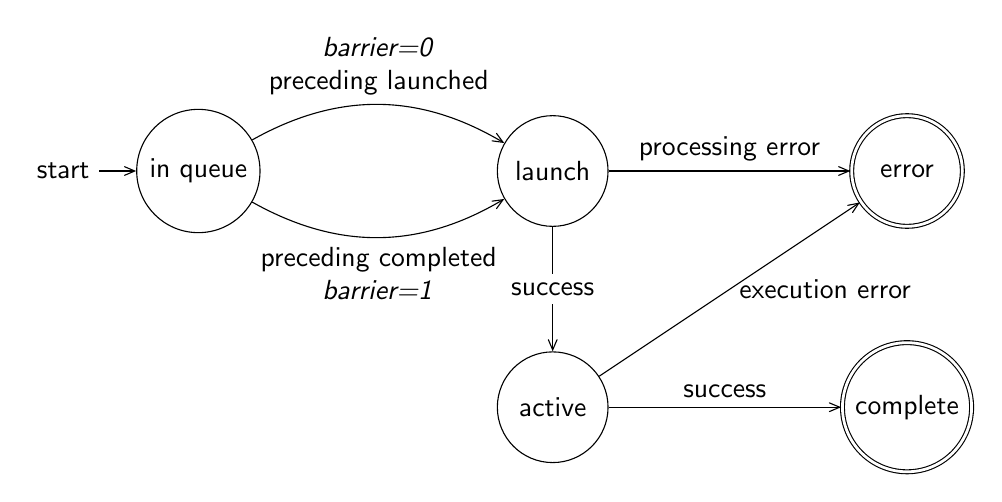
\begin{tikzpicture}
[auto,on grid,node distance=4.5cm,state/.style={circle,draw,minimum size=40pt}]
   \node[state,initial]                 (s0) {in queue};
   \node[state,right=4.5cm of s0]       (s1) {launch};
   \node[state,below=3cm of s1]       (s2) {active};
   \node[state,accepting,double distance=1pt,right=of s1]   (s3) {error};
   \node[state,accepting,double distance=1pt,right=of s2]   (s4) {complete};
   \path[->]
     (s0) edge[bend right]  node[text width=3cm,align=center,below] {preceding completed\\\textit{barrier=1}} (s1)
          edge[bend left] node[text width=3cm,align=center,above]{\textit{barrier=0}\\preceding launched} (s1)
     (s1) edge  node {processing error} (s3)
          edge  node[anchor=center,fill=white,opacity=1] {success} (s2)
     (s2) edge  node{success} (s4)
          edge  node[right]{execution error} (s3)
     ;
\end{tikzpicture}
  \centering
  \caption{Packet State Diagram}
  \label{fig:packetstate}
\end{figure}

\begin{description}[itemsep=2pt,leftmargin=0cm, labelindent=0cm]
\item[In queue] The packet processor has not started to parse the current
  packet.  The transition to the launch state only occurs after all the
  preceding packets have completed their execution if the \reffld{barrier} bit
  is set in the header. If the bit is not set, the transition occurs after the
  preceding packets have finished their launch phase. In other words, while the
  packet processor is required to launch any consecutive two packets in order,
  it is not required to complete them in order unless the barrier bit of the
  second packet is set.

\item[Launch] The packet is being parsed, but it did not start executing. This
  phase finalizes by applying an acquire memory fence with the scope indicated
  by the \reffld{acquire_fence_scope} header field.  Memory fences are discussed
  in~\cite{prm}, Section 6.2.6.

  If an error is detected during launch, the queue transitions to the error
  state and the event callback associated with the queue (if present) is
  invoked. The runtime passes a status code to the callback that indicates the
  source of the problem.  The following status codes might be returned:
  \begin{description}[itemsep=1.5pt,labelindent=.5cm]
  \item[\hsaref{HSA_STATUS_ERROR_INVALID_PACKET_FORMAT}] Malformed AQL
    packet. This could happen if, for example, the packet header type is invalid.
  \item[\hsaref{HSA_STATUS_ERROR_OUT_OF_RESOURCES}] The packet processor is
    unable to allocate the resources required by the launch. This could happen
    if, for example, a Dispatch packet requests more group memory than the size
    of the group memory declared by the corresponding component.
  \end{description}
\item[Active] The execution of the packet has started.

  If an error is detected during this phase, the queue transitions to the error
  state, a release fence is applied to the packet with the scope indicated by
  the \reffld{release_fence_scope} header field, and the completion signal (if
  present) is assigned a negative value. There is no invocation of the callback
  associated with the queue.

  If no error is detected, the transition to the complete state happens when the
  associated task finishes (in the case of Dispatch and Agent Dispatch packets),
  or when the dependencies are satisfied (in the case of a Barrier packet).

\item[Complete] A memory release fence is applied with the scope indicated by
  the \reffld{release_fence_scope} header field, and the completion signal (if
  present) decremented.

\item[Error] An error was encountered during the launch or active phases. No
  further packets will be launched on the queue. The queue cannot be recovered,
  but only inactivated or destroyed. If the application passes the queue as an
  argument to any HSA function other than \hsaref{hsa_queue_inactivate} or
  \hsaref{hsa_queue_destroy}, the behavior is undefined.

\end{description}

\subsection{API}
\makeatletter{}

\subsubsection{hsa_\-packet_\-type_\-t}
\vspace{-5.5mm}\begin{mylongtable}{@{}p{\textwidth}}
\rule{0pt}{3ex}typedef enum \{\\\hspace{1.7em}\hypertarget{group__aql_1gga35a04bfe654a1c980ac904cafd6373a1a4f31bfb4b09cd05fd921b856d711f2a2}{\refenu{HSA_\-PACKET_\-TYPE_\-ALWAYS_\-RESERVED}} = 0,\\
\hspace{1.7em}\hypertarget{group__aql_1gga35a04bfe654a1c980ac904cafd6373a1a9030931b8fe80fb9add8c796cd8886c5}{\refenu{HSA_\-PACKET_\-TYPE_\-INVALID}} = 1,\\
\hspace{1.7em}\hypertarget{group__aql_1gga35a04bfe654a1c980ac904cafd6373a1aeb97ed75df70d88767647a67265e4e59}{\refenu{HSA_\-PACKET_\-TYPE_\-DISPATCH}} = 2,\\
\hspace{1.7em}\hypertarget{group__aql_1gga35a04bfe654a1c980ac904cafd6373a1a33877d0c8ec83f59d3a2f9d3ecbb32da}{\refenu{HSA_\-PACKET_\-TYPE_\-BARRIER}} = 3,\\
\hspace{1.7em}\hypertarget{group__aql_1gga35a04bfe654a1c980ac904cafd6373a1aeb8ddfcceb12c29b12f52609e7bb7ce2}{\refenu{HSA_\-PACKET_\-TYPE_\-AGENT_\-DISPATCH}} = 4\\
\} \hypertarget{group__aql_1ga35a04bfe654a1c980ac904cafd6373a1}{\textbf{hsa_\-packet_\-type_\-t}};\rule[-2ex]{0pt}{0pt}\end{mylongtable}
\vspace{-2mm}Packet type.

\noindent\textbf{Values}\\[-5mm]
\begin{longtable}{@{\hspace{2em}}p{\linewidth-2em}}
\hspace{-2em}\refenu{HSA_\-PACKET_\-TYPE_\-ALWAYS_\-RESERVED}\\Initial type of any packet when the queue is created. A packet processor must not process a packet of this type. All queues support this packet type.\\[2mm]
\hspace{-2em}\refenu{HSA_\-PACKET_\-TYPE_\-INVALID}\\The packet has been processed in the past, but has not been reassigned to the packet processor. A packet processor must not process a packet of this type. All queues support this packet type.\\[2mm]
\hspace{-2em}\refenu{HSA_\-PACKET_\-TYPE_\-DISPATCH}\\Packet used by HSA agents for dispatching jobs to HSA components. Not all queues support packets of this type (see \hyperlink{group__queue_1ga1145b01f6d9e2670179a22c92db39413}{hsa_\-queue_\-feature_\-t}).\\[2mm]
\hspace{-2em}\refenu{HSA_\-PACKET_\-TYPE_\-BARRIER}\\Packet used by HSA agents to delay processing of subsequent packets, and to express complex dependencies between multiple packets. All queues support this packet type.\\[2mm]
\hspace{-2em}\refenu{HSA_\-PACKET_\-TYPE_\-AGENT_\-DISPATCH}\\Packet used by HSA agents for dispatching jobs to HSA agents. Not all queues support packets of this type (see \hyperlink{group__queue_1ga1145b01f6d9e2670179a22c92db39413}{hsa_\-queue_\-feature_\-t}).
\end{longtable}

\subsubsection{hsa_\-fence_\-scope_\-t}
\vspace{-5.5mm}\begin{mylongtable}{@{}p{\textwidth}}
\rule{0pt}{3ex}typedef enum \{\\\hspace{1.7em}\hypertarget{group__aql_1gga6c1a86878de5b0f980202ad7e4e8d42aa5dc7b942cd56f91094a088435027be2c}{\refenu{HSA_\-FENCE_\-SCOPE_\-NONE}} = 0,\\
\hspace{1.7em}\hypertarget{group__aql_1gga6c1a86878de5b0f980202ad7e4e8d42aa9818589db02bc7c0639652eccd64c95d}{\refenu{HSA_\-FENCE_\-SCOPE_\-COMPONENT}} = 1,\\
\hspace{1.7em}\hypertarget{group__aql_1gga6c1a86878de5b0f980202ad7e4e8d42aa6ecb203c10f12ec4bcf475d527c3a870}{\refenu{HSA_\-FENCE_\-SCOPE_\-SYSTEM}} = 2\\
\} \hypertarget{group__aql_1ga6c1a86878de5b0f980202ad7e4e8d42a}{\textbf{hsa_\-fence_\-scope_\-t}};\rule[-2ex]{0pt}{0pt}\end{mylongtable}
\vspace{-2mm}Scope of the memory fence operation associated with a packet.

\noindent\textbf{Values}\\[-5mm]
\begin{longtable}{@{\hspace{2em}}p{\linewidth-2em}}
\hspace{-2em}\refenu{HSA_\-FENCE_\-SCOPE_\-NONE}\\No scope. Can be only used in the \textit{acquire_\-fence_\-scope} field of a Barrier packet.\\[2mm]
\hspace{-2em}\refenu{HSA_\-FENCE_\-SCOPE_\-COMPONENT}\\The fence is applied with component scope for the global segment.\\[2mm]
\hspace{-2em}\refenu{HSA_\-FENCE_\-SCOPE_\-SYSTEM}\\The fence is applied with system scope for the global segment.
\end{longtable}

\subsubsection{hsa_\-packet_\-header_\-t}
\vspace{-5.5mm}\begin{mylongtable}{@{}p{\textwidth}}
\rule{0pt}{3ex}typedef struct  hsa_packet_header_s \{\\
\hspace{1.7em}\hyperlink{group__aql_1ga35a04bfe654a1c980ac904cafd6373a1}{hsa_\-packet_\-type_\-t} \reffld{type} : 8;\\
\hspace{1.7em}uint16_\-t \reffld{barrier} : 1;\\
\hspace{1.7em}\hyperlink{group__aql_1ga6c1a86878de5b0f980202ad7e4e8d42a}{hsa_\-fence_\-scope_\-t} \reffld{acquire_\-fence_\-scope} : 2;\\
\hspace{1.7em}\hyperlink{group__aql_1ga6c1a86878de5b0f980202ad7e4e8d42a}{hsa_\-fence_\-scope_\-t} \reffld{release_\-fence_\-scope} : 2;\\
\hspace{1.7em}uint16_\-t \reffld{reserved} : 3;\\
\}  \hypertarget{group__aql_1gaa3c2c06919444f5f848db2749a85ebb2}{\textbf{hsa_\-packet_\-header_\-t}}\rule[-2ex]{0pt}{0pt}
\end{mylongtable}

\vspace{-2mm}AQL packet header.

\noindent\textbf{Data Fields}\\[-6mm]
\begin{longtable}{@{}>{\hangindent=2em}p{\textwidth}}
\reffld{type}\\\hspace{2em}Packet type.\\[2mm]
\reffld{barrier}\\\hspace{2em}If set, the processing of the current packet only launches when all preceding packets (within the same queue) are complete.\\[2mm]
\reffld{acquire_\-fence_\-scope}\\\hspace{2em}Determines the scope and type of the memory fence operation applied before the packet enters the active phase. Must be \hyperlink{group__aql_1gga6c1a86878de5b0f980202ad7e4e8d42aa5dc7b942cd56f91094a088435027be2c}{HSA_\-FENCE_\-SCOPE_\-NONE} for Barrier packets.\\[2mm]
\reffld{release_\-fence_\-scope}\\\hspace{2em}Determines the scope and type of the memory fence operation applied after kernel completion but before the packet is completed.\\[2mm]
\reffld{reserved}\\\hspace{2em}Must be 0.
\end{longtable}



\subsubsection{hsa_\-dispatch_\-packet_\-t}
\vspace{-5.5mm}\begin{mylongtable}{@{}p{\textwidth}}
\rule{0pt}{3ex}typedef struct  hsa_dispatch_packet_s \{\\
\hspace{1.7em}\hyperlink{group__aql_1gaa3c2c06919444f5f848db2749a85ebb2}{hsa_\-packet_\-header_\-t} \reffld{header};\\
\hspace{1.7em}uint16_\-t \reffld{dimensions} : 2;\\
\hspace{1.7em}uint16_\-t \reffld{reserved} : 14;\\
\hspace{1.7em}uint16_\-t \reffld{workgroup_\-size_\-x};\\
\hspace{1.7em}uint16_\-t \reffld{workgroup_\-size_\-y};\\
\hspace{1.7em}uint16_\-t \reffld{workgroup_\-size_\-z};\\
\hspace{1.7em}uint16_\-t \reffld{reserved2};\\
\hspace{1.7em}uint32_\-t \reffld{grid_\-size_\-x};\\
\hspace{1.7em}uint32_\-t \reffld{grid_\-size_\-y};\\
\hspace{1.7em}uint32_\-t \reffld{grid_\-size_\-z};\\
\hspace{1.7em}uint32_\-t \reffld{private_\-segment_\-size};\\
\hspace{1.7em}uint32_\-t \reffld{group_\-segment_\-size};\\
\hspace{1.7em}uint64_\-t \reffld{kernel_\-object_\-address};\\
\hspace{1.7em}uint64_\-t \reffld{kernarg_\-address};\\
\hspace{1.7em}uint64_\-t \reffld{reserved3};\\
\hspace{1.7em}\hyperlink{group__signals_1gacad8ed7c850275ab33f584967bc0b178}{hsa_\-signal_\-t} \reffld{completion_\-signal};\\
\}  \hypertarget{group__aql_1ga85f6aed8bb5132a5949cdec84147e8a3}{\textbf{hsa_\-dispatch_\-packet_\-t}}\rule[-2ex]{0pt}{0pt}
\end{mylongtable}

\vspace{-2mm}AQL Dispatch packet.

\noindent\textbf{Data Fields}\\[-6mm]
\begin{longtable}{@{}>{\hangindent=2em}p{\textwidth}}
\reffld{header}\\\hspace{2em}Packet header.\\[2mm]
\reffld{dimensions}\\\hspace{2em}Number of dimensions specified in the grid size. Valid values are 1, 2, or 3.\\[2mm]
\reffld{reserved}\\\hspace{2em}Reserved, must be 0.\\[2mm]
\reffld{workgroup_\-size_\-x}\\\hspace{2em}X dimension of work-group, in work-items. Must be greater than 0.\\[2mm]
\reffld{workgroup_\-size_\-y}\\\hspace{2em}Y dimension of work-group, in work-items. Must be greater than 0. If \textit{dimensions} is 1, the only valid value is 1.\\[2mm]
\reffld{workgroup_\-size_\-z}\\\hspace{2em}Z dimension of work-group, in work-items. Must be greater than 0. If \textit{dimensions} is 1 or 2, the only valid value is 1.\\[2mm]
\reffld{reserved2}\\\hspace{2em}Reserved. Must be 0.\\[2mm]
\reffld{grid_\-size_\-x}\\\hspace{2em}X dimension of grid, in work-items. Must be greater than 0. Must not be smaller than \textit{workgroup_\-size_\-x}.\\[2mm]
\reffld{grid_\-size_\-y}\\\hspace{2em}Y dimension of grid, in work-items. Must be greater than 0. If \textit{dimensions} is 1, the only valid value is 1. Must not be smaller than \textit{workgroup_\-size_\-y}.\\[2mm]
\reffld{grid_\-size_\-z}\\\hspace{2em}Z dimension of grid, in work-items. Must be greater than 0. If \textit{dimensions} is 1 or 2, the only valid value is 1. Must not be smaller than \textit{workgroup_\-size_\-z}.\\[2mm]
\reffld{private_\-segment_\-size}\\\hspace{2em}Size in bytes of private memory allocation request (per work-item).\\[2mm]
\reffld{group_\-segment_\-size}\\\hspace{2em}Size in bytes of group memory allocation request (per work-group). Must not be less than the sum of the group memory used by the kernel (and the functions it calls directly or indirectly) and the dynamically allocated group segment variables.\\[2mm]
\reffld{kernel_\-object_\-address}\\\hspace{2em}Address of an object in memory that includes an implementation-defined executable ISA image for the kernel.\\[2mm]
\reffld{kernarg_\-address}\\\hspace{2em}Pointer to a buffer containing the kernel arguments. Might be 0.\\
\hspace{2em}The buffer must be allocated using \hyperlink{group__memory_1ga39f7943b93aa2bb754726fc74d929426}{\reffun{hsa_\-memory_\-allocate}}, and must not be modified once the Dispatch packet is enqueued until the dispatch has completed execution.\\[2mm]
\reffld{reserved3}\\\hspace{2em}Reserved. Must be 0.\\[2mm]
\reffld{completion_\-signal}\\\hspace{2em}Signal used to indicate completion of the job. Might be 0 (no signal).
\end{longtable}



\subsubsection{hsa_\-agent_\-dispatch_\-packet_\-t}
\vspace{-5.5mm}\begin{mylongtable}{@{}p{\textwidth}}
\rule{0pt}{3ex}typedef struct  hsa_agent_dispatch_packet_s \{\\
\hspace{1.7em}\hyperlink{group__aql_1gaa3c2c06919444f5f848db2749a85ebb2}{hsa_\-packet_\-header_\-t} \reffld{header};\\
\hspace{1.7em}uint16_\-t \reffld{type};\\
\hspace{1.7em}uint32_\-t \reffld{reserved2};\\
\hspace{1.7em}uint64_\-t \reffld{return_\-address};\\
\hspace{1.7em}uint64_\-t \reffld{arg}[4];\\
\hspace{1.7em}uint64_\-t \reffld{reserved3};\\
\hspace{1.7em}\hyperlink{group__signals_1gacad8ed7c850275ab33f584967bc0b178}{hsa_\-signal_\-t} \reffld{completion_\-signal};\\
\}  \hypertarget{group__aql_1gaf1fa68d31bcdc7c0eb772e11179520b8}{\textbf{hsa_\-agent_\-dispatch_\-packet_\-t}}\rule[-2ex]{0pt}{0pt}
\end{mylongtable}

\vspace{-2mm}Agent Dispatch packet.

\noindent\textbf{Data Fields}\\[-6mm]
\begin{longtable}{@{}>{\hangindent=2em}p{\textwidth}}
\reffld{header}\\\hspace{2em}Packet header.\\[2mm]
\reffld{type}\\\hspace{2em}The function to be performed by the destination HSA Agent. The type value is split into the following ranges: 0x0000:0x3FFF (vendor specific), 0x4000:0x7FFF (HSA runtime) 0x8000:0xFFFF (application defined).\\[2mm]
\reffld{reserved2}\\\hspace{2em}Reserved. Must be 0.\\[2mm]
\reffld{return_\-address}\\\hspace{2em}Address where to store the function return values, if any.\\[2mm]
\reffld{arg}\\\hspace{2em}Function arguments.\\[2mm]
\reffld{reserved3}\\\hspace{2em}Reserved. Must be 0.\\[2mm]
\reffld{completion_\-signal}\\\hspace{2em}Signal used to indicate completion of the job. Might be 0 (no signal).
\end{longtable}



\subsubsection{hsa_\-barrier_\-packet_\-t}
\vspace{-5.5mm}\begin{mylongtable}{@{}p{\textwidth}}
\rule{0pt}{3ex}typedef struct  hsa_barrier_packet_s \{\\
\hspace{1.7em}\hyperlink{group__aql_1gaa3c2c06919444f5f848db2749a85ebb2}{hsa_\-packet_\-header_\-t} \reffld{header};\\
\hspace{1.7em}uint16_\-t \reffld{reserved2};\\
\hspace{1.7em}uint32_\-t \reffld{reserved3};\\
\hspace{1.7em}\hyperlink{group__signals_1gacad8ed7c850275ab33f584967bc0b178}{hsa_\-signal_\-t} \reffld{dep_\-signal}[5];\\
\hspace{1.7em}uint64_\-t \reffld{reserved4};\\
\hspace{1.7em}\hyperlink{group__signals_1gacad8ed7c850275ab33f584967bc0b178}{hsa_\-signal_\-t} \reffld{completion_\-signal};\\
\}  \hypertarget{group__aql_1ga4982b10808ad313616f2e1be8fca656b}{\textbf{hsa_\-barrier_\-packet_\-t}}\rule[-2ex]{0pt}{0pt}
\end{mylongtable}

\vspace{-2mm}Barrier packet.

\noindent\textbf{Data Fields}\\[-6mm]
\begin{longtable}{@{}>{\hangindent=2em}p{\textwidth}}
\reffld{header}\\\hspace{2em}Packet header.\\[2mm]
\reffld{reserved2}\\\hspace{2em}Reserved. Must be 0.\\[2mm]
\reffld{reserved3}\\\hspace{2em}Reserved. Must be 0.\\[2mm]
\reffld{dep_\-signal}\\\hspace{2em}Array of dependent signal objects. Entries with value 0 are valid and are interpreted by the packet processor as satisfied dependencies.\\[2mm]
\reffld{reserved4}\\\hspace{2em}Reserved. Must be 0.\\[2mm]
\reffld{completion_\-signal}\\\hspace{2em}Signal used to indicate completion of the job. Might be 0 (no signal).
\end{longtable}

 

\section{Memory}\label{sec:memory}

One of the key features of HSA is its ability to share global pointers between
the host application and code executing on any component in a coherent
fashion. An application can directly pass a buffer allocated on the host (for
example, using malloc) to a kernel dispatched in any component. Kernels might
also access memory that is not in the coherent, global segment.

The HSA runtime API provides a compact set of functions for inspecting
the memory \emph{regions} that are accessible from  an agent, and (if applicable)
allocating memory on those regions from the host.

A memory region represents a block of contiguous memory that is directly
accessible by an agent, and exposes properties about the block of memory and how
it is accessed from that particular agent. The same block of memory -virtual or
physical- might be accessible from multiple agents, but the runtime creates a
unique region on every agent to represent the memory block. The characteristics
of a memory region include its size, addressability, access speed, and
corresponding memory segment. One agent might be able to access multiple regions
within the same segment.

The function \hsaref{hsa_agent_iterate_regions} can be used to inspect the set
of regions associated with an agent. Implementations of
\hsaref{hsa_agent_iterate_regions} are required to report the following
regions on every agent:
\begin{itemize}[itemsep=1pt,topsep=3pt,partopsep=0pt]
\item A region that starts at address 0, and is located in the global
  segment. This corresponds to the coherent, primary HSA memory type. All the
  regions with these characteristics should have identical sizes.
\item A region that is located in the global segment and can be used to allocate
  backing storage for the kernarg segment: \hsaref{HSA_REGION_FLAG_KERNARG} is
  true, and \hsaref{HSA_REGION_INFO_ALLOC_MAX_SIZE} is not 0. All the regions
  with these characteristics should have identical sizes.
\end{itemize}

If the application can allocate memory in a region using
\hsaref{hsa_memory_allocate}, the value of the attribute
\hsaref{HSA_REGION_INFO_ALLOC_MAX_SIZE} is different from zero. The runtime
allocator can only be used to allocate memory in the global segment. Memory in
the private, group and kernarg segments is automatically allocated when a
Dispatch packet is launched.

When the application no longer needs a buffer allocated using
\hsaref{hsa_memory_allocate}, it invokes \hsaref{hsa_memory_free} to release the
memory. The application shall not release a runtime-allocated buffer using
standard libraries (for example, free). Conversely, the runtime deallocator
cannot be used to release memory allocated using standard libraries (for
example, malloc).

If a buffer created in the host is also accessed by a component, applications
are encouraged to \emph{register} the corresponding address range beforehand
using the \hsaref{hsa_memory_register} function. While kernels running on HSA
components can access any regular host pointer, a registered buffer might
result on improved access performance.  When the application no longer needs to
access a registered buffer, it should deregister that virtual address range by
invoking \hsaref{hsa_memory_deregister}.

\subsection{Example - passing arguments to a kernel}\label{ex:kernarg_dispatch}
In the kernel setup example listed in Section~\ref{dispatch-packet}, the kernel
receives no arguments:
\begin{lstlisting}
// Indicate which ISA to run. The application is expected to have finalized a kernel (for example, using the finalization API).
// We will assume that the kernel object location is stored in KERNEL_ADDRESS
dispatch_packet->kernel_object_address = (uint64_t) KERNEL_ADDRESS;

// Assume our kernel receives no arguments.
dispatch_packet->kernarg_address = 0;
\end{lstlisting}
Let's assume now that the kernel expects a single argument, a signal handle. The
application needs to populate the \reffld{kernarg_address} field of the Dispatch
packet with the address of a buffer containing the signal.

The application searches for a memory region that can be used to allocate
backing storage for the kernarg segment. Once found, it reserves enough space to
hold the signal argument. While the actual amount of memory to be allocated is
determined by the finalizer, for simplicity we will assume that it matches the
natural size of the signal type, 8 bytes.
\begin{lstlisting}
// Indicate which ISA to run. The application is expected to have finalized a kernel (for example, using the finalization API).
// We will assume that the kernel object location is stored in KERNEL_ADDRESS
dispatch_packet->kernel_object_address = (uint64_t) KERNEL_ADDRESS;

hsa_region_t region;
hsa_agent_iterate_regions(component, get_kernarg, &region);
hsa_memory_allocate(region, 8, (void**) &dispatch_packet->kernarg_address);
\end{lstlisting}

, where the definition of \textit{get_kernarg} is:
\lstinputlisting[firstline=50, lastline=60]{example/kernarg_dispatch.c}

Finally, the application stores a signal handle in the buffer.
\begin{lstlisting}
hsa_signal_t* buffer = (hsa_signal_t*) dispatch_packet->kernarg_address;
assert(buffer != NULL);
hsa_signal_t signal;
hsa_signal_create(1, 1, &component, &signal);
*buffer = signal;
\end{lstlisting}
The rest of the dispatch process remains the same.

\subsection{API}
\makeatletter{}

\subsubsection{hsa_\-region_\-t}
\vspace{-5.5mm}\begin{mylongtable}{@{}p{\textwidth}}
\rule{0pt}{3ex}\rule[-2.5ex]{0pt}{0pt}typedef uint64_\-t  \hypertarget{group__memory_1gaa5f6311c53cbe299caebef621e060588}{\textbf{hsa_\-region_\-t}};
\end{mylongtable}\vspace{-3mm}
\vspace{-2mm}A memory region represents a block of contiguous memory that is directly accessible by an agent, and exposes properties about the block of memory and how it is accessed from that particular agent.
\\

\subsubsection{hsa_\-segment_\-t}
\vspace{-5.5mm}\begin{mylongtable}{@{}p{\textwidth}}
\rule{0pt}{3ex}typedef enum \{\\\hspace{1.7em}\hypertarget{group__memory_1gga9aa2ffad72549139936d37692a4214dda0488a507ac10e730a5da4c7e88c9708b}{\refenu{HSA_\-SEGMENT_\-GLOBAL}},\\
\hspace{1.7em}\hypertarget{group__memory_1gga9aa2ffad72549139936d37692a4214dda8973c2316a8b2247b8a2a2f2546cde38}{\refenu{HSA_\-SEGMENT_\-PRIVATE}},\\
\hspace{1.7em}\hypertarget{group__memory_1gga9aa2ffad72549139936d37692a4214ddad3e8c2fe02eb7e9febdacb51dff74d5e}{\refenu{HSA_\-SEGMENT_\-GROUP}},\\
\hspace{1.7em}\hypertarget{group__memory_1gga9aa2ffad72549139936d37692a4214dda79388d7547c31b8b90ada3f6e5470603}{\refenu{HSA_\-SEGMENT_\-KERNARG}},\\
\hspace{1.7em}\hypertarget{group__memory_1gga9aa2ffad72549139936d37692a4214dda9a30a39c5916dd3e21f896442a71357e}{\refenu{HSA_\-SEGMENT_\-READONLY}},\\
\hspace{1.7em}\hypertarget{group__memory_1gga9aa2ffad72549139936d37692a4214dda49c452f1685d135040e411f7f158bacf}{\refenu{HSA_\-SEGMENT_\-SPILL}},\\
\hspace{1.7em}\hypertarget{group__memory_1gga9aa2ffad72549139936d37692a4214ddacf2a4adb39685f23541290167b4b4c60}{\refenu{HSA_\-SEGMENT_\-ARG}}\\
\} \hypertarget{group__memory_1ga9aa2ffad72549139936d37692a4214dd}{\textbf{hsa_\-segment_\-t}};\rule[-2ex]{0pt}{0pt}\end{mylongtable}
\vspace{-2mm}Types of memory segments.

\noindent\textbf{Values}\\[-5mm]
\begin{longtable}{@{\hspace{2em}}p{\linewidth-2em}}
\hspace{-2em}\refenu{HSA_\-SEGMENT_\-GLOBAL}\\Global segment. Used to hold data that is shared by all agents.\\[2mm]
\hspace{-2em}\refenu{HSA_\-SEGMENT_\-PRIVATE}\\Private segment. Used to hold data that is local to a single work-item.\\[2mm]
\hspace{-2em}\refenu{HSA_\-SEGMENT_\-GROUP}\\Group segment. Used to hold data that is shared by the work-items of a work-group.\\[2mm]
\hspace{-2em}\refenu{HSA_\-SEGMENT_\-KERNARG}\\Kernarg segment. Used to pass arguments into a kernel. Memory in this segment is visible to all work-items of the kernel dispatch with which it is associated.\\[2mm]
\hspace{-2em}\refenu{HSA_\-SEGMENT_\-READONLY}\\Read-only segment. Used used to hold data that remains constant during the execution of a kernel dispatch.\\[2mm]
\hspace{-2em}\refenu{HSA_\-SEGMENT_\-SPILL}\\Spill segment. Used to load or store register spills.\\[2mm]
\hspace{-2em}\refenu{HSA_\-SEGMENT_\-ARG}\\Arg segment. Used to pass arguments into and out of functions.
\end{longtable}

\subsubsection{hsa_\-region_\-flag_\-t}
\vspace{-5.5mm}\begin{mylongtable}{@{}p{\textwidth}}
\rule{0pt}{3ex}typedef enum \{\\\hspace{1.7em}\hypertarget{group__memory_1ggafaf486b604f88ca026eecdb8ecce528fa838754411c1344031d8d72e9455a6d4f}{\refenu{HSA_\-REGION_\-FLAG_\-KERNARG}} = 1,\\
\hspace{1.7em}\hypertarget{group__memory_1ggafaf486b604f88ca026eecdb8ecce528fad61659f8c912b5bc2f3122f33980e5bc}{\refenu{HSA_\-REGION_\-FLAG_\-CACHED_\-L1}} = 2,\\
\hspace{1.7em}\hypertarget{group__memory_1ggafaf486b604f88ca026eecdb8ecce528faf73add97df9c1d5a633c1d2a425fd865}{\refenu{HSA_\-REGION_\-FLAG_\-CACHED_\-L2}} = 4,\\
\hspace{1.7em}\hypertarget{group__memory_1ggafaf486b604f88ca026eecdb8ecce528fa859e9d36cfb559b2bafadf523ee6f501}{\refenu{HSA_\-REGION_\-FLAG_\-CACHED_\-L3}} = 8,\\
\hspace{1.7em}\hypertarget{group__memory_1ggafaf486b604f88ca026eecdb8ecce528faea087e334f082aac0b69a7e3f106c66f}{\refenu{HSA_\-REGION_\-FLAG_\-CACHED_\-L4}} = 16\\
\} \hypertarget{group__memory_1gafaf486b604f88ca026eecdb8ecce528f}{\textbf{hsa_\-region_\-flag_\-t}};\rule[-2ex]{0pt}{0pt}\end{mylongtable}
\vspace{-2mm}Region flags.

\noindent\textbf{Values}\\[-5mm]
\begin{longtable}{@{\hspace{2em}}p{\linewidth-2em}}
\hspace{-2em}\refenu{HSA_\-REGION_\-FLAG_\-KERNARG}\\The application can use memory in the region to store kernel arguments, and provide the values for the kernarg segment of a kernel dispatch. If the region is not in the global segment, this flag must not be set.\\[2mm]
\hspace{-2em}\refenu{HSA_\-REGION_\-FLAG_\-CACHED_\-L1}\\Accesses to data in the region are cached in the L1 data cache of the region's agent. If the agent does not have an L1 cache (as reported by the attribute \hyperlink{group__agentinfo_1gga39d0684207d95717d96319573b3e4a42ae7fe21528c215249472e5836631759f4}{HSA_\-AGENT_\-INFO_\-CACHE_\-SIZE}), this flag must not be set.\\[2mm]
\hspace{-2em}\refenu{HSA_\-REGION_\-FLAG_\-CACHED_\-L2}\\Accesses to data in the region are cached in the L2 data cache of the region's agent. If the agent does not have an L2 cache (as reported by the attribute \hyperlink{group__agentinfo_1gga39d0684207d95717d96319573b3e4a42ae7fe21528c215249472e5836631759f4}{HSA_\-AGENT_\-INFO_\-CACHE_\-SIZE}), this flag must not be set.\\[2mm]
\hspace{-2em}\refenu{HSA_\-REGION_\-FLAG_\-CACHED_\-L3}\\Accesses to data in the region are cached in the L3 data cache of the region's agent. If the agent does not have an L3 cache (as reported by the attribute \hyperlink{group__agentinfo_1gga39d0684207d95717d96319573b3e4a42ae7fe21528c215249472e5836631759f4}{HSA_\-AGENT_\-INFO_\-CACHE_\-SIZE}), this flag must not be set.\\[2mm]
\hspace{-2em}\refenu{HSA_\-REGION_\-FLAG_\-CACHED_\-L4}\\Accesses to data in the region are cached in the L4 data cache of the region's agent. If the agent does not have an L4 cache (as reported by the attribute \hyperlink{group__agentinfo_1gga39d0684207d95717d96319573b3e4a42ae7fe21528c215249472e5836631759f4}{HSA_\-AGENT_\-INFO_\-CACHE_\-SIZE}), this flag must not be set.
\end{longtable}

\subsubsection{hsa_\-region_\-info_\-t}
\vspace{-5.5mm}\begin{mylongtable}{@{}p{\textwidth}}
\rule{0pt}{3ex}typedef enum \{\\\hspace{1.7em}\hypertarget{group__memory_1ggad35755078ff15f645c6c25e7f7ef2707af5033c8ce5609f9055ae0624e04d1c83}{\refenu{HSA_\-REGION_\-INFO_\-BASE}},\\
\hspace{1.7em}\hypertarget{group__memory_1ggad35755078ff15f645c6c25e7f7ef2707a09403f5c83497726504523694b3e86b6}{\refenu{HSA_\-REGION_\-INFO_\-SIZE}},\\
\hspace{1.7em}\hypertarget{group__memory_1ggad35755078ff15f645c6c25e7f7ef2707a92bbdc9ec69d5ed54ea37b4b5c3be58e}{\refenu{HSA_\-REGION_\-INFO_\-AGENT}},\\
\hspace{1.7em}\hypertarget{group__memory_1ggad35755078ff15f645c6c25e7f7ef2707a97869505d019b0800355cab4a21c3403}{\refenu{HSA_\-REGION_\-INFO_\-FLAGS}},\\
\hspace{1.7em}\hypertarget{group__memory_1ggad35755078ff15f645c6c25e7f7ef2707ab2701b5deebcf46596e8f070f6ef27b6}{\refenu{HSA_\-REGION_\-INFO_\-SEGMENT}},\\
\hspace{1.7em}\hypertarget{group__memory_1ggad35755078ff15f645c6c25e7f7ef2707ab846101a22f46f61e0caf1d73cedd414}{\refenu{HSA_\-REGION_\-INFO_\-ALLOC_\-MAX_\-SIZE}},\\
\hspace{1.7em}\hypertarget{group__memory_1ggad35755078ff15f645c6c25e7f7ef2707ab602c01f90962314de88fb887b6f13b3}{\refenu{HSA_\-REGION_\-INFO_\-ALLOC_\-GRANULE}},\\
\hspace{1.7em}\hypertarget{group__memory_1ggad35755078ff15f645c6c25e7f7ef2707af3103bc1328080b236a7847f1bf4998e}{\refenu{HSA_\-REGION_\-INFO_\-ALLOC_\-ALIGNMENT}},\\
\hspace{1.7em}\hypertarget{group__memory_1ggad35755078ff15f645c6c25e7f7ef2707a77389057885a6a331863536fe4c66a5c}{\refenu{HSA_\-REGION_\-INFO_\-BANDWIDTH}},\\
\hspace{1.7em}\hypertarget{group__memory_1ggad35755078ff15f645c6c25e7f7ef2707ab7bb10ceec7634e32c7ad29e6b4a31a0}{\refenu{HSA_\-REGION_\-INFO_\-NODE}}\\
\} \hypertarget{group__memory_1gad35755078ff15f645c6c25e7f7ef2707}{\textbf{hsa_\-region_\-info_\-t}};\rule[-2ex]{0pt}{0pt}\end{mylongtable}
\vspace{-2mm}Attributes of a memory region.

\noindent\textbf{Values}\\[-5mm]
\begin{longtable}{@{\hspace{2em}}p{\linewidth-2em}}
\hspace{-2em}\refenu{HSA_\-REGION_\-INFO_\-BASE}\\Base (starting) address. The type of this attribute is void*.\\[2mm]
\hspace{-2em}\refenu{HSA_\-REGION_\-INFO_\-SIZE}\\Size, in bytes. The type of this attribute is size_\-t.\\[2mm]
\hspace{-2em}\refenu{HSA_\-REGION_\-INFO_\-AGENT}\\Agent associated with this region. The type of this attribute is hsa_\-agent_\-t.\\[2mm]
\hspace{-2em}\refenu{HSA_\-REGION_\-INFO_\-FLAGS}\\Flag mask. The type of this attribute is uint32_\-t, a bit-field of \hyperlink{group__memory_1gafaf486b604f88ca026eecdb8ecce528f}{hsa_\-region_\-flag_\-t} values.\\[2mm]
\hspace{-2em}\refenu{HSA_\-REGION_\-INFO_\-SEGMENT}\\Segment where memory in the region can be used. The type of this attribute is \hyperlink{group__memory_1ga9aa2ffad72549139936d37692a4214dd}{hsa_\-segment_\-t}.\\[2mm]
\hspace{-2em}\refenu{HSA_\-REGION_\-INFO_\-ALLOC_\-MAX_\-SIZE}\\Maximum allocation size in this region, in bytes. A value of 0 indicates that the host cannot allocate memory in the region using \hyperlink{group__memory_1ga39f7943b93aa2bb754726fc74d929426}{\reffun{hsa_\-memory_\-allocate}}. If the value of \hyperlink{group__memory_1ggad35755078ff15f645c6c25e7f7ef2707ab2701b5deebcf46596e8f070f6ef27b6}{HSA_\-REGION_\-INFO_\-SEGMENT} is other than \hyperlink{group__memory_1gga9aa2ffad72549139936d37692a4214dda0488a507ac10e730a5da4c7e88c9708b}{HSA_\-SEGMENT_\-GLOBAL}, the maximum allocation size must be 0. The type of this attribute is size_\-t.\\[2mm]
\hspace{-2em}\refenu{HSA_\-REGION_\-INFO_\-ALLOC_\-GRANULE}\\Allocation granularity of buffers allocated by \hyperlink{group__memory_1ga39f7943b93aa2bb754726fc74d929426}{\reffun{hsa_\-memory_\-allocate}} in this region. The size of a buffer allocated in this region is a multiple of the value of this attribute. If \hyperlink{group__memory_1ggad35755078ff15f645c6c25e7f7ef2707ab846101a22f46f61e0caf1d73cedd414}{HSA_\-REGION_\-INFO_\-ALLOC_\-MAX_\-SIZE} is 0, the allocation granularity must be 0. The type of this attribute is size_\-t.\\[2mm]
\hspace{-2em}\refenu{HSA_\-REGION_\-INFO_\-ALLOC_\-ALIGNMENT}\\Alignment of buffers allocated by \hyperlink{group__memory_1ga39f7943b93aa2bb754726fc74d929426}{\reffun{hsa_\-memory_\-allocate}} in this region. If \hyperlink{group__memory_1ggad35755078ff15f645c6c25e7f7ef2707ab846101a22f46f61e0caf1d73cedd414}{HSA_\-REGION_\-INFO_\-ALLOC_\-MAX_\-SIZE} is 0, the alignment must be 0. Otherwise, it must be a power of 2. The type of this attribute is size_\-t.\\[2mm]
\hspace{-2em}\refenu{HSA_\-REGION_\-INFO_\-BANDWIDTH}\\Peak bandwidth, in MB/s. The type of this attribute is uint32_\-t.\\[2mm]
\hspace{-2em}\refenu{HSA_\-REGION_\-INFO_\-NODE}\\NUMA node associated with this region. The type of this attribute is uint32_\-t.
\end{longtable}

\index[api]{hsa_region_get_info}\subsubsection{hsa_\-region_\-get_\-info}
\vspace{-5.5mm}\begin{mylongtable}{@{}p{\textwidth}}

\pbox{\textwidth}{\hspace{1mm}\\[1mm]\hyperlink{group__status_1gad755322e7ff95456520e8abdbe90d225}{hsa_\-status_\-t} \hypertarget{group__memory_1gaad0ab0056cfee2e5a99270490b942a28}{\textbf{hsa_\-region_\-get_\-info}}(\\\hspace*{1.7em}\hyperlink{group__memory_1gaa5f6311c53cbe299caebef621e060588}{hsa_\-region_\-t} \hsaarg{region},\\\hspace*{1.7em}\hyperlink{group__memory_1gad35755078ff15f645c6c25e7f7ef2707}{hsa_\-region_\-info_\-t} \hsaarg{attribute},\\\hspace*{1.7em}void * \hsaarg{value});\\}\end{mylongtable}
\vspace{-2mm}Get the current value of an attribute of a region.

\noindent\textbf{Parameters}\\[-6mm]
\noindent\begin{longtable}{@{}>{\hangindent=2em}p{\textwidth}}
\hsaarg{region}\\\hspace{2em}(in) A valid region.\\[2mm]
\hsaarg{attribute}\\\hspace{2em}(in) Attribute to query.\\[2mm]
\hsaarg{value}\\\hspace{2em}(out) Pointer to a application-allocated buffer where to store the value of the attribute. If the buffer passed by the application is not large enough to hold the value of \textit{attribute}, the behavior is undefined.
\end{longtable}
\vspace{-5mm}\noindent\textbf{Return Values}\\[-6mm]
\noindent\begin{longtable}{@{}>{\hangindent=2em}p{\linewidth}}
\hyperlink{group__status_1ggad755322e7ff95456520e8abdbe90d225ae382ea0c9c05cce5a60d0317375159cc}{HSA_\-STATUS_\-SUCCESS}\\\hspace{2em}The function has been executed successfully.\\[2mm]
\hyperlink{group__status_1ggad755322e7ff95456520e8abdbe90d225a34ea59ade5bfce95eee935238a99f5b5}{HSA_\-STATUS_\-ERROR_\-NOT_\-INITIALIZED}\\\hspace{2em}The runtime has not been initialized.\\[2mm]
\hyperlink{group__status_1ggad755322e7ff95456520e8abdbe90d225ad63594ac02edec7ae7aa7722c11afcd9}{HSA_\-STATUS_\-ERROR_\-INVALID_\-REGION}\\\hspace{2em}If the region is invalid.\\[2mm]
\hyperlink{group__status_1ggad755322e7ff95456520e8abdbe90d225ac7d3651f75107d2a6a8ba3b25683c030}{HSA_\-STATUS_\-ERROR_\-INVALID_\-ARGUMENT}\\\hspace{2em}If \textit{attribute} is not a valid region attribute, or \textit{value} is NULL.
\end{longtable}
\vspace{-5mm} 


\index[api]{hsa_agent_iterate_regions}\subsubsection{hsa_\-agent_\-iterate_\-regions}
\vspace{-5.5mm}\begin{mylongtable}{@{}p{\textwidth}}

\pbox{\textwidth}{\hspace{1mm}\\[1mm]\hyperlink{group__status_1gad755322e7ff95456520e8abdbe90d225}{hsa_\-status_\-t} \hypertarget{group__memory_1gad595a460e2867a134ec90de63589c0eb}{\textbf{hsa_\-agent_\-iterate_\-regions}}(\\\hspace*{1.7em}\hyperlink{group__agentinfo_1ga27393931438432bb42772bc10f5d4941}{hsa_\-agent_\-t} \hsaarg{agent},\\\hspace*{1.7em}\hyperlink{group__status_1gad755322e7ff95456520e8abdbe90d225}{hsa_\-status_\-t} (*\hsaarg{callback})(\hyperlink{group__memory_1gaa5f6311c53cbe299caebef621e060588}{hsa_\-region_\-t} region, void *data),\\\hspace*{1.7em}void * \hsaarg{data});\\}\end{mylongtable}
\vspace{-2mm}Iterate over the memory regions associated with a given agent, and invoke an application-defined callback on every iteration.

\noindent\textbf{Parameters}\\[-6mm]
\noindent\begin{longtable}{@{}>{\hangindent=2em}p{\textwidth}}
\hsaarg{agent}\\\hspace{2em}(in) A valid agent.\\[2mm]
\hsaarg{callback}\\\hspace{2em}(in) Callback to be invoked once per region that is directly accessible from the agent. The runtime passes two arguments to the callback, the region and the application data. If \textit{callback} returns a status other than \hyperlink{group__status_1ggad755322e7ff95456520e8abdbe90d225ae382ea0c9c05cce5a60d0317375159cc}{HSA_\-STATUS_\-SUCCESS} for a particular iteration, the traversal stops and \hyperlink{group__memory_1gad595a460e2867a134ec90de63589c0eb}{\reffun{hsa_\-agent_\-iterate_\-regions}} returns that status value.\\[2mm]
\hsaarg{data}\\\hspace{2em}(in) Application data that is passed to \textit{callback} on every iteration. Might be NULL.
\end{longtable}
\vspace{-5mm}\noindent\textbf{Return Values}\\[-6mm]
\noindent\begin{longtable}{@{}>{\hangindent=2em}p{\linewidth}}
\hyperlink{group__status_1ggad755322e7ff95456520e8abdbe90d225ae382ea0c9c05cce5a60d0317375159cc}{HSA_\-STATUS_\-SUCCESS}\\\hspace{2em}The function has been executed successfully.\\[2mm]
\hyperlink{group__status_1ggad755322e7ff95456520e8abdbe90d225a34ea59ade5bfce95eee935238a99f5b5}{HSA_\-STATUS_\-ERROR_\-NOT_\-INITIALIZED}\\\hspace{2em}The runtime has not been initialized.\\[2mm]
\hyperlink{group__status_1ggad755322e7ff95456520e8abdbe90d225a3a5d835c109c2d0ad5b9c2771e133e5d}{HSA_\-STATUS_\-ERROR_\-INVALID_\-AGENT}\\\hspace{2em}If the agent is invalid.\\[2mm]
\hyperlink{group__status_1ggad755322e7ff95456520e8abdbe90d225ac7d3651f75107d2a6a8ba3b25683c030}{HSA_\-STATUS_\-ERROR_\-INVALID_\-ARGUMENT}\\\hspace{2em}If \textit{callback} is NULL.
\end{longtable}
\vspace{-5mm} 


\index[api]{hsa_memory_allocate}\subsubsection{hsa_\-memory_\-allocate}
\vspace{-5.5mm}\begin{mylongtable}{@{}p{\textwidth}}

\pbox{\textwidth}{\hspace{1mm}\\[1mm]\hyperlink{group__status_1gad755322e7ff95456520e8abdbe90d225}{hsa_\-status_\-t} \hypertarget{group__memory_1ga39f7943b93aa2bb754726fc74d929426}{\textbf{hsa_\-memory_\-allocate}}(\\\hspace*{1.7em}\hyperlink{group__memory_1gaa5f6311c53cbe299caebef621e060588}{hsa_\-region_\-t} \hsaarg{region},\\\hspace*{1.7em}size_\-t \hsaarg{size},\\\hspace*{1.7em}void ** \hsaarg{ptr});\\}\end{mylongtable}
\vspace{-2mm}Allocate a block of memory in a given region.

\noindent\textbf{Parameters}\\[-6mm]
\noindent\begin{longtable}{@{}>{\hangindent=2em}p{\textwidth}}
\hsaarg{region}\\\hspace{2em}(in) Region where to allocate memory from.\\[2mm]
\hsaarg{size}\\\hspace{2em}(in) Allocation size, in bytes. This value is rounded up to the the nearest multiple of \hyperlink{group__memory_1ggad35755078ff15f645c6c25e7f7ef2707ab602c01f90962314de88fb887b6f13b3}{HSA_\-REGION_\-INFO_\-ALLOC_\-GRANULE} in \textit{region}. Allocations of size 0 are allowed and return a NULL pointer.\\[2mm]
\hsaarg{ptr}\\\hspace{2em}(out) Pointer to the location where to store the base address of the allocated block. The returned base address is aligned to the value of \hyperlink{group__memory_1ggad35755078ff15f645c6c25e7f7ef2707af3103bc1328080b236a7847f1bf4998e}{HSA_\-REGION_\-INFO_\-ALLOC_\-ALIGNMENT} in \textit{region}.
\end{longtable}
\vspace{-5mm}\noindent\textbf{Return Values}\\[-6mm]
\noindent\begin{longtable}{@{}>{\hangindent=2em}p{\linewidth}}
\hyperlink{group__status_1ggad755322e7ff95456520e8abdbe90d225ae382ea0c9c05cce5a60d0317375159cc}{HSA_\-STATUS_\-SUCCESS}\\\hspace{2em}The function has been executed successfully.\\[2mm]
\hyperlink{group__status_1ggad755322e7ff95456520e8abdbe90d225a34ea59ade5bfce95eee935238a99f5b5}{HSA_\-STATUS_\-ERROR_\-NOT_\-INITIALIZED}\\\hspace{2em}The runtime has not been initialized.\\[2mm]
\hyperlink{group__status_1ggad755322e7ff95456520e8abdbe90d225a1a77fcf36d0d140874c4361ab093eff7}{HSA_\-STATUS_\-ERROR_\-OUT_\-OF_\-RESOURCES}\\\hspace{2em}If no memory is available.\\[2mm]
\hyperlink{group__status_1ggad755322e7ff95456520e8abdbe90d225ad63594ac02edec7ae7aa7722c11afcd9}{HSA_\-STATUS_\-ERROR_\-INVALID_\-REGION}\\\hspace{2em}If the region is invalid.\\[2mm]
\hyperlink{group__status_1ggad755322e7ff95456520e8abdbe90d225ac818189ff640d38ce13558e72daddb75}{HSA_\-STATUS_\-ERROR_\-INVALID_\-ALLOCATION}\\\hspace{2em}If the host is not allowed to allocate memory in \textit{region}, or \textit{size} is greater than the value of HSA_REGION_INFO_ALLOC_MAX_SIZE in \textit{region}.\\[2mm]
\hyperlink{group__status_1ggad755322e7ff95456520e8abdbe90d225ac7d3651f75107d2a6a8ba3b25683c030}{HSA_\-STATUS_\-ERROR_\-INVALID_\-ARGUMENT}\\\hspace{2em}If \textit{ptr} is NULL.
\end{longtable}
\vspace{-5mm} 


\index[api]{hsa_memory_free}\subsubsection{hsa_\-memory_\-free}
\vspace{-5.5mm}\begin{mylongtable}{@{}p{\textwidth}}

\pbox{\textwidth}{\hspace{1mm}\\[1mm]\hyperlink{group__status_1gad755322e7ff95456520e8abdbe90d225}{hsa_\-status_\-t} \hypertarget{group__memory_1gaf968e8053981351ec0b16a04aeb51a8e}{\textbf{hsa_\-memory_\-free}}(\\\hspace*{1.7em}void * \hsaarg{ptr});\\}\end{mylongtable}
\vspace{-2mm}Deallocate a block of memory previously allocated using \hyperlink{group__memory_1ga39f7943b93aa2bb754726fc74d929426}{\reffun{hsa_\-memory_\-allocate}}.

\noindent\textbf{Parameters}\\[-6mm]
\noindent\begin{longtable}{@{}>{\hangindent=2em}p{\textwidth}}
\hsaarg{ptr}\\\hspace{2em}(in) Pointer to a memory block. If \textit{ptr} is NULL, no action is performed.
\end{longtable}
\vspace{-5mm}\noindent\textbf{Return Values}\\[-6mm]
\noindent\begin{longtable}{@{}>{\hangindent=2em}p{\linewidth}}
\hyperlink{group__status_1ggad755322e7ff95456520e8abdbe90d225ae382ea0c9c05cce5a60d0317375159cc}{HSA_\-STATUS_\-SUCCESS}\\\hspace{2em}The function has been executed successfully.\\[2mm]
\hyperlink{group__status_1ggad755322e7ff95456520e8abdbe90d225a34ea59ade5bfce95eee935238a99f5b5}{HSA_\-STATUS_\-ERROR_\-NOT_\-INITIALIZED}\\\hspace{2em}The runtime has not been initialized.
\end{longtable}
\vspace{-5mm} 


\index[api]{hsa_memory_register}\subsubsection{hsa_\-memory_\-register}
\vspace{-5.5mm}\begin{mylongtable}{@{}p{\textwidth}}

\pbox{\textwidth}{\hspace{1mm}\\[1mm]\hyperlink{group__status_1gad755322e7ff95456520e8abdbe90d225}{hsa_\-status_\-t} \hypertarget{group__memory_1gaa4d4efc5ba903ea29587392aa1c8a267}{\textbf{hsa_\-memory_\-register}}(\\\hspace*{1.7em}void * \hsaarg{address},\\\hspace*{1.7em}size_\-t \hsaarg{size});\\}\end{mylongtable}
\vspace{-2mm}Register memory.

\noindent\textbf{Parameters}\\[-6mm]
\noindent\begin{longtable}{@{}>{\hangindent=2em}p{\textwidth}}
\hsaarg{address}\\\hspace{2em}(in) A pointer to the base of the memory region to be registered. If a NULL pointer is passed, no operation is performed.\\[2mm]
\hsaarg{size}\\\hspace{2em}(in) Requested registration size in bytes. A size of zero is only allowed if \textit{address} is NULL.
\end{longtable}
\vspace{-5mm}\noindent\textbf{Return Values}\\[-6mm]
\noindent\begin{longtable}{@{}>{\hangindent=2em}p{\linewidth}}
\hyperlink{group__status_1ggad755322e7ff95456520e8abdbe90d225ae382ea0c9c05cce5a60d0317375159cc}{HSA_\-STATUS_\-SUCCESS}\\\hspace{2em}The function has been executed successfully.\\[2mm]
\hyperlink{group__status_1ggad755322e7ff95456520e8abdbe90d225a34ea59ade5bfce95eee935238a99f5b5}{HSA_\-STATUS_\-ERROR_\-NOT_\-INITIALIZED}\\\hspace{2em}The runtime has not been initialized.\\[2mm]
\hyperlink{group__status_1ggad755322e7ff95456520e8abdbe90d225a1a77fcf36d0d140874c4361ab093eff7}{HSA_\-STATUS_\-ERROR_\-OUT_\-OF_\-RESOURCES}\\\hspace{2em}If there is a failure in allocating the necessary resources.\\[2mm]
\hyperlink{group__status_1ggad755322e7ff95456520e8abdbe90d225ac7d3651f75107d2a6a8ba3b25683c030}{HSA_\-STATUS_\-ERROR_\-INVALID_\-ARGUMENT}\\\hspace{2em}If \textit{size} is 0 but \textit{address} is not NULL.
\end{longtable}
\vspace{-5mm}\noindent\textbf{Description}\\[1mm]
Registering a buffer serves as an indication to the runtime that the passed buffer might be accessed from a component other than the host. Registration is a performance hint that allows the runtime implementation to know which buffers will be accessed by some of the components ahead of time.\\[2mm]
Registrations should not overlap. 


\index[api]{hsa_memory_deregister}\subsubsection{hsa_\-memory_\-deregister}
\vspace{-5.5mm}\begin{mylongtable}{@{}p{\textwidth}}

\pbox{\textwidth}{\hspace{1mm}\\[1mm]\hyperlink{group__status_1gad755322e7ff95456520e8abdbe90d225}{hsa_\-status_\-t} \hypertarget{group__memory_1gada8edf9499aedc160bc3432fe6b170f3}{\textbf{hsa_\-memory_\-deregister}}(\\\hspace*{1.7em}void * \hsaarg{address},\\\hspace*{1.7em}size_\-t \hsaarg{size});\\}\end{mylongtable}
\vspace{-2mm}Deregister memory previously registered using \hyperlink{group__memory_1gaa4d4efc5ba903ea29587392aa1c8a267}{\reffun{hsa_\-memory_\-register}}.

\noindent\textbf{Parameters}\\[-6mm]
\noindent\begin{longtable}{@{}>{\hangindent=2em}p{\textwidth}}
\hsaarg{address}\\\hspace{2em}(in) A pointer to the base of the memory region to be deregistered. If a NULL pointer is passed, no operation is performed.\\[2mm]
\hsaarg{size}\\\hspace{2em}(in) Size of the region to be deregistered.
\end{longtable}
\vspace{-5mm}\noindent\textbf{Return Values}\\[-6mm]
\noindent\begin{longtable}{@{}>{\hangindent=2em}p{\linewidth}}
\hyperlink{group__status_1ggad755322e7ff95456520e8abdbe90d225ae382ea0c9c05cce5a60d0317375159cc}{HSA_\-STATUS_\-SUCCESS}\\\hspace{2em}The function has been executed successfully.\\[2mm]
\hyperlink{group__status_1ggad755322e7ff95456520e8abdbe90d225a34ea59ade5bfce95eee935238a99f5b5}{HSA_\-STATUS_\-ERROR_\-NOT_\-INITIALIZED}\\\hspace{2em}The runtime has not been initialized.
\end{longtable}
\vspace{-5mm}\noindent\textbf{Description}\\[1mm]
If the memory interval being deregistered does not match a previous registration (start and end addresses), the behavior is undefined. 
 




\section{Extensions to the Core Runtime API}\label{extensions}

Extensions to the Core API can be optional (multi-vendor) or vendor
specific. The difference is in the naming scheme used for the symbols (defines,
structures, functions, etc.) associated with the function:

\begin{itemize}
\item Symbols for multi-vendor extensions defined in the global namespace must
  use the \emph{hsa_ext_} prefix in their identifiers.
\item Symbols for single vendor extensions defined in the global namespace must
  use the \emph{hsa_svext_VENDOR_} prefix in their identifiers. Company names
  must be registered with the HSA Foundation, must be unique, and may be
  abbreviated to improve the readability of the symbols.
\end{itemize}

Any constant definitions in the extension (\#define or enumeration values) use
the same naming convention, except using all capital letters.

The symbols for all vendor extensions (both single-vendor and multi-vendor) are
captured in the file {\bf hsa/vendor_extensions.h}. This file is maintained by
the HSA Foundation. This file includes the enumeration \hsaref{hsa_extension_t}
which defines a unique code for each vendor extension and multi-vendor
extension. Vendors can reserve enumeration encodings through the HSA
Foundation. Multi-vendor enumerations begin at the value of
\hsaref{HSA_EXT_START}, while single-vendor enumerations begin at
\hsaref{HSA_SVEXT_START}

\subsection{API}
\makeatletter{}

\subsubsection{hsa_\-extension_\-t}
\vspace{-5.5mm}\begin{mylongtable}{@{}p{\textwidth}}
\rule{0pt}{3ex}typedef enum \{\\\hspace{1.7em}\hypertarget{group__extensions_1gga6a8dade2a7681dbd98a88029b1dbb5f3aac4cd309e9f72222b33b9c39cedf59b6}{\refenu{HSA_\-EXT_\-START}} = 0,\\
\hspace{1.7em}\hypertarget{group__extensions_1gga6a8dade2a7681dbd98a88029b1dbb5f3a2ca4542cee2ee2bcbc488b55267fd95b}{\refenu{HSA_\-EXT_\-FINALIZER}} = HSA_\-EXT_\-START,\\
\hspace{1.7em}\hypertarget{group__extensions_1gga6a8dade2a7681dbd98a88029b1dbb5f3a86fef6b16a18f71f235f9b8f7902b720}{\refenu{HSA_\-EXT_\-LINKER}} = 1,\\
\hspace{1.7em}\hypertarget{group__extensions_1gga6a8dade2a7681dbd98a88029b1dbb5f3a7bafbcc066a693975751e025e47e52bc}{\refenu{HSA_\-EXT_\-IMAGES}} = 2,\\
\hspace{1.7em}\hypertarget{group__extensions_1gga6a8dade2a7681dbd98a88029b1dbb5f3a11513e66f5d7fce1a689cdccf8b9f08e}{\refenu{HSA_\-SVEXT_\-START}} = 10000\\
\} \hypertarget{group__extensions_1ga6a8dade2a7681dbd98a88029b1dbb5f3}{\textbf{hsa_\-extension_\-t}};\rule[-2ex]{0pt}{0pt}\end{mylongtable}
\vspace{-2mm}HSA extensions.

\noindent\textbf{Values}\\[-5mm]
\begin{longtable}{@{\hspace{2em}}p{\linewidth-2em}}
\hspace{-2em}\refenu{HSA_\-EXT_\-START}\\Start of the multi vendor extension range.\\[2mm]
\hspace{-2em}\refenu{HSA_\-EXT_\-FINALIZER}\\Finalizer extension. Finalizes the brig to compilation units that represent kernel and function code objects.\\[2mm]
\hspace{-2em}\refenu{HSA_\-EXT_\-LINKER}\\Linker extension.\\[2mm]
\hspace{-2em}\refenu{HSA_\-EXT_\-IMAGES}\\Images extension.\\[2mm]
\hspace{-2em}\refenu{HSA_\-SVEXT_\-START}\\Start of the single vendor extension range.
\end{longtable}

\index[api]{hsa_vendor_extension_query}\subsubsection{hsa_\-vendor_\-extension_\-query}
\vspace{-5.5mm}\begin{mylongtable}{@{}p{\textwidth}}

\pbox{\textwidth}{\hspace{1mm}\\[1mm]\hyperlink{group__status_1gad755322e7ff95456520e8abdbe90d225}{hsa_\-status_\-t} \hypertarget{group__extensions_1ga87f219edc35dd68bb451a61f86fb1e18}{\textbf{hsa_\-vendor_\-extension_\-query}}(\\\hspace*{1.7em}\hyperlink{group__extensions_1ga6a8dade2a7681dbd98a88029b1dbb5f3}{hsa_\-extension_\-t} \hsaarg{extension},\\\hspace*{1.7em}void * \hsaarg{extension_\-structure},\\\hspace*{1.7em}int * \hsaarg{result});\\}\end{mylongtable}
\vspace{-2mm}Query vendor extensions.

\noindent\textbf{Parameters}\\[-6mm]
\noindent\begin{longtable}{@{}>{\hangindent=2em}p{\textwidth}}
\hsaarg{extension}\\\hspace{2em}(in) The vendor extension that is being queried.\\[2mm]
\hsaarg{extension_\-structure}\\\hspace{2em}(out) Extension structure.\\[2mm]
\hsaarg{result}\\\hspace{2em}(out) Pointer to memory location where to store the query result.
\end{longtable}
\vspace{-5mm}\noindent\textbf{Return Values}\\[-6mm]
\noindent\begin{longtable}{@{}>{\hangindent=2em}p{\linewidth}}
\hyperlink{group__status_1ggad755322e7ff95456520e8abdbe90d225ae382ea0c9c05cce5a60d0317375159cc}{HSA_\-STATUS_\-SUCCESS}\\\hspace{2em}The function has been executed successfully.\\[2mm]
\hyperlink{group__status_1ggad755322e7ff95456520e8abdbe90d225a34ea59ade5bfce95eee935238a99f5b5}{HSA_\-STATUS_\-ERROR_\-NOT_\-INITIALIZED}\\\hspace{2em}The runtime has not been initialized.\\[2mm]
\hyperlink{group__status_1ggad755322e7ff95456520e8abdbe90d225ac7d3651f75107d2a6a8ba3b25683c030}{HSA_\-STATUS_\-ERROR_\-INVALID_\-ARGUMENT}\\\hspace{2em}If \textit{extension} is not a valid value for a single vendor extension or \textit{result} is NULL.
\end{longtable}
\vspace{-5mm}\noindent\textbf{Description}\\[1mm]
If successful, the extension information is written with extension-specific information such as version information, function pointers, and data values. If the extension is not supported, the extension information is not modified. 


\index[api]{hsa_extension_query}\subsubsection{hsa_\-extension_\-query}
\vspace{-5.5mm}\begin{mylongtable}{@{}p{\textwidth}}

\pbox{\textwidth}{\hspace{1mm}\\[1mm]\hyperlink{group__status_1gad755322e7ff95456520e8abdbe90d225}{hsa_\-status_\-t} \hypertarget{group__extensions_1ga7dd98c12faba2165267e7d072dee5859}{\textbf{hsa_\-extension_\-query}}(\\\hspace*{1.7em}\hyperlink{group__extensions_1ga6a8dade2a7681dbd98a88029b1dbb5f3}{hsa_\-extension_\-t} \hsaarg{extension},\\\hspace*{1.7em}int * \hsaarg{result});\\}\end{mylongtable}
\vspace{-2mm}Query HSA extensions.

\noindent\textbf{Parameters}\\[-6mm]
\noindent\begin{longtable}{@{}>{\hangindent=2em}p{\textwidth}}
\hsaarg{extension}\\\hspace{2em}(in) The extension that is being queried.\\[2mm]
\hsaarg{result}\\\hspace{2em}(out) Pointer to memory location where to store the query result.
\end{longtable}
\vspace{-5mm}\noindent\textbf{Return Values}\\[-6mm]
\noindent\begin{longtable}{@{}>{\hangindent=2em}p{\linewidth}}
\hyperlink{group__status_1ggad755322e7ff95456520e8abdbe90d225ae382ea0c9c05cce5a60d0317375159cc}{HSA_\-STATUS_\-SUCCESS}\\\hspace{2em}The function has been executed successfully.\\[2mm]
\hyperlink{group__status_1ggad755322e7ff95456520e8abdbe90d225a34ea59ade5bfce95eee935238a99f5b5}{HSA_\-STATUS_\-ERROR_\-NOT_\-INITIALIZED}\\\hspace{2em}The runtime has not been initialized.\\[2mm]
\hyperlink{group__status_1ggad755322e7ff95456520e8abdbe90d225ac7d3651f75107d2a6a8ba3b25683c030}{HSA_\-STATUS_\-ERROR_\-INVALID_\-ARGUMENT}\\\hspace{2em}If \textit{extension} is not a valid value for a HSA extension or \textit{result} is NULL.
\end{longtable}
\vspace{-5mm} 
 

\subsection{Example}
An example that shows a hypothetical single-vendor extension ``Foo'' registered
by company ``ACME''. The example includes four defines and two API functions.
Note the use of the structure \reftyp{hsa_svext_acme_foo_t} and how this
interacts with the \hsaref{hsa_vendor_extension_query} API call.

\lstinputlisting{example/extension.c}

\section{Common Definitions}\label{sec:other}
\subsection{API}
\makeatletter{}

\subsubsection{hsa_\-powertwo8_\-t}
\vspace{-5.5mm}\begin{mylongtable}{@{}p{\textwidth}}
\rule{0pt}{3ex}\rule[-2.5ex]{0pt}{0pt}typedef uint8_\-t  \hypertarget{group__common_1ga143c7c845aca213614c1d79b65c35a0c}{\textbf{hsa_\-powertwo8_\-t}};
\end{mylongtable}\vspace{-3mm}
\vspace{-2mm}Value expressed as a power of 2.
\\

\subsubsection{hsa_\-powertwo_\-t}
\vspace{-5.5mm}\begin{mylongtable}{@{}p{\textwidth}}
\rule{0pt}{3ex}typedef enum \{\\\hspace{1.7em}\hypertarget{group__common_1gga45e8c4edc00ad0dc2c9e6e14e8610977a13bfa83a83c0f555efe4bbcca6b9cddf}{\refenu{HSA_\-POWERTWO_\-1}} = 0,\\
\hspace{1.7em}\hypertarget{group__common_1gga45e8c4edc00ad0dc2c9e6e14e8610977a465003dadda71ae8589097dd03202daf}{\refenu{HSA_\-POWERTWO_\-2}} = 1,\\
\hspace{1.7em}\hypertarget{group__common_1gga45e8c4edc00ad0dc2c9e6e14e8610977a04e128660c6aee9bd09b8be8683a4df9}{\refenu{HSA_\-POWERTWO_\-4}} = 2,\\
\hspace{1.7em}\hypertarget{group__common_1gga45e8c4edc00ad0dc2c9e6e14e8610977a6b602015c0db012f426e22c0354fbd05}{\refenu{HSA_\-POWERTWO_\-8}} = 3,\\
\hspace{1.7em}\hypertarget{group__common_1gga45e8c4edc00ad0dc2c9e6e14e8610977abc59007bbaea149704bb50a1aa70b7aa}{\refenu{HSA_\-POWERTWO_\-16}} = 4,\\
\hspace{1.7em}\hypertarget{group__common_1gga45e8c4edc00ad0dc2c9e6e14e8610977af13ebd4aecb93fd78bee555d26ed62a7}{\refenu{HSA_\-POWERTWO_\-32}} = 5,\\
\hspace{1.7em}\hypertarget{group__common_1gga45e8c4edc00ad0dc2c9e6e14e8610977a93252b7ad8bdcbec33390212e8897bd5}{\refenu{HSA_\-POWERTWO_\-64}} = 6,\\
\hspace{1.7em}\hypertarget{group__common_1gga45e8c4edc00ad0dc2c9e6e14e8610977ae78a1c50ad98ae134e34186acd52174e}{\refenu{HSA_\-POWERTWO_\-128}} = 7,\\
\hspace{1.7em}\hypertarget{group__common_1gga45e8c4edc00ad0dc2c9e6e14e8610977ae774bb9d85b5f7f9968ab76e50c23a6b}{\refenu{HSA_\-POWERTWO_\-256}} = 8\\
\} \hypertarget{group__common_1ga45e8c4edc00ad0dc2c9e6e14e8610977}{\textbf{hsa_\-powertwo_\-t}};\rule[-2ex]{0pt}{0pt}\end{mylongtable}
\vspace{-2mm}Power of two between 1 and 256.

\noindent\textbf{Values}\\[-5mm]
\begin{longtable}{@{\hspace{2em}}p{\linewidth-2em}}
\hspace{-2em}\refenu{HSA_\-POWERTWO_\-1}\\[2mm]
\hspace{-2em}\refenu{HSA_\-POWERTWO_\-2}\\[2mm]
\hspace{-2em}\refenu{HSA_\-POWERTWO_\-4}\\[2mm]
\hspace{-2em}\refenu{HSA_\-POWERTWO_\-8}\\[2mm]
\hspace{-2em}\refenu{HSA_\-POWERTWO_\-16}\\[2mm]
\hspace{-2em}\refenu{HSA_\-POWERTWO_\-32}\\[2mm]
\hspace{-2em}\refenu{HSA_\-POWERTWO_\-64}\\[2mm]
\hspace{-2em}\refenu{HSA_\-POWERTWO_\-128}\\[2mm]
\hspace{-2em}\refenu{HSA_\-POWERTWO_\-256}
\end{longtable}

\subsubsection{hsa_\-dim3_\-t}
\vspace{-5.5mm}\begin{mylongtable}{@{}p{\textwidth}}
\rule{0pt}{3ex}typedef struct  hsa_dim3_s \{\\
\hspace{1.7em}uint32_\-t \reffld{x};\\
\hspace{1.7em}uint32_\-t \reffld{y};\\
\hspace{1.7em}uint32_\-t \reffld{z};\\
\}  \hypertarget{group__common_1ga6f7883588491965c45382cd996351aa2}{\textbf{hsa_\-dim3_\-t}}\rule[-2ex]{0pt}{0pt}
\end{mylongtable}

\vspace{-2mm}Three-dimensional coordinate.

\noindent\textbf{Data Fields}\\[-6mm]
\begin{longtable}{@{}>{\hangindent=2em}p{\textwidth}}
\reffld{x}\\\hspace{2em}X dimension.\\[2mm]
\reffld{y}\\\hspace{2em}Y dimension.\\[2mm]
\reffld{z}\\\hspace{2em}Z dimension.
\end{longtable}



\subsubsection{hsa_\-dim_\-t}
\vspace{-5.5mm}\begin{mylongtable}{@{}p{\textwidth}}
\rule{0pt}{3ex}typedef enum \{\\\hspace{1.7em}\hypertarget{group__common_1ggaa7eb83c51012a3b6f016f7b3388964efa5a172a4cf084b71b9bafd68eaf159efc}{\refenu{HSA_\-DIM_\-X}} = 0,\\
\hspace{1.7em}\hypertarget{group__common_1ggaa7eb83c51012a3b6f016f7b3388964efa863557e1bf7f7ba4f7ac00527f214d0e}{\refenu{HSA_\-DIM_\-Y}} = 1,\\
\hspace{1.7em}\hypertarget{group__common_1ggaa7eb83c51012a3b6f016f7b3388964efaa2ea7a7aba09bb743508177f196d2983}{\refenu{HSA_\-DIM_\-Z}} = 2\\
\} \hypertarget{group__common_1gaa7eb83c51012a3b6f016f7b3388964ef}{\textbf{hsa_\-dim_\-t}};\rule[-2ex]{0pt}{0pt}\end{mylongtable}
\vspace{-2mm}Dimensions in a 3D space.

\noindent\textbf{Values}\\[-5mm]
\begin{longtable}{@{\hspace{2em}}p{\linewidth-2em}}
\hspace{-2em}\refenu{HSA_\-DIM_\-X}\\X dimension.\\[2mm]
\hspace{-2em}\refenu{HSA_\-DIM_\-Y}\\Y dimension.\\[2mm]
\hspace{-2em}\refenu{HSA_\-DIM_\-Z}\\Z dimension.
\end{longtable}

\subsubsection{hsa_\-runtime_\-caller_\-t}
\vspace{-5.5mm}\begin{mylongtable}{@{}p{\textwidth}}
\rule{0pt}{3ex}typedef struct  hsa_runtime_caller_s \{\\
\hspace{1.7em}uint64_\-t \reffld{caller};\\
\}  \hypertarget{group__common_1ga7d9b1191602415f5dd3893985cc93826}{\textbf{hsa_\-runtime_\-caller_\-t}}\rule[-2ex]{0pt}{0pt}
\end{mylongtable}

\vspace{-2mm}Opaque pointer that is passed to all runtime functions that use callbacks. The runtime passes this pointer as the first argument to all callbacks made by the function.

\noindent\textbf{Data Fields}\\[-6mm]
\begin{longtable}{@{}>{\hangindent=2em}p{\textwidth}}
\reffld{caller}\\\hspace{2em}Opaque pointer that is passed as the first argument to callback functions invoked by a runtime function.
\end{longtable}



\subsubsection{hsa_\-runtime_\-alloc_\-data_\-callback_\-t}
\vspace{-5.5mm}\begin{mylongtable}{@{}p{\textwidth}}
typedef \hyperlink{group__status_1gad755322e7ff95456520e8abdbe90d225}{hsa_\-status_\-t}(*  \hypertarget{group__common_1ga30804c05fe32b4ab9da480280dba8cc5}{\textbf{hsa_\-runtime_\-alloc_\-data_\-callback_\-t}})(\rule{0pt}{3ex}\\
\hspace{1.7em}\hyperlink{group__common_1ga7d9b1191602415f5dd3893985cc93826}{hsa_\-runtime_\-caller_\-t}  \reffld{caller},\\
\hspace{1.7em}size_\-t  \reffld{byte_\-size},\\
\hspace{1.7em}void  \reffld{**address}\rule[-2ex]{0pt}{0pt});
\end{mylongtable}\vspace{-3mm}
\vspace{-2mm}Call back function for allocating data.
\\ 


\chapter{HSA Extensions Programming Guide}

\section{HSAIL Finalization}\label{sec:finalizer}

The Finalizer Core API is used to finalize given kernels and/or indirect
functions.  The Finalizer Core API is a vendor-specific low-level API. It can be
used to generate code for kernels and indirect functions from a specific program
for a specific HSA component using \hsaref{hsa_ext_finalize}. A kernel can only
be finalized once per program per agent. An indirect function can only be
finalized once per program per agent per call convention. Only code for the HSA
components specified when the program was created can be requested.

The program must contain a definition for the requested kernels and indirect
functions amongst the modules that have been added to the program. The modules
of the program must collectively define all variables, fbarriers, kernels and
functions referenced by operations in the code block of:
\begin{itemize}
\item{The kernel and indirect functions being finalized.}
\item{The transitive closure of all functions specified by call or scall
operations starting with the kernel and indirect functions being finalized.
Refer to the HSA Programmer's Reference Manual~\cite{prm}, Chapter 10 for
Function Operations.}
\end{itemize}

When invoking the finalizer, one or more kernels and indirect functions can be
requested. Requested kernels and indirect functions are represented as an
array of \hsaref{hsa_ext_finalization_request_t}. On some implementations
specifying multiple kernels and indirect functions can produce code with better
performance than finalizing the kernels and indirect function individually. For
example, it can allow the finalizer to generate common code for shared functions
which can reduce code footprint and improve instruction cache performance.

The Finalizer Core API allocates a kernel descriptor for every kernel definition
in a program, and an indirect function descriptor for every indirect function
definition in the program. Both kinds of descriptors are represented as an array
of \hsaref{hsa_ext_code_descriptor_t} in global segment memory. Each code
descriptor provides the information about a finalization of the kernel or
indirect function for a specific HSA component, and for indirect functions, a
specific call convention of that HSA component. An HSA runtmie uses an array of
finalization handles \hsaref{hsa_ext_finalization_handle_t} to access code
descriptors.

The kernel descriptor array is indexed by the agent id
\hsaref{hsa_ext_program_agent_id_t} The kernel descriptor and agent id are
available by the \emph{ldk} and \emph{agentid} operations respectively, or by an
HSA runtime queries \hsaref{hsa_ext_query_kernel_descriptor_address} and
\hsaref{hsa_ext_query_program_agent_id}. Refer to the HSA Programmer's Reference
Manual~\cite{prm}, Chapter 4.2.1 for Agent Id and 11.3 for User Mode Queue
Operations.

The indirect function descriptor is indexed by the call convention id
\hsaref{hsa_ext_program_call_convention_id32_t} which is performed implicitly by
the \emph{icall} operation. The indirect function descriptor address is
available by the \emph{ldi} operation or an HSA runtime query
\hsaref{hsa_ext_query_indirect_function_descriptor_address}. Refer to the HSA
Programmer's Reference Manual~\cite{prm}, Chapter 4.2.2 for Call Convention Id
and 10.8 for Indirect Call (icall, ldi) Operations.

The finalizer updates the code descriptor corresponding to the agent or call
convention for each kernel or indirect function that it finalizes.

The layout of a \hsaref{hsa_ext_code_descriptor_t} is defined by the HSA runtime.
It includes a kind field \hsaref{hsa_ext_code_kind32_t} that indicates whether
the code descriptor contains finalized code. If it has been finalized, then for
kernels the information needed to create a User Mode Queue kernel dispatch
packet is available, including:
\begin{itemize}
\item{The byte size of the group segment for a single work-group:}
  \subitem{Includes module scope and function scope group segment variables used
    by the kernel or any functions it calls directly or indirectly.}
  \subitem{Includes any finalizer allocated temporary space. For example, in the
    implement of exception operations or fbarriers.}  \subitem{Does not include
    any dynamically allocated group segment space. Refer to the HSA Programmer's
    Reference Manual~\cite{prm}, Chapter 4.20 Dynamic Group Memory Allocation}
\item{The byte size of the private segment for a single work-item. This
    includes:} \subitem{Module scope and function scope private segment
    variables.}  \subitem{Space for function scope spill segment variables
    allocated in memory} \subitem{Space for argument scope arg segment variables
    allocated in memory.}  \subitem{Any space needed for saved HSAIL or ISA
    registers due to calls.}  \subitem{Any other finalizer introduced
    temporaries including spilled ISA registers and space for function call
    stack.}
\item{The 64-bit opaque code handle to the finalized code that includes the
    executable ISA for the HSA component. It can be used for the kernel dispatch
    packet kernel object address field.}
\end{itemize}

The code descriptor also includes other information that may be useful to a
high-level language runtime to invoke and manage the kernel's execution. For
example, the size and alignment of the kernarg segment and the call convention
used by the code of the kernel.

For an indirect function, a code descriptor includes:
\begin{itemize}
\item{The 64-bit opaque code handle to the finalized code that includes the
    executable ISA for a single call convention of the HSA component.}
\end{itemize}

Once code has been generated for a kernel for a specific HSA component, it can
be executed by adding a kernel dispatch packet to a User Mode Queue associated
with the HSA component. The information required to create the kernel dispatch
packet is available in the code descriptor addressed by using the agent id to
index the kernel descriptor.

For an indirect function, the code is only made available to kernel dispatches
launched after the indirect function has been finalized. Therefore, prior to
executing a kernel, all indirect functions that it will call must have been
finalized for the HSA component with the call convention used by the kernel
code. The \emph{icall} operation, used to call indirect functions, implicitly
access the code descriptor addressed by using the call convention id of the
executing kernel to index the indirect function descriptor. Refer to the HSA
Programmer's Reference Manual~\cite{prm}, Chapter 4.2.2 for Call Convention Id
and 10.8 for Indirect Call (icall, ldi) Operations.

Appropriate memory synchronization is needed to access the code descriptor since
it is updated concurrently by the HSA runtime. Memory synchronization may
include using an acquire fence at system scope on the kernel dispatch packet if
the code descriptor may have changed since the HSA component executed the last
packet acquire fence at system scope, or using a load acquire at system scope on
the code descriptor kind field if the code descriptor may change during the
execution of the kernel dispatch. This applies both to accesses performed
explicitly to create kernel dispatch packets, and implicitly by the \emph{icall}
operation.

The code will remain available to execute until the HSA runtime is used to
destroy the HSAIL program with which the code is associated using
\hsaref{hsa_ext_program_destroy}. All HSAIL programs created by the application
are implicitly destroyed when the application terminates.

\subsection{API}
\makeatletter{}

\subsubsection{hsa_\-ext_\-brig_\-profile8_\-t}
\vspace{-5.5mm}\begin{mylongtable}{@{}p{\textwidth}}
\rule{0pt}{3ex}\rule[-2.5ex]{0pt}{0pt}typedef uint8_\-t  \hypertarget{group__ext-finalizer_1ga4d058e43da41c147915dbe70cace9947}{\textbf{hsa_\-ext_\-brig_\-profile8_\-t}};
\end{mylongtable}\vspace{-3mm}
\vspace{-2mm}Profile is used to specify the kind of profile. This controls what features of HSAIL are supported. For more information see HSA Programmer's Reference Manual.
\\

\subsubsection{hsa_\-ext_\-brig_\-profile_\-t}
\vspace{-5.5mm}\begin{mylongtable}{@{}p{\textwidth}}
\rule{0pt}{3ex}typedef enum \{\\\hspace{1.7em}\hypertarget{group__ext-finalizer_1ggaf65d6aea5a7200a4300f65306c08ea6eadf0f501825c2f687f94fba6c2288d563}{\refenu{HSA_\-EXT_\-BRIG_\-PROFILE_\-BASE}} = 0,\\
\hspace{1.7em}\hypertarget{group__ext-finalizer_1ggaf65d6aea5a7200a4300f65306c08ea6ea89285e7d3e3f19217df4e8f987c4126c}{\refenu{HSA_\-EXT_\-BRIG_\-PROFILE_\-FULL}} = 1\\
\} \hypertarget{group__ext-finalizer_1gaf65d6aea5a7200a4300f65306c08ea6e}{\textbf{hsa_\-ext_\-brig_\-profile_\-t}};\rule[-2ex]{0pt}{0pt}\end{mylongtable}
\vspace{-2mm}Profile kinds. For more information see HSA Programmer's Reference Manual.

\noindent\textbf{Values}\\[-5mm]
\begin{longtable}{@{\hspace{2em}}p{\linewidth-2em}}
\hspace{-2em}\refenu{HSA_\-EXT_\-BRIG_\-PROFILE_\-BASE}\\Base profile.\\[2mm]
\hspace{-2em}\refenu{HSA_\-EXT_\-BRIG_\-PROFILE_\-FULL}\\Full profile.
\end{longtable}

\subsubsection{hsa_\-ext_\-brig_\-machine_\-model8_\-t}
\vspace{-5.5mm}\begin{mylongtable}{@{}p{\textwidth}}
\rule{0pt}{3ex}\rule[-2.5ex]{0pt}{0pt}typedef uint8_\-t  \hypertarget{group__ext-finalizer_1ga5030b76e1c72556f42a7dc7eebab16df}{\textbf{hsa_\-ext_\-brig_\-machine_\-model8_\-t}};
\end{mylongtable}\vspace{-3mm}
\vspace{-2mm}Machine model type. This controls the size of addresses used for segment and flat addresses. For more information see HSA Programmer's Reference Manual.
\\

\subsubsection{hsa_\-ext_\-brig_\-machine_\-model_\-t}
\vspace{-5.5mm}\begin{mylongtable}{@{}p{\textwidth}}
\rule{0pt}{3ex}typedef enum \{\\\hspace{1.7em}\hypertarget{group__ext-finalizer_1gga2079a73d7b54be5bb13026bac890dcbca4d88cee5853fe4b072890619202c5b56}{\refenu{HSA_\-EXT_\-BRIG_\-MACHINE_\-SMALL}} = 0,\\
\hspace{1.7em}\hypertarget{group__ext-finalizer_1gga2079a73d7b54be5bb13026bac890dcbca1d8a69a16cc565b2427ca590400081ef}{\refenu{HSA_\-EXT_\-BRIG_\-MACHINE_\-LARGE}} = 1\\
\} \hypertarget{group__ext-finalizer_1ga2079a73d7b54be5bb13026bac890dcbc}{\textbf{hsa_\-ext_\-brig_\-machine_\-model_\-t}};\rule[-2ex]{0pt}{0pt}\end{mylongtable}
\vspace{-2mm}Machine model kinds. For more information see HSA Programmer's Reference Manual.

\noindent\textbf{Values}\\[-5mm]
\begin{longtable}{@{\hspace{2em}}p{\linewidth-2em}}
\hspace{-2em}\refenu{HSA_\-EXT_\-BRIG_\-MACHINE_\-SMALL}\\Use 32 bit addresses for global segment and flat addresses.\\[2mm]
\hspace{-2em}\refenu{HSA_\-EXT_\-BRIG_\-MACHINE_\-LARGE}\\Use 64 bit addresses for global segment and flat addresses.
\end{longtable}

\subsubsection{hsa_\-ext_\-brig_\-section_\-id32_\-t}
\vspace{-5.5mm}\begin{mylongtable}{@{}p{\textwidth}}
\rule{0pt}{3ex}\rule[-2.5ex]{0pt}{0pt}typedef uint32_\-t  \hypertarget{group__ext-finalizer_1ga2b753bccbe39c51384d6fa31a2302f0c}{\textbf{hsa_\-ext_\-brig_\-section_\-id32_\-t}};
\end{mylongtable}\vspace{-3mm}
\vspace{-2mm}BRIG section id. The index into the array of sections in a BRIG module.
\\

\subsubsection{hsa_\-ext_\-brig_\-section_\-id_\-t}
\vspace{-5.5mm}\begin{mylongtable}{@{}p{\textwidth}}
\rule{0pt}{3ex}typedef enum \{\\\hspace{1.7em}\hypertarget{group__ext-finalizer_1gga3060576486841364f0842a76810aea06a9b040e9aae3efa23134666d054a3a839}{\refenu{HSA_\-EXT_\-BRIG_\-SECTION_\-DATA}} = 0,\\
\hspace{1.7em}\hypertarget{group__ext-finalizer_1gga3060576486841364f0842a76810aea06a43997c8d8ab6c03c301c949bdb1819c7}{\refenu{HSA_\-EXT_\-BRIG_\-SECTION_\-CODE}} = 1,\\
\hspace{1.7em}\hypertarget{group__ext-finalizer_1gga3060576486841364f0842a76810aea06ae52428f823f64d4ad9a0d8e2e29aea0b}{\refenu{HSA_\-EXT_\-BRIG_\-SECTION_\-OPERAND}} = 2\\
\} \hypertarget{group__ext-finalizer_1ga3060576486841364f0842a76810aea06}{\textbf{hsa_\-ext_\-brig_\-section_\-id_\-t}};\rule[-2ex]{0pt}{0pt}\end{mylongtable}
\vspace{-2mm}Predefined BRIG section kinds.

\noindent\textbf{Values}\\[-5mm]
\begin{longtable}{@{\hspace{2em}}p{\linewidth-2em}}
\hspace{-2em}\refenu{HSA_\-EXT_\-BRIG_\-SECTION_\-DATA}\\Textual character strings and byte data used in the module. Also contains variable length arrays of offsets into other sections that are used by entries in the hsa_\-code and hsa_\-operand sections. For more information see HSA Programmer's Reference Manual.\\[2mm]
\hspace{-2em}\refenu{HSA_\-EXT_\-BRIG_\-SECTION_\-CODE}\\All of the directives and instructions of the module. Most entries contain offsets to the hsa_\-operand or hsa_\-data sections. Directives provide information to the finalizer, and instructions correspond to HSAIL operations which the finalizer uses to generate executable ISA code. For more information see HSA Programmer's Reference Manual.\\[2mm]
\hspace{-2em}\refenu{HSA_\-EXT_\-BRIG_\-SECTION_\-OPERAND}\\The operands of directives and instructions in the code section. For example, immediate constants, registers and address expressions. For more information see HSA Programmer's Reference Manual.
\end{longtable}

\subsubsection{hsa_\-ext_\-brig_\-section_\-header_\-t}
\vspace{-5.5mm}\begin{mylongtable}{@{}p{\textwidth}}
\rule{0pt}{3ex}typedef struct  hsa_ext_brig_section_header_s \{\\
\hspace{1.7em}uint32_\-t \reffld{byte_\-count};\\
\hspace{1.7em}uint32_\-t \reffld{header_\-byte_\-count};\\
\hspace{1.7em}uint32_\-t \reffld{name_\-length};\\
\hspace{1.7em}uint8_\-t \reffld{name}[1];\\
\}  \hypertarget{group__ext-finalizer_1gaf9d6f363926d83463e8458aa5b5b0cf6}{\textbf{hsa_\-ext_\-brig_\-section_\-header_\-t}}\rule[-2ex]{0pt}{0pt}
\end{mylongtable}

\vspace{-2mm}BRIG section header. Every section starts with a \hyperlink{group__ext-finalizer_1gaf9d6f363926d83463e8458aa5b5b0cf6}{hsa_\-ext_\-brig_\-section_\-header_\-t} which contains the section size, name and offset to the first entry. For more information see HSA Programmer's Reference Manual.

\noindent\textbf{Data Fields}\\[-6mm]
\begin{longtable}{@{}>{\hangindent=2em}p{\textwidth}}
\reffld{byte_\-count}\\\hspace{2em}Size in bytes of the section, including the size of the \hyperlink{group__ext-finalizer_1gaf9d6f363926d83463e8458aa5b5b0cf6}{hsa_\-ext_\-brig_\-section_\-header_\-t}. Must be a multiple of 4.\\[2mm]
\reffld{header_\-byte_\-count}\\\hspace{2em}Size of the header in bytes, which is also equal to the offset of the first entry in the section. Must be a multiple of 4.\\[2mm]
\reffld{name_\-length}\\\hspace{2em}Length of the section name in bytes.\\[2mm]
\reffld{name}\\\hspace{2em}Section name, \textit{name_\-length} bytes long.
\end{longtable}



\subsubsection{hsa_\-ext_\-brig_\-module_\-t}
\vspace{-5.5mm}\begin{mylongtable}{@{}p{\textwidth}}
\rule{0pt}{3ex}typedef struct  hsa_ext_brig_module_s \{\\
\hspace{1.7em}uint32_\-t \reffld{section_\-count};\\
\hspace{1.7em}\hyperlink{group__ext-finalizer_1gaf9d6f363926d83463e8458aa5b5b0cf6}{hsa_\-ext_\-brig_\-section_\-header_\-t} * \reffld{section}[1];\\
\}  \hypertarget{group__ext-finalizer_1ga104477d24306200a2847b44c325e312a}{\textbf{hsa_\-ext_\-brig_\-module_\-t}}\rule[-2ex]{0pt}{0pt}
\end{mylongtable}

\vspace{-2mm}A module is the basic building block for HSAIL programs. When HSAIL is generated it is represented as a module.

\noindent\textbf{Data Fields}\\[-6mm]
\begin{longtable}{@{}>{\hangindent=2em}p{\textwidth}}
\reffld{section_\-count}\\\hspace{2em}Number of sections in the module. Must be at least 3.\\[2mm]
\reffld{section}\\\hspace{2em}A variable-sized array containing pointers to the BRIG sections. Must have \textit{section_\-count} elements. Indexed by \hyperlink{group__ext-finalizer_1ga2b753bccbe39c51384d6fa31a2302f0c}{hsa_\-ext_\-brig_\-section_\-id32_\-t}. The first three elements must be for the following predefined sections in the following order: \hyperlink{group__ext-finalizer_1gga3060576486841364f0842a76810aea06a9b040e9aae3efa23134666d054a3a839}{HSA_\-EXT_\-BRIG_\-SECTION_\-DATA}, \hyperlink{group__ext-finalizer_1gga3060576486841364f0842a76810aea06a43997c8d8ab6c03c301c949bdb1819c7}{HSA_\-EXT_\-BRIG_\-SECTION_\-CODE}, \hyperlink{group__ext-finalizer_1gga3060576486841364f0842a76810aea06ae52428f823f64d4ad9a0d8e2e29aea0b}{HSA_\-EXT_\-BRIG_\-SECTION_\-OPERAND}.
\end{longtable}



\subsubsection{hsa_\-ext_\-brig_\-module_\-handle_\-t}
\vspace{-5.5mm}\begin{mylongtable}{@{}p{\textwidth}}
\rule{0pt}{3ex}typedef struct  hsa_ext_brig_module_handle_s \{\\
\hspace{1.7em}uint64_\-t \reffld{handle};\\
\}  \hypertarget{group__ext-finalizer_1ga0216996f5341a8591ecf9e0f6fd1b7e5}{\textbf{hsa_\-ext_\-brig_\-module_\-handle_\-t}}\rule[-2ex]{0pt}{0pt}
\end{mylongtable}

\vspace{-2mm}An opaque handle to the \hyperlink{group__ext-finalizer_1ga104477d24306200a2847b44c325e312a}{hsa_\-ext_\-brig_\-module_\-t}.

\noindent\textbf{Data Fields}\\[-6mm]
\begin{longtable}{@{}>{\hangindent=2em}p{\textwidth}}
\reffld{handle}\\\hspace{2em}HSA component specific handle to the brig module.
\end{longtable}



\subsubsection{hsa_\-ext_\-brig_\-code_\-section_\-offset32_\-t}
\vspace{-5.5mm}\begin{mylongtable}{@{}p{\textwidth}}
\rule{0pt}{3ex}\rule[-2.5ex]{0pt}{0pt}typedef uint32_\-t  \hypertarget{group__ext-finalizer_1ga494b8ac14a8c10af95b83b51a8a4ad7f}{\textbf{hsa_\-ext_\-brig_\-code_\-section_\-offset32_\-t}};
\end{mylongtable}\vspace{-3mm}
\vspace{-2mm}An entry offset into the code section of the BRIG module. The value is the byte offset relative to the start of the section to the beginning of the referenced entry. The value 0 is reserved to indicate that the offset does not reference any entry.
\\

\subsubsection{hsa_\-ext_\-exception_\-kind16_\-t}
\vspace{-5.5mm}\begin{mylongtable}{@{}p{\textwidth}}
\rule{0pt}{3ex}\rule[-2.5ex]{0pt}{0pt}typedef uint16_\-t  \hypertarget{group__ext-finalizer_1gaf05e7b6c47e7baac1cc9fb203047f168}{\textbf{hsa_\-ext_\-exception_\-kind16_\-t}};
\end{mylongtable}\vspace{-3mm}
\vspace{-2mm}The set of exceptions supported by HSAIL. This is represented as a bit set.
\\

\subsubsection{hsa_\-ext_\-exception_\-kind_\-t}
\vspace{-5.5mm}\begin{mylongtable}{@{}p{\textwidth}}
\rule{0pt}{3ex}typedef enum \{\\\hspace{1.7em}\hypertarget{group__ext-finalizer_1ggaac4b20de831dd17c83c1e2110bac0ef2af3acf5b85fdfd50083ba20eb4142bb9f}{\refenu{HSA_\-EXT_\-EXCEPTION_\-INVALID_\-OPERATION}} = 1,\\
\hspace{1.7em}\hypertarget{group__ext-finalizer_1ggaac4b20de831dd17c83c1e2110bac0ef2adf54889632462cdeb6bbf4f36d0f630c}{\refenu{HSA_\-EXT_\-EXCEPTION_\-DIVIDE_\-BY_\-ZERO}} = 2,\\
\hspace{1.7em}\hypertarget{group__ext-finalizer_1ggaac4b20de831dd17c83c1e2110bac0ef2a3cffa261ec9fbb0910b0ed11ea17126e}{\refenu{HSA_\-EXT_\-EXCEPTION_\-OVERFLOW}} = 4,\\
\hspace{1.7em}\hypertarget{group__ext-finalizer_1ggaac4b20de831dd17c83c1e2110bac0ef2a15e11888d04953c37f86c8870807c888}{\refenu{HSA_\-EXT_\-EXCEPTION_\-UNDERFLOW}} = 8,\\
\hspace{1.7em}\hypertarget{group__ext-finalizer_1ggaac4b20de831dd17c83c1e2110bac0ef2ab0a718c671deb5e84e350199db22a24b}{\refenu{HSA_\-EXT_\-EXCEPTION_\-INEXACT}} = 16\\
\} \hypertarget{group__ext-finalizer_1gaac4b20de831dd17c83c1e2110bac0ef2}{\textbf{hsa_\-ext_\-exception_\-kind_\-t}};\rule[-2ex]{0pt}{0pt}\end{mylongtable}
\vspace{-2mm}HSAIL exception kinds. For more information see HSA Programmer's Reference Manual.

\noindent\textbf{Values}\\[-5mm]
\begin{longtable}{@{\hspace{2em}}p{\linewidth-2em}}
\hspace{-2em}\refenu{HSA_\-EXT_\-EXCEPTION_\-INVALID_\-OPERATION}\\Operations are performed on values for which the results are not defined. These are:
\begin{itemize}\item Operations on signaling NaN (sNaN) floating-point values.
\item Signalling comparisons: comparisons on quiet NaN (qNaN) floating-point values.
\item Multiplication: mul(0.0, infinity) or mul(infinity, 0.0).
\item Fused multiply add: fma(0.0, infinity, c) or fma(infinity, 0.0, c) unless c is a quiet NaN, in which case it is implementation-defined if an exception is generated.
\item Addition, subtraction, or fused multiply add: magnitude subtraction of infinities, such as: add(positive infinity, negative infinity), sub(positive infinity, positive infinity).
\item Division: div(0.0, 0.0) or div(infinity, infinity).
\item Square root: sqrt(negative).
\item Conversion: A cvt with a floating-point source type, an integer destination type, and a nonsaturating rounding mode, when the source value is a NaN, infinity, or the rounded value, after any flush to zero, cannot be represented precisely in the integer type of the destination. 
\end{itemize}\\[2mm]
\hspace{-2em}\refenu{HSA_\-EXT_\-EXCEPTION_\-DIVIDE_\-BY_\-ZERO}\\A finite non-zero floating-point value is divided by zero. It is implementation defined if integer div or rem operations with a divisor of zero will generate a divide by zero exception.\\[2mm]
\hspace{-2em}\refenu{HSA_\-EXT_\-EXCEPTION_\-OVERFLOW}\\The floating-point exponent of a value is too large to be represented.\\[2mm]
\hspace{-2em}\refenu{HSA_\-EXT_\-EXCEPTION_\-UNDERFLOW}\\A non-zero tiny floating-point value is computed and either the ftz modifier is specified, or the ftz modifier was not specified and the value cannot be represented exactly.\\[2mm]
\hspace{-2em}\refenu{HSA_\-EXT_\-EXCEPTION_\-INEXACT}\\A computed floating-point value is not represented exactly in the destination. This can occur due to rounding. In addition, it is implementation defined if operations with the ftz modifier that cause a value to be flushed to zero generate the inexact exception.
\end{longtable}

\subsubsection{hsa_\-ext_\-control_\-directive_\-present64_\-t}
\vspace{-5.5mm}\begin{mylongtable}{@{}p{\textwidth}}
\rule{0pt}{3ex}\rule[-2.5ex]{0pt}{0pt}typedef uint64_\-t  \hypertarget{group__ext-finalizer_1ga366dea916dc7cec2954369e132e395e3}{\textbf{hsa_\-ext_\-control_\-directive_\-present64_\-t}};
\end{mylongtable}\vspace{-3mm}
\vspace{-2mm}Bit set of control directives supported in HSAIL. See HSA Programmer's Reference Manual description of control directives with the same name for more information. For control directives that have an associated value, the value is given by the field in hsa_\-ext_\-control_\-directives_\-t. For control directives that are only present of absent (such as requirenopartialworkgroups) they have no corresponding field as the presence of the bit in this mask is sufficient.
\\

\subsubsection{hsa_\-ext_\-control_\-directive_\-present_\-t}
\vspace{-5.5mm}\begin{mylongtable}{@{}p{\textwidth}}
\rule{0pt}{3ex}typedef enum \{\\\hspace{1.7em}\hypertarget{group__ext-finalizer_1gga143d9e622dfd7889d52fb5eb5ed1ffdba1c209f3a9fd22b358006c221303f8893}{\refenu{HSA_\-EXT_\-CONTROL_\-DIRECTIVE_\-ENABLE_\-BREAK_\-EXCEPTIONS}} = 0,\\
\hspace{1.7em}\hypertarget{group__ext-finalizer_1gga143d9e622dfd7889d52fb5eb5ed1ffdba5f6e061c9abd08976ee6f4c4ee48f30a}{\refenu{HSA_\-EXT_\-CONTROL_\-DIRECTIVE_\-ENABLE_\-DETECT_\-EXCEPTIONS}} = 1,\\
\hspace{1.7em}\hypertarget{group__ext-finalizer_1gga143d9e622dfd7889d52fb5eb5ed1ffdba7787b99c887699ca6fe8d1cd4de3477e}{\refenu{HSA_\-EXT_\-CONTROL_\-DIRECTIVE_\-MAX_\-DYNAMIC_\-GROUP_\-SIZE}} = 2,\\
\hspace{1.7em}\hypertarget{group__ext-finalizer_1gga143d9e622dfd7889d52fb5eb5ed1ffdba8f84c9f5303be293df76bf82b002299c}{\refenu{HSA_\-EXT_\-CONTROL_\-DIRECTIVE_\-MAX_\-FLAT_\-GRID_\-SIZE}} = 4,\\
\hspace{1.7em}\hypertarget{group__ext-finalizer_1gga143d9e622dfd7889d52fb5eb5ed1ffdbaa0e6d7d860284c6cadde5c7e9db66968}{\refenu{HSA_\-EXT_\-CONTROL_\-DIRECTIVE_\-MAX_\-FLAT_\-WORKGROUP_\-SIZE}} = 8,\\
\hspace{1.7em}\hypertarget{group__ext-finalizer_1gga143d9e622dfd7889d52fb5eb5ed1ffdbae6659470b66232e7ec4a749a032dc95d}{\refenu{HSA_\-EXT_\-CONTROL_\-DIRECTIVE_\-REQUESTED_\-WORKGROUPS_\-PER_\-CU}} = 16,\\
\hspace{1.7em}\hypertarget{group__ext-finalizer_1gga143d9e622dfd7889d52fb5eb5ed1ffdbaa9878485a06df4090cba80c85acb32be}{\refenu{HSA_\-EXT_\-CONTROL_\-DIRECTIVE_\-REQUIRED_\-GRID_\-SIZE}} = 32,\\
\hspace{1.7em}\hypertarget{group__ext-finalizer_1gga143d9e622dfd7889d52fb5eb5ed1ffdbab26301028f39a1ac099aae9e74251438}{\refenu{HSA_\-EXT_\-CONTROL_\-DIRECTIVE_\-REQUIRED_\-WORKGROUP_\-SIZE}} = 64,\\
\hspace{1.7em}\hypertarget{group__ext-finalizer_1gga143d9e622dfd7889d52fb5eb5ed1ffdba87989d5d2c63b0bb44b15e0788bfe850}{\refenu{HSA_\-EXT_\-CONTROL_\-DIRECTIVE_\-REQUIRED_\-DIM}} = 128,\\
\hspace{1.7em}\hypertarget{group__ext-finalizer_1gga143d9e622dfd7889d52fb5eb5ed1ffdba5b5049bc2b376e60b9b92337e343ee18}{\refenu{HSA_\-EXT_\-CONTROL_\-DIRECTIVE_\-REQUIRE_\-NO_\-PARTIAL_\-WORKGROUPS}} = 256\\
\} \hypertarget{group__ext-finalizer_1ga143d9e622dfd7889d52fb5eb5ed1ffdb}{\textbf{hsa_\-ext_\-control_\-directive_\-present_\-t}};\rule[-2ex]{0pt}{0pt}\end{mylongtable}
\vspace{-2mm}HSAIL control directive kinds. For more information see HSA Programmer's Reference Manual.

\noindent\textbf{Values}\\[-5mm]
\begin{longtable}{@{\hspace{2em}}p{\linewidth-2em}}
\hspace{-2em}\refenu{HSA_\-EXT_\-CONTROL_\-DIRECTIVE_\-ENABLE_\-BREAK_\-EXCEPTIONS}\\If not enabled then must be 0, otherwise must be non-0 and specifies the set of HSAIL exceptions that must have the BREAK policy enabled. If this set is not empty then the generated code may have lower performance than if the set is empty. If the kernel being finalized has any enablebreakexceptions control directives, then the values specified by this argument are unioned with the values in these control directives. If any of the functions the kernel calls have an enablebreakexceptions control directive, then they must be equal or a subset of, this union.\\[2mm]
\hspace{-2em}\refenu{HSA_\-EXT_\-CONTROL_\-DIRECTIVE_\-ENABLE_\-DETECT_\-EXCEPTIONS}\\If not enabled then must be 0, otherwise must be non-0 and specifies the set of HSAIL exceptions that must have the DETECT policy enabled. If this set is not empty then the generated code may have lower performance than if the set is empty. However, an implementation should endeavour to make the performance impact small. If the kernel being finalized has any enabledetectexceptions control directives, then the values specified by this argument are unioned with the values in these control directives. If any of the functions the kernel calls have an enabledetectexceptions control directive, then they must be equal or a subset of, this union.\\[2mm]
\hspace{-2em}\refenu{HSA_\-EXT_\-CONTROL_\-DIRECTIVE_\-MAX_\-DYNAMIC_\-GROUP_\-SIZE}\\If not enabled then must be 0, and any amount of dynamic group segment can be allocated for a dispatch, otherwise the value specifies the maximum number of bytes of dynamic group segment that can be allocated for a dispatch. If the kernel being finalized has any maxdynamicsize control directives, then the values must be the same, and must be the same as this argument if it is enabled. This value can be used by the finalizer to determine the maximum number of bytes of group memory used by each work-group by adding this value to the group memory required for all group segment variables used by the kernel and all functions it calls, and group memory used to implement other HSAIL features such as fbarriers and the detect exception operations. This can allow the finalizer to determine the expected number of work-groups that can be executed by a compute unit and allow more resources to be allocated to the work-items if it is known that fewer work-groups can be executed due to group memory limitations.\\[2mm]
\hspace{-2em}\refenu{HSA_\-EXT_\-CONTROL_\-DIRECTIVE_\-MAX_\-FLAT_\-GRID_\-SIZE}\\If not enabled then must be 0, otherwise must be greater than 0. Specifies the maximum number of work-items that will be in the grid when the kernel is dispatched. For more information see HSA Programmer's Reference Manual.\\[2mm]
\hspace{-2em}\refenu{HSA_\-EXT_\-CONTROL_\-DIRECTIVE_\-MAX_\-FLAT_\-WORKGROUP_\-SIZE}\\If not enabled then must be 0, otherwise must be greater than 0. Specifies the maximum number of work-items that will be in the work-group when the kernel is dispatched. For more information see HSA Programmer's Reference Manual.\\[2mm]
\hspace{-2em}\refenu{HSA_\-EXT_\-CONTROL_\-DIRECTIVE_\-REQUESTED_\-WORKGROUPS_\-PER_\-CU}\\If not enabled then must be 0, and the finalizer is free to generate ISA that may result in any number of work-groups executing on a single compute unit. Otherwise, the finalizer should attempt to generate ISA that will allow the specified number of work-groups to execute on a single compute unit. This is only a hint and can be ignored by the finalizer. If the kernel being finalized, or any of the functions it calls, has a requested control directive, then the values must be the same. This can be used to determine the number of resources that should be allocated to a single work-group and work-item. For example, a low value may allow more resources to be allocated, resulting in higher per work-item performance, as it is known there will never be more than the specified number of work-groups actually executing on the compute unit. Conversely, a high value may allocate fewer resources, resulting in lower per work-item performance, which is offset by the fact it allows more work-groups to actually execute on the compute unit.\\[2mm]
\hspace{-2em}\refenu{HSA_\-EXT_\-CONTROL_\-DIRECTIVE_\-REQUIRED_\-GRID_\-SIZE}\\If not enabled then all elements for Dim3 must be 0, otherwise every element must be greater than 0. Specifies the grid size that will be used when the kernel is dispatched. For more information see HSA Programmer's Reference Manual.\\[2mm]
\hspace{-2em}\refenu{HSA_\-EXT_\-CONTROL_\-DIRECTIVE_\-REQUIRED_\-WORKGROUP_\-SIZE}\\If not enabled then all elements for Dim3 must be 0, and the produced code can be dispatched with any legal work-group range consistent with the dispatch dimensions. Otherwise, the code produced must always be dispatched with the specified work-group range. No element of the specified range must be 0. It must be consistent with required_\-dimensions and max_\-flat_\-workgroup_\-size. If the kernel being finalized, or any of the functions it calls, has a requiredworkgroupsize control directive, then the values must be the same. Specifying a value can allow the finalizer to optimize work-group id operations, and if the number of work-items in the work-group is less tha the WAVESIZE then barrier operations can be optimized to just a memory fence.\\[2mm]
\hspace{-2em}\refenu{HSA_\-EXT_\-CONTROL_\-DIRECTIVE_\-REQUIRED_\-DIM}\\If not enabled then must be 0 and the produced kernel code can be dispatched with 1, 2 or 3 dimensions. If enabled then the value is 1..3 and the code produced must only be dispatched with a dimension that matches. Other values are illegal. If the kernel being finalized, or any of the functions it calls, has a requireddimsize control directive, then the values must be the same. This can be used to optimize the code generated to compute the absolute and flat work-group and work-item id, and the dim HSAIL operations.\\[2mm]
\hspace{-2em}\refenu{HSA_\-EXT_\-CONTROL_\-DIRECTIVE_\-REQUIRE_\-NO_\-PARTIAL_\-WORKGROUPS}\\Specifies that the kernel must be dispatched with no partial work-groups. It can be placed in either a kernel or a function code block. This is only a hint and can be ignored by the finalizer.\\[2mm]
It is undefined if the kernel is dispatched with any dimension of the grid size not being an exact multiple of the corresponding dimension of the work-group size.\\[2mm]
A finalizer might be able to generate better code for currentworkgroupsize if it knows there are no partial work-groups, because the result becomes the same as the workgroupsize operation. An HSA component might be able to dispatch a kernel more efficiently if it knows there are no partial work-groups.\\[2mm]
The control directive applies to the whole kernel and all functions it calls. It can appear multiple times in a kernel or function. If it appears in a function (including external functions), then it must also appear in all kernels that call that function (or have been specified when the finalizer was invoked), either directly or indirectly.\\[2mm]
If require no partial work-groups is specified when the finalizer is invoked, the kernel behaves as if the requirenopartialworkgroups control directive has been specified.\\[2mm]
require_\-no_\-partial_\-work_\-groups does not have a field since having the bit set in enabledControlDirectives indicates that the cpntrol directive is present.
\end{longtable}

\subsubsection{hsa_\-ext_\-control_\-directives_\-t}
\vspace{-5.5mm}\begin{mylongtable}{@{}p{\textwidth}}
\rule{0pt}{3ex}typedef struct  hsa_ext_control_directives_s \{\\
\hspace{1.7em}\hyperlink{group__ext-finalizer_1ga366dea916dc7cec2954369e132e395e3}{hsa_\-ext_\-control_\-directive_\-present64_\-t} \reffld{enabled_\-control_\-directives};\\
\hspace{1.7em}\hyperlink{group__ext-finalizer_1gaf05e7b6c47e7baac1cc9fb203047f168}{hsa_\-ext_\-exception_\-kind16_\-t} \reffld{enable_\-break_\-exceptions};\\
\hspace{1.7em}\hyperlink{group__ext-finalizer_1gaf05e7b6c47e7baac1cc9fb203047f168}{hsa_\-ext_\-exception_\-kind16_\-t} \reffld{enable_\-detect_\-exceptions};\\
\hspace{1.7em}uint32_\-t \reffld{max_\-dynamic_\-group_\-size};\\
\hspace{1.7em}uint32_\-t \reffld{max_\-flat_\-grid_\-size};\\
\hspace{1.7em}uint32_\-t \reffld{max_\-flat_\-workgroup_\-size};\\
\hspace{1.7em}uint32_\-t \reffld{requested_\-workgroups_\-per_\-cu};\\
\hspace{1.7em}\hyperlink{group__common_1ga6f7883588491965c45382cd996351aa2}{hsa_\-dim3_\-t} \reffld{required_\-grid_\-size};\\
\hspace{1.7em}\hyperlink{group__common_1ga6f7883588491965c45382cd996351aa2}{hsa_\-dim3_\-t} \reffld{required_\-workgroup_\-size};\\
\hspace{1.7em}uint8_\-t \reffld{required_\-dim};\\
\hspace{1.7em}uint8_\-t \reffld{reserved}[75];\\
\}  \hypertarget{group__ext-finalizer_1ga40c83573be6c1e21ad46ff8a7edd21b0}{\textbf{hsa_\-ext_\-control_\-directives_\-t}}\rule[-2ex]{0pt}{0pt}
\end{mylongtable}

\vspace{-2mm}The hsa_\-ext_\-control_\-directives_\-t specifies the values for the HSAIL control directives. These control how the finalizer generates code. This struct is used both as an argument to hsaFinalizeKernel to specify values for the control directives, and is used in HsaKernelCode to record the values of the control directives that the finalize used when generating the code which either came from the finalizer argument or explicit HSAIL control directives. See the definition of the control directives in HSA Programmer's Reference Manual which also defines how the values specified as finalizer arguments have to agree with the control directives in the HSAIL code.

\noindent\textbf{Data Fields}\\[-6mm]
\begin{longtable}{@{}>{\hangindent=2em}p{\textwidth}}
\reffld{enabled_\-control_\-directives}\\\hspace{2em}This is a bit set indicating which control directives have been specified. If the value is 0 then there are no control directives specified and the rest of the fields can be ignored. The bits are accessed using the hsa_\-ext_\-control_\-directives_\-present_\-mask_\-t. Any control directive that is not enabled in this bit set must have the value of all 0s.\\[2mm]
\reffld{enable_\-break_\-exceptions}\\\hspace{2em}If enableBreakExceptions is not enabled then must be 0, otherwise must be non-0 and specifies the set of HSAIL exceptions that must have the BREAK policy enabled. If this set is not empty then the generated code may have lower performance than if the set is empty. If the kernel being finalized has any enablebreakexceptions control directives, then the values specified by this argument are unioned with the values in these control directives. If any of the functions the kernel calls have an enablebreakexceptions control directive, then they must be equal or a subset of, this union.\\[2mm]
\reffld{enable_\-detect_\-exceptions}\\\hspace{2em}If enableDetectExceptions is not enabled then must be 0, otherwise must be non-0 and specifies the set of HSAIL exceptions that must have the DETECT policy enabled. If this set is not empty then the generated code may have lower performance than if the set is empty. However, an implementation should endeavour to make the performance impact small. If the kernel being finalized has any enabledetectexceptions control directives, then the values specified by this argument are unioned with the values in these control directives. If any of the functions the kernel calls have an enabledetectexceptions control directive, then they must be equal or a subset of, this union.\\[2mm]
\reffld{max_\-dynamic_\-group_\-size}\\\hspace{2em}If maxDynamicGroupSize is not enabled then must be 0, and any amount of dynamic group segment can be allocated for a dispatch, otherwise the value specifies the maximum number of bytes of dynamic group segment that can be allocated for a dispatch. If the kernel being finalized has any maxdynamicsize control directives, then the values must be the same, and must be the same as this argument if it is enabled. This value can be used by the finalizer to determine the maximum number of bytes of group memory used by each work-group by adding this value to the group memory required for all group segment variables used by the kernel and all functions it calls, and group memory used to implement other HSAIL features such as fbarriers and the detect exception operations. This can allow the finalizer to determine the expected number of work-groups that can be executed by a compute unit and allow more resources to be allocated to the work-items if it is known that fewer work-groups can be executed due to group memory limitations.\\[2mm]
\reffld{max_\-flat_\-grid_\-size}\\\hspace{2em}If maxFlatGridSize is not enabled then must be 0, otherwise must be greater than 0. See HSA Programmer's Reference Manual description of maxflatgridsize control directive.\\[2mm]
\reffld{max_\-flat_\-workgroup_\-size}\\\hspace{2em}If maxFlatWorkgroupSize is not enabled then must be 0, otherwise must be greater than 0. See HSA Programmer's Reference Manual description of maxflatworkgroupsize control directive.\\[2mm]
\reffld{requested_\-workgroups_\-per_\-cu}\\\hspace{2em}If requestedWorkgroupsPerCu is not enabled then must be 0, and the finalizer is free to generate ISA that may result in any number of work-groups executing on a single compute unit. Otherwise, the finalizer should attempt to generate ISA that will allow the specified number of work-groups to execute on a single compute unit. This is only a hint and can be ignored by the finalizer. If the kernel being finalized, or any of the functions it calls, has a requested control directive, then the values must be the same. This can be used to determine the number of resources that should be allocated to a single work-group and work-item. For example, a low value may allow more resources to be allocated, resulting in higher per work-item performance, as it is known there will never be more than the specified number of work-groups actually executing on the compute unit. Conversely, a high value may allocate fewer resources, resulting in lower per work-item performance, which is offset by the fact it allows more work-groups to actually execute on the compute unit.\\[2mm]
\reffld{required_\-grid_\-size}\\\hspace{2em}If not enabled then all elements for Dim3 must be 0, otherwise every element must be greater than 0. See HSA Programmer's Reference Manual description of requiredgridsize control directive.\\[2mm]
\reffld{required_\-workgroup_\-size}\\\hspace{2em}If requiredWorkgroupSize is not enabled then all elements for Dim3 must be 0, and the produced code can be dispatched with any legal work-group range consistent with the dispatch dimensions. Otherwise, the code produced must always be dispatched with the specified work-group range. No element of the specified range must be 0. It must be consistent with required_\-dimensions and max_\-flat_\-workgroup_\-size. If the kernel being finalized, or any of the functions it calls, has a requiredworkgroupsize control directive, then the values must be the same. Specifying a value can allow the finalizer to optimize work-group id operations, and if the number of work-items in the work-group is less than the WAVESIZE then barrier operations can be optimized to just a memory fence.\\[2mm]
\reffld{required_\-dim}\\\hspace{2em}If requiredDim is not enabled then must be 0 and the produced kernel code can be dispatched with 1, 2 or 3 dimensions. If enabled then the value is 1..3 and the code produced must only be dispatched with a dimension that matches. Other values are illegal. If the kernel being finalized, or any of the functions it calls, has a requireddimsize control directive, then the values must be the same. This can be used to optimize the code generated to compute the absolute and flat work-group and work-item id, and the dim HSAIL operations.\\[2mm]
\reffld{reserved}\\\hspace{2em}Reserved. Must be 0.
\end{longtable}



\subsubsection{hsa_\-ext_\-code_\-kind32_\-t}
\vspace{-5.5mm}\begin{mylongtable}{@{}p{\textwidth}}
\rule{0pt}{3ex}\rule[-2.5ex]{0pt}{0pt}typedef uint32_\-t  \hypertarget{group__ext-finalizer_1gaeb2b662521c2d1056eec8dfd45fbb960}{\textbf{hsa_\-ext_\-code_\-kind32_\-t}};
\end{mylongtable}\vspace{-3mm}
\vspace{-2mm}The kinds of code objects that can be contained in \hyperlink{group__ext-finalizer_1ga0e01eabc57d7105ea37e1abbb50fa337}{hsa_\-ext_\-code_\-descriptor_\-t}.
\\

\subsubsection{hsa_\-ext_\-code_\-kind_\-t}
\vspace{-5.5mm}\begin{mylongtable}{@{}p{\textwidth}}
\rule{0pt}{3ex}typedef enum \{\\\hspace{1.7em}\hypertarget{group__ext-finalizer_1gga3a26aac857ef4f02699a2ed8a4c425e3aa692c691cdb10a56486a1e8d246414e3}{\refenu{HSA_\-EXT_\-CODE_\-NONE}} = 0,\\
\hspace{1.7em}\hypertarget{group__ext-finalizer_1gga3a26aac857ef4f02699a2ed8a4c425e3a5c83ef1db7eaa20cdf2612ba26e316cc}{\refenu{HSA_\-EXT_\-CODE_\-KERNEL}} = 1,\\
\hspace{1.7em}\hypertarget{group__ext-finalizer_1gga3a26aac857ef4f02699a2ed8a4c425e3a5f810d8ab0aae6b7f5af079857bbb14c}{\refenu{HSA_\-EXT_\-CODE_\-INDIRECT_\-FUNCTION}} = 2,\\
\hspace{1.7em}\hypertarget{group__ext-finalizer_1gga3a26aac857ef4f02699a2ed8a4c425e3afe329fae97936c684cd1e7df360c7160}{\refenu{HSA_\-EXT_\-CODE_\-RUNTIME_\-FIRST}} = 0x40000000,\\
\hspace{1.7em}\hypertarget{group__ext-finalizer_1gga3a26aac857ef4f02699a2ed8a4c425e3a9c49857996a8d326eabb3080b9e38972}{\refenu{HSA_\-EXT_\-CODE_\-RUNTIME_\-LAST}} = 0x7fffffff,\\
\hspace{1.7em}\hypertarget{group__ext-finalizer_1gga3a26aac857ef4f02699a2ed8a4c425e3aefd6d814296d049b06ab2de301cd10b1}{\refenu{HSA_\-EXT_\-CODE_\-VENDOR_\-FIRST}} = 0x80000000,\\
\hspace{1.7em}\hypertarget{group__ext-finalizer_1gga3a26aac857ef4f02699a2ed8a4c425e3accaced1295912da1748d70c5abde593b}{\refenu{HSA_\-EXT_\-CODE_\-VENDOR_\-LAST}} = 0xffffffff\\
\} \hypertarget{group__ext-finalizer_1ga3a26aac857ef4f02699a2ed8a4c425e3}{\textbf{hsa_\-ext_\-code_\-kind_\-t}};\rule[-2ex]{0pt}{0pt}\end{mylongtable}
\vspace{-2mm}Kinds of code object. For more information see HSA Programmer's Reference Manual.

\noindent\textbf{Values}\\[-5mm]
\begin{longtable}{@{\hspace{2em}}p{\linewidth-2em}}
\hspace{-2em}\refenu{HSA_\-EXT_\-CODE_\-NONE}\\Not a code object.\\[2mm]
\hspace{-2em}\refenu{HSA_\-EXT_\-CODE_\-KERNEL}\\HSAIL kernel that can be used with an AQL dispatch packet.\\[2mm]
\hspace{-2em}\refenu{HSA_\-EXT_\-CODE_\-INDIRECT_\-FUNCTION}\\HSAIL indirect function.\\[2mm]
\hspace{-2em}\refenu{HSA_\-EXT_\-CODE_\-RUNTIME_\-FIRST}\\HSA runtime code objects. For example, partially linked code objects.\\[2mm]
\hspace{-2em}\refenu{HSA_\-EXT_\-CODE_\-RUNTIME_\-LAST}\\[2mm]
\hspace{-2em}\refenu{HSA_\-EXT_\-CODE_\-VENDOR_\-FIRST}\\Vendor specific code objects.\\[2mm]
\hspace{-2em}\refenu{HSA_\-EXT_\-CODE_\-VENDOR_\-LAST}
\end{longtable}

\subsubsection{hsa_\-ext_\-program_\-call_\-convention_\-id32_\-t}
\vspace{-5.5mm}\begin{mylongtable}{@{}p{\textwidth}}
\rule{0pt}{3ex}\rule[-2.5ex]{0pt}{0pt}typedef uint32_\-t  \hypertarget{group__ext-finalizer_1gad4afadfa0983f1bc637f3add3a006cba}{\textbf{hsa_\-ext_\-program_\-call_\-convention_\-id32_\-t}};
\end{mylongtable}\vspace{-3mm}
\vspace{-2mm}Each HSA component can support one or more call conventions. For example, an HSA component may have different call conventions that each use a different number of isa registers to allow different numbers of wavefronts to execute on a compute unit.
\\

\subsubsection{hsa_\-ext_\-program_\-call_\-convention_\-id_\-t}
\vspace{-5.5mm}\begin{mylongtable}{@{}p{\textwidth}}
\rule{0pt}{3ex}typedef enum \{\\\hspace{1.7em}\hypertarget{group__ext-finalizer_1ggad40f97fe8e2356f3a58c3073f12cf5ada644970a843ed5c5f6f48b524e42c95c3}{\refenu{HSA_\-EXT_\-PROGRAM_\-CALL_\-CONVENTION_\-FINALIZER_\-DETERMINED}} = -1\\
\} \hypertarget{group__ext-finalizer_1gad40f97fe8e2356f3a58c3073f12cf5ad}{\textbf{hsa_\-ext_\-program_\-call_\-convention_\-id_\-t}};\rule[-2ex]{0pt}{0pt}\end{mylongtable}
\vspace{-2mm}Kinds of program call convention IDs.

\noindent\textbf{Values}\\[-5mm]
\begin{longtable}{@{\hspace{2em}}p{\linewidth-2em}}
\hspace{-2em}\refenu{HSA_\-EXT_\-PROGRAM_\-CALL_\-CONVENTION_\-FINALIZER_\-DETERMINED}\\Finalizer determined call convention ID.
\end{longtable}

\subsubsection{hsa_\-ext_\-code_\-handle_\-t}
\vspace{-5.5mm}\begin{mylongtable}{@{}p{\textwidth}}
\rule{0pt}{3ex}typedef struct  hsa_ext_code_handle_s \{\\
\hspace{1.7em}uint64_\-t \reffld{handle};\\
\}  \hypertarget{group__ext-finalizer_1ga5aeece3297b7102d33a2815a368103f7}{\textbf{hsa_\-ext_\-code_\-handle_\-t}}\rule[-2ex]{0pt}{0pt}
\end{mylongtable}

\vspace{-2mm}The 64-bit opaque code handle to the finalized code that includes the executable ISA for the HSA component. It can be used for the kernel dispatch packet kernel object address field.

\noindent\textbf{Data Fields}\\[-6mm]
\begin{longtable}{@{}>{\hangindent=2em}p{\textwidth}}
\reffld{handle}\\\hspace{2em}HSA component specific handle to the code.
\end{longtable}



\subsubsection{hsa_\-ext_\-debug_\-information_\-handle_\-t}
\vspace{-5.5mm}\begin{mylongtable}{@{}p{\textwidth}}
\rule{0pt}{3ex}typedef struct  hsa_ext_debug_information_handle_s \{\\
\hspace{1.7em}uint64_\-t \reffld{handle};\\
\}  \hypertarget{group__ext-finalizer_1gaf4c0bece520460a2d77a9309905395f3}{\textbf{hsa_\-ext_\-debug_\-information_\-handle_\-t}}\rule[-2ex]{0pt}{0pt}
\end{mylongtable}

\vspace{-2mm}An opaque handle to the debug information.

\noindent\textbf{Data Fields}\\[-6mm]
\begin{longtable}{@{}>{\hangindent=2em}p{\textwidth}}
\reffld{handle}\\\hspace{2em}HSA component specific handle to the debug information.
\end{longtable}



\subsubsection{hsa_\-ext_\-code_\-descriptor_\-t}
\vspace{-5.5mm}\begin{mylongtable}{@{}p{\textwidth}}
\rule{0pt}{3ex}typedef struct  hsa_ext_code_descriptor_s \{\\
\hspace{1.7em}\hyperlink{group__ext-finalizer_1gaeb2b662521c2d1056eec8dfd45fbb960}{hsa_\-ext_\-code_\-kind32_\-t} \reffld{code_\-type};\\
\hspace{1.7em}uint32_\-t \reffld{workgroup_\-group_\-segment_\-byte_\-size};\\
\hspace{1.7em}uint64_\-t \reffld{kernarg_\-segment_\-byte_\-size};\\
\hspace{1.7em}uint32_\-t \reffld{workitem_\-private_\-segment_\-byte_\-size};\\
\hspace{1.7em}uint32_\-t \reffld{workgroup_\-fbarrier_\-count};\\
\hspace{1.7em}\hyperlink{group__ext-finalizer_1ga5aeece3297b7102d33a2815a368103f7}{hsa_\-ext_\-code_\-handle_\-t} \reffld{code};\\
\hspace{1.7em}\hyperlink{group__common_1ga143c7c845aca213614c1d79b65c35a0c}{hsa_\-powertwo8_\-t} \reffld{kernarg_\-segment_\-alignment};\\
\hspace{1.7em}\hyperlink{group__common_1ga143c7c845aca213614c1d79b65c35a0c}{hsa_\-powertwo8_\-t} \reffld{group_\-segment_\-alignment};\\
\hspace{1.7em}\hyperlink{group__common_1ga143c7c845aca213614c1d79b65c35a0c}{hsa_\-powertwo8_\-t} \reffld{private_\-segment_\-alignment};\\
\hspace{1.7em}\hyperlink{group__common_1ga143c7c845aca213614c1d79b65c35a0c}{hsa_\-powertwo8_\-t} \reffld{wavefront_\-size};\\
\hspace{1.7em}\hyperlink{group__ext-finalizer_1gad4afadfa0983f1bc637f3add3a006cba}{hsa_\-ext_\-program_\-call_\-convention_\-id32_\-t} \reffld{program_\-call_\-convention};\\
\hspace{1.7em}\hyperlink{group__ext-finalizer_1ga0216996f5341a8591ecf9e0f6fd1b7e5}{hsa_\-ext_\-brig_\-module_\-handle_\-t} \reffld{module};\\
\hspace{1.7em}\hyperlink{group__ext-finalizer_1ga494b8ac14a8c10af95b83b51a8a4ad7f}{hsa_\-ext_\-brig_\-code_\-section_\-offset32_\-t} \reffld{symbol};\\
\hspace{1.7em}\hyperlink{group__ext-finalizer_1ga4d058e43da41c147915dbe70cace9947}{hsa_\-ext_\-brig_\-profile8_\-t} \reffld{hsail_\-profile};\\
\hspace{1.7em}\hyperlink{group__ext-finalizer_1ga5030b76e1c72556f42a7dc7eebab16df}{hsa_\-ext_\-brig_\-machine_\-model8_\-t} \reffld{hsail_\-machine_\-model};\\
\hspace{1.7em}uint16_\-t \reffld{reserved1};\\
\hspace{1.7em}\hyperlink{group__ext-finalizer_1gaf4c0bece520460a2d77a9309905395f3}{hsa_\-ext_\-debug_\-information_\-handle_\-t} \reffld{debug_\-information};\\
\hspace{1.7em}char \reffld{agent_\-vendor}[24];\\
\hspace{1.7em}char \reffld{agent_\-name}[24];\\
\hspace{1.7em}uint32_\-t \reffld{hsail_\-version_\-major};\\
\hspace{1.7em}uint32_\-t \reffld{hsail_\-version_\-minor};\\
\hspace{1.7em}uint64_\-t \reffld{reserved2};\\
\hspace{1.7em}\hyperlink{group__ext-finalizer_1ga40c83573be6c1e21ad46ff8a7edd21b0}{hsa_\-ext_\-control_\-directives_\-t} \reffld{control_\-directive};\\
\}  \hypertarget{group__ext-finalizer_1ga0e01eabc57d7105ea37e1abbb50fa337}{\textbf{hsa_\-ext_\-code_\-descriptor_\-t}}\rule[-2ex]{0pt}{0pt}
\end{mylongtable}

\vspace{-2mm}Provides the information about a finalization of the kernel or indirect function for a specific HSA component, and for indirect functions, a specific call convention of that HSA component.

\noindent\textbf{Data Fields}\\[-6mm]
\begin{longtable}{@{}>{\hangindent=2em}p{\textwidth}}
\reffld{code_\-type}\\\hspace{2em}Type of code object this code descriptor associated with.\\[2mm]
\reffld{workgroup_\-group_\-segment_\-byte_\-size}\\\hspace{2em}The amount of group segment memory required by a work-group in bytes. This does not include any dynamically allocated group segment memory that may be added when the kernel is dispatched.\\[2mm]
\reffld{kernarg_\-segment_\-byte_\-size}\\\hspace{2em}The size in bytes of the kernarg segment that holds the values of the arguments to the kernel.\\[2mm]
\reffld{workitem_\-private_\-segment_\-byte_\-size}\\\hspace{2em}The amount of memory required for the combined private, spill and arg segments for a work-item in bytes.\\[2mm]
\reffld{workgroup_\-fbarrier_\-count}\\\hspace{2em}Number of fbarrier's used in the kernel and all functions it calls. If the implementation uses group memory to allocate the fbarriers then that amount must already be included in the workgroupGroupSegmentByteSize total.\\[2mm]
\reffld{code}\\\hspace{2em}The 64-bit opaque code handle to the finalized code that includes the executable ISA for the HSA component. It can be used for the kernel dispatch packet kernel object address field.\\[2mm]
\reffld{kernarg_\-segment_\-alignment}\\\hspace{2em}The maximum byte alignment of variables used by the kernel in the kernarg memory segment. Expressed as a power of two. Must be at least HSA_\-POWERTWO_\-16\\[2mm]
\reffld{group_\-segment_\-alignment}\\\hspace{2em}The maximum byte alignment of variables used by the kernel in the group memory segment. Expressed as a power of two. Must be at least HSA_\-POWERTWO_\-16\\[2mm]
\reffld{private_\-segment_\-alignment}\\\hspace{2em}The maximum byte alignment of variables used by the kernel in the private memory segment. Expressed as a power of two. Must be at least HSA_\-POWERTWO_\-16\\[2mm]
\reffld{wavefront_\-size}\\\hspace{2em}Wavefront size expressed as a power of two. Must be a power of 2 in range 1..64 inclusive. Used to support runtime query that obtains wavefront size, which may be used by application to allocated dynamic group memory and set the dispatch work-group size.\\[2mm]
\reffld{program_\-call_\-convention}\\\hspace{2em}Program call convention id this code descriptor holds.\\[2mm]
\reffld{module}\\\hspace{2em}BRIG module handle this code descriptor associated with.\\[2mm]
\reffld{symbol}\\\hspace{2em}BRIG directive offset this code descriptor associated with.\\[2mm]
\reffld{hsail_\-profile}\\\hspace{2em}The HSAIL profile defines which features are used. This information is from the HSAIL version directive. If this \hyperlink{group__ext-finalizer_1ga0e01eabc57d7105ea37e1abbb50fa337}{hsa_\-ext_\-code_\-descriptor_\-t} is not generated from an \hyperlink{group__ext-finalizer_1gabe828ec44741231fa7cbfc0db8ee01e3}{\reffun{hsa_\-ext_\-finalize}} then must still indicate what profile is being used.\\[2mm]
\reffld{hsail_\-machine_\-model}\\\hspace{2em}The HSAIL machine model gives the address sizes used by the code. This information is from the HSAIL version directive. If this \hyperlink{group__ext-finalizer_1ga0e01eabc57d7105ea37e1abbb50fa337}{hsa_\-ext_\-code_\-descriptor_\-t} is not generated from an \hyperlink{group__ext-finalizer_1gabe828ec44741231fa7cbfc0db8ee01e3}{\reffun{hsa_\-ext_\-finalize}} then must still indicate for what machine mode the code is generated.\\[2mm]
\reffld{reserved1}\\\hspace{2em}Reserved for BRIG target options if any are defined in the future. Must be 0.\\[2mm]
\reffld{debug_\-information}\\\hspace{2em}Opaque handle to debug information.\\[2mm]
\reffld{agent_\-vendor}\\\hspace{2em}The vendor of the HSA Component on which this Kernel Code object can execute. ISO/IEC 624 character encoding must be used. If the name is less than 24 characters then remaining characters must be set to 0.\\[2mm]
\reffld{agent_\-name}\\\hspace{2em}The vendor's name of the HSA Component on which this Kernel Code object can execute. ISO/IEC 624 character encoding must be used. If the name is less than 24 characters then remaining characters must be set to 0.\\[2mm]
\reffld{hsail_\-version_\-major}\\\hspace{2em}The HSAIL major version. This information is from the HSAIL version directive. If this \hyperlink{group__ext-finalizer_1ga0e01eabc57d7105ea37e1abbb50fa337}{hsa_\-ext_\-code_\-descriptor_\-t} is not generated from an \hyperlink{group__ext-finalizer_1gabe828ec44741231fa7cbfc0db8ee01e3}{\reffun{hsa_\-ext_\-finalize}} then must be 0.\\[2mm]
\reffld{hsail_\-version_\-minor}\\\hspace{2em}The HSAIL minor version. This information is from the HSAIL version directive. If this \hyperlink{group__ext-finalizer_1ga0e01eabc57d7105ea37e1abbb50fa337}{hsa_\-ext_\-code_\-descriptor_\-t} is not generated from an \hyperlink{group__ext-finalizer_1gabe828ec44741231fa7cbfc0db8ee01e3}{\reffun{hsa_\-ext_\-finalize}} then must be 0.\\[2mm]
\reffld{reserved2}\\\hspace{2em}Reserved. Must be 0.\\[2mm]
\reffld{control_\-directive}\\\hspace{2em}The values should be the actually values used by the finalizer in generating the code. This may be the union of values specified as finalizer arguments and explicit HSAIL control directives. If the finalizer chooses to ignore a control directive, and not generate constrained code, then the control directive should not be marked as enabled even though it was present in the HSAIL or finalizer argument. The values are intended to reflect the constraints that the code actually requires to correctly execute, not the values that were actually specified at finalize time.
\end{longtable}



\subsubsection{hsa_\-ext_\-finalization_\-request_\-t}
\vspace{-5.5mm}\begin{mylongtable}{@{}p{\textwidth}}
\rule{0pt}{3ex}typedef struct  hsa_ext_finalization_request_s \{\\
\hspace{1.7em}\hyperlink{group__ext-finalizer_1ga0216996f5341a8591ecf9e0f6fd1b7e5}{hsa_\-ext_\-brig_\-module_\-handle_\-t} \reffld{module};\\
\hspace{1.7em}\hyperlink{group__ext-finalizer_1ga494b8ac14a8c10af95b83b51a8a4ad7f}{hsa_\-ext_\-brig_\-code_\-section_\-offset32_\-t} \reffld{symbol};\\
\hspace{1.7em}\hyperlink{group__ext-finalizer_1gad4afadfa0983f1bc637f3add3a006cba}{hsa_\-ext_\-program_\-call_\-convention_\-id32_\-t} \reffld{program_\-call_\-convention};\\
\}  \hypertarget{group__ext-finalizer_1ga670c94fee80740017464110a40775b33}{\textbf{hsa_\-ext_\-finalization_\-request_\-t}}\rule[-2ex]{0pt}{0pt}
\end{mylongtable}

\vspace{-2mm}Finalization request. Holds information about the module needed to be finalized. If the module contains an indirect function, also holds information about call convention id.

\noindent\textbf{Data Fields}\\[-6mm]
\begin{longtable}{@{}>{\hangindent=2em}p{\textwidth}}
\reffld{module}\\\hspace{2em}Handle to the \hyperlink{group__ext-finalizer_1ga104477d24306200a2847b44c325e312a}{hsa_\-ext_\-brig_\-module_\-t}, which needs to be finalized.\\[2mm]
\reffld{symbol}\\\hspace{2em}Entry offset into the code section.\\[2mm]
\reffld{program_\-call_\-convention}\\\hspace{2em}If this finalization request is for indirect function, desired program call convention.
\end{longtable}



\subsubsection{hsa_\-ext_\-finalization_\-handle_\-t}
\vspace{-5.5mm}\begin{mylongtable}{@{}p{\textwidth}}
\rule{0pt}{3ex}typedef struct  hsa_ext_finalization_handle_s \{\\
\hspace{1.7em}uint64_\-t \reffld{handle};\\
\}  \hypertarget{group__ext-finalizer_1ga93de8cedb07abeabea546df3a621ec1a}{\textbf{hsa_\-ext_\-finalization_\-handle_\-t}}\rule[-2ex]{0pt}{0pt}
\end{mylongtable}

\vspace{-2mm}Finalization handle is the handle to the object produced by the Finalizer that contains the isa code and related information needed to execute that code for a specific agent for the set of kernels/indirect functions specified in the finalization request.

\noindent\textbf{Data Fields}\\[-6mm]
\begin{longtable}{@{}>{\hangindent=2em}p{\textwidth}}
\reffld{handle}\\\hspace{2em}HSA component specific handle to the finalization information.
\end{longtable}



\subsubsection{hsa_\-ext_\-symbol_\-definition_\-callback_\-t}
\vspace{-5.5mm}\begin{mylongtable}{@{}p{\textwidth}}
typedef \hyperlink{group__status_1gad755322e7ff95456520e8abdbe90d225}{hsa_\-status_\-t}(*  \hypertarget{group__ext-finalizer_1ga961d2842da110520beda334eedcb2e31}{\textbf{hsa_\-ext_\-symbol_\-definition_\-callback_\-t}})(\rule{0pt}{3ex}\\
\hspace{1.7em}\hyperlink{group__common_1ga7d9b1191602415f5dd3893985cc93826}{hsa_\-runtime_\-caller_\-t}  \reffld{caller},\\
\hspace{1.7em}\hyperlink{group__ext-finalizer_1ga0216996f5341a8591ecf9e0f6fd1b7e5}{\hyperlink{group__ext-finalizer_1ga0216996f5341a8591ecf9e0f6fd1b7e5}{hsa_\-ext_\-brig_\-module_\-handle_\-t}}  \reffld{module},\\
\hspace{1.7em}\hyperlink{group__ext-finalizer_1ga494b8ac14a8c10af95b83b51a8a4ad7f}{\hyperlink{group__ext-finalizer_1ga494b8ac14a8c10af95b83b51a8a4ad7f}{hsa_\-ext_\-brig_\-code_\-section_\-offset32_\-t}}  \reffld{symbol},\\
\hspace{1.7em}\hyperlink{group__ext-finalizer_1ga0216996f5341a8591ecf9e0f6fd1b7e5}{\hyperlink{group__ext-finalizer_1ga0216996f5341a8591ecf9e0f6fd1b7e5}{hsa_\-ext_\-brig_\-module_\-handle_\-t}}  \reffld{*definition_\-module},\\
\hspace{1.7em}\hyperlink{group__ext-finalizer_1ga104477d24306200a2847b44c325e312a}{hsa_\-ext_\-brig_\-module_\-t}  \reffld{*definition_\-module_\-brig},\\
\hspace{1.7em}\hyperlink{group__ext-finalizer_1ga494b8ac14a8c10af95b83b51a8a4ad7f}{\hyperlink{group__ext-finalizer_1ga494b8ac14a8c10af95b83b51a8a4ad7f}{hsa_\-ext_\-brig_\-code_\-section_\-offset32_\-t}}  \reffld{*definition_\-symbol}\rule[-2ex]{0pt}{0pt});
\end{mylongtable}\vspace{-3mm}
\vspace{-2mm}Callback function to get the definition of a module scope variable/fbarrier or kernel/function.
\\

\subsubsection{hsa_\-ext_\-symbol_\-address_\-callback_\-t}
\vspace{-5.5mm}\begin{mylongtable}{@{}p{\textwidth}}
typedef \hyperlink{group__status_1gad755322e7ff95456520e8abdbe90d225}{hsa_\-status_\-t}(*  \hypertarget{group__ext-finalizer_1gaa0ae3a2a5a88c4b4799d4838da6c571e}{\textbf{hsa_\-ext_\-symbol_\-address_\-callback_\-t}})(\rule{0pt}{3ex}\\
\hspace{1.7em}\hyperlink{group__common_1ga7d9b1191602415f5dd3893985cc93826}{hsa_\-runtime_\-caller_\-t}  \reffld{caller},\\
\hspace{1.7em}\hyperlink{group__ext-finalizer_1ga0216996f5341a8591ecf9e0f6fd1b7e5}{hsa_\-ext_\-brig_\-module_\-handle_\-t}  \reffld{module},\\
\hspace{1.7em}\hyperlink{group__ext-finalizer_1ga494b8ac14a8c10af95b83b51a8a4ad7f}{hsa_\-ext_\-brig_\-code_\-section_\-offset32_\-t}  \reffld{symbol},\\
\hspace{1.7em}uint64_\-t  \reffld{*symbol_\-address}\rule[-2ex]{0pt}{0pt});
\end{mylongtable}\vspace{-3mm}
\vspace{-2mm}Callback function to get the address of global segment variables, kernel table variable, indirect function table variable.
\\

\subsubsection{hsa_\-ext_\-error_\-message_\-callback_\-t}
\vspace{-5.5mm}\begin{mylongtable}{@{}p{\textwidth}}
typedef \hyperlink{group__status_1gad755322e7ff95456520e8abdbe90d225}{hsa_\-status_\-t}(*  \hypertarget{group__ext-finalizer_1gace3d3971c5289675c4f88ce0045db41f}{\textbf{hsa_\-ext_\-error_\-message_\-callback_\-t}})(\rule{0pt}{3ex}\\
\hspace{1.7em}\hyperlink{group__common_1ga7d9b1191602415f5dd3893985cc93826}{hsa_\-runtime_\-caller_\-t}  \reffld{caller},\\
\hspace{1.7em}\hyperlink{group__ext-finalizer_1ga0216996f5341a8591ecf9e0f6fd1b7e5}{hsa_\-ext_\-brig_\-module_\-handle_\-t}  \reffld{module},\\
\hspace{1.7em}\hyperlink{group__ext-finalizer_1ga494b8ac14a8c10af95b83b51a8a4ad7f}{hsa_\-ext_\-brig_\-code_\-section_\-offset32_\-t}  \reffld{statement},\\
\hspace{1.7em}uint32_\-t  \reffld{indent_\-level},\\
\hspace{1.7em}const char  \reffld{*message}\rule[-2ex]{0pt}{0pt});
\end{mylongtable}\vspace{-3mm}
\vspace{-2mm}Callback function to get the string representation of the error message.
\\

\index[ext]{hsa_ext_finalize}\subsubsection{hsa_\-ext_\-finalize}
\vspace{-5.5mm}\begin{mylongtable}{@{}p{\textwidth}}

\pbox{\textwidth}{\hspace{1mm}\\[1mm]\hyperlink{group__status_1gad755322e7ff95456520e8abdbe90d225}{hsa_\-status_\-t} \hypertarget{group__ext-finalizer_1gabe828ec44741231fa7cbfc0db8ee01e3}{\textbf{hsa_\-ext_\-finalize}}(\\\hspace*{1.7em}\hyperlink{group__common_1ga7d9b1191602415f5dd3893985cc93826}{hsa_\-runtime_\-caller_\-t} \hsaarg{caller},\\\hspace*{1.7em}\hyperlink{group__agentinfo_1ga27393931438432bb42772bc10f5d4941}{hsa_\-agent_\-t} \hsaarg{agent},\\\hspace*{1.7em}uint32_\-t \hsaarg{program_\-agent_\-id},\\\hspace*{1.7em}uint32_\-t \hsaarg{program_\-agent_\-count},\\\hspace*{1.7em}size_\-t \hsaarg{finalization_\-request_\-count},\\\hspace*{1.7em}\hyperlink{group__ext-finalizer_1ga670c94fee80740017464110a40775b33}{hsa_\-ext_\-finalization_\-request_\-t} * \hsaarg{finalization_\-request_\-list},\\\hspace*{1.7em}\hyperlink{group__ext-finalizer_1ga40c83573be6c1e21ad46ff8a7edd21b0}{hsa_\-ext_\-control_\-directives_\-t} * \hsaarg{control_\-directives},\\\hspace*{1.7em}\hyperlink{group__ext-finalizer_1ga961d2842da110520beda334eedcb2e31}{hsa_\-ext_\-symbol_\-definition_\-callback_\-t} \hsaarg{symbol_\-definition_\-callback},\\\hspace*{1.7em}\hyperlink{group__ext-finalizer_1gaa0ae3a2a5a88c4b4799d4838da6c571e}{hsa_\-ext_\-symbol_\-address_\-callback_\-t} \hsaarg{symbol_\-address_\-callback},\\\hspace*{1.7em}\hyperlink{group__ext-finalizer_1gace3d3971c5289675c4f88ce0045db41f}{hsa_\-ext_\-error_\-message_\-callback_\-t} \hsaarg{error_\-message_\-callback},\\\hspace*{1.7em}uint8_\-t \hsaarg{optimization_\-level},\\\hspace*{1.7em}const char * \hsaarg{options},\\\hspace*{1.7em}int \hsaarg{debug_\-information},\\\hspace*{1.7em}\hyperlink{group__ext-finalizer_1ga93de8cedb07abeabea546df3a621ec1a}{hsa_\-ext_\-finalization_\-handle_\-t} * \hsaarg{finalization});\\}\end{mylongtable}
\vspace{-2mm}Finalizes provided list of kernel and/or indirect functions.

\noindent\textbf{Parameters}\\[-6mm]
\noindent\begin{longtable}{@{}>{\hangindent=2em}p{\textwidth}}
\hsaarg{caller}\\\hspace{2em}(in) Opaque pointer and will be passed to all callback functions made by this call.\\[2mm]
\hsaarg{agent}\\\hspace{2em}(in) HSA agents for which code must be produced.\\[2mm]
\hsaarg{program_\-agent_\-id}\\\hspace{2em}(in) Program agent id.\\[2mm]
\hsaarg{program_\-agent_\-count}\\\hspace{2em}(in) Number of program agents.\\[2mm]
\hsaarg{finalization_\-request_\-count}\\\hspace{2em}(in) The number of kernels and/or indirect needed to be finalized.\\[2mm]
\hsaarg{finalization_\-request_\-list}\\\hspace{2em}(in) List of kernels and/or indirect functions needed to be finalized.\\[2mm]
\hsaarg{control_\-directives}\\\hspace{2em}(in) The control directives that can be specified to influence how the finalizer generates code. If NULL then no control directives are used. If this call is successful and control_\-directives is not NULL, then the resulting hsa_\-ext_\-code_\-descriptor_\-t object will have control directives which were used by the finalizer.\\[2mm]
\hsaarg{symbol_\-definition_\-callback}\\\hspace{2em}(in) Callback function to get the definition of a module scope variable/fbarrier or kernel/function.\\[2mm]
\hsaarg{symbol_\-address_\-callback}\\\hspace{2em}(in) Callback function to get the address of global segment variables, kernel table variables, indirect function table variable.\\[2mm]
\hsaarg{error_\-message_\-callback}\\\hspace{2em}(in) Callback function to get the string representation of the error message.\\[2mm]
\hsaarg{optimization_\-level}\\\hspace{2em}(in) An implementation defined value that control the level of optimization performed by the finalizer.\\[2mm]
\hsaarg{options}\\\hspace{2em}(in) Implementation defined options that can be specified to the finalizer.\\[2mm]
\hsaarg{debug_\-information}\\\hspace{2em}(in) The flag for including/excluding the debug information for \textit{finalization}. 0 - exclude debug information, 1 - include debug information.\\[2mm]
\hsaarg{finalization}\\\hspace{2em}(out) Handle to the object produced that contains the isa code and related information needed to execute that code for the specific \textit{agent} for the set of kernels/indirect functions specified in the \textit{finalization_\-request}.
\end{longtable}
\vspace{-5mm}\noindent\textbf{Return Values}\\[-6mm]
\noindent\begin{longtable}{@{}>{\hangindent=2em}p{\linewidth}}
\hyperlink{group__status_1ggad755322e7ff95456520e8abdbe90d225ae382ea0c9c05cce5a60d0317375159cc}{HSA_\-STATUS_\-SUCCESS}\\\hspace{2em}The function has been executed successfully.\\[2mm]
\hyperlink{group__status_1ggad755322e7ff95456520e8abdbe90d225ae16bcc443d027a0b880fd58f0443227b}{HSA_\-EXT_\-STATUS_\-ERROR_\-DIRECTIVE_\-MISMATCH}\\\hspace{2em}If the directive in the control directive structure and in the HSAIL kernel mismatch or if the same directive is used with a different value in one of the functions used by this kernel.\\[2mm]
\hyperlink{group__status_1ggad755322e7ff95456520e8abdbe90d225ac7d3651f75107d2a6a8ba3b25683c030}{HSA_\-STATUS_\-ERROR_\-INVALID_\-ARGUMENT}\\\hspace{2em}If \textit{finalization_\-request_\-list} is NULL or invalid.\\[2mm]
\hyperlink{group__status_1ggad755322e7ff95456520e8abdbe90d225a1a77fcf36d0d140874c4361ab093eff7}{HSA_\-STATUS_\-ERROR_\-OUT_\-OF_\-RESOURCES}\\\hspace{2em}If the finalize API cannot allocate memory for \textit{finalization}.\\[2mm]
\hyperlink{group__status_1ggad755322e7ff95456520e8abdbe90d225a60343279bea68766b037297915b5f903}{HSA_\-EXT_\-STATUS_\-INFO_\-UNRECOGNIZED_\-OPTIONS}\\\hspace{2em}If the options are not recognized, no error is returned, just an info status is used to indicate invalid options.
\end{longtable}
\vspace{-5mm}\noindent\textbf{Description}\\[1mm]
Invokes the finalizer on the provided list of kernels and indirect functions. A kernel can only be finalized once per program per agent. An indirect function can only be finalized once per program per agent per call convention. Only code for the HSA components specified when the program was created can be requested. The program must contain a definition for the requested kernels and indirect functions amongst the modules that have been added to the program. 


\index[ext]{hsa_ext_query_finalization_code_descriptor_count}\subsubsection{hsa_\-ext_\-query_\-finalization_\-code_\-descriptor_\-count}
\vspace{-5.5mm}\begin{mylongtable}{@{}p{\textwidth}}

\pbox{\textwidth}{\hspace{1mm}\\[1mm]\hyperlink{group__status_1gad755322e7ff95456520e8abdbe90d225}{hsa_\-status_\-t} \hypertarget{group__ext-finalizer_1gac749d3a6311fa8bd16e3058fe2494df9}{\textbf{hsa_\-ext_\-query_\-finalization_\-code_\-descriptor_\-count}}(\\\hspace*{1.7em}\hyperlink{group__agentinfo_1ga27393931438432bb42772bc10f5d4941}{hsa_\-agent_\-t} \hsaarg{agent},\\\hspace*{1.7em}\hyperlink{group__ext-finalizer_1ga93de8cedb07abeabea546df3a621ec1a}{hsa_\-ext_\-finalization_\-handle_\-t} \hsaarg{finalization},\\\hspace*{1.7em}uint32_\-t * \hsaarg{code_\-descriptor_\-count});\\}\end{mylongtable}
\vspace{-2mm}Queries the total number of kernel and indirect functions that have been finalized as part of the finalization object.

\noindent\textbf{Parameters}\\[-6mm]
\noindent\begin{longtable}{@{}>{\hangindent=2em}p{\textwidth}}
\hsaarg{agent}\\\hspace{2em}(in) Agent for which the finalization object contains code.\\[2mm]
\hsaarg{finalization}\\\hspace{2em}(in) Finalization handle that references the finalization object for \textit{agent}.\\[2mm]
\hsaarg{code_\-descriptor_\-count}\\\hspace{2em}(out) Number of kernel and indirect functions that have been finalized as part of the finalization object.
\end{longtable}
\vspace{-5mm}\noindent\textbf{Return Values}\\[-6mm]
\noindent\begin{longtable}{@{}>{\hangindent=2em}p{\linewidth}}
\hyperlink{group__status_1ggad755322e7ff95456520e8abdbe90d225ae382ea0c9c05cce5a60d0317375159cc}{HSA_\-STATUS_\-SUCCESS}\\\hspace{2em}The function has been executed successfully, and number of code descriptors is queried.\\[2mm]
\hyperlink{group__status_1ggad755322e7ff95456520e8abdbe90d225ac7d3651f75107d2a6a8ba3b25683c030}{HSA_\-STATUS_\-ERROR_\-INVALID_\-ARGUMENT}\\\hspace{2em}If provided \textit{agent} is NULL or not valid. If \textit{finalization} points to invalid finalization. If \textit{code_\-descriptor_\-count} is NULL.
\end{longtable}
\vspace{-5mm} 


\index[ext]{hsa_ext_query_finalization_code_descriptor}\subsubsection{hsa_\-ext_\-query_\-finalization_\-code_\-descriptor}
\vspace{-5.5mm}\begin{mylongtable}{@{}p{\textwidth}}

\pbox{\textwidth}{\hspace{1mm}\\[1mm]\hyperlink{group__status_1gad755322e7ff95456520e8abdbe90d225}{hsa_\-status_\-t} \hypertarget{group__ext-finalizer_1ga27cc5e372a901988e60ceac91ff1d89b}{\textbf{hsa_\-ext_\-query_\-finalization_\-code_\-descriptor}}(\\\hspace*{1.7em}\hyperlink{group__agentinfo_1ga27393931438432bb42772bc10f5d4941}{hsa_\-agent_\-t} \hsaarg{agent},\\\hspace*{1.7em}\hyperlink{group__ext-finalizer_1ga93de8cedb07abeabea546df3a621ec1a}{hsa_\-ext_\-finalization_\-handle_\-t} \hsaarg{finalization},\\\hspace*{1.7em}uint32_\-t \hsaarg{index},\\\hspace*{1.7em}\hyperlink{group__ext-finalizer_1ga0e01eabc57d7105ea37e1abbb50fa337}{hsa_\-ext_\-code_\-descriptor_\-t} * \hsaarg{code_\-descriptor});\\}\end{mylongtable}
\vspace{-2mm}Queries information about one of the kernel or indirect functions that have been finalized as part of a finalization object.

\noindent\textbf{Parameters}\\[-6mm]
\noindent\begin{longtable}{@{}>{\hangindent=2em}p{\textwidth}}
\hsaarg{agent}\\\hspace{2em}(in) Agent for which the finalization object contains code.\\[2mm]
\hsaarg{finalization}\\\hspace{2em}(in) Finalization handle that references the finalization object for \textit{agent}.\\[2mm]
\hsaarg{index}\\\hspace{2em}(in) Specifies which kernel or indirect function information is being requested. Must be in the range 0 to \hyperlink{group__ext-finalizer_1gac749d3a6311fa8bd16e3058fe2494df9}{\reffun{hsa_\-ext_\-query_\-finalization_\-code_\-descriptor_\-count}} – 1.\\[2mm]
\hsaarg{code_\-descriptor}\\\hspace{2em}(out) The information about the requested kernel or indirect function.
\end{longtable}
\vspace{-5mm}\noindent\textbf{Return Values}\\[-6mm]
\noindent\begin{longtable}{@{}>{\hangindent=2em}p{\linewidth}}
\hyperlink{group__status_1ggad755322e7ff95456520e8abdbe90d225ae382ea0c9c05cce5a60d0317375159cc}{HSA_\-STATUS_\-SUCCESS}\\\hspace{2em}The function has been executed successfully, and code descriptor is queried.\\[2mm]
\hyperlink{group__status_1ggad755322e7ff95456520e8abdbe90d225ac7d3651f75107d2a6a8ba3b25683c030}{HSA_\-STATUS_\-ERROR_\-INVALID_\-ARGUMENT}\\\hspace{2em}If provided \textit{agent} is NULL or not valid. If \textit{finalization} points to invalid finalization. If \textit{code_\-descriptor_\-count} is NULL.
\end{longtable}
\vspace{-5mm} 


\index[ext]{hsa_ext_destroy_finalization}\subsubsection{hsa_\-ext_\-destroy_\-finalization}
\vspace{-5.5mm}\begin{mylongtable}{@{}p{\textwidth}}

\pbox{\textwidth}{\hspace{1mm}\\[1mm]\hyperlink{group__status_1gad755322e7ff95456520e8abdbe90d225}{hsa_\-status_\-t} \hypertarget{group__ext-finalizer_1gaaa587f1e1c4e36e76e75f26e20ff9f00}{\textbf{hsa_\-ext_\-destroy_\-finalization}}(\\\hspace*{1.7em}\hyperlink{group__agentinfo_1ga27393931438432bb42772bc10f5d4941}{hsa_\-agent_\-t} \hsaarg{agent},\\\hspace*{1.7em}\hyperlink{group__ext-finalizer_1ga93de8cedb07abeabea546df3a621ec1a}{hsa_\-ext_\-finalization_\-handle_\-t} \hsaarg{finalization});\\}\end{mylongtable}
\vspace{-2mm}Destroys a finalization. This may reclaim the memory occupied by the finalization object, and remove corresponding isa code from the associated agent. Once destroyed, all code that is part of the finalization object is invalidated. It is undefined if any dispatch is executing, or will subsequently be executed, when the finalization containing its code is destroyed.

\noindent\textbf{Parameters}\\[-6mm]
\noindent\begin{longtable}{@{}>{\hangindent=2em}p{\textwidth}}
\hsaarg{agent}\\\hspace{2em}(in) Agent for which the finalization object contains code.\\[2mm]
\hsaarg{finalization}\\\hspace{2em}(in) Handle to the finalization to be destroyed.
\end{longtable}
\vspace{-5mm}\noindent\textbf{Return Values}\\[-6mm]
\noindent\begin{longtable}{@{}>{\hangindent=2em}p{\linewidth}}
\hyperlink{group__status_1ggad755322e7ff95456520e8abdbe90d225ae382ea0c9c05cce5a60d0317375159cc}{HSA_\-STATUS_\-SUCCESS}\\\hspace{2em}The function has been executed successfully.\\[2mm]
\hyperlink{group__status_1ggad755322e7ff95456520e8abdbe90d225ac7d3651f75107d2a6a8ba3b25683c030}{HSA_\-STATUS_\-ERROR_\-INVALID_\-ARGUMENT}\\\hspace{2em}If \textit{finalization} is NULL or does not point to a valid finalization structure.\\[2mm]
\hyperlink{group__status_1ggad755322e7ff95456520e8abdbe90d225a6406af88203fcbec4179fbb71cc66b65}{HSA_\-STATUS_\-ERROR_\-RESOURCE_\-FREE}\\\hspace{2em}If some of the resources consumed during initialization by the runtime could not be freed.
\end{longtable}
\vspace{-5mm} 


\index[ext]{hsa_ext_serialize_finalization}\subsubsection{hsa_\-ext_\-serialize_\-finalization}
\vspace{-5.5mm}\begin{mylongtable}{@{}p{\textwidth}}

\pbox{\textwidth}{\hspace{1mm}\\[1mm]\hyperlink{group__status_1gad755322e7ff95456520e8abdbe90d225}{hsa_\-status_\-t} \hypertarget{group__ext-finalizer_1ga22531502e3cd8dd44fe067234f1818d9}{\textbf{hsa_\-ext_\-serialize_\-finalization}}(\\\hspace*{1.7em}\hyperlink{group__common_1ga7d9b1191602415f5dd3893985cc93826}{hsa_\-runtime_\-caller_\-t} \hsaarg{caller},\\\hspace*{1.7em}\hyperlink{group__agentinfo_1ga27393931438432bb42772bc10f5d4941}{hsa_\-agent_\-t} \hsaarg{agent},\\\hspace*{1.7em}\hyperlink{group__ext-finalizer_1ga93de8cedb07abeabea546df3a621ec1a}{hsa_\-ext_\-finalization_\-handle_\-t} \hsaarg{finalization},\\\hspace*{1.7em}\hyperlink{group__common_1ga30804c05fe32b4ab9da480280dba8cc5}{hsa_\-runtime_\-alloc_\-data_\-callback_\-t} \hsaarg{alloc_\-serialize_\-data_\-callback},\\\hspace*{1.7em}\hyperlink{group__ext-finalizer_1gace3d3971c5289675c4f88ce0045db41f}{hsa_\-ext_\-error_\-message_\-callback_\-t} \hsaarg{error_\-message_\-callback},\\\hspace*{1.7em}int \hsaarg{debug_\-information},\\\hspace*{1.7em}void * \hsaarg{serialized_\-object});\\}\end{mylongtable}
\vspace{-2mm}Serializes the finalization.

\noindent\textbf{Parameters}\\[-6mm]
\noindent\begin{longtable}{@{}>{\hangindent=2em}p{\textwidth}}
\hsaarg{caller}\\\hspace{2em}(in) Opaque pointer and will be passed to all callback functions made by this call.\\[2mm]
\hsaarg{agent}\\\hspace{2em}(in) The HSA agent for which \textit{finalization} must be serialized.\\[2mm]
\hsaarg{finalization}\\\hspace{2em}(in) Handle to the finalization to be serialized.\\[2mm]
\hsaarg{alloc_\-serialize_\-data_\-callback}\\\hspace{2em}(in) Callback function for allocation.\\[2mm]
\hsaarg{error_\-message_\-callback}\\\hspace{2em}(in) Callback function to get the string representation of the error message.\\[2mm]
\hsaarg{debug_\-information}\\\hspace{2em}(in) The flag for including/excluding the debug information for \textit{finalization}. 0 - exclude debug information, 1 - include debug information.\\[2mm]
\hsaarg{serialized_\-object}\\\hspace{2em}(out) Pointer to the serialized object.
\end{longtable}
\vspace{-5mm}\noindent\textbf{Return Values}\\[-6mm]
\noindent\begin{longtable}{@{}>{\hangindent=2em}p{\linewidth}}
\hyperlink{group__status_1ggad755322e7ff95456520e8abdbe90d225ae382ea0c9c05cce5a60d0317375159cc}{HSA_\-STATUS_\-SUCCESS}\\\hspace{2em}The function has been executed successfully.\\[2mm]
\hyperlink{group__status_1ggad755322e7ff95456520e8abdbe90d225ac7d3651f75107d2a6a8ba3b25683c030}{HSA_\-STATUS_\-ERROR_\-INVALID_\-ARGUMENT}\\\hspace{2em}If \textit{finalization} is either NULL or does not point to a valid finalization descriptor object.\\[2mm]
\hyperlink{group__status_1ggad755322e7ff95456520e8abdbe90d225a1a77fcf36d0d140874c4361ab093eff7}{HSA_\-STATUS_\-ERROR_\-OUT_\-OF_\-RESOURCES}\\\hspace{2em}If no memory can be allocated for \textit{serialized_\-object}.
\end{longtable}
\vspace{-5mm}\noindent\textbf{Description}\\[1mm]
Serializes finalization descriptor for specified \textit{agent}. The caller can set \textit{debug_\-information} to 1 in order to include debug information of this finalization descriptor in the serialized object. 


\index[ext]{hsa_ext_deserialize_finalization}\subsubsection{hsa_\-ext_\-deserialize_\-finalization}
\vspace{-5.5mm}\begin{mylongtable}{@{}p{\textwidth}}

\pbox{\textwidth}{\hspace{1mm}\\[1mm]\hyperlink{group__status_1gad755322e7ff95456520e8abdbe90d225}{hsa_\-status_\-t} \hypertarget{group__ext-finalizer_1ga4f0f220dd65106376bba47edcb3e0e00}{\textbf{hsa_\-ext_\-deserialize_\-finalization}}(\\\hspace*{1.7em}\hyperlink{group__common_1ga7d9b1191602415f5dd3893985cc93826}{hsa_\-runtime_\-caller_\-t} \hsaarg{caller},\\\hspace*{1.7em}void * \hsaarg{serialized_\-object},\\\hspace*{1.7em}\hyperlink{group__agentinfo_1ga27393931438432bb42772bc10f5d4941}{hsa_\-agent_\-t} \hsaarg{agent},\\\hspace*{1.7em}uint32_\-t \hsaarg{program_\-agent_\-id},\\\hspace*{1.7em}uint32_\-t \hsaarg{program_\-agent_\-count},\\\hspace*{1.7em}\hyperlink{group__ext-finalizer_1gaa0ae3a2a5a88c4b4799d4838da6c571e}{hsa_\-ext_\-symbol_\-address_\-callback_\-t} \hsaarg{symbol_\-address_\-callback},\\\hspace*{1.7em}\hyperlink{group__ext-finalizer_1gace3d3971c5289675c4f88ce0045db41f}{hsa_\-ext_\-error_\-message_\-callback_\-t} \hsaarg{error_\-message_\-callback},\\\hspace*{1.7em}int \hsaarg{debug_\-information},\\\hspace*{1.7em}\hyperlink{group__ext-finalizer_1ga93de8cedb07abeabea546df3a621ec1a}{hsa_\-ext_\-finalization_\-handle_\-t} * \hsaarg{finalization});\\}\end{mylongtable}
\vspace{-2mm}Deserializes the finalization.

\noindent\textbf{Parameters}\\[-6mm]
\noindent\begin{longtable}{@{}>{\hangindent=2em}p{\textwidth}}
\hsaarg{caller}\\\hspace{2em}(in) Opaque pointer and will be passed to all callback functions made by this call.\\[2mm]
\hsaarg{serialized_\-object}\\\hspace{2em}(in) Serialized object to be deserialized.\\[2mm]
\hsaarg{agent}\\\hspace{2em}(in) The HSA agent for which \textit{finalization} must be serialized.\\[2mm]
\hsaarg{program_\-agent_\-id}\\\hspace{2em}(in) TODO.\\[2mm]
\hsaarg{program_\-agent_\-count}\\\hspace{2em}(in) TODO.\\[2mm]
\hsaarg{symbol_\-address_\-callback}\\\hspace{2em}(in) Callback function to get the address of global segment variables, kernel table variables, indirect function table variable.\\[2mm]
\hsaarg{error_\-message_\-callback}\\\hspace{2em}(in) Callback function to get the string representation of the error message.\\[2mm]
\hsaarg{debug_\-information}\\\hspace{2em}(in) The flag for including/excluding the debug information for \textit{finalization}. 0 - exclude debug information, 1 - include debug information.\\[2mm]
\hsaarg{finalization}\\\hspace{2em}(out) Handle to the deserialized finalization.
\end{longtable}
\vspace{-5mm}\noindent\textbf{Return Values}\\[-6mm]
\noindent\begin{longtable}{@{}>{\hangindent=2em}p{\linewidth}}
\hyperlink{group__status_1ggad755322e7ff95456520e8abdbe90d225ae382ea0c9c05cce5a60d0317375159cc}{HSA_\-STATUS_\-SUCCESS}\\\hspace{2em}The function has been executed successfully.\\[2mm]
\hyperlink{group__status_1ggad755322e7ff95456520e8abdbe90d225ac7d3651f75107d2a6a8ba3b25683c030}{HSA_\-STATUS_\-ERROR_\-INVALID_\-ARGUMENT}\\\hspace{2em}If \textit{serialized_\-object} is either NULL, or is not valid, or the size is 0.\\[2mm]
\hyperlink{group__status_1ggad755322e7ff95456520e8abdbe90d225a1a77fcf36d0d140874c4361ab093eff7}{HSA_\-STATUS_\-ERROR_\-OUT_\-OF_\-RESOURCES}\\\hspace{2em}If no memory can be allocated for \textit{finalization}.
\end{longtable}
\vspace{-5mm}\noindent\textbf{Description}\\[1mm]
Deserializes finalization descriptor for specified \textit{agent}. The caller can set \textit{debug_\-information} to 1 in order to include debug information of this finalization descriptor from the serialized object. 
 
















\section{HSAIL Linking}\label{linking}

HSAIL Linker Service Layer is vendor-neutral high level API that provides
semantics for HSAIL inter-module linking. Linking between modules is done within
the context of the HSAIL program.

An application can use the HSA runtime to create zero or more HSAIL programs
using \hsaref{hsa_ext_program_create}. Created HSAIL programs can be accessed
through \hsaref{hsa_ext_program_handle_t}, which is returned from the program
creation call.  When the program is created, one or more HSA components
\hsaref{hsa_agent_t} that are part of HSA platform must be specified, together
with the machine model \hsaref{hsa_ext_brig_machine_model8_t} and profile
\hsaref{hsa_ext_brig_profile8_t}.

The set of agents associated with a program cannot be changed after it has been
created. Within a program, each of these HSA component members has a unique
identifier \hsaref{hsa_ext_program_agent_id_t} in the range 0 to the number of
agent members minus one. The same HSA component may have a different agent
identifier in different HSAIL programs that it is a member. In addition, each
HSA component can support one or more call conventions
\hsaref{hsa_ext_program_call_convention_id32_t}. For example, an HSA component
may have different call conventions that each use a different number of isa
registers to allow different numbers of wavefronts to execute on a compute unit.
When the HSA runtime is used to create an HSAIL program, it determines a dense
call convention id ordering for the program. The first agent is assigned call
convention ids 0 to the number of call conventions it supports minus one.  The
next agent is assigned the next range of call conventions according to the
number it supports, and so on. Note that the same agent may have a different
range of call convention ids in different programs of which it is a member. An
HSA runtime query \hsaref{hsa_ext_query_call_convention} is available to
determine the range of call convention ids used for a particular agent of a
particular program.

The machine model address size for the global segment must match the size used
by the application.

An application can add zero or more HSAIL modules \hsaref{hsa_ext_brig_module_t}
to the HSAIL program using \hsaref{hsa_ext_add_module}. HSAIL module is the unit
of HSAIL generation, and can contain multiple symbol declarations and
definitions. Distinct instances of the symbols it defines are created within
each program, and symbol declarations are only linked to the definitions
provided by other modules in the same program. The same HSAIL module can be
added to multiple HSAIL programs, which allows multiple instances of the same
kernel and indirect functions that reference distinct allocations of global
segment variables.  The same HSAIL module cannot be added to the same HSAIL
program more than once. The machine model and profile of the HSAIL module that
is being added has to match the machine model and profile of the HSAIL program
it is added to. HSAIL modules and their handles can be queried from the program
using several query operations, for example
\hsaref{hsa_ext_query_program_modules} queries specified number of module
handles, \hsaref{hsa_ext_query_program_brig_module} queries module with
specified module handle. HSAIL modules contained in the program can be accessed
through the module handle \hsaref{hsa_ext_brig_module_handle_t}.

Linker Service Layer manages linking of symbol declarations to symbol
definitions between modules, therefore the low\-level APIs can request certain
definitions and addresses using \hsaref{hsa_ext_symbol_definition_callback_t}
and \hsaref{hsa_ext_symbol_address_callback_t} respectively. In addition, the
application can provide symbol definitions to an HSAIL program using
\hsaref{hsa_ext_define_agent_allocation_global_variable_address} and
\hsaref{hsa_ext_define_readonly_variable_address}, and request the address of
symbols defined by the HSAIL program using
\hsaref{hsa_ext_query_symbol_definition},
\hsaref{hsa_ext_query_program_allocation_global_variable_address},
\hsaref{hsa_ext_query_agent_global_variable_address},
\hsaref{hsa_ext_query_readonly_variable_address}.

Once the program is linked and finalized, it is application's responsibility to
destroy the program. Destroying the program will deallocate all code objects, so
the code will become unavailable.

\subsection{API}
\makeatletter{}

\subsubsection{hsa_\-ext_\-program_\-handle_\-t}
\vspace{-5.5mm}\begin{mylongtable}{@{}p{\textwidth}}
\rule{0pt}{3ex}typedef struct  hsa_ext_program_handle_s \{\\
\hspace{1.7em}uint64_\-t \reffld{handle};\\
\}  \hypertarget{group__ext-linker_1gaea8d90863414407ddba7e318db7412f9}{\textbf{hsa_\-ext_\-program_\-handle_\-t}}\rule[-2ex]{0pt}{0pt}
\end{mylongtable}

\vspace{-2mm}An opaque handle to the HSAIL program.

\noindent\textbf{Data Fields}\\[-6mm]
\begin{longtable}{@{}>{\hangindent=2em}p{\textwidth}}
\reffld{handle}\\\hspace{2em}HSA component specific handle to the program.
\end{longtable}

\vspace{-4mm}\noindent\textbf{Description}\\[1mm]
An application can use the HSA runtime to create zero or more HSAIL programs, to which it can add zero or more HSAIL modules. HSAIL program manages linking of symbol declaration to symbol definitions between modules. In addition, the application can provide symbol definitions to an HSAIL program, and can obtain the address of symbols defined by the HSAIL program using the HSA runtime. An HSAIL program can be created with \hyperlink{group__ext-linker_1gad67b0ec80bc0e9a18336a68cf741b6e8}{\reffun{hsa_\-ext_\-program_\-create}}, which returns a handle to the created program \hyperlink{group__ext-linker_1gaea8d90863414407ddba7e318db7412f9}{hsa_\-ext_\-program_\-handle_\-t}. A program handle has to be further used to add particular modules to the program using \hyperlink{group__ext-linker_1gaf8d506d1fbdb2cde2392478ea344ca87}{\reffun{hsa_\-ext_\-add_\-module}}, perform various define, query and validation operations, finalize the program using \hyperlink{group__ext-linker_1ga0c592594fa988c24b661146f79120399}{\reffun{hsa_\-ext_\-finalize_\-program}}. A program has to be destroyed once not needed any more using \hyperlink{group__ext-linker_1gad52eaf70ef7263cf188747e64553643f}{\reffun{hsa_\-ext_\-program_\-destroy}}. 


\subsubsection{hsa_\-ext_\-program_\-agent_\-id_\-t}
\vspace{-5.5mm}\begin{mylongtable}{@{}p{\textwidth}}
\rule{0pt}{3ex}\rule[-2.5ex]{0pt}{0pt}typedef uint32_\-t  \hypertarget{group__ext-linker_1gae5495f2eba536530c9dd422c93ae2028}{\textbf{hsa_\-ext_\-program_\-agent_\-id_\-t}};
\end{mylongtable}\vspace{-3mm}
\vspace{-2mm}

\index[ext]{hsa_ext_program_create}\subsubsection{hsa_\-ext_\-program_\-create}
\vspace{-5.5mm}\begin{mylongtable}{@{}p{\textwidth}}

\pbox{\textwidth}{\hspace{1mm}\\[1mm]\hyperlink{group__status_1gad755322e7ff95456520e8abdbe90d225}{hsa_\-status_\-t} \hypertarget{group__ext-linker_1gad67b0ec80bc0e9a18336a68cf741b6e8}{\textbf{hsa_\-ext_\-program_\-create}}(\\\hspace*{1.7em}\hyperlink{group__agentinfo_1ga27393931438432bb42772bc10f5d4941}{hsa_\-agent_\-t} * \hsaarg{agents},\\\hspace*{1.7em}uint32_\-t \hsaarg{agent_\-count},\\\hspace*{1.7em}\hyperlink{group__ext-finalizer_1ga5030b76e1c72556f42a7dc7eebab16df}{hsa_\-ext_\-brig_\-machine_\-model8_\-t} \hsaarg{machine_\-model},\\\hspace*{1.7em}\hyperlink{group__ext-finalizer_1ga4d058e43da41c147915dbe70cace9947}{hsa_\-ext_\-brig_\-profile8_\-t} \hsaarg{profile},\\\hspace*{1.7em}\hyperlink{group__ext-linker_1gaea8d90863414407ddba7e318db7412f9}{hsa_\-ext_\-program_\-handle_\-t} * \hsaarg{program});\\}\end{mylongtable}
\vspace{-2mm}Creates an HSAIL program.

\noindent\textbf{Parameters}\\[-6mm]
\noindent\begin{longtable}{@{}>{\hangindent=2em}p{\textwidth}}
\hsaarg{agents}\\\hspace{2em}(in) One or more HSA components that are part of the HSA platform to create a program for.\\[2mm]
\hsaarg{agent_\-count}\\\hspace{2em}(in) Number of HSA components to create an HSAIL program for.\\[2mm]
\hsaarg{machine_\-model}\\\hspace{2em}(in) The kind of machine model this HSAIL program is created for. The machine model address size for the global segment must match the size used by the applications. All module added to the program must have the same machine model.\\[2mm]
\hsaarg{profile}\\\hspace{2em}(in) The kind of profile this HSAIL program is created for. All modules added to the program must have the same profile as the program.\\[2mm]
\hsaarg{program}\\\hspace{2em}(out) A valid pointer to a program handle for the HSAIL program created.
\end{longtable}
\vspace{-5mm}\noindent\textbf{Return Values}\\[-6mm]
\noindent\begin{longtable}{@{}>{\hangindent=2em}p{\linewidth}}
\hyperlink{group__status_1ggad755322e7ff95456520e8abdbe90d225ae382ea0c9c05cce5a60d0317375159cc}{HSA_\-STATUS_\-SUCCESS}\\\hspace{2em}The function has been executed successfully, and an HSAIL program is created.\\[2mm]
\hyperlink{group__status_1ggad755322e7ff95456520e8abdbe90d225ac7d3651f75107d2a6a8ba3b25683c030}{HSA_\-STATUS_\-ERROR_\-INVALID_\-ARGUMENT}\\\hspace{2em}If \textit{agent} is NULL, or not valid. If \textit{agent_\-count} is 0. If \textit{machine_\-model} is not valid. If \textit{profile} is not valid. In this case \textit{program} will be NULL.\\[2mm]
\hyperlink{group__status_1ggad755322e7ff95456520e8abdbe90d225a1a77fcf36d0d140874c4361ab093eff7}{HSA_\-STATUS_\-ERROR_\-OUT_\-OF_\-RESOURCES}\\\hspace{2em}If there is a failure to allocate resources required for program creation.\\[2mm]
\hyperlink{group__status_1ggad755322e7ff95456520e8abdbe90d225a0882e3ebb9cc8a5c6033c43ee7a6d898}{HSA_\-EXT_\-STATUS_\-INFO_\-ALREADY_\-INITIALIZED}\\\hspace{2em}If \textit{program} is already a valid program. No error is returned, just an info status is used to indicate invalid options.
\end{longtable}
\vspace{-5mm}\noindent\textbf{Description}\\[1mm]
Creates an HSAIL program. When an HSAIL program is created, one or more HSA components that are part of the HSA platform must be specified (\hyperlink{group__agentinfo_1ga27393931438432bb42772bc10f5d4941}{hsa_\-agent_\-t}), together with the machine model (\hyperlink{group__ext-finalizer_1ga5030b76e1c72556f42a7dc7eebab16df}{hsa_\-ext_\-brig_\-machine_\-model8_\-t}) and profile (\hyperlink{group__ext-finalizer_1ga4d058e43da41c147915dbe70cace9947}{hsa_\-ext_\-brig_\-profile8_\-t}). The set of agents associated with the HSAIL being created cannot be changed after the program is created. The machine model address size for the global segment must match the size used by the application. All modules added to the program must have the same machine model and profile as the program. Once the program is created, the program handle (\hyperlink{group__ext-linker_1gaea8d90863414407ddba7e318db7412f9}{hsa_\-ext_\-program_\-handle_\-t}) is returned. See \hyperlink{group__ext-linker_1gaea8d90863414407ddba7e318db7412f9}{hsa_\-ext_\-program_\-handle_\-t} for more details. 


\index[ext]{hsa_ext_program_destroy}\subsubsection{hsa_\-ext_\-program_\-destroy}
\vspace{-5.5mm}\begin{mylongtable}{@{}p{\textwidth}}

\pbox{\textwidth}{\hspace{1mm}\\[1mm]\hyperlink{group__status_1gad755322e7ff95456520e8abdbe90d225}{hsa_\-status_\-t} \hypertarget{group__ext-linker_1gad52eaf70ef7263cf188747e64553643f}{\textbf{hsa_\-ext_\-program_\-destroy}}(\\\hspace*{1.7em}\hyperlink{group__ext-linker_1gaea8d90863414407ddba7e318db7412f9}{hsa_\-ext_\-program_\-handle_\-t} \hsaarg{program});\\}\end{mylongtable}
\vspace{-2mm}Destroys an HSAIL program.

\noindent\textbf{Parameters}\\[-6mm]
\noindent\begin{longtable}{@{}>{\hangindent=2em}p{\textwidth}}
\hsaarg{program}\\\hspace{2em}(in) Program handle for the HSAIL program to be destroyed.
\end{longtable}
\vspace{-5mm}\noindent\textbf{Return Values}\\[-6mm]
\noindent\begin{longtable}{@{}>{\hangindent=2em}p{\linewidth}}
\hyperlink{group__status_1ggad755322e7ff95456520e8abdbe90d225ae382ea0c9c05cce5a60d0317375159cc}{HSA_\-STATUS_\-SUCCESS}\\\hspace{2em}The function has been executed successfully, and an HSAIL program is destroyed.\\[2mm]
\hyperlink{group__status_1ggad755322e7ff95456520e8abdbe90d225ac7d3651f75107d2a6a8ba3b25683c030}{HSA_\-STATUS_\-ERROR_\-INVALID_\-ARGUMENT}\\\hspace{2em}If \textit{program} is not a valid \hyperlink{group__ext-linker_1gaea8d90863414407ddba7e318db7412f9}{hsa_\-ext_\-program_\-handle_\-t} object.\\[2mm]
\hyperlink{group__status_1ggad755322e7ff95456520e8abdbe90d225a6406af88203fcbec4179fbb71cc66b65}{HSA_\-STATUS_\-ERROR_\-RESOURCE_\-FREE}\\\hspace{2em}If \textit{program} is already destroyed or has never been created.
\end{longtable}
\vspace{-5mm}\noindent\textbf{Description}\\[1mm]
Destroys an HSAIL program pointed to by program handle \textit{program}. When the program is destroyed, member code objects are destroyed as well. 


\index[ext]{hsa_ext_add_module}\subsubsection{hsa_\-ext_\-add_\-module}
\vspace{-5.5mm}\begin{mylongtable}{@{}p{\textwidth}}

\pbox{\textwidth}{\hspace{1mm}\\[1mm]\hyperlink{group__status_1gad755322e7ff95456520e8abdbe90d225}{hsa_\-status_\-t} \hypertarget{group__ext-linker_1gaf8d506d1fbdb2cde2392478ea344ca87}{\textbf{hsa_\-ext_\-add_\-module}}(\\\hspace*{1.7em}\hyperlink{group__ext-linker_1gaea8d90863414407ddba7e318db7412f9}{hsa_\-ext_\-program_\-handle_\-t} \hsaarg{program},\\\hspace*{1.7em}\hyperlink{group__ext-finalizer_1ga104477d24306200a2847b44c325e312a}{hsa_\-ext_\-brig_\-module_\-t} * \hsaarg{brig_\-module},\\\hspace*{1.7em}\hyperlink{group__ext-finalizer_1ga0216996f5341a8591ecf9e0f6fd1b7e5}{hsa_\-ext_\-brig_\-module_\-handle_\-t} * \hsaarg{module});\\}\end{mylongtable}
\vspace{-2mm}Adds an existing HSAIL module to an existing HSAIL program.

\noindent\textbf{Parameters}\\[-6mm]
\noindent\begin{longtable}{@{}>{\hangindent=2em}p{\textwidth}}
\hsaarg{program}\\\hspace{2em}(in) HSAIL program to add HSAIL module to.\\[2mm]
\hsaarg{brig_\-module}\\\hspace{2em}(in) HSAIL module to add to the HSAIL program.\\[2mm]
\hsaarg{module}\\\hspace{2em}(out) The handle for the \textit{brig_\-module}.
\end{longtable}
\vspace{-5mm}\noindent\textbf{Return Values}\\[-6mm]
\noindent\begin{longtable}{@{}>{\hangindent=2em}p{\linewidth}}
\hyperlink{group__status_1ggad755322e7ff95456520e8abdbe90d225ae382ea0c9c05cce5a60d0317375159cc}{HSA_\-STATUS_\-SUCCESS}\\\hspace{2em}The function has been executed successfully, and the module is added successfully.\\[2mm]
\hyperlink{group__status_1ggad755322e7ff95456520e8abdbe90d225ac7d3651f75107d2a6a8ba3b25683c030}{HSA_\-STATUS_\-ERROR_\-INVALID_\-ARGUMENT}\\\hspace{2em}If the \textit{program} is not a valid HSAIL program. If the \textit{brig_\-module} is not a valid HSAIL module. If the machine model and/or profile of the \textit{brig_\-module} do not match the machine model and/or profile \textit{program}.\\[2mm]
\hyperlink{group__status_1ggad755322e7ff95456520e8abdbe90d225a1a77fcf36d0d140874c4361ab093eff7}{HSA_\-STATUS_\-ERROR_\-OUT_\-OF_\-RESOURCES}\\\hspace{2em}If there is a failure to allocate resources required for module addition.\\[2mm]
\hyperlink{group__status_1ggad755322e7ff95456520e8abdbe90d225a0882e3ebb9cc8a5c6033c43ee7a6d898}{HSA_\-EXT_\-STATUS_\-INFO_\-ALREADY_\-INITIALIZED}\\\hspace{2em}If the \textit{brig_\-module} is already added to the HSAIL program. No error is returned, just an info status is used to indicate invalid options.
\end{longtable}
\vspace{-5mm}\noindent\textbf{Description}\\[1mm]
Adds an existing HSAIL module to an existing HSAIL program. An HSAIL module is the unit of HSAIL generation, and can contain multiple symbol declarations and definitions. An HSAIL module can be added to zero or more HSAIL programs. Distinct instances of the symbols it defines are created within each program, and symbol declarations are only linked to the definitions provided by other modules in the same program. The same HSAIL module can be added to multiple HSAIL programs, which allows multiple instances of the same kernel and indirect functions that reference distinct allocations of global segment variables. The same HSAIL module cannot be added to the same HSAIL program more than once. The machine model and profile of the HSAIL module that is being added has to match the machine model and profile of the HSAIL program it is added to. HSAIL modules and their handles can be queried from the program using several query operations. 


\index[ext]{hsa_ext_finalize_program}\subsubsection{hsa_\-ext_\-finalize_\-program}
\vspace{-5.5mm}\begin{mylongtable}{@{}p{\textwidth}}

\pbox{\textwidth}{\hspace{1mm}\\[1mm]\hyperlink{group__status_1gad755322e7ff95456520e8abdbe90d225}{hsa_\-status_\-t} \hypertarget{group__ext-linker_1ga0c592594fa988c24b661146f79120399}{\textbf{hsa_\-ext_\-finalize_\-program}}(\\\hspace*{1.7em}\hyperlink{group__ext-linker_1gaea8d90863414407ddba7e318db7412f9}{hsa_\-ext_\-program_\-handle_\-t} \hsaarg{program},\\\hspace*{1.7em}\hyperlink{group__agentinfo_1ga27393931438432bb42772bc10f5d4941}{hsa_\-agent_\-t} \hsaarg{agent},\\\hspace*{1.7em}size_\-t \hsaarg{finalization_\-request_\-count},\\\hspace*{1.7em}\hyperlink{group__ext-finalizer_1ga670c94fee80740017464110a40775b33}{hsa_\-ext_\-finalization_\-request_\-t} * \hsaarg{finalization_\-request_\-list},\\\hspace*{1.7em}\hyperlink{group__ext-finalizer_1ga40c83573be6c1e21ad46ff8a7edd21b0}{hsa_\-ext_\-control_\-directives_\-t} * \hsaarg{control_\-directives},\\\hspace*{1.7em}\hyperlink{group__ext-finalizer_1gace3d3971c5289675c4f88ce0045db41f}{hsa_\-ext_\-error_\-message_\-callback_\-t} \hsaarg{error_\-message_\-callback},\\\hspace*{1.7em}uint8_\-t \hsaarg{optimization_\-level},\\\hspace*{1.7em}const char * \hsaarg{options},\\\hspace*{1.7em}int \hsaarg{debug_\-information});\\}\end{mylongtable}
\vspace{-2mm}Finalizes provided HSAIL program.

\noindent\textbf{Parameters}\\[-6mm]
\noindent\begin{longtable}{@{}>{\hangindent=2em}p{\textwidth}}
\hsaarg{program}\\\hspace{2em}(in) HSAIL program to be finalized.\\[2mm]
\hsaarg{agent}\\\hspace{2em}(in) Specific HSA component(s) to finalize program for.\\[2mm]
\hsaarg{finalization_\-request_\-count}\\\hspace{2em}(in) The number of kernels and indirect functions that are requested to be finalized.\\[2mm]
\hsaarg{finalization_\-request_\-list}\\\hspace{2em}(in) List of kernels and indirect functions that are requested to be finalized.\\[2mm]
\hsaarg{control_\-directives}\\\hspace{2em}(in) The control directives that can be specified to influence how the finalizer generates code. If NULL then no control directives are used. If this call is successful and control_\-directives is not NULL, then the resulting hsa_\-ext_\-code_\-descriptor_\-t object will have control directives which were used by the finalizer.\\[2mm]
\hsaarg{error_\-message_\-callback}\\\hspace{2em}(in) Callback function to get the string representation of the error message.\\[2mm]
\hsaarg{optimization_\-level}\\\hspace{2em}(in) An implementation defined value that control the level of optimization performed by the finalizer. For more information see HSA Programmer's Reference Manual.\\[2mm]
\hsaarg{options}\\\hspace{2em}(in) Implementation defined options that can be passed to the finalizer. For more information HSA Programmer's Reference Manual.\\[2mm]
\hsaarg{debug_\-information}\\\hspace{2em}(in) The flag for including/excluding the debug information for. 0 - exclude debug information, 1 - include debug information.
\end{longtable}
\vspace{-5mm}\noindent\textbf{Return Values}\\[-6mm]
\noindent\begin{longtable}{@{}>{\hangindent=2em}p{\linewidth}}
\hyperlink{group__status_1ggad755322e7ff95456520e8abdbe90d225ae382ea0c9c05cce5a60d0317375159cc}{HSA_\-STATUS_\-SUCCESS}\\\hspace{2em}The function has been executed successfully, and the requested list of kernels/functions is finalized.\\[2mm]
\hyperlink{group__status_1ggad755322e7ff95456520e8abdbe90d225ae16bcc443d027a0b880fd58f0443227b}{HSA_\-EXT_\-STATUS_\-ERROR_\-DIRECTIVE_\-MISMATCH}\\\hspace{2em}If the directive in the control directive structure and in the HSAIL kernel mismatch or if the same directive is used with a different value in one of the functions used by this kernel. The \textit{error_\-message_\-callback} can be used to get the string representation of the error.\\[2mm]
\hyperlink{group__status_1ggad755322e7ff95456520e8abdbe90d225ac7d3651f75107d2a6a8ba3b25683c030}{HSA_\-STATUS_\-ERROR_\-INVALID_\-ARGUMENT}\\\hspace{2em}If \textit{agent} is NULL or invalid (if one of the specified HSA components is not the part of the HSAIL program). If the \textit{program} is not a valid HSAIL program. If \textit{finalization_\-request_\-list} is NULL or invalid. If \textit{finalization_\-request_\-count} is 0. The \textit{error_\-message_\-callback} can be used to get the string representation of the error.\\[2mm]
\hyperlink{group__status_1ggad755322e7ff95456520e8abdbe90d225a1a77fcf36d0d140874c4361ab093eff7}{HSA_\-STATUS_\-ERROR_\-OUT_\-OF_\-RESOURCES}\\\hspace{2em}If there is a failure to allocate resources required for finalization. The \textit{error_\-message_\-callback} can be used to get the string representation of the error.\\[2mm]
\hyperlink{group__status_1ggad755322e7ff95456520e8abdbe90d225a60343279bea68766b037297915b5f903}{HSA_\-EXT_\-STATUS_\-INFO_\-UNRECOGNIZED_\-OPTIONS}\\\hspace{2em}If the \textit{options} or \textit{optimization_\-level} are not recognized. No error is returned, just an info status is used to indicate invalid options.
\end{longtable}
\vspace{-5mm}\noindent\textbf{Description}\\[1mm]
Finalizes provided HSAIL program. The HSA runtime finalizer can be used to generate code for kernels and indirect functions from a specific program for a specific HSA component. A kernel can only be finalized once per program per agent. An indirect function can only finalized once per program per agent per call convention. Only code for HSA components specified when the program was created can be requested. The program must contain a definition for the requested kernels and indirect functions amongst the modules that have been added to the program. The modules of the program must collectively define all variables, fbarriers, kernels and functions referenced by operations in the code block. In addition, the caller of this function can specify control directives as an input argument, which will be passed to the finalizer. These control directives can be used for low-level performance tuning, for more information on control directives see HSA Programmer's Reference Manual. 


\index[ext]{hsa_ext_query_program_agent_id}\subsubsection{hsa_\-ext_\-query_\-program_\-agent_\-id}
\vspace{-5.5mm}\begin{mylongtable}{@{}p{\textwidth}}

\pbox{\textwidth}{\hspace{1mm}\\[1mm]\hyperlink{group__status_1gad755322e7ff95456520e8abdbe90d225}{hsa_\-status_\-t} \hypertarget{group__ext-linker_1ga6d507192c7b2b7b5468c3956599006f9}{\textbf{hsa_\-ext_\-query_\-program_\-agent_\-id}}(\\\hspace*{1.7em}\hyperlink{group__ext-linker_1gaea8d90863414407ddba7e318db7412f9}{hsa_\-ext_\-program_\-handle_\-t} \hsaarg{program},\\\hspace*{1.7em}\hyperlink{group__agentinfo_1ga27393931438432bb42772bc10f5d4941}{hsa_\-agent_\-t} \hsaarg{agent},\\\hspace*{1.7em}\hyperlink{group__ext-linker_1gae5495f2eba536530c9dd422c93ae2028}{hsa_\-ext_\-program_\-agent_\-id_\-t} * \hsaarg{program_\-agent_\-id});\\}\end{mylongtable}
\vspace{-2mm}Queries HSA component's id for specified HSA component contained in specified HSAIL program.

\noindent\textbf{Parameters}\\[-6mm]
\noindent\begin{longtable}{@{}>{\hangindent=2em}p{\textwidth}}
\hsaarg{program}\\\hspace{2em}(in) HSAIL program to query HSA component's id from.\\[2mm]
\hsaarg{agent}\\\hspace{2em}(in) HSA component for which the id is queried.\\[2mm]
\hsaarg{program_\-agent_\-id}\\\hspace{2em}(out) HSA component's id contained in specified HSAIL program.
\end{longtable}
\vspace{-5mm}\noindent\textbf{Return Values}\\[-6mm]
\noindent\begin{longtable}{@{}>{\hangindent=2em}p{\linewidth}}
\hyperlink{group__status_1ggad755322e7ff95456520e8abdbe90d225ae382ea0c9c05cce5a60d0317375159cc}{HSA_\-STATUS_\-SUCCESS}\\\hspace{2em}The function has been executed successfully, and HSA component's id is queried.\\[2mm]
\hyperlink{group__status_1ggad755322e7ff95456520e8abdbe90d225ac7d3651f75107d2a6a8ba3b25683c030}{HSA_\-STATUS_\-ERROR_\-INVALID_\-ARGUMENT}\\\hspace{2em}If provided \textit{program} or \textit{agent} is not valid. If \textit{program_\-agent_\-id} is NULL.
\end{longtable}
\vspace{-5mm} 


\index[ext]{hsa_ext_query_program_agent_count}\subsubsection{hsa_\-ext_\-query_\-program_\-agent_\-count}
\vspace{-5.5mm}\begin{mylongtable}{@{}p{\textwidth}}

\pbox{\textwidth}{\hspace{1mm}\\[1mm]\hyperlink{group__status_1gad755322e7ff95456520e8abdbe90d225}{hsa_\-status_\-t} \hypertarget{group__ext-linker_1gaa2be3d18bc8dc93eddd2063b91684958}{\textbf{hsa_\-ext_\-query_\-program_\-agent_\-count}}(\\\hspace*{1.7em}\hyperlink{group__ext-linker_1gaea8d90863414407ddba7e318db7412f9}{hsa_\-ext_\-program_\-handle_\-t} \hsaarg{program},\\\hspace*{1.7em}uint32_\-t * \hsaarg{program_\-agent_\-count});\\}\end{mylongtable}
\vspace{-2mm}Queries the number of HSA components contained in specified HSAIL program.

\noindent\textbf{Parameters}\\[-6mm]
\noindent\begin{longtable}{@{}>{\hangindent=2em}p{\textwidth}}
\hsaarg{program}\\\hspace{2em}(in) HSAIL program to query number of HSA components from.\\[2mm]
\hsaarg{program_\-agent_\-count}\\\hspace{2em}(out) Number of HSA components contained in specified HSAIL program.
\end{longtable}
\vspace{-5mm}\noindent\textbf{Return Values}\\[-6mm]
\noindent\begin{longtable}{@{}>{\hangindent=2em}p{\linewidth}}
\hyperlink{group__status_1ggad755322e7ff95456520e8abdbe90d225ae382ea0c9c05cce5a60d0317375159cc}{HSA_\-STATUS_\-SUCCESS}\\\hspace{2em}The function has been executed successfully, and number of HSA components in the HSAIL program is queried.\\[2mm]
\hyperlink{group__status_1ggad755322e7ff95456520e8abdbe90d225ac7d3651f75107d2a6a8ba3b25683c030}{HSA_\-STATUS_\-ERROR_\-INVALID_\-ARGUMENT}\\\hspace{2em}If provided \textit{program} is not valid. If \textit{program_\-agent_\-count} is NULL.
\end{longtable}
\vspace{-5mm} 


\index[ext]{hsa_ext_query_program_agents}\subsubsection{hsa_\-ext_\-query_\-program_\-agents}
\vspace{-5.5mm}\begin{mylongtable}{@{}p{\textwidth}}

\pbox{\textwidth}{\hspace{1mm}\\[1mm]\hyperlink{group__status_1gad755322e7ff95456520e8abdbe90d225}{hsa_\-status_\-t} \hypertarget{group__ext-linker_1gafe38293e34b5e3d6ff5f6930b211629f}{\textbf{hsa_\-ext_\-query_\-program_\-agents}}(\\\hspace*{1.7em}\hyperlink{group__ext-linker_1gaea8d90863414407ddba7e318db7412f9}{hsa_\-ext_\-program_\-handle_\-t} \hsaarg{program},\\\hspace*{1.7em}uint32_\-t \hsaarg{program_\-agent_\-count},\\\hspace*{1.7em}\hyperlink{group__agentinfo_1ga27393931438432bb42772bc10f5d4941}{hsa_\-agent_\-t} * \hsaarg{agents});\\}\end{mylongtable}
\vspace{-2mm}Queries specified number of HSA components contained in specified HSAIL program.

\noindent\textbf{Parameters}\\[-6mm]
\noindent\begin{longtable}{@{}>{\hangindent=2em}p{\textwidth}}
\hsaarg{program}\\\hspace{2em}(in) HSAIL program to query HSA agents from.\\[2mm]
\hsaarg{program_\-agent_\-count}\\\hspace{2em}(in) Number of HSA agents to query.\\[2mm]
\hsaarg{agents}\\\hspace{2em}(out) HSA agents contained in specified HSAIL program.
\end{longtable}
\vspace{-5mm}\noindent\textbf{Return Values}\\[-6mm]
\noindent\begin{longtable}{@{}>{\hangindent=2em}p{\linewidth}}
\hyperlink{group__status_1ggad755322e7ff95456520e8abdbe90d225ae382ea0c9c05cce5a60d0317375159cc}{HSA_\-STATUS_\-SUCCESS}\\\hspace{2em}The function has been executed successfully, and HSA agents contained in the HSAIL program are queried.\\[2mm]
\hyperlink{group__status_1ggad755322e7ff95456520e8abdbe90d225ac7d3651f75107d2a6a8ba3b25683c030}{HSA_\-STATUS_\-ERROR_\-INVALID_\-ARGUMENT}\\\hspace{2em}If provided \textit{program} is invalid.
\end{longtable}
\vspace{-5mm} 


\index[ext]{hsa_ext_query_program_module_count}\subsubsection{hsa_\-ext_\-query_\-program_\-module_\-count}
\vspace{-5.5mm}\begin{mylongtable}{@{}p{\textwidth}}

\pbox{\textwidth}{\hspace{1mm}\\[1mm]\hyperlink{group__status_1gad755322e7ff95456520e8abdbe90d225}{hsa_\-status_\-t} \hypertarget{group__ext-linker_1ga7c89df5720d4ad2ac9c2d34ab928c6dd}{\textbf{hsa_\-ext_\-query_\-program_\-module_\-count}}(\\\hspace*{1.7em}\hyperlink{group__ext-linker_1gaea8d90863414407ddba7e318db7412f9}{hsa_\-ext_\-program_\-handle_\-t} \hsaarg{program},\\\hspace*{1.7em}uint32_\-t * \hsaarg{program_\-module_\-count});\\}\end{mylongtable}
\vspace{-2mm}Queries the number of HSAIL modules contained in the HSAIL program.

\noindent\textbf{Parameters}\\[-6mm]
\noindent\begin{longtable}{@{}>{\hangindent=2em}p{\textwidth}}
\hsaarg{program}\\\hspace{2em}(in) HSAIL program to query number of HSAIL modules from.\\[2mm]
\hsaarg{program_\-module_\-count}\\\hspace{2em}(out) Number of HSAIL modules in specified HSAIL program.
\end{longtable}
\vspace{-5mm}\noindent\textbf{Return Values}\\[-6mm]
\noindent\begin{longtable}{@{}>{\hangindent=2em}p{\linewidth}}
\hyperlink{group__status_1ggad755322e7ff95456520e8abdbe90d225ae382ea0c9c05cce5a60d0317375159cc}{HSA_\-STATUS_\-SUCCESS}\\\hspace{2em}The function has been executed successfully, and the number of HSAIL modules contained in the HSAIL program is queried.\\[2mm]
\hyperlink{group__status_1ggad755322e7ff95456520e8abdbe90d225ac7d3651f75107d2a6a8ba3b25683c030}{HSA_\-STATUS_\-ERROR_\-INVALID_\-ARGUMENT}\\\hspace{2em}If provided \textit{program} is invalid. If \textit{program_\-module_\-count} is NULL.
\end{longtable}
\vspace{-5mm} 


\index[ext]{hsa_ext_query_program_modules}\subsubsection{hsa_\-ext_\-query_\-program_\-modules}
\vspace{-5.5mm}\begin{mylongtable}{@{}p{\textwidth}}

\pbox{\textwidth}{\hspace{1mm}\\[1mm]\hyperlink{group__status_1gad755322e7ff95456520e8abdbe90d225}{hsa_\-status_\-t} \hypertarget{group__ext-linker_1gab126e99d7e7bea166e7838b354ad1552}{\textbf{hsa_\-ext_\-query_\-program_\-modules}}(\\\hspace*{1.7em}\hyperlink{group__ext-linker_1gaea8d90863414407ddba7e318db7412f9}{hsa_\-ext_\-program_\-handle_\-t} \hsaarg{program},\\\hspace*{1.7em}uint32_\-t \hsaarg{program_\-module_\-count},\\\hspace*{1.7em}\hyperlink{group__ext-finalizer_1ga0216996f5341a8591ecf9e0f6fd1b7e5}{hsa_\-ext_\-brig_\-module_\-handle_\-t} * \hsaarg{modules});\\}\end{mylongtable}
\vspace{-2mm}Queries specified number of HSAIL module handles contained in specified HSAIL program.

\noindent\textbf{Parameters}\\[-6mm]
\noindent\begin{longtable}{@{}>{\hangindent=2em}p{\textwidth}}
\hsaarg{program}\\\hspace{2em}(in) HSAIL program to query HSAIL module handles from.\\[2mm]
\hsaarg{program_\-module_\-count}\\\hspace{2em}(in) Number of HSAIL module handles to query.\\[2mm]
\hsaarg{modules}\\\hspace{2em}(out) HSAIL module handles in specified HSAIL program.
\end{longtable}
\vspace{-5mm}\noindent\textbf{Return Values}\\[-6mm]
\noindent\begin{longtable}{@{}>{\hangindent=2em}p{\linewidth}}
\hyperlink{group__status_1ggad755322e7ff95456520e8abdbe90d225ae382ea0c9c05cce5a60d0317375159cc}{HSA_\-STATUS_\-SUCCESS}\\\hspace{2em}The function has been executed successfully, and HSAIL module handles contained in the HSAIL program are queried.\\[2mm]
\hyperlink{group__status_1ggad755322e7ff95456520e8abdbe90d225ac7d3651f75107d2a6a8ba3b25683c030}{HSA_\-STATUS_\-ERROR_\-INVALID_\-ARGUMENT}\\\hspace{2em}If provided \textit{program} is invalid. If \textit{modules} is NULL.
\end{longtable}
\vspace{-5mm} 


\index[ext]{hsa_ext_query_program_brig_module}\subsubsection{hsa_\-ext_\-query_\-program_\-brig_\-module}
\vspace{-5.5mm}\begin{mylongtable}{@{}p{\textwidth}}

\pbox{\textwidth}{\hspace{1mm}\\[1mm]\hyperlink{group__status_1gad755322e7ff95456520e8abdbe90d225}{hsa_\-status_\-t} \hypertarget{group__ext-linker_1gac27825005a289f31210f1df71be23048}{\textbf{hsa_\-ext_\-query_\-program_\-brig_\-module}}(\\\hspace*{1.7em}\hyperlink{group__ext-linker_1gaea8d90863414407ddba7e318db7412f9}{hsa_\-ext_\-program_\-handle_\-t} \hsaarg{program},\\\hspace*{1.7em}\hyperlink{group__ext-finalizer_1ga0216996f5341a8591ecf9e0f6fd1b7e5}{hsa_\-ext_\-brig_\-module_\-handle_\-t} \hsaarg{module},\\\hspace*{1.7em}\hyperlink{group__ext-finalizer_1ga104477d24306200a2847b44c325e312a}{hsa_\-ext_\-brig_\-module_\-t} * \hsaarg{brig_\-module});\\}\end{mylongtable}
\vspace{-2mm}Queries HSAIL module with specified handle that contained in specified HSAIL program.

\noindent\textbf{Parameters}\\[-6mm]
\noindent\begin{longtable}{@{}>{\hangindent=2em}p{\textwidth}}
\hsaarg{program}\\\hspace{2em}(in) HSAIL program to query HSAIL modules from.\\[2mm]
\hsaarg{module}\\\hspace{2em}(in) HSAIL module handle for which to query the HSAIL module.\\[2mm]
\hsaarg{brig_\-module}\\\hspace{2em}(out) HSAIL module contained in specified HSAIL program.
\end{longtable}
\vspace{-5mm}\noindent\textbf{Return Values}\\[-6mm]
\noindent\begin{longtable}{@{}>{\hangindent=2em}p{\linewidth}}
\hyperlink{group__status_1ggad755322e7ff95456520e8abdbe90d225ae382ea0c9c05cce5a60d0317375159cc}{HSA_\-STATUS_\-SUCCESS}\\\hspace{2em}The function has been executed successfully, and HSAIL module contained in the HSAIL program is queried.\\[2mm]
\hyperlink{group__status_1ggad755322e7ff95456520e8abdbe90d225ac7d3651f75107d2a6a8ba3b25683c030}{HSA_\-STATUS_\-ERROR_\-INVALID_\-ARGUMENT}\\\hspace{2em}If provided \textit{program} is invalid, or \textit{module} is invalid.
\end{longtable}
\vspace{-5mm} 


\index[ext]{hsa_ext_query_call_convention}\subsubsection{hsa_\-ext_\-query_\-call_\-convention}
\vspace{-5.5mm}\begin{mylongtable}{@{}p{\textwidth}}

\pbox{\textwidth}{\hspace{1mm}\\[1mm]\hyperlink{group__status_1gad755322e7ff95456520e8abdbe90d225}{hsa_\-status_\-t} \hypertarget{group__ext-linker_1gaed8ce53474c7edc0d4d4b1623065d1a8}{\textbf{hsa_\-ext_\-query_\-call_\-convention}}(\\\hspace*{1.7em}\hyperlink{group__ext-linker_1gaea8d90863414407ddba7e318db7412f9}{hsa_\-ext_\-program_\-handle_\-t} \hsaarg{program},\\\hspace*{1.7em}\hyperlink{group__agentinfo_1ga27393931438432bb42772bc10f5d4941}{hsa_\-agent_\-t} \hsaarg{agent},\\\hspace*{1.7em}\hyperlink{group__ext-finalizer_1gad4afadfa0983f1bc637f3add3a006cba}{hsa_\-ext_\-program_\-call_\-convention_\-id32_\-t} * \hsaarg{first_\-call_\-convention_\-id},\\\hspace*{1.7em}uint32_\-t * \hsaarg{call_\-convention_\-count});\\}\end{mylongtable}
\vspace{-2mm}Queries call convention IDs used for a specified HSA agent of a specified HSAIL program.

\noindent\textbf{Parameters}\\[-6mm]
\noindent\begin{longtable}{@{}>{\hangindent=2em}p{\textwidth}}
\hsaarg{program}\\\hspace{2em}(in) HSAIL program to query call convention IDs from.\\[2mm]
\hsaarg{agent}\\\hspace{2em}(in) HSA agent to query call convention IDs for.\\[2mm]
\hsaarg{first_\-call_\-convention_\-id}\\\hspace{2em}(out) Set of call convention IDs for specified HSA agent of a specified HSAIL program.\\[2mm]
\hsaarg{call_\-convention_\-count}\\\hspace{2em}(out) Number of call convention IDs available for specified HSA agent of a specified program.
\end{longtable}
\vspace{-5mm}\noindent\textbf{Return Values}\\[-6mm]
\noindent\begin{longtable}{@{}>{\hangindent=2em}p{\linewidth}}
\hyperlink{group__status_1ggad755322e7ff95456520e8abdbe90d225ae382ea0c9c05cce5a60d0317375159cc}{HSA_\-STATUS_\-SUCCESS}\\\hspace{2em}The function has been executed successfully, and call convention IDs contained in the HSAIL program are queried.\\[2mm]
\hyperlink{group__status_1ggad755322e7ff95456520e8abdbe90d225ac7d3651f75107d2a6a8ba3b25683c030}{HSA_\-STATUS_\-ERROR_\-INVALID_\-ARGUMENT}\\\hspace{2em}If provided \textit{program} is not valid. If \textit{agent} is not valid or NULL. If \textit{first_\-call_\-convention_\-id} is NULL. If \textit{call_\-convention_\-count} is NULL.
\end{longtable}
\vspace{-5mm} 


\index[ext]{hsa_ext_query_symbol_definition}\subsubsection{hsa_\-ext_\-query_\-symbol_\-definition}
\vspace{-5.5mm}\begin{mylongtable}{@{}p{\textwidth}}

\pbox{\textwidth}{\hspace{1mm}\\[1mm]\hyperlink{group__status_1gad755322e7ff95456520e8abdbe90d225}{hsa_\-status_\-t} \hypertarget{group__ext-linker_1gaca1c4138e7fb80e525aa5d1848177374}{\textbf{hsa_\-ext_\-query_\-symbol_\-definition}}(\\\hspace*{1.7em}\hyperlink{group__ext-linker_1gaea8d90863414407ddba7e318db7412f9}{hsa_\-ext_\-program_\-handle_\-t} \hsaarg{program},\\\hspace*{1.7em}\hyperlink{group__ext-finalizer_1ga0216996f5341a8591ecf9e0f6fd1b7e5}{hsa_\-ext_\-brig_\-module_\-handle_\-t} \hsaarg{module},\\\hspace*{1.7em}\hyperlink{group__ext-finalizer_1ga494b8ac14a8c10af95b83b51a8a4ad7f}{hsa_\-ext_\-brig_\-code_\-section_\-offset32_\-t} \hsaarg{symbol},\\\hspace*{1.7em}\hyperlink{group__ext-finalizer_1ga0216996f5341a8591ecf9e0f6fd1b7e5}{hsa_\-ext_\-brig_\-module_\-handle_\-t} * \hsaarg{definition_\-module},\\\hspace*{1.7em}\hyperlink{group__ext-finalizer_1ga104477d24306200a2847b44c325e312a}{hsa_\-ext_\-brig_\-module_\-t} * \hsaarg{definition_\-module_\-brig},\\\hspace*{1.7em}\hyperlink{group__ext-finalizer_1ga494b8ac14a8c10af95b83b51a8a4ad7f}{hsa_\-ext_\-brig_\-code_\-section_\-offset32_\-t} * \hsaarg{definition_\-symbol});\\}\end{mylongtable}
\vspace{-2mm}Queries the definition of a module scope variable/fbarrier or kernel/function for a specified HSAIL program.

\noindent\textbf{Parameters}\\[-6mm]
\noindent\begin{longtable}{@{}>{\hangindent=2em}p{\textwidth}}
\hsaarg{program}\\\hspace{2em}(in) HSAIL program to query symbol definition from.\\[2mm]
\hsaarg{module}\\\hspace{2em}(in) HSAIL module to query symbol definition from.\\[2mm]
\hsaarg{symbol}\\\hspace{2em}(in) Offset to query symbol definition from.\\[2mm]
\hsaarg{definition_\-module}\\\hspace{2em}(out) Queried HSAIL module handle.\\[2mm]
\hsaarg{definition_\-module_\-brig}\\\hspace{2em}(out) Queried HSAIL module.\\[2mm]
\hsaarg{definition_\-symbol}\\\hspace{2em}(out) Queried symbol.
\end{longtable}
\vspace{-5mm}\noindent\textbf{Return Values}\\[-6mm]
\noindent\begin{longtable}{@{}>{\hangindent=2em}p{\linewidth}}
\hyperlink{group__status_1ggad755322e7ff95456520e8abdbe90d225ae382ea0c9c05cce5a60d0317375159cc}{HSA_\-STATUS_\-SUCCESS}\\\hspace{2em}The function has been executed successfully, and symbol definition contained in the HSAIL program is queried.\\[2mm]
\hyperlink{group__status_1ggad755322e7ff95456520e8abdbe90d225ac7d3651f75107d2a6a8ba3b25683c030}{HSA_\-STATUS_\-ERROR_\-INVALID_\-ARGUMENT}\\\hspace{2em}If provided \textit{program} is not valid.
\end{longtable}
\vspace{-5mm} 


\index[ext]{hsa_ext_define_program_allocation_global_variable_address}\subsubsection{hsa_\-ext_\-define_\-program_\-allocation_\-global_\-variable_\-address}
\vspace{-5.5mm}\begin{mylongtable}{@{}p{\textwidth}}

\pbox{\textwidth}{\hspace{1mm}\\[1mm]\hyperlink{group__status_1gad755322e7ff95456520e8abdbe90d225}{hsa_\-status_\-t} \hypertarget{group__ext-linker_1ga5eb7c1222b4fe1625d358a17d123f923}{\textbf{hsa_\-ext_\-define_\-program_\-allocation_\-global_\-variable_\-address}}(\\\hspace*{1.7em}\hyperlink{group__ext-linker_1gaea8d90863414407ddba7e318db7412f9}{hsa_\-ext_\-program_\-handle_\-t} \hsaarg{program},\\\hspace*{1.7em}\hyperlink{group__ext-finalizer_1ga0216996f5341a8591ecf9e0f6fd1b7e5}{hsa_\-ext_\-brig_\-module_\-handle_\-t} \hsaarg{module},\\\hspace*{1.7em}\hyperlink{group__ext-finalizer_1ga494b8ac14a8c10af95b83b51a8a4ad7f}{hsa_\-ext_\-brig_\-code_\-section_\-offset32_\-t} \hsaarg{symbol},\\\hspace*{1.7em}\hyperlink{group__ext-finalizer_1gace3d3971c5289675c4f88ce0045db41f}{hsa_\-ext_\-error_\-message_\-callback_\-t} \hsaarg{error_\-message_\-callback},\\\hspace*{1.7em}void * \hsaarg{address});\\}\end{mylongtable}
\vspace{-2mm}Defines global variable address in specified HSAIL program. Allows direct access to host variables from HSAIL.

\noindent\textbf{Parameters}\\[-6mm]
\noindent\begin{longtable}{@{}>{\hangindent=2em}p{\textwidth}}
\hsaarg{program}\\\hspace{2em}(in) HSAIL program to define global variable address for.\\[2mm]
\hsaarg{module}\\\hspace{2em}(in) HSAIL module to define global variable address for.\\[2mm]
\hsaarg{symbol}\\\hspace{2em}(in) Offset in the HSAIL module to put the address on.\\[2mm]
\hsaarg{error_\-message_\-callback}\\\hspace{2em}(in) Callback function to get the string representation of the error message.\\[2mm]
\hsaarg{address}\\\hspace{2em}(in) Address to define in HSAIL program.
\end{longtable}
\vspace{-5mm}\noindent\textbf{Return Values}\\[-6mm]
\noindent\begin{longtable}{@{}>{\hangindent=2em}p{\linewidth}}
\hyperlink{group__status_1ggad755322e7ff95456520e8abdbe90d225ae382ea0c9c05cce5a60d0317375159cc}{HSA_\-STATUS_\-SUCCESS}\\\hspace{2em}The function has been executed successfully, and specified global variable address is defined in specified HSAIL program.\\[2mm]
\hyperlink{group__status_1ggad755322e7ff95456520e8abdbe90d225ac7d3651f75107d2a6a8ba3b25683c030}{HSA_\-STATUS_\-ERROR_\-INVALID_\-ARGUMENT}\\\hspace{2em}If provided \textit{program} is not valid. If \textit{module} is not valid. If \textit{address} is NULL.
\end{longtable}
\vspace{-5mm} 


\index[ext]{hsa_ext_query_program_allocation_global_variable_address}\subsubsection{hsa_\-ext_\-query_\-program_\-allocation_\-global_\-variable_\-address}
\vspace{-5.5mm}\begin{mylongtable}{@{}p{\textwidth}}

\pbox{\textwidth}{\hspace{1mm}\\[1mm]\hyperlink{group__status_1gad755322e7ff95456520e8abdbe90d225}{hsa_\-status_\-t} \hypertarget{group__ext-linker_1ga56fad0aed8a2afb64a539df8494e8d49}{\textbf{hsa_\-ext_\-query_\-program_\-allocation_\-global_\-variable_\-address}}(\\\hspace*{1.7em}\hyperlink{group__ext-linker_1gaea8d90863414407ddba7e318db7412f9}{hsa_\-ext_\-program_\-handle_\-t} \hsaarg{program},\\\hspace*{1.7em}\hyperlink{group__ext-finalizer_1ga0216996f5341a8591ecf9e0f6fd1b7e5}{hsa_\-ext_\-brig_\-module_\-handle_\-t} \hsaarg{module},\\\hspace*{1.7em}\hyperlink{group__ext-finalizer_1ga494b8ac14a8c10af95b83b51a8a4ad7f}{hsa_\-ext_\-brig_\-code_\-section_\-offset32_\-t} \hsaarg{symbol},\\\hspace*{1.7em}void ** \hsaarg{address});\\}\end{mylongtable}
\vspace{-2mm}Queries global variable address from specified HSAIL program. Allows host program to directly access variables.

\noindent\textbf{Parameters}\\[-6mm]
\noindent\begin{longtable}{@{}>{\hangindent=2em}p{\textwidth}}
\hsaarg{program}\\\hspace{2em}(in) HSAIL program to query global variable address from.\\[2mm]
\hsaarg{module}\\\hspace{2em}(in) HSAIL module to query global variable address from.\\[2mm]
\hsaarg{symbol}\\\hspace{2em}(in) Offset in the HSAIL module to get the address from.\\[2mm]
\hsaarg{address}\\\hspace{2em}(out) Queried address.
\end{longtable}
\vspace{-5mm}\noindent\textbf{Return Values}\\[-6mm]
\noindent\begin{longtable}{@{}>{\hangindent=2em}p{\linewidth}}
\hyperlink{group__status_1ggad755322e7ff95456520e8abdbe90d225ae382ea0c9c05cce5a60d0317375159cc}{HSA_\-STATUS_\-SUCCESS}\\\hspace{2em}The function has been executed successfully, and the global variable address is queried from specified HSAIL program.\\[2mm]
\hyperlink{group__status_1ggad755322e7ff95456520e8abdbe90d225ac7d3651f75107d2a6a8ba3b25683c030}{HSA_\-STATUS_\-ERROR_\-INVALID_\-ARGUMENT}\\\hspace{2em}If provided \textit{program} is invalid, or \textit{module} is invalid.
\end{longtable}
\vspace{-5mm} 


\index[ext]{hsa_ext_define_agent_allocation_global_variable_address}\subsubsection{hsa_\-ext_\-define_\-agent_\-allocation_\-global_\-variable_\-address}
\vspace{-5.5mm}\begin{mylongtable}{@{}p{\textwidth}}

\pbox{\textwidth}{\hspace{1mm}\\[1mm]\hyperlink{group__status_1gad755322e7ff95456520e8abdbe90d225}{hsa_\-status_\-t} \hypertarget{group__ext-linker_1gad9e8d12bbf89b1a255c3070c23ef35d7}{\textbf{hsa_\-ext_\-define_\-agent_\-allocation_\-global_\-variable_\-address}}(\\\hspace*{1.7em}\hyperlink{group__ext-linker_1gaea8d90863414407ddba7e318db7412f9}{hsa_\-ext_\-program_\-handle_\-t} \hsaarg{program},\\\hspace*{1.7em}\hyperlink{group__agentinfo_1ga27393931438432bb42772bc10f5d4941}{hsa_\-agent_\-t} \hsaarg{agent},\\\hspace*{1.7em}\hyperlink{group__ext-finalizer_1ga0216996f5341a8591ecf9e0f6fd1b7e5}{hsa_\-ext_\-brig_\-module_\-handle_\-t} \hsaarg{module},\\\hspace*{1.7em}\hyperlink{group__ext-finalizer_1ga494b8ac14a8c10af95b83b51a8a4ad7f}{hsa_\-ext_\-brig_\-code_\-section_\-offset32_\-t} \hsaarg{symbol},\\\hspace*{1.7em}\hyperlink{group__ext-finalizer_1gace3d3971c5289675c4f88ce0045db41f}{hsa_\-ext_\-error_\-message_\-callback_\-t} \hsaarg{error_\-message_\-callback},\\\hspace*{1.7em}void * \hsaarg{address});\\}\end{mylongtable}
\vspace{-2mm}Defines global variable address for specified HSA agent in specified HSAIL program. Allows direct access to host variables from HSAIL.

\noindent\textbf{Parameters}\\[-6mm]
\noindent\begin{longtable}{@{}>{\hangindent=2em}p{\textwidth}}
\hsaarg{program}\\\hspace{2em}(in) HSAIL program to define global variable address for.\\[2mm]
\hsaarg{agent}\\\hspace{2em}(in) HSA agent to define global variable address for.\\[2mm]
\hsaarg{module}\\\hspace{2em}(in) HSAIL module to define global variable address for.\\[2mm]
\hsaarg{symbol}\\\hspace{2em}(in) Offset in the HSAIL module to put the address on.\\[2mm]
\hsaarg{error_\-message_\-callback}\\\hspace{2em}(in) Callback function to get the string representation of the error message.\\[2mm]
\hsaarg{address}\\\hspace{2em}(in) Address to define for HSA agent in HSAIL program.
\end{longtable}
\vspace{-5mm}\noindent\textbf{Return Values}\\[-6mm]
\noindent\begin{longtable}{@{}>{\hangindent=2em}p{\linewidth}}
\hyperlink{group__status_1ggad755322e7ff95456520e8abdbe90d225ae382ea0c9c05cce5a60d0317375159cc}{HSA_\-STATUS_\-SUCCESS}\\\hspace{2em}The function has been executed successfully, and specified global variable address is defined for specified HSA agent in specified HSAIL program.\\[2mm]
\hyperlink{group__status_1ggad755322e7ff95456520e8abdbe90d225ac7d3651f75107d2a6a8ba3b25683c030}{HSA_\-STATUS_\-ERROR_\-INVALID_\-ARGUMENT}\\\hspace{2em}If provided \textit{program} is not valid. If \textit{agent} is NULL or not valid If \textit{module} is not valid. If \textit{address} is NULL.
\end{longtable}
\vspace{-5mm} 


\index[ext]{hsa_ext_query_agent_global_variable_address}\subsubsection{hsa_\-ext_\-query_\-agent_\-global_\-variable_\-address}
\vspace{-5.5mm}\begin{mylongtable}{@{}p{\textwidth}}

\pbox{\textwidth}{\hspace{1mm}\\[1mm]\hyperlink{group__status_1gad755322e7ff95456520e8abdbe90d225}{hsa_\-status_\-t} \hypertarget{group__ext-linker_1ga757e9aae2d87af013f3d507e12991143}{\textbf{hsa_\-ext_\-query_\-agent_\-global_\-variable_\-address}}(\\\hspace*{1.7em}\hyperlink{group__ext-linker_1gaea8d90863414407ddba7e318db7412f9}{hsa_\-ext_\-program_\-handle_\-t} \hsaarg{program},\\\hspace*{1.7em}\hyperlink{group__agentinfo_1ga27393931438432bb42772bc10f5d4941}{hsa_\-agent_\-t} \hsaarg{agent},\\\hspace*{1.7em}\hyperlink{group__ext-finalizer_1ga0216996f5341a8591ecf9e0f6fd1b7e5}{hsa_\-ext_\-brig_\-module_\-handle_\-t} \hsaarg{module},\\\hspace*{1.7em}\hyperlink{group__ext-finalizer_1ga494b8ac14a8c10af95b83b51a8a4ad7f}{hsa_\-ext_\-brig_\-code_\-section_\-offset32_\-t} \hsaarg{symbol},\\\hspace*{1.7em}void ** \hsaarg{address});\\}\end{mylongtable}
\vspace{-2mm}Queries global variable address for specified HSA agent from specified HSAIL program. Allows host program to directly access variables.

\noindent\textbf{Parameters}\\[-6mm]
\noindent\begin{longtable}{@{}>{\hangindent=2em}p{\textwidth}}
\hsaarg{program}\\\hspace{2em}(in) HSAIL program to query global variable address from.\\[2mm]
\hsaarg{agent}\\\hspace{2em}(in) HSA agent to query global variable address from.\\[2mm]
\hsaarg{module}\\\hspace{2em}(in) HSAIL module to query global variable address from.\\[2mm]
\hsaarg{symbol}\\\hspace{2em}(in) Offset in the HSAIL module to get the address from.\\[2mm]
\hsaarg{address}\\\hspace{2em}(out) Queried address.
\end{longtable}
\vspace{-5mm}\noindent\textbf{Return Values}\\[-6mm]
\noindent\begin{longtable}{@{}>{\hangindent=2em}p{\linewidth}}
\hyperlink{group__status_1ggad755322e7ff95456520e8abdbe90d225ae382ea0c9c05cce5a60d0317375159cc}{HSA_\-STATUS_\-SUCCESS}\\\hspace{2em}The function has been executed successfully, and the global variable address is queried from specified HSAIL program.\\[2mm]
\hyperlink{group__status_1ggad755322e7ff95456520e8abdbe90d225ac7d3651f75107d2a6a8ba3b25683c030}{HSA_\-STATUS_\-ERROR_\-INVALID_\-ARGUMENT}\\\hspace{2em}If provided \textit{program} is not valid. If \textit{agent} is NULL or not valid If \textit{module} is not valid. If \textit{address} is NULL.
\end{longtable}
\vspace{-5mm} 


\index[ext]{hsa_ext_define_readonly_variable_address}\subsubsection{hsa_\-ext_\-define_\-readonly_\-variable_\-address}
\vspace{-5.5mm}\begin{mylongtable}{@{}p{\textwidth}}

\pbox{\textwidth}{\hspace{1mm}\\[1mm]\hyperlink{group__status_1gad755322e7ff95456520e8abdbe90d225}{hsa_\-status_\-t} \hypertarget{group__ext-linker_1ga5f1e4c46121d2f1f4c356dd0bc0d1aaa}{\textbf{hsa_\-ext_\-define_\-readonly_\-variable_\-address}}(\\\hspace*{1.7em}\hyperlink{group__ext-linker_1gaea8d90863414407ddba7e318db7412f9}{hsa_\-ext_\-program_\-handle_\-t} \hsaarg{program},\\\hspace*{1.7em}\hyperlink{group__agentinfo_1ga27393931438432bb42772bc10f5d4941}{hsa_\-agent_\-t} \hsaarg{agent},\\\hspace*{1.7em}\hyperlink{group__ext-finalizer_1ga0216996f5341a8591ecf9e0f6fd1b7e5}{hsa_\-ext_\-brig_\-module_\-handle_\-t} \hsaarg{module},\\\hspace*{1.7em}\hyperlink{group__ext-finalizer_1ga494b8ac14a8c10af95b83b51a8a4ad7f}{hsa_\-ext_\-brig_\-code_\-section_\-offset32_\-t} \hsaarg{symbol},\\\hspace*{1.7em}\hyperlink{group__ext-finalizer_1gace3d3971c5289675c4f88ce0045db41f}{hsa_\-ext_\-error_\-message_\-callback_\-t} \hsaarg{error_\-message_\-callback},\\\hspace*{1.7em}void * \hsaarg{address});\\}\end{mylongtable}
\vspace{-2mm}Defines readonly variable address for specified HSA agent in specified HSAIL program. Allows direct access to host variables from HSAIL.

\noindent\textbf{Parameters}\\[-6mm]
\noindent\begin{longtable}{@{}>{\hangindent=2em}p{\textwidth}}
\hsaarg{program}\\\hspace{2em}(in) HSAIL program to define readonly variable address for.\\[2mm]
\hsaarg{agent}\\\hspace{2em}(in) HSA agent to define readonly variable address for.\\[2mm]
\hsaarg{module}\\\hspace{2em}(in) HSAIL module to define readonly variable address for.\\[2mm]
\hsaarg{symbol}\\\hspace{2em}(in) Offset in the HSAIL module to put the address on.\\[2mm]
\hsaarg{error_\-message_\-callback}\\\hspace{2em}(in) Callback function to get the string representation of the error message.\\[2mm]
\hsaarg{address}\\\hspace{2em}(in) Address to define for HSA agent in HSAIL program.
\end{longtable}
\vspace{-5mm}\noindent\textbf{Return Values}\\[-6mm]
\noindent\begin{longtable}{@{}>{\hangindent=2em}p{\linewidth}}
\hyperlink{group__status_1ggad755322e7ff95456520e8abdbe90d225ae382ea0c9c05cce5a60d0317375159cc}{HSA_\-STATUS_\-SUCCESS}\\\hspace{2em}The function has been executed successfully, and specified readonly variable address is defined for specified HSA agent in specified HSAIL program.\\[2mm]
\hyperlink{group__status_1ggad755322e7ff95456520e8abdbe90d225ac7d3651f75107d2a6a8ba3b25683c030}{HSA_\-STATUS_\-ERROR_\-INVALID_\-ARGUMENT}\\\hspace{2em}If provided \textit{program} is not valid. If \textit{agent} is NULL or not valid If \textit{module} is not valid. If \textit{address} is NULL.
\end{longtable}
\vspace{-5mm} 


\index[ext]{hsa_ext_query_readonly_variable_address}\subsubsection{hsa_\-ext_\-query_\-readonly_\-variable_\-address}
\vspace{-5.5mm}\begin{mylongtable}{@{}p{\textwidth}}

\pbox{\textwidth}{\hspace{1mm}\\[1mm]\hyperlink{group__status_1gad755322e7ff95456520e8abdbe90d225}{hsa_\-status_\-t} \hypertarget{group__ext-linker_1ga6be4d65190a7899b4013b328e47ccdeb}{\textbf{hsa_\-ext_\-query_\-readonly_\-variable_\-address}}(\\\hspace*{1.7em}\hyperlink{group__ext-linker_1gaea8d90863414407ddba7e318db7412f9}{hsa_\-ext_\-program_\-handle_\-t} \hsaarg{program},\\\hspace*{1.7em}\hyperlink{group__agentinfo_1ga27393931438432bb42772bc10f5d4941}{hsa_\-agent_\-t} \hsaarg{agent},\\\hspace*{1.7em}\hyperlink{group__ext-finalizer_1ga0216996f5341a8591ecf9e0f6fd1b7e5}{hsa_\-ext_\-brig_\-module_\-handle_\-t} \hsaarg{module},\\\hspace*{1.7em}\hyperlink{group__ext-finalizer_1ga494b8ac14a8c10af95b83b51a8a4ad7f}{hsa_\-ext_\-brig_\-code_\-section_\-offset32_\-t} \hsaarg{symbol},\\\hspace*{1.7em}void ** \hsaarg{address});\\}\end{mylongtable}
\vspace{-2mm}Queries readonly variable address for specified HSA agent from specified HSAIL program. Allows host program to directly access variables.

\noindent\textbf{Parameters}\\[-6mm]
\noindent\begin{longtable}{@{}>{\hangindent=2em}p{\textwidth}}
\hsaarg{program}\\\hspace{2em}(in) HSAIL program to query readonly variable address from.\\[2mm]
\hsaarg{agent}\\\hspace{2em}(in) HSA agent to query readonly variable address from.\\[2mm]
\hsaarg{module}\\\hspace{2em}(in) HSAIL module to query readonly variable address from.\\[2mm]
\hsaarg{symbol}\\\hspace{2em}(in) Offset in the HSAIL module to get the address from.\\[2mm]
\hsaarg{address}\\\hspace{2em}(out) Queried address.
\end{longtable}
\vspace{-5mm}\noindent\textbf{Return Values}\\[-6mm]
\noindent\begin{longtable}{@{}>{\hangindent=2em}p{\linewidth}}
\hyperlink{group__status_1ggad755322e7ff95456520e8abdbe90d225ae382ea0c9c05cce5a60d0317375159cc}{HSA_\-STATUS_\-SUCCESS}\\\hspace{2em}The function has been executed successfully, and the readonly variable address is queried from specified HSAIL program.\\[2mm]
\hyperlink{group__status_1ggad755322e7ff95456520e8abdbe90d225ac7d3651f75107d2a6a8ba3b25683c030}{HSA_\-STATUS_\-ERROR_\-INVALID_\-ARGUMENT}\\\hspace{2em}If provided \textit{program} is not valid. If \textit{agent} is NULL or not valid If \textit{module} is not valid. If \textit{address} is NULL.
\end{longtable}
\vspace{-5mm} 


\index[ext]{hsa_ext_query_kernel_descriptor_address}\subsubsection{hsa_\-ext_\-query_\-kernel_\-descriptor_\-address}
\vspace{-5.5mm}\begin{mylongtable}{@{}p{\textwidth}}

\pbox{\textwidth}{\hspace{1mm}\\[1mm]\hyperlink{group__status_1gad755322e7ff95456520e8abdbe90d225}{hsa_\-status_\-t} \hypertarget{group__ext-linker_1ga69a7415d47b6ba82f179f443547d9661}{\textbf{hsa_\-ext_\-query_\-kernel_\-descriptor_\-address}}(\\\hspace*{1.7em}\hyperlink{group__ext-linker_1gaea8d90863414407ddba7e318db7412f9}{hsa_\-ext_\-program_\-handle_\-t} \hsaarg{program},\\\hspace*{1.7em}\hyperlink{group__ext-finalizer_1ga0216996f5341a8591ecf9e0f6fd1b7e5}{hsa_\-ext_\-brig_\-module_\-handle_\-t} \hsaarg{module},\\\hspace*{1.7em}\hyperlink{group__ext-finalizer_1ga494b8ac14a8c10af95b83b51a8a4ad7f}{hsa_\-ext_\-brig_\-code_\-section_\-offset32_\-t} \hsaarg{symbol},\\\hspace*{1.7em}\hyperlink{group__ext-finalizer_1ga0e01eabc57d7105ea37e1abbb50fa337}{hsa_\-ext_\-code_\-descriptor_\-t} ** \hsaarg{kernel_\-descriptor});\\}\end{mylongtable}
\vspace{-2mm}Queries kernel descriptor address from specified HSAIL program. Needed to create a dispatch packet.

\noindent\textbf{Parameters}\\[-6mm]
\noindent\begin{longtable}{@{}>{\hangindent=2em}p{\textwidth}}
\hsaarg{program}\\\hspace{2em}(in) HSAIL program to query kernel descriptor address from.\\[2mm]
\hsaarg{module}\\\hspace{2em}(in) HSAIL module to query kernel descriptor address from.\\[2mm]
\hsaarg{symbol}\\\hspace{2em}(in) Offset in the HSAIL module to get the address from.\\[2mm]
\hsaarg{kernel_\-descriptor}\\\hspace{2em}(out) The address of the kernel descriptor for the requested kernel, which is an array of \hyperlink{group__ext-finalizer_1ga0e01eabc57d7105ea37e1abbb50fa337}{hsa_\-ext_\-code_\-descriptor_\-t} indexed by \hyperlink{group__ext-linker_1gae5495f2eba536530c9dd422c93ae2028}{hsa_\-ext_\-program_\-agent_\-id_\-t}.
\end{longtable}
\vspace{-5mm}\noindent\textbf{Return Values}\\[-6mm]
\noindent\begin{longtable}{@{}>{\hangindent=2em}p{\linewidth}}
\hyperlink{group__status_1ggad755322e7ff95456520e8abdbe90d225ae382ea0c9c05cce5a60d0317375159cc}{HSA_\-STATUS_\-SUCCESS}\\\hspace{2em}The function has been executed successfully, and the kernel descriptor address is queried from specified HSAIL program.\\[2mm]
\hyperlink{group__status_1ggad755322e7ff95456520e8abdbe90d225ac7d3651f75107d2a6a8ba3b25683c030}{HSA_\-STATUS_\-ERROR_\-INVALID_\-ARGUMENT}\\\hspace{2em}If provided \textit{program} is invalid, or \textit{module} is invalid.
\end{longtable}
\vspace{-5mm} 


\index[ext]{hsa_ext_query_indirect_function_descriptor_address}\subsubsection{hsa_\-ext_\-query_\-indirect_\-function_\-descriptor_\-address}
\vspace{-5.5mm}\begin{mylongtable}{@{}p{\textwidth}}

\pbox{\textwidth}{\hspace{1mm}\\[1mm]\hyperlink{group__status_1gad755322e7ff95456520e8abdbe90d225}{hsa_\-status_\-t} \hypertarget{group__ext-linker_1ga2e8e79f30fd2923d89c8948cbf318c6f}{\textbf{hsa_\-ext_\-query_\-indirect_\-function_\-descriptor_\-address}}(\\\hspace*{1.7em}\hyperlink{group__ext-linker_1gaea8d90863414407ddba7e318db7412f9}{hsa_\-ext_\-program_\-handle_\-t} \hsaarg{program},\\\hspace*{1.7em}\hyperlink{group__ext-finalizer_1ga0216996f5341a8591ecf9e0f6fd1b7e5}{hsa_\-ext_\-brig_\-module_\-handle_\-t} \hsaarg{module},\\\hspace*{1.7em}\hyperlink{group__ext-finalizer_1ga494b8ac14a8c10af95b83b51a8a4ad7f}{hsa_\-ext_\-brig_\-code_\-section_\-offset32_\-t} \hsaarg{symbol},\\\hspace*{1.7em}\hyperlink{group__ext-finalizer_1ga0e01eabc57d7105ea37e1abbb50fa337}{hsa_\-ext_\-code_\-descriptor_\-t} ** \hsaarg{indirect_\-function_\-descriptor});\\}\end{mylongtable}
\vspace{-2mm}Queries indirect function descriptor address from specified HSAIL program. Allows host program to perform indirect function table variable initialization.

\noindent\textbf{Parameters}\\[-6mm]
\noindent\begin{longtable}{@{}>{\hangindent=2em}p{\textwidth}}
\hsaarg{program}\\\hspace{2em}(in) HSAIL program to query indirect function descriptor address from.\\[2mm]
\hsaarg{module}\\\hspace{2em}(in) HSAIL module to query indirect function descriptor address from.\\[2mm]
\hsaarg{symbol}\\\hspace{2em}(in) Offset in the HSAIL module to get the address from.\\[2mm]
\hsaarg{indirect_\-function_\-descriptor}\\\hspace{2em}(out) The address of the indirect function descriptor for the requested indirect function, which is an array of \hyperlink{group__ext-finalizer_1ga0e01eabc57d7105ea37e1abbb50fa337}{hsa_\-ext_\-code_\-descriptor_\-t} indexed by \hyperlink{group__ext-finalizer_1gad4afadfa0983f1bc637f3add3a006cba}{hsa_\-ext_\-program_\-call_\-convention_\-id32_\-t}.
\end{longtable}
\vspace{-5mm}\noindent\textbf{Return Values}\\[-6mm]
\noindent\begin{longtable}{@{}>{\hangindent=2em}p{\linewidth}}
\hyperlink{group__status_1ggad755322e7ff95456520e8abdbe90d225ae382ea0c9c05cce5a60d0317375159cc}{HSA_\-STATUS_\-SUCCESS}\\\hspace{2em}The function has been executed successfully, and the indirect function descriptor address is queried from specified HSAIL program.\\[2mm]
\hyperlink{group__status_1ggad755322e7ff95456520e8abdbe90d225ac7d3651f75107d2a6a8ba3b25683c030}{HSA_\-STATUS_\-ERROR_\-INVALID_\-ARGUMENT}\\\hspace{2em}If provided \textit{program} is invalid, or \textit{module} is invalid.
\end{longtable}
\vspace{-5mm} 


\index[ext]{hsa_ext_validate_program}\subsubsection{hsa_\-ext_\-validate_\-program}
\vspace{-5.5mm}\begin{mylongtable}{@{}p{\textwidth}}

\pbox{\textwidth}{\hspace{1mm}\\[1mm]\hyperlink{group__status_1gad755322e7ff95456520e8abdbe90d225}{hsa_\-status_\-t} \hypertarget{group__ext-linker_1gac93554c12b8cb098cd6d4e5c7a2ae9c9}{\textbf{hsa_\-ext_\-validate_\-program}}(\\\hspace*{1.7em}\hyperlink{group__ext-linker_1gaea8d90863414407ddba7e318db7412f9}{hsa_\-ext_\-program_\-handle_\-t} \hsaarg{program},\\\hspace*{1.7em}\hyperlink{group__ext-finalizer_1gace3d3971c5289675c4f88ce0045db41f}{hsa_\-ext_\-error_\-message_\-callback_\-t} \hsaarg{error_\-message_\-callback});\\}\end{mylongtable}
\vspace{-2mm}Validates HSAIL program with specified HSAIL program handle. Checks if all declarations and definitions match, if there is at most one definition. The caller decides when to call validation routines. For example, it can be done in the debug mode.

\noindent\textbf{Parameters}\\[-6mm]
\noindent\begin{longtable}{@{}>{\hangindent=2em}p{\textwidth}}
\hsaarg{program}\\\hspace{2em}(in) HSAIL program to validate.\\[2mm]
\hsaarg{error_\-message_\-callback}\\\hspace{2em}(in) Callback function to get the string representation of the error message.
\end{longtable}
\vspace{-5mm}\noindent\textbf{Return Values}\\[-6mm]
\noindent\begin{longtable}{@{}>{\hangindent=2em}p{\linewidth}}
\hyperlink{group__status_1ggad755322e7ff95456520e8abdbe90d225ae382ea0c9c05cce5a60d0317375159cc}{HSA_\-STATUS_\-SUCCESS}\\\hspace{2em}The function has been executed successfully, and specified HSAIL program is a valid program.\\[2mm]
\hyperlink{group__status_1ggad755322e7ff95456520e8abdbe90d225a60edf4d82e4703ff750ea38d619fea88}{HSA_\-STATUS_\-ERROR}\\\hspace{2em}If specified HSAIL program is not valid, refer to the error callback function to get string representation of the failure.
\end{longtable}
\vspace{-5mm} 


\index[ext]{hsa_ext_validate_program_module}\subsubsection{hsa_\-ext_\-validate_\-program_\-module}
\vspace{-5.5mm}\begin{mylongtable}{@{}p{\textwidth}}

\pbox{\textwidth}{\hspace{1mm}\\[1mm]\hyperlink{group__status_1gad755322e7ff95456520e8abdbe90d225}{hsa_\-status_\-t} \hypertarget{group__ext-linker_1ga305fcd85b2a6fb6419ef7830ce56cd09}{\textbf{hsa_\-ext_\-validate_\-program_\-module}}(\\\hspace*{1.7em}\hyperlink{group__ext-linker_1gaea8d90863414407ddba7e318db7412f9}{hsa_\-ext_\-program_\-handle_\-t} \hsaarg{program},\\\hspace*{1.7em}\hyperlink{group__ext-finalizer_1ga0216996f5341a8591ecf9e0f6fd1b7e5}{hsa_\-ext_\-brig_\-module_\-handle_\-t} \hsaarg{module},\\\hspace*{1.7em}\hyperlink{group__ext-finalizer_1gace3d3971c5289675c4f88ce0045db41f}{hsa_\-ext_\-error_\-message_\-callback_\-t} \hsaarg{error_\-message_\-callback});\\}\end{mylongtable}
\vspace{-2mm}Validates specified HSAIL module with specified HSAIL module handle for specified HSAIL program. Checks if BRIG for specified module is legal: operation operand type rules, etc. For more information about BRIG see HSA Programmer's Reference Manual. The caller decides when to call validation routines. For example, it can be done in the debug mode.

\noindent\textbf{Parameters}\\[-6mm]
\noindent\begin{longtable}{@{}>{\hangindent=2em}p{\textwidth}}
\hsaarg{program}\\\hspace{2em}(in) HSAIL program to validate HSAIL module in.\\[2mm]
\hsaarg{module}\\\hspace{2em}(in) HSAIL module handle to validate.\\[2mm]
\hsaarg{error_\-message_\-callback}\\\hspace{2em}(in) Callback function to get the string representation of the error message.
\end{longtable}
\vspace{-5mm}\noindent\textbf{Return Values}\\[-6mm]
\noindent\begin{longtable}{@{}>{\hangindent=2em}p{\linewidth}}
\hyperlink{group__status_1ggad755322e7ff95456520e8abdbe90d225ae382ea0c9c05cce5a60d0317375159cc}{HSA_\-STATUS_\-SUCCESS}\\\hspace{2em}The function has been executed successfully, and specified HSAIL module is a valid module..\\[2mm]
\hyperlink{group__status_1ggad755322e7ff95456520e8abdbe90d225a60edf4d82e4703ff750ea38d619fea88}{HSA_\-STATUS_\-ERROR}\\\hspace{2em}If the module is not valid, refer to the error callback function to get string representation of the failure.
\end{longtable}
\vspace{-5mm} 


\index[ext]{hsa_ext_serialize_program}\subsubsection{hsa_\-ext_\-serialize_\-program}
\vspace{-5.5mm}\begin{mylongtable}{@{}p{\textwidth}}

\pbox{\textwidth}{\hspace{1mm}\\[1mm]\hyperlink{group__status_1gad755322e7ff95456520e8abdbe90d225}{hsa_\-status_\-t} \hypertarget{group__ext-linker_1ga55cc64d53d29bc3e2d20160c03117776}{\textbf{hsa_\-ext_\-serialize_\-program}}(\\\hspace*{1.7em}\hyperlink{group__common_1ga7d9b1191602415f5dd3893985cc93826}{hsa_\-runtime_\-caller_\-t} \hsaarg{caller},\\\hspace*{1.7em}\hyperlink{group__ext-linker_1gaea8d90863414407ddba7e318db7412f9}{hsa_\-ext_\-program_\-handle_\-t} \hsaarg{program},\\\hspace*{1.7em}\hyperlink{group__common_1ga30804c05fe32b4ab9da480280dba8cc5}{hsa_\-runtime_\-alloc_\-data_\-callback_\-t} \hsaarg{alloc_\-serialize_\-data_\-callback},\\\hspace*{1.7em}\hyperlink{group__ext-finalizer_1gace3d3971c5289675c4f88ce0045db41f}{hsa_\-ext_\-error_\-message_\-callback_\-t} \hsaarg{error_\-message_\-callback},\\\hspace*{1.7em}int \hsaarg{debug_\-information},\\\hspace*{1.7em}void * \hsaarg{serialized_\-object});\\}\end{mylongtable}
\vspace{-2mm}Serializes specified HSAIL program. Used for offline compilation.

\noindent\textbf{Parameters}\\[-6mm]
\noindent\begin{longtable}{@{}>{\hangindent=2em}p{\textwidth}}
\hsaarg{caller}\\\hspace{2em}(in) Opaque pointer to the caller of this function.\\[2mm]
\hsaarg{program}\\\hspace{2em}(in) HSAIL program to be serialized.\\[2mm]
\hsaarg{alloc_\-serialize_\-data_\-callback}\\\hspace{2em}(in) Callback function for memory allocation.\\[2mm]
\hsaarg{error_\-message_\-callback}\\\hspace{2em}(in) Callback function to get the string representation of the error message (if any).\\[2mm]
\hsaarg{debug_\-information}\\\hspace{2em}(in) The flag for including/excluding the debug information for \textit{finalization}. 0 - exclude debug information, 1
\begin{itemize}\item include debug information.
\end{itemize}\\[2mm]
\hsaarg{serialized_\-object}\\\hspace{2em}(out) Pointer to the serialized object.
\end{longtable}
\vspace{-5mm}\noindent\textbf{Return Values}\\[-6mm]
\noindent\begin{longtable}{@{}>{\hangindent=2em}p{\linewidth}}
\hyperlink{group__status_1ggad755322e7ff95456520e8abdbe90d225ae382ea0c9c05cce5a60d0317375159cc}{HSA_\-STATUS_\-SUCCESS}\\\hspace{2em}The function has been executed successfully, and specified program is serialized.\\[2mm]
\hyperlink{group__status_1ggad755322e7ff95456520e8abdbe90d225ac7d3651f75107d2a6a8ba3b25683c030}{HSA_\-STATUS_\-ERROR_\-INVALID_\-ARGUMENT}\\\hspace{2em}If \textit{program} is not a valid program.\\[2mm]
\hyperlink{group__status_1ggad755322e7ff95456520e8abdbe90d225a1a77fcf36d0d140874c4361ab093eff7}{HSA_\-STATUS_\-ERROR_\-OUT_\-OF_\-RESOURCES}\\\hspace{2em}If there is a failure to allocate resources required for serialization. The \textit{error_\-message_\-callback} can be used to get the string representation of the error.
\end{longtable}
\vspace{-5mm} 


\subsubsection{hsa_\-ext_\-program_\-allocation_\-symbol_\-address_\-t}
\vspace{-5.5mm}\begin{mylongtable}{@{}p{\textwidth}}
typedef \hyperlink{group__status_1gad755322e7ff95456520e8abdbe90d225}{hsa_\-status_\-t}(*  \hypertarget{group__ext-linker_1ga239d0ff41a3902d08da1c082739405a4}{\textbf{hsa_\-ext_\-program_\-allocation_\-symbol_\-address_\-t}})(\rule{0pt}{3ex}\\
\hspace{1.7em}\hyperlink{group__common_1ga7d9b1191602415f5dd3893985cc93826}{hsa_\-runtime_\-caller_\-t}  \reffld{caller},\\
\hspace{1.7em}const char  \reffld{*name},\\
\hspace{1.7em}uint64_\-t  \reffld{*symbol_\-adress}\rule[-2ex]{0pt}{0pt});
\end{mylongtable}\vspace{-3mm}
\vspace{-2mm}Callback function to get program's address of global segment variables, kernel table variable, indirect function table variable based on the symbolic name.
\\

\subsubsection{hsa_\-ext_\-agent_\-allocation_\-symbol_\-address_\-t}
\vspace{-5.5mm}\begin{mylongtable}{@{}p{\textwidth}}
typedef \hyperlink{group__status_1gad755322e7ff95456520e8abdbe90d225}{hsa_\-status_\-t}(*  \hypertarget{group__ext-linker_1ga13efaed3c46e03b073dff76ecef2f90b}{\textbf{hsa_\-ext_\-agent_\-allocation_\-symbol_\-address_\-t}})(\rule{0pt}{3ex}\\
\hspace{1.7em}\hyperlink{group__common_1ga7d9b1191602415f5dd3893985cc93826}{hsa_\-runtime_\-caller_\-t}  \reffld{caller},\\
\hspace{1.7em}\hyperlink{group__agentinfo_1ga27393931438432bb42772bc10f5d4941}{hsa_\-agent_\-t}  \reffld{agent},\\
\hspace{1.7em}const char  \reffld{*name},\\
\hspace{1.7em}uint64_\-t  \reffld{*symbol_\-adress}\rule[-2ex]{0pt}{0pt});
\end{mylongtable}\vspace{-3mm}
\vspace{-2mm}Callback function to get agents's address of global segment variables, kernel table variable, indirect function table variable based on the symbolic name.
\\

\index[ext]{hsa_ext_deserialize_program}\subsubsection{hsa_\-ext_\-deserialize_\-program}
\vspace{-5.5mm}\begin{mylongtable}{@{}p{\textwidth}}

\pbox{\textwidth}{\hspace{1mm}\\[1mm]\hyperlink{group__status_1gad755322e7ff95456520e8abdbe90d225}{hsa_\-status_\-t} \hypertarget{group__ext-linker_1ga30bf1671d42e07d8e07d7ea60f44f4b7}{\textbf{hsa_\-ext_\-deserialize_\-program}}(\\\hspace*{1.7em}\hyperlink{group__common_1ga7d9b1191602415f5dd3893985cc93826}{hsa_\-runtime_\-caller_\-t} \hsaarg{caller},\\\hspace*{1.7em}void * \hsaarg{serialized_\-object},\\\hspace*{1.7em}\hyperlink{group__ext-linker_1ga239d0ff41a3902d08da1c082739405a4}{hsa_\-ext_\-program_\-allocation_\-symbol_\-address_\-t} \hsaarg{program_\-allocation_\-symbol_\-address},\\\hspace*{1.7em}\hyperlink{group__ext-linker_1ga13efaed3c46e03b073dff76ecef2f90b}{hsa_\-ext_\-agent_\-allocation_\-symbol_\-address_\-t} \hsaarg{agent_\-allocation_\-symbol_\-address},\\\hspace*{1.7em}\hyperlink{group__ext-finalizer_1gace3d3971c5289675c4f88ce0045db41f}{hsa_\-ext_\-error_\-message_\-callback_\-t} \hsaarg{error_\-message_\-callback},\\\hspace*{1.7em}int \hsaarg{debug_\-information},\\\hspace*{1.7em}\hyperlink{group__ext-linker_1gaea8d90863414407ddba7e318db7412f9}{hsa_\-ext_\-program_\-handle_\-t} ** \hsaarg{program});\\}\end{mylongtable}
\vspace{-2mm}Deserializes the HSAIL program from a given serialized object. Used for offline compilation. Includes callback functions, where callback functions take symbolic name, this allows symbols defined by application to be relocated.

\noindent\textbf{Parameters}\\[-6mm]
\noindent\begin{longtable}{@{}>{\hangindent=2em}p{\textwidth}}
\hsaarg{caller}\\\hspace{2em}(in) Opaque pointer to the caller of this function.\\[2mm]
\hsaarg{serialized_\-object}\\\hspace{2em}(in) Serialized HSAIL program.\\[2mm]
\hsaarg{program_\-allocation_\-symbol_\-address}\\\hspace{2em}(in) Callback function to get program's address of global segment variables, kernel table variable, indirect function table variable based on the symbolic name. Allows symbols defined by application to be relocated.\\[2mm]
\hsaarg{agent_\-allocation_\-symbol_\-address}\\\hspace{2em}(in) Callback function to get agent's address of global segment variables, kernel table variable, indirect function table variable based on the symbolic name. Allows symbols defined by application to be relocated.\\[2mm]
\hsaarg{error_\-message_\-callback}\\\hspace{2em}(in) Callback function to get the string representation of the error message.\\[2mm]
\hsaarg{debug_\-information}\\\hspace{2em}(in) The flag for including/excluding the debug information for \textit{finalization}. 0 - exclude debug information, 1 - include debug information.\\[2mm]
\hsaarg{program}\\\hspace{2em}(out) Deserialized HSAIL program.
\end{longtable}
\vspace{-5mm}\noindent\textbf{Return Values}\\[-6mm]
\noindent\begin{longtable}{@{}>{\hangindent=2em}p{\linewidth}}
\hyperlink{group__status_1ggad755322e7ff95456520e8abdbe90d225ae382ea0c9c05cce5a60d0317375159cc}{HSA_\-STATUS_\-SUCCESS}\\\hspace{2em}The function has been executed successfully, and HSAIL program is deserialized.\\[2mm]
\hyperlink{group__status_1ggad755322e7ff95456520e8abdbe90d225ac7d3651f75107d2a6a8ba3b25683c030}{HSA_\-STATUS_\-ERROR_\-INVALID_\-ARGUMENT}\\\hspace{2em}If \textit{serialized_\-object} is either NULL, or is not valid, or the size is 0.\\[2mm]
\hyperlink{group__status_1ggad755322e7ff95456520e8abdbe90d225a1a77fcf36d0d140874c4361ab093eff7}{HSA_\-STATUS_\-ERROR_\-OUT_\-OF_\-RESOURCES}\\\hspace{2em}If there is a failure to allocate resources required for deserialization. The \textit{error_\-message_\-callback} can be used to get the string representation of the error.
\end{longtable}
\vspace{-5mm} 
 


\section{Images and Samplers}\label{images}

An HSA runtime uses an image handle \hsaref{hsa_ext_image_handle_t} to access
images. The image handle references the image data in memory and records
information about resource layout and other properties. HSA decouples the
storage of the image data and the description of how the device interprets that
data. This allows the application developer to control the location of the
image data storage and manage memory more efficiently.

The HSA image format is specified using a format descriptor
(\hsaref{hsa_ext_image_format_t}) that contains information about the image
channel type and the channel order. The image channel type describes how the
data is to be interpreted along with the bit size, and image channel order
describes the number and the order. Not all image channel types and channel
order combinations are valid on a HSA agent. All HSA agents have to support a
required minimum set of image formats. For more information, refer to the HSA
Programmer's Reference Manual\cite{prm}. An application can use
\hsaref{hsa_ext_image_get_format_capability} to query a runtime
to obtain image format capabilities.

An implementation-independent image format descriptor
(\hsaref{hsa_ext_image_descriptor_t}) is composed of geometry along with the
image format. The image descriptor is used to inquire the runtime for the HSA
component-specific image data size and alignment details by calling
\hsaref{hsa_ext_image_get_info} for the purpose of determining the
implementation's storage requirements.

The memory requirements (\hsaref{hsa_ext_image_info_t}) include the size of the
memory needed as well as any alignment constraints. An application can either
allocate new memory for the image data, or sub-allocate a memory block from an
existing memory if the memory size allows. Before the image data is used, an HSA
agent-specific image handle must be created using it and if necessary, cleared
and prepared according to the intended use.

A HSA agent-specific image handle (\hsaref{hsa_ext_image_handle_t}) is used by
the HSAIL language for reading or writing using HSAIL \refhsl{rd image},
\refhsl{ldimage} and \refhsl{stimage}
operations. \hsaref{hsa_ext_image_create_handle} creates an image handle from a
implementation-independent image format descriptor and independently allocated
image data that conforms to the requirements provided by
\hsaref{hsa_ext_image_get_info}.

It must be noted that while the image data technically accessible from its
pointer in the raw form, the data layout and organization is agent-specific and
should be treated as opaque. The internal implementation of an optimal image
data organization could vary depending on the attributes of the image format
descriptor. As a result, there are no guarantees on the data layout when
accessed from another HSA agent. The only reliable way to import or export image
data from optimally organized images is to copy their data to and from a
linearly organized data layout in memory, as specified by the image's format
attributes.

The HSA runtime provides interfaces to allow operations on images. Image data
transfer to and from memory with a linear layout can be performed using
\hsaref{hsa_ext_image_export} and \hsaref{hsa_ext_image_import} respectively. A
portion of an image could be copied to another image using
\hsaref{hsa_ext_image_copy}. An image can be cleared using
\hsaref{hsa_ext_image_clear}. It is the application's responsibility to ensure
proper synchronization and preparation of images on accesses from other image
operations. See HSA System Architecture spec 2.13 for the HSA Image memory
model.

A HSA agent-specific sampler handle (\hsaref{hsa_ext_sampler_handle_t}) is used
by the HSAIL language to describe how images are processed by the
\refhsl{rdimage} HSAIL operation. \hsaref{hsa_ext_sampler_create_handle} creates
a sampler handle from an agent independent sampler descriptor
(\hsaref{hsa_ext_sampler_descriptor_t}).

\subsection{API}
\makeatletter{}

\subsubsection{hsa_\-ext_\-image_\-handle_\-t}
\vspace{-5.5mm}\begin{mylongtable}{@{}p{\textwidth}}
\rule{0pt}{3ex}typedef struct  hsa_ext_image_handle_s \{\\
\hspace{1.7em}uint64_\-t \reffld{handle};\\
\}  \hypertarget{group__ext-images_1gae59456dc07140b58a2d526bcf01d2d88}{\textbf{hsa_\-ext_\-image_\-handle_\-t}}\rule[-2ex]{0pt}{0pt}
\end{mylongtable}

\vspace{-2mm}Image handle, populated by \hyperlink{group__ext-images_1ga98fa217ba0209e3e5c2a69feef7647f5}{\reffun{hsa_\-ext_\-image_\-create_\-handle}}. Images handles are only unique within an agent, not across agents.

\noindent\textbf{Data Fields}\\[-6mm]
\begin{longtable}{@{}>{\hangindent=2em}p{\textwidth}}
\reffld{handle}\\\hspace{2em}HSA component specific handle to the image.
\end{longtable}



\subsubsection{hsa_\-ext_\-image_\-format_\-capability_\-t}
\vspace{-5.5mm}\begin{mylongtable}{@{}p{\textwidth}}
\rule{0pt}{3ex}typedef enum \{\\\hspace{1.7em}\hypertarget{group__ext-images_1ggaef83852ae5fb54b82317e96990da388aaae6fb99314cf823319737bd5b622a2f4}{\refenu{HSA_\-EXT_\-IMAGE_\-FORMAT_\-NOT_\-SUPPORTED}} = 0x0,\\
\hspace{1.7em}\hypertarget{group__ext-images_1ggaef83852ae5fb54b82317e96990da388aa3db3e90538f1fd5a45d7937f9c881b2a}{\refenu{HSA_\-EXT_\-IMAGE_\-FORMAT_\-READ_\-ONLY}} = 0x1,\\
\hspace{1.7em}\hypertarget{group__ext-images_1ggaef83852ae5fb54b82317e96990da388aa489215daa4de11d09f2d3c1c8c212fcb}{\refenu{HSA_\-EXT_\-IMAGE_\-FORMAT_\-WRITE_\-ONLY}} = 0x2,\\
\hspace{1.7em}\hypertarget{group__ext-images_1ggaef83852ae5fb54b82317e96990da388aaf88802f6e05d969561eccbb0a3f39222}{\refenu{HSA_\-EXT_\-IMAGE_\-FORMAT_\-READ_\-WRITE}} = 0x4,\\
\hspace{1.7em}\hypertarget{group__ext-images_1ggaef83852ae5fb54b82317e96990da388aa852e4523bdab4f798240af94cc06aa65}{\refenu{HSA_\-EXT_\-IMAGE_\-FORMAT_\-READ_\-MODIFY_\-WRITE}} = 0x8,\\
\hspace{1.7em}\hypertarget{group__ext-images_1ggaef83852ae5fb54b82317e96990da388aa286344b2349f73e9f92400f589a05f60}{\refenu{HSA_\-EXT_\-IMAGE_\-FORMAT_\-ACCESS_\-INVARIANT_\-IMAGE_\-DATA}} = 0x10\\
\} \hypertarget{group__ext-images_1gaef83852ae5fb54b82317e96990da388a}{\textbf{hsa_\-ext_\-image_\-format_\-capability_\-t}};\rule[-2ex]{0pt}{0pt}\end{mylongtable}
\vspace{-2mm}Image format capability returned by \hyperlink{group__ext-images_1ga7911f56b1bc354c47fde409ace04590c}{\reffun{hsa_\-ext_\-image_\-get_\-format_\-capability}}.

\noindent\textbf{Values}\\[-5mm]
\begin{longtable}{@{\hspace{2em}}p{\linewidth-2em}}
\hspace{-2em}\refenu{HSA_\-EXT_\-IMAGE_\-FORMAT_\-NOT_\-SUPPORTED}\\Images of this format are not supported.\\[2mm]
\hspace{-2em}\refenu{HSA_\-EXT_\-IMAGE_\-FORMAT_\-READ_\-ONLY}\\Images of this format can be accessed for read operations.\\[2mm]
\hspace{-2em}\refenu{HSA_\-EXT_\-IMAGE_\-FORMAT_\-WRITE_\-ONLY}\\Images of this format can be accessed for write operations.\\[2mm]
\hspace{-2em}\refenu{HSA_\-EXT_\-IMAGE_\-FORMAT_\-READ_\-WRITE}\\Images of this format can be accessed for read and write operations.\\[2mm]
\hspace{-2em}\refenu{HSA_\-EXT_\-IMAGE_\-FORMAT_\-READ_\-MODIFY_\-WRITE}\\Images of this format can be accessed for read-modify-write operations.\\[2mm]
\hspace{-2em}\refenu{HSA_\-EXT_\-IMAGE_\-FORMAT_\-ACCESS_\-INVARIANT_\-IMAGE_\-DATA}\\Images of this format are guaranteed to have consistent data layout regardless of the how it is accessed by the HSA agent.
\end{longtable}

\subsubsection{hsa_\-ext_\-image_\-info_\-t}
\vspace{-5.5mm}\begin{mylongtable}{@{}p{\textwidth}}
\rule{0pt}{3ex}typedef struct  hsa_ext_image_info_s \{\\
\hspace{1.7em}size_\-t \reffld{image_\-size};\\
\hspace{1.7em}size_\-t \reffld{image_\-alignment};\\
\}  \hypertarget{group__ext-images_1gac593c25dcf8f579ef2eb18e485d7351e}{\textbf{hsa_\-ext_\-image_\-info_\-t}}\rule[-2ex]{0pt}{0pt}
\end{mylongtable}

\vspace{-2mm}Agent-specific image size and alignment requirements. This structure stores the agent-dependent image data sizes and alignment, and populated by \hyperlink{group__ext-images_1ga432c568dc14e2bf78b3d2de2ecda3b1d}{\reffun{hsa_\-ext_\-image_\-get_\-info}}.

\noindent\textbf{Data Fields}\\[-6mm]
\begin{longtable}{@{}>{\hangindent=2em}p{\textwidth}}
\reffld{image_\-size}\\\hspace{2em}Component specific image data size in bytes.\\[2mm]
\reffld{image_\-alignment}\\\hspace{2em}Component specific image data alignment in bytes.
\end{longtable}



\subsubsection{hsa_\-ext_\-image_\-access_\-permission_\-t}
\vspace{-5.5mm}\begin{mylongtable}{@{}p{\textwidth}}
\rule{0pt}{3ex}typedef enum \{\\\hspace{1.7em}\hypertarget{group__ext-images_1ggab659478436fb8b92eae3ffe55f09e913a71094ed618e4e51e26a7f8c19e1fcaf3}{\refenu{HSA_\-EXT_\-IMAGE_\-ACCESS_\-PERMISSION_\-READ_\-ONLY}},\\
\hspace{1.7em}\hypertarget{group__ext-images_1ggab659478436fb8b92eae3ffe55f09e913a92d8fe67219c916c4afd249d9a957642}{\refenu{HSA_\-EXT_\-IMAGE_\-ACCESS_\-PERMISSION_\-WRITE_\-ONLY}},\\
\hspace{1.7em}\hypertarget{group__ext-images_1ggab659478436fb8b92eae3ffe55f09e913ae4f22cb73c17d46bf667e762f102ccf5}{\refenu{HSA_\-EXT_\-IMAGE_\-ACCESS_\-PERMISSION_\-READ_\-WRITE}}\\
\} \hypertarget{group__ext-images_1gab659478436fb8b92eae3ffe55f09e913}{\textbf{hsa_\-ext_\-image_\-access_\-permission_\-t}};\rule[-2ex]{0pt}{0pt}\end{mylongtable}
\vspace{-2mm}Defines how the HSA device expects to access the image. The access pattern used by the HSA agent specified in \hyperlink{group__ext-images_1ga98fa217ba0209e3e5c2a69feef7647f5}{\reffun{hsa_\-ext_\-image_\-create_\-handle}}.

\noindent\textbf{Values}\\[-5mm]
\begin{longtable}{@{\hspace{2em}}p{\linewidth-2em}}
\hspace{-2em}\refenu{HSA_\-EXT_\-IMAGE_\-ACCESS_\-PERMISSION_\-READ_\-ONLY}\\Image handle is to be used by the HSA agent as read-only using an HSAIL roimg type.\\[2mm]
\hspace{-2em}\refenu{HSA_\-EXT_\-IMAGE_\-ACCESS_\-PERMISSION_\-WRITE_\-ONLY}\\Image handle is to be used by the HSA agent as write-only using an HSAIL woimg type.\\[2mm]
\hspace{-2em}\refenu{HSA_\-EXT_\-IMAGE_\-ACCESS_\-PERMISSION_\-READ_\-WRITE}\\Image handle is to be used by the HSA agent as read and/or write using an HSAIL rwimg type.
\end{longtable}

\subsubsection{hsa_\-ext_\-image_\-geometry_\-t}
\vspace{-5.5mm}\begin{mylongtable}{@{}p{\textwidth}}
\rule{0pt}{3ex}typedef enum \{\\\hspace{1.7em}\hypertarget{group__ext-images_1ggac61587d98a80d1660378e3904a66fc9caa025ea993dbfe3101d3ff0caea2ea0cf}{\refenu{HSA_\-EXT_\-IMAGE_\-GEOMETRY_\-1D}} = 0,\\
\hspace{1.7em}\hypertarget{group__ext-images_1ggac61587d98a80d1660378e3904a66fc9ca4bcc28ccad5a32bd9c9dbf203da4464e}{\refenu{HSA_\-EXT_\-IMAGE_\-GEOMETRY_\-2D}} = 1,\\
\hspace{1.7em}\hypertarget{group__ext-images_1ggac61587d98a80d1660378e3904a66fc9ca2e749b6b96377b9a744fc837296e318c}{\refenu{HSA_\-EXT_\-IMAGE_\-GEOMETRY_\-3D}} = 2,\\
\hspace{1.7em}\hypertarget{group__ext-images_1ggac61587d98a80d1660378e3904a66fc9cad989c8e619b376dc98ac3950be9afa33}{\refenu{HSA_\-EXT_\-IMAGE_\-GEOMETRY_\-1DA}} = 3,\\
\hspace{1.7em}\hypertarget{group__ext-images_1ggac61587d98a80d1660378e3904a66fc9ca90929e69cbf0b447060e1aeb23fd6dd4}{\refenu{HSA_\-EXT_\-IMAGE_\-GEOMETRY_\-2DA}} = 4,\\
\hspace{1.7em}\hypertarget{group__ext-images_1ggac61587d98a80d1660378e3904a66fc9ca47b208990ed715c37071f1fff17e812c}{\refenu{HSA_\-EXT_\-IMAGE_\-GEOMETRY_\-1DB}} = 5,\\
\hspace{1.7em}\hypertarget{group__ext-images_1ggac61587d98a80d1660378e3904a66fc9caf1f195107c114c7235275f047d2f0474}{\refenu{HSA_\-EXT_\-IMAGE_\-GEOMETRY_\-2DDEPTH}} = 6,\\
\hspace{1.7em}\hypertarget{group__ext-images_1ggac61587d98a80d1660378e3904a66fc9caf3d5440659a9dfd7892da13c1fe992bd}{\refenu{HSA_\-EXT_\-IMAGE_\-GEOMETRY_\-2DADEPTH}} = 7\\
\} \hypertarget{group__ext-images_1gac61587d98a80d1660378e3904a66fc9c}{\textbf{hsa_\-ext_\-image_\-geometry_\-t}};\rule[-2ex]{0pt}{0pt}\end{mylongtable}
\vspace{-2mm}Geometry associated with the HSA image (image dimensions allowed in HSA). The enumeration values match the HSAIL BRIG type BrigImageGeometry.

\noindent\textbf{Values}\\[-5mm]
\begin{longtable}{@{\hspace{2em}}p{\linewidth-2em}}
\hspace{-2em}\refenu{HSA_\-EXT_\-IMAGE_\-GEOMETRY_\-1D}\\One-dimensional image addressed by width coordinate.\\[2mm]
\hspace{-2em}\refenu{HSA_\-EXT_\-IMAGE_\-GEOMETRY_\-2D}\\Two-dimensional image addressed by width and height coordinates.\\[2mm]
\hspace{-2em}\refenu{HSA_\-EXT_\-IMAGE_\-GEOMETRY_\-3D}\\Three-dimensional image addressed by width, height, and depth coordinates.\\[2mm]
\hspace{-2em}\refenu{HSA_\-EXT_\-IMAGE_\-GEOMETRY_\-1DA}\\Array of one-dimensional images with the same size and format. 1D arrays are addressed by index and width coordinate.\\[2mm]
\hspace{-2em}\refenu{HSA_\-EXT_\-IMAGE_\-GEOMETRY_\-2DA}\\Array of two-dimensional images with the same size and format. 2D arrays are addressed by index and width and height coordinates.\\[2mm]
\hspace{-2em}\refenu{HSA_\-EXT_\-IMAGE_\-GEOMETRY_\-1DB}\\One-dimensional image interpreted as a buffer with specific restrictions.\\[2mm]
\hspace{-2em}\refenu{HSA_\-EXT_\-IMAGE_\-GEOMETRY_\-2DDEPTH}\\Two-dimensional depth image addressed by width and height coordinates.\\[2mm]
\hspace{-2em}\refenu{HSA_\-EXT_\-IMAGE_\-GEOMETRY_\-2DADEPTH}\\Array of two-dimensional depth images with the same size and format. 2D arrays are addressed by index and width and height coordinates.
\end{longtable}

\subsubsection{hsa_\-ext_\-image_\-channel_\-type_\-t}
\vspace{-5.5mm}\begin{mylongtable}{@{}p{\textwidth}}
\rule{0pt}{3ex}typedef enum \{\\\hspace{1.7em}\hypertarget{group__ext-images_1ggaa143aa6feeaf24103b886c571ace568fa59d72c5a5199e360e7a5773987696e42}{\refenu{HSA_\-EXT_\-IMAGE_\-CHANNEL_\-TYPE_\-SNORM_\-INT8}} = 0,\\
\hspace{1.7em}\hypertarget{group__ext-images_1ggaa143aa6feeaf24103b886c571ace568fa55ee5e3b2e6f3b593a9cf99f1f195b91}{\refenu{HSA_\-EXT_\-IMAGE_\-CHANNEL_\-TYPE_\-SNORM_\-INT16}} = 1,\\
\hspace{1.7em}\hypertarget{group__ext-images_1ggaa143aa6feeaf24103b886c571ace568fae3100c7304a6e1805711cd6965919e53}{\refenu{HSA_\-EXT_\-IMAGE_\-CHANNEL_\-TYPE_\-UNORM_\-INT8}} = 2,\\
\hspace{1.7em}\hypertarget{group__ext-images_1ggaa143aa6feeaf24103b886c571ace568fa9a27c2852fb86761dcbabfda391a8e73}{\refenu{HSA_\-EXT_\-IMAGE_\-CHANNEL_\-TYPE_\-UNORM_\-INT16}} = 3,\\
\hspace{1.7em}\hypertarget{group__ext-images_1ggaa143aa6feeaf24103b886c571ace568fa0b12c9e8bee88608297ecd9246ebf96a}{\refenu{HSA_\-EXT_\-IMAGE_\-CHANNEL_\-TYPE_\-UNORM_\-INT24}} = 4,\\
\hspace{1.7em}\hypertarget{group__ext-images_1ggaa143aa6feeaf24103b886c571ace568fa40e1eb056776d35da9f1dbaf2e264a19}{\refenu{HSA_\-EXT_\-IMAGE_\-CHANNEL_\-TYPE_\-UNORM_\-SHORT_\-555}} = 5,\\
\hspace{1.7em}\hypertarget{group__ext-images_1ggaa143aa6feeaf24103b886c571ace568fa6165cebe82d6c2b115bbce04548f5626}{\refenu{HSA_\-EXT_\-IMAGE_\-CHANNEL_\-TYPE_\-UNORM_\-SHORT_\-565}} = 6,\\
\hspace{1.7em}\hypertarget{group__ext-images_1ggaa143aa6feeaf24103b886c571ace568fad5193853cc5321dd50b16eb9e920237f}{\refenu{HSA_\-EXT_\-IMAGE_\-CHANNEL_\-TYPE_\-UNORM_\-SHORT_\-101010}} = 7,\\
\hspace{1.7em}\hypertarget{group__ext-images_1ggaa143aa6feeaf24103b886c571ace568fa39b7795d032ee6afc6c701b25632b7c0}{\refenu{HSA_\-EXT_\-IMAGE_\-CHANNEL_\-TYPE_\-SIGNED_\-INT8}} = 8,\\
\hspace{1.7em}\hypertarget{group__ext-images_1ggaa143aa6feeaf24103b886c571ace568fa94b5591edcfac1939f541c48a6f84400}{\refenu{HSA_\-EXT_\-IMAGE_\-CHANNEL_\-TYPE_\-SIGNED_\-INT16}} = 9,\\
\hspace{1.7em}\hypertarget{group__ext-images_1ggaa143aa6feeaf24103b886c571ace568fab58308c224a7d513ecbf0ffd51846ff2}{\refenu{HSA_\-EXT_\-IMAGE_\-CHANNEL_\-TYPE_\-SIGNED_\-INT32}} = 10,\\
\hspace{1.7em}\hypertarget{group__ext-images_1ggaa143aa6feeaf24103b886c571ace568fad5a41c0a19a7cb34f4343db6cf757b7a}{\refenu{HSA_\-EXT_\-IMAGE_\-CHANNEL_\-TYPE_\-UNSIGNED_\-INT8}} = 11,\\
\hspace{1.7em}\hypertarget{group__ext-images_1ggaa143aa6feeaf24103b886c571ace568fa1779271b7ca06132b05918e5a72a2a85}{\refenu{HSA_\-EXT_\-IMAGE_\-CHANNEL_\-TYPE_\-UNSIGNED_\-INT16}} = 12,\\
\hspace{1.7em}\hypertarget{group__ext-images_1ggaa143aa6feeaf24103b886c571ace568faf925e28a04ef0162badd74c43b324ec5}{\refenu{HSA_\-EXT_\-IMAGE_\-CHANNEL_\-TYPE_\-UNSIGNED_\-INT32}} = 13,\\
\hspace{1.7em}\hypertarget{group__ext-images_1ggaa143aa6feeaf24103b886c571ace568fa71200bfc55d6373e117594a624472973}{\refenu{HSA_\-EXT_\-IMAGE_\-CHANNEL_\-TYPE_\-HALF_\-FLOAT}} = 14,\\
\hspace{1.7em}\hypertarget{group__ext-images_1ggaa143aa6feeaf24103b886c571ace568fa4b06498e72cfae3bffd55e5c7a483576}{\refenu{HSA_\-EXT_\-IMAGE_\-CHANNEL_\-TYPE_\-FLOAT}} = 15\\
\} \hypertarget{group__ext-images_1gaa143aa6feeaf24103b886c571ace568f}{\textbf{hsa_\-ext_\-image_\-channel_\-type_\-t}};\rule[-2ex]{0pt}{0pt}\end{mylongtable}
\vspace{-2mm}Component type associated with the image. See Image section in HSA Programming Reference Manual for definitions on each component type. The enumeration values match the HSAIL BRIG type BrigImageChannelType.

\noindent\textbf{Values}\\[-5mm]
\begin{longtable}{@{\hspace{2em}}p{\linewidth-2em}}
\hspace{-2em}\refenu{HSA_\-EXT_\-IMAGE_\-CHANNEL_\-TYPE_\-SNORM_\-INT8}\\[2mm]
\hspace{-2em}\refenu{HSA_\-EXT_\-IMAGE_\-CHANNEL_\-TYPE_\-SNORM_\-INT16}\\[2mm]
\hspace{-2em}\refenu{HSA_\-EXT_\-IMAGE_\-CHANNEL_\-TYPE_\-UNORM_\-INT8}\\[2mm]
\hspace{-2em}\refenu{HSA_\-EXT_\-IMAGE_\-CHANNEL_\-TYPE_\-UNORM_\-INT16}\\[2mm]
\hspace{-2em}\refenu{HSA_\-EXT_\-IMAGE_\-CHANNEL_\-TYPE_\-UNORM_\-INT24}\\[2mm]
\hspace{-2em}\refenu{HSA_\-EXT_\-IMAGE_\-CHANNEL_\-TYPE_\-UNORM_\-SHORT_\-555}\\[2mm]
\hspace{-2em}\refenu{HSA_\-EXT_\-IMAGE_\-CHANNEL_\-TYPE_\-UNORM_\-SHORT_\-565}\\[2mm]
\hspace{-2em}\refenu{HSA_\-EXT_\-IMAGE_\-CHANNEL_\-TYPE_\-UNORM_\-SHORT_\-101010}\\[2mm]
\hspace{-2em}\refenu{HSA_\-EXT_\-IMAGE_\-CHANNEL_\-TYPE_\-SIGNED_\-INT8}\\[2mm]
\hspace{-2em}\refenu{HSA_\-EXT_\-IMAGE_\-CHANNEL_\-TYPE_\-SIGNED_\-INT16}\\[2mm]
\hspace{-2em}\refenu{HSA_\-EXT_\-IMAGE_\-CHANNEL_\-TYPE_\-SIGNED_\-INT32}\\[2mm]
\hspace{-2em}\refenu{HSA_\-EXT_\-IMAGE_\-CHANNEL_\-TYPE_\-UNSIGNED_\-INT8}\\[2mm]
\hspace{-2em}\refenu{HSA_\-EXT_\-IMAGE_\-CHANNEL_\-TYPE_\-UNSIGNED_\-INT16}\\[2mm]
\hspace{-2em}\refenu{HSA_\-EXT_\-IMAGE_\-CHANNEL_\-TYPE_\-UNSIGNED_\-INT32}\\[2mm]
\hspace{-2em}\refenu{HSA_\-EXT_\-IMAGE_\-CHANNEL_\-TYPE_\-HALF_\-FLOAT}\\[2mm]
\hspace{-2em}\refenu{HSA_\-EXT_\-IMAGE_\-CHANNEL_\-TYPE_\-FLOAT}
\end{longtable}

\subsubsection{hsa_\-ext_\-image_\-channel_\-order_\-t}
\vspace{-5.5mm}\begin{mylongtable}{@{}p{\textwidth}}
\rule{0pt}{3ex}typedef enum \{\\\hspace{1.7em}\hypertarget{group__ext-images_1ggabaced4fb1f3b9fdaa978e143af5ff055aa68ce325d9662ff1a1c78598835c8d55}{\refenu{HSA_\-EXT_\-IMAGE_\-CHANNEL_\-ORDER_\-A}} = 0,\\
\hspace{1.7em}\hypertarget{group__ext-images_1ggabaced4fb1f3b9fdaa978e143af5ff055ae6f5e256120da86e073db6a996e778d7}{\refenu{HSA_\-EXT_\-IMAGE_\-CHANNEL_\-ORDER_\-R}} = 1,\\
\hspace{1.7em}\hypertarget{group__ext-images_1ggabaced4fb1f3b9fdaa978e143af5ff055ad22499f0285b97596caa1a316f839ace}{\refenu{HSA_\-EXT_\-IMAGE_\-CHANNEL_\-ORDER_\-RX}} = 2,\\
\hspace{1.7em}\hypertarget{group__ext-images_1ggabaced4fb1f3b9fdaa978e143af5ff055a49185aef99188ff46b53d4da23614798}{\refenu{HSA_\-EXT_\-IMAGE_\-CHANNEL_\-ORDER_\-RG}} = 3,\\
\hspace{1.7em}\hypertarget{group__ext-images_1ggabaced4fb1f3b9fdaa978e143af5ff055a59e32fe3e15c24a407c5f1e56a6935f4}{\refenu{HSA_\-EXT_\-IMAGE_\-CHANNEL_\-ORDER_\-RGX}} = 4,\\
\hspace{1.7em}\hypertarget{group__ext-images_1ggabaced4fb1f3b9fdaa978e143af5ff055a7ec545d6291f17a9a779b6f673fad718}{\refenu{HSA_\-EXT_\-IMAGE_\-CHANNEL_\-ORDER_\-RA}} = 5,\\
\hspace{1.7em}\hypertarget{group__ext-images_1ggabaced4fb1f3b9fdaa978e143af5ff055ae3d2eed3398c973eab1e66e1b92a8efe}{\refenu{HSA_\-EXT_\-IMAGE_\-CHANNEL_\-ORDER_\-RGB}} = 6,\\
\hspace{1.7em}\hypertarget{group__ext-images_1ggabaced4fb1f3b9fdaa978e143af5ff055a3d93bdf6b20f6409a9d684646908bfe1}{\refenu{HSA_\-EXT_\-IMAGE_\-CHANNEL_\-ORDER_\-RGBX}} = 7,\\
\hspace{1.7em}\hypertarget{group__ext-images_1ggabaced4fb1f3b9fdaa978e143af5ff055a0c5e8dc0eef9af781786ef67ee3702df}{\refenu{HSA_\-EXT_\-IMAGE_\-CHANNEL_\-ORDER_\-RGBA}} = 8,\\
\hspace{1.7em}\hypertarget{group__ext-images_1ggabaced4fb1f3b9fdaa978e143af5ff055a8f8724381ae9dfe592a15808ebe8c1d2}{\refenu{HSA_\-EXT_\-IMAGE_\-CHANNEL_\-ORDER_\-BGRA}} = 9,\\
\hspace{1.7em}\hypertarget{group__ext-images_1ggabaced4fb1f3b9fdaa978e143af5ff055a7a49085ae07e467293c0a10d003a2356}{\refenu{HSA_\-EXT_\-IMAGE_\-CHANNEL_\-ORDER_\-ARGB}} = 10,\\
\hspace{1.7em}\hypertarget{group__ext-images_1ggabaced4fb1f3b9fdaa978e143af5ff055a8fd833428ebe3e1428e0001115ec6880}{\refenu{HSA_\-EXT_\-IMAGE_\-CHANNEL_\-ORDER_\-ABGR}} = 11,\\
\hspace{1.7em}\hypertarget{group__ext-images_1ggabaced4fb1f3b9fdaa978e143af5ff055a64dbb297ed7cf48f525ffe32aa653319}{\refenu{HSA_\-EXT_\-IMAGE_\-CHANNEL_\-ORDER_\-SRGB}} = 12,\\
\hspace{1.7em}\hypertarget{group__ext-images_1ggabaced4fb1f3b9fdaa978e143af5ff055a38d8f1c70900f6646df6a6d20746f840}{\refenu{HSA_\-EXT_\-IMAGE_\-CHANNEL_\-ORDER_\-SRGBX}} = 13,\\
\hspace{1.7em}\hypertarget{group__ext-images_1ggabaced4fb1f3b9fdaa978e143af5ff055ae9980a3013f42e7d56f4fd28ea8c3b7c}{\refenu{HSA_\-EXT_\-IMAGE_\-CHANNEL_\-ORDER_\-SRGBA}} = 14,\\
\hspace{1.7em}\hypertarget{group__ext-images_1ggabaced4fb1f3b9fdaa978e143af5ff055a2617e3d26bbf6dd3c136534dcf5e4594}{\refenu{HSA_\-EXT_\-IMAGE_\-CHANNEL_\-ORDER_\-SBGRA}} = 15,\\
\hspace{1.7em}\hypertarget{group__ext-images_1ggabaced4fb1f3b9fdaa978e143af5ff055a5fb131f53f229f55456287a009da9b6e}{\refenu{HSA_\-EXT_\-IMAGE_\-CHANNEL_\-ORDER_\-INTENSITY}} = 16,\\
\hspace{1.7em}\hypertarget{group__ext-images_1ggabaced4fb1f3b9fdaa978e143af5ff055a5576d6ae7fd07c21fa8196c4323f1476}{\refenu{HSA_\-EXT_\-IMAGE_\-CHANNEL_\-ORDER_\-LUMINANCE}} = 17,\\
\hspace{1.7em}\hypertarget{group__ext-images_1ggabaced4fb1f3b9fdaa978e143af5ff055ad26aef84eb00f1d1e9defc45f7508e50}{\refenu{HSA_\-EXT_\-IMAGE_\-CHANNEL_\-ORDER_\-DEPTH}} = 18,\\
\hspace{1.7em}\hypertarget{group__ext-images_1ggabaced4fb1f3b9fdaa978e143af5ff055aa1c158a53efa2619ceefa748f3d99a99}{\refenu{HSA_\-EXT_\-IMAGE_\-CHANNEL_\-ORDER_\-DEPTH_\-STENCIL}} = 19\\
\} \hypertarget{group__ext-images_1gabaced4fb1f3b9fdaa978e143af5ff055}{\textbf{hsa_\-ext_\-image_\-channel_\-order_\-t}};\rule[-2ex]{0pt}{0pt}\end{mylongtable}
\vspace{-2mm}Image component order associated with the image. See Image section in HSA Programming Reference Manual for definitions on each component order. The enumeration values match the HSAIL BRIG type BrigImageChannelOrder.

\noindent\textbf{Values}\\[-5mm]
\begin{longtable}{@{\hspace{2em}}p{\linewidth-2em}}
\hspace{-2em}\refenu{HSA_\-EXT_\-IMAGE_\-CHANNEL_\-ORDER_\-A}\\[2mm]
\hspace{-2em}\refenu{HSA_\-EXT_\-IMAGE_\-CHANNEL_\-ORDER_\-R}\\[2mm]
\hspace{-2em}\refenu{HSA_\-EXT_\-IMAGE_\-CHANNEL_\-ORDER_\-RX}\\[2mm]
\hspace{-2em}\refenu{HSA_\-EXT_\-IMAGE_\-CHANNEL_\-ORDER_\-RG}\\[2mm]
\hspace{-2em}\refenu{HSA_\-EXT_\-IMAGE_\-CHANNEL_\-ORDER_\-RGX}\\[2mm]
\hspace{-2em}\refenu{HSA_\-EXT_\-IMAGE_\-CHANNEL_\-ORDER_\-RA}\\[2mm]
\hspace{-2em}\refenu{HSA_\-EXT_\-IMAGE_\-CHANNEL_\-ORDER_\-RGB}\\[2mm]
\hspace{-2em}\refenu{HSA_\-EXT_\-IMAGE_\-CHANNEL_\-ORDER_\-RGBX}\\[2mm]
\hspace{-2em}\refenu{HSA_\-EXT_\-IMAGE_\-CHANNEL_\-ORDER_\-RGBA}\\[2mm]
\hspace{-2em}\refenu{HSA_\-EXT_\-IMAGE_\-CHANNEL_\-ORDER_\-BGRA}\\[2mm]
\hspace{-2em}\refenu{HSA_\-EXT_\-IMAGE_\-CHANNEL_\-ORDER_\-ARGB}\\[2mm]
\hspace{-2em}\refenu{HSA_\-EXT_\-IMAGE_\-CHANNEL_\-ORDER_\-ABGR}\\[2mm]
\hspace{-2em}\refenu{HSA_\-EXT_\-IMAGE_\-CHANNEL_\-ORDER_\-SRGB}\\[2mm]
\hspace{-2em}\refenu{HSA_\-EXT_\-IMAGE_\-CHANNEL_\-ORDER_\-SRGBX}\\[2mm]
\hspace{-2em}\refenu{HSA_\-EXT_\-IMAGE_\-CHANNEL_\-ORDER_\-SRGBA}\\[2mm]
\hspace{-2em}\refenu{HSA_\-EXT_\-IMAGE_\-CHANNEL_\-ORDER_\-SBGRA}\\[2mm]
\hspace{-2em}\refenu{HSA_\-EXT_\-IMAGE_\-CHANNEL_\-ORDER_\-INTENSITY}\\[2mm]
\hspace{-2em}\refenu{HSA_\-EXT_\-IMAGE_\-CHANNEL_\-ORDER_\-LUMINANCE}\\[2mm]
\hspace{-2em}\refenu{HSA_\-EXT_\-IMAGE_\-CHANNEL_\-ORDER_\-DEPTH}\\[2mm]
\hspace{-2em}\refenu{HSA_\-EXT_\-IMAGE_\-CHANNEL_\-ORDER_\-DEPTH_\-STENCIL}
\end{longtable}

\subsubsection{hsa_\-ext_\-image_\-format_\-t}
\vspace{-5.5mm}\begin{mylongtable}{@{}p{\textwidth}}
\rule{0pt}{3ex}typedef struct  hsa_ext_image_format_s \{\\
\hspace{1.7em}\hyperlink{group__ext-images_1gaa143aa6feeaf24103b886c571ace568f}{hsa_\-ext_\-image_\-channel_\-type_\-t} \reffld{channel_\-type};\\
\hspace{1.7em}\hyperlink{group__ext-images_1gabaced4fb1f3b9fdaa978e143af5ff055}{hsa_\-ext_\-image_\-channel_\-order_\-t} \reffld{channel_\-order};\\
\}  \hypertarget{group__ext-images_1gaeaafb5fb8c9a7d88973e05f0b11c239d}{\textbf{hsa_\-ext_\-image_\-format_\-t}}\rule[-2ex]{0pt}{0pt}
\end{mylongtable}

\vspace{-2mm}Image format descriptor (attributes of the image format).

\noindent\textbf{Data Fields}\\[-6mm]
\begin{longtable}{@{}>{\hangindent=2em}p{\textwidth}}
\reffld{channel_\-type}\\\hspace{2em}Channel type of the image.\\[2mm]
\reffld{channel_\-order}\\\hspace{2em}Channel order of the image.
\end{longtable}



\subsubsection{hsa_\-ext_\-image_\-descriptor_\-t}
\vspace{-5.5mm}\begin{mylongtable}{@{}p{\textwidth}}
\rule{0pt}{3ex}typedef struct  hsa_ext_image_descriptor_s \{\\
\hspace{1.7em}\hyperlink{group__ext-images_1gac61587d98a80d1660378e3904a66fc9c}{hsa_\-ext_\-image_\-geometry_\-t} \reffld{geometry};\\
\hspace{1.7em}size_\-t \reffld{width};\\
\hspace{1.7em}size_\-t \reffld{height};\\
\hspace{1.7em}size_\-t \reffld{depth};\\
\hspace{1.7em}size_\-t \reffld{array_\-size};\\
\hspace{1.7em}\hyperlink{group__ext-images_1gaeaafb5fb8c9a7d88973e05f0b11c239d}{hsa_\-ext_\-image_\-format_\-t} \reffld{format};\\
\}  \hypertarget{group__ext-images_1gab0fe2967d35754650148d121fdef2032}{\textbf{hsa_\-ext_\-image_\-descriptor_\-t}}\rule[-2ex]{0pt}{0pt}
\end{mylongtable}

\vspace{-2mm}Implementation-independent HSA Image descriptor.

\noindent\textbf{Data Fields}\\[-6mm]
\begin{longtable}{@{}>{\hangindent=2em}p{\textwidth}}
\reffld{geometry}\\\hspace{2em}Geometry of the image.\\[2mm]
\reffld{width}\\\hspace{2em}Width of the image in components.\\[2mm]
\reffld{height}\\\hspace{2em}Height of the image in components, only used if geometry is 2D or higher.\\[2mm]
\reffld{depth}\\\hspace{2em}Depth of the image in slices, only used if geometry is 3D depth = 0 is same as depth = 1.\\[2mm]
\reffld{array_\-size}\\\hspace{2em}Number of images in the image array, only used if geometry is 1DArray and 2DArray.\\[2mm]
\reffld{format}\\\hspace{2em}Format of the image.
\end{longtable}



\subsubsection{hsa_\-ext_\-image_\-range_\-t}
\vspace{-5.5mm}\begin{mylongtable}{@{}p{\textwidth}}
\rule{0pt}{3ex}typedef struct  hsa_ext_image_range_s \{\\
\hspace{1.7em}uint32_\-t \reffld{width};\\
\hspace{1.7em}uint32_\-t \reffld{height};\\
\hspace{1.7em}uint32_\-t \reffld{depth};\\
\}  \hypertarget{group__ext-images_1ga38ad3f0ab793756daafa08943c135062}{\textbf{hsa_\-ext_\-image_\-range_\-t}}\rule[-2ex]{0pt}{0pt}
\end{mylongtable}

\vspace{-2mm}Three-dimensional image range description.

\noindent\textbf{Data Fields}\\[-6mm]
\begin{longtable}{@{}>{\hangindent=2em}p{\textwidth}}
\reffld{width}\\\hspace{2em}The width for an image range (in coordinates).\\[2mm]
\reffld{height}\\\hspace{2em}The height for an image range (in coordinates).\\[2mm]
\reffld{depth}\\\hspace{2em}The depth for an image range (in coordinates).
\end{longtable}



\subsubsection{hsa_\-ext_\-image_\-region_\-t}
\vspace{-5.5mm}\begin{mylongtable}{@{}p{\textwidth}}
\rule{0pt}{3ex}typedef struct  hsa_ext_image_region_s \{\\
\hspace{1.7em}\hyperlink{group__common_1ga6f7883588491965c45382cd996351aa2}{hsa_\-dim3_\-t} \reffld{image_\-offset};\\
\hspace{1.7em}\hyperlink{group__ext-images_1ga38ad3f0ab793756daafa08943c135062}{hsa_\-ext_\-image_\-range_\-t} \reffld{image_\-range};\\
\}  \hypertarget{group__ext-images_1gada3adaf96ca2ddac605280cae6470b73}{\textbf{hsa_\-ext_\-image_\-region_\-t}}\rule[-2ex]{0pt}{0pt}
\end{mylongtable}

\vspace{-2mm}Image region description. Used by image operations such as import, export, copy, and clear.

\noindent\textbf{Data Fields}\\[-6mm]
\begin{longtable}{@{}>{\hangindent=2em}p{\textwidth}}
\reffld{image_\-offset}\\\hspace{2em}Offset in the image (in coordinates).\\[2mm]
\reffld{image_\-range}\\\hspace{2em}Dimensions of the image range (in coordinates).
\end{longtable}



\subsubsection{hsa_\-ext_\-sampler_\-handle_\-t}
\vspace{-5.5mm}\begin{mylongtable}{@{}p{\textwidth}}
\rule{0pt}{3ex}typedef struct  hsa_ext_sampler_handle_s \{\\
\hspace{1.7em}uint64_\-t \reffld{handle};\\
\}  \hypertarget{group__ext-images_1gaecb49fbe45d4fdb66c93fc82936cbc71}{\textbf{hsa_\-ext_\-sampler_\-handle_\-t}}\rule[-2ex]{0pt}{0pt}
\end{mylongtable}

\vspace{-2mm}Sampler handle. Samplers are populated by \hyperlink{group__ext-images_1gadc444126444fc4f753289d9637d995a3}{\reffun{hsa_\-ext_\-sampler_\-create_\-handle}}. Sampler handles are only unique within an agent, not across agents.

\noindent\textbf{Data Fields}\\[-6mm]
\begin{longtable}{@{}>{\hangindent=2em}p{\textwidth}}
\reffld{handle}\\\hspace{2em}Component-specific HSA sampler.
\end{longtable}



\subsubsection{hsa_\-ext_\-sampler_\-addressing_\-mode_\-t}
\vspace{-5.5mm}\begin{mylongtable}{@{}p{\textwidth}}
\rule{0pt}{3ex}typedef enum \{\\\hspace{1.7em}\hypertarget{group__ext-images_1gga60a9fcdc1a1f338bd7e54445359fdf0fa71da8d9ecab1818ef69ec7aa88730885}{\refenu{HSA_\-EXT_\-SAMPLER_\-ADDRESSING_\-UNDEFINED}} = 0,\\
\hspace{1.7em}\hypertarget{group__ext-images_1gga60a9fcdc1a1f338bd7e54445359fdf0faafa8c11b4dddb86df2c109ffb6345dfb}{\refenu{HSA_\-EXT_\-SAMPLER_\-ADDRESSING_\-CLAMP_\-TO_\-EDGE}} = 1,\\
\hspace{1.7em}\hypertarget{group__ext-images_1gga60a9fcdc1a1f338bd7e54445359fdf0fad500561ebe9ee4a25b009b22350d9fa5}{\refenu{HSA_\-EXT_\-SAMPLER_\-ADDRESSING_\-CLAMP_\-TO_\-BORDER}} = 2,\\
\hspace{1.7em}\hypertarget{group__ext-images_1gga60a9fcdc1a1f338bd7e54445359fdf0fa7273d0bc1975172ea511bbd5b78bd151}{\refenu{HSA_\-EXT_\-SAMPLER_\-ADDRESSING_\-REPEAT}} = 3,\\
\hspace{1.7em}\hypertarget{group__ext-images_1gga60a9fcdc1a1f338bd7e54445359fdf0fa1c33e3d12293bfd69364ea8498451b5b}{\refenu{HSA_\-EXT_\-SAMPLER_\-ADDRESSING_\-MIRRORED_\-REPEAT}} = 4\\
\} \hypertarget{group__ext-images_1ga60a9fcdc1a1f338bd7e54445359fdf0f}{\textbf{hsa_\-ext_\-sampler_\-addressing_\-mode_\-t}};\rule[-2ex]{0pt}{0pt}\end{mylongtable}
\vspace{-2mm}Sampler address modes. The sampler address mode describes the processing of out-of-range image coordinates. The values match the HSAIL BRIG type BrigSamplerAddressing.

\noindent\textbf{Values}\\[-5mm]
\begin{longtable}{@{\hspace{2em}}p{\linewidth-2em}}
\hspace{-2em}\refenu{HSA_\-EXT_\-SAMPLER_\-ADDRESSING_\-UNDEFINED}\\Out-of-range coordinates are not handled.\\[2mm]
\hspace{-2em}\refenu{HSA_\-EXT_\-SAMPLER_\-ADDRESSING_\-CLAMP_\-TO_\-EDGE}\\Clamp out-of-range coordinates to the image edge.\\[2mm]
\hspace{-2em}\refenu{HSA_\-EXT_\-SAMPLER_\-ADDRESSING_\-CLAMP_\-TO_\-BORDER}\\Clamp out-of-range coordinates to the image border.\\[2mm]
\hspace{-2em}\refenu{HSA_\-EXT_\-SAMPLER_\-ADDRESSING_\-REPEAT}\\Wrap out-of-range coordinates back into the valid coordinate range.\\[2mm]
\hspace{-2em}\refenu{HSA_\-EXT_\-SAMPLER_\-ADDRESSING_\-MIRRORED_\-REPEAT}\\Mirror out-of-range coordinates back into the valid coordinate range.
\end{longtable}

\subsubsection{hsa_\-ext_\-sampler_\-coordinate_\-mode_\-t}
\vspace{-5.5mm}\begin{mylongtable}{@{}p{\textwidth}}
\rule{0pt}{3ex}typedef enum \{\\\hspace{1.7em}\hypertarget{group__ext-images_1ggad7644f3eccb4f8ce5693313b88440d87af6577740922bf6f0513892dbe0bb66ed}{\refenu{HSA_\-EXT_\-SAMPLER_\-COORD_\-NORMALIZED}} = 0,\\
\hspace{1.7em}\hypertarget{group__ext-images_1ggad7644f3eccb4f8ce5693313b88440d87aefbdd3042a3a9dfcdbd2e749d96f6511}{\refenu{HSA_\-EXT_\-SAMPLER_\-COORD_\-UNNORMALIZED}} = 1\\
\} \hypertarget{group__ext-images_1gad7644f3eccb4f8ce5693313b88440d87}{\textbf{hsa_\-ext_\-sampler_\-coordinate_\-mode_\-t}};\rule[-2ex]{0pt}{0pt}\end{mylongtable}
\vspace{-2mm}Sampler coordinate modes. The enumeration values match the HSAIL BRIG BRIG_\-SAMPLER_\-COORD bit in the type BrigSamplerModifier.

\noindent\textbf{Values}\\[-5mm]
\begin{longtable}{@{\hspace{2em}}p{\linewidth-2em}}
\hspace{-2em}\refenu{HSA_\-EXT_\-SAMPLER_\-COORD_\-NORMALIZED}\\Coordinates are all in the range of 0.0 to 1.0.\\[2mm]
\hspace{-2em}\refenu{HSA_\-EXT_\-SAMPLER_\-COORD_\-UNNORMALIZED}\\Coordinates are all in the range of 0 to (dimension-1).
\end{longtable}

\subsubsection{hsa_\-ext_\-sampler_\-filter_\-mode_\-t}
\vspace{-5.5mm}\begin{mylongtable}{@{}p{\textwidth}}
\rule{0pt}{3ex}typedef enum \{\\\hspace{1.7em}\hypertarget{group__ext-images_1gga0f0c16fdeea5c2a56130ecefe7cefd02ace925b1d0be01716d3fd5b7c53d036d8}{\refenu{HSA_\-EXT_\-SAMPLER_\-FILTER_\-NEAREST}} = 0,\\
\hspace{1.7em}\hypertarget{group__ext-images_1gga0f0c16fdeea5c2a56130ecefe7cefd02a36e69c827fb92169ec75a9acfccc4d12}{\refenu{HSA_\-EXT_\-SAMPLER_\-FILTER_\-LINEAR}} = 1\\
\} \hypertarget{group__ext-images_1ga0f0c16fdeea5c2a56130ecefe7cefd02}{\textbf{hsa_\-ext_\-sampler_\-filter_\-mode_\-t}};\rule[-2ex]{0pt}{0pt}\end{mylongtable}
\vspace{-2mm}Sampler filter modes. The enumeration values match the HSAIL BRIG type BrigSamplerFilter.

\noindent\textbf{Values}\\[-5mm]
\begin{longtable}{@{\hspace{2em}}p{\linewidth-2em}}
\hspace{-2em}\refenu{HSA_\-EXT_\-SAMPLER_\-FILTER_\-NEAREST}\\Filter to the image element nearest (in Manhattan distance) to the specified coordinate.\\[2mm]
\hspace{-2em}\refenu{HSA_\-EXT_\-SAMPLER_\-FILTER_\-LINEAR}\\Filter to the image element calculated by combining the elements in a 2x2 square block or 2x2x2 cube block around the specified coordinate. The elements are combined using linear interpolation.
\end{longtable}

\subsubsection{hsa_\-ext_\-sampler_\-descriptor_\-t}
\vspace{-5.5mm}\begin{mylongtable}{@{}p{\textwidth}}
\rule{0pt}{3ex}typedef struct  hsa_ext_sampler_descriptor_s \{\\
\hspace{1.7em}\hyperlink{group__ext-images_1gad7644f3eccb4f8ce5693313b88440d87}{hsa_\-ext_\-sampler_\-coordinate_\-mode_\-t} \reffld{coordinate_\-mode};\\
\hspace{1.7em}\hyperlink{group__ext-images_1ga0f0c16fdeea5c2a56130ecefe7cefd02}{hsa_\-ext_\-sampler_\-filter_\-mode_\-t} \reffld{filter_\-mode};\\
\hspace{1.7em}\hyperlink{group__ext-images_1ga60a9fcdc1a1f338bd7e54445359fdf0f}{hsa_\-ext_\-sampler_\-addressing_\-mode_\-t} \reffld{address_\-mode};\\
\}  \hypertarget{group__ext-images_1ga4d5e53a9c2225305ab307cdbfa3cbbd2}{\textbf{hsa_\-ext_\-sampler_\-descriptor_\-t}}\rule[-2ex]{0pt}{0pt}
\end{mylongtable}

\vspace{-2mm}Implementation-independent sampler descriptor.

\noindent\textbf{Data Fields}\\[-6mm]
\begin{longtable}{@{}>{\hangindent=2em}p{\textwidth}}
\reffld{coordinate_\-mode}\\\hspace{2em}Sampler coordinate mode describes the normalization of image coordinates.\\[2mm]
\reffld{filter_\-mode}\\\hspace{2em}Sampler filter type describes the type of sampling performed.\\[2mm]
\reffld{address_\-mode}\\\hspace{2em}Sampler address mode describes the processing of out-of-range image coordinates.
\end{longtable}



\index[ext]{hsa_ext_image_get_format_capability}\subsubsection{hsa_\-ext_\-image_\-get_\-format_\-capability}
\vspace{-5.5mm}\begin{mylongtable}{@{}p{\textwidth}}

\pbox{\textwidth}{\hspace{1mm}\\[1mm]\hyperlink{group__status_1gad755322e7ff95456520e8abdbe90d225}{hsa_\-status_\-t} \hypertarget{group__ext-images_1ga7911f56b1bc354c47fde409ace04590c}{\textbf{hsa_\-ext_\-image_\-get_\-format_\-capability}}(\\\hspace*{1.7em}\hyperlink{group__agentinfo_1ga27393931438432bb42772bc10f5d4941}{hsa_\-agent_\-t} \hsaarg{agent},\\\hspace*{1.7em}const \hyperlink{group__ext-images_1gaeaafb5fb8c9a7d88973e05f0b11c239d}{hsa_\-ext_\-image_\-format_\-t} * \hsaarg{image_\-format},\\\hspace*{1.7em}\hyperlink{group__ext-images_1gac61587d98a80d1660378e3904a66fc9c}{hsa_\-ext_\-image_\-geometry_\-t} \hsaarg{image_\-geometry},\\\hspace*{1.7em}uint32_\-t * \hsaarg{capability_\-mask});\\}\end{mylongtable}
\vspace{-2mm}Retrieve image format capabilities for the specified image format on the specified HSA component.

\noindent\textbf{Parameters}\\[-6mm]
\noindent\begin{longtable}{@{}>{\hangindent=2em}p{\textwidth}}
\hsaarg{agent}\\\hspace{2em}(in) HSA agent to be associated with the image.\\[2mm]
\hsaarg{image_\-format}\\\hspace{2em}(in) Image format.\\[2mm]
\hsaarg{image_\-geometry}\\\hspace{2em}(in) Geometry of the image.\\[2mm]
\hsaarg{capability_\-mask}\\\hspace{2em}(out) Image format capability bit-mask.
\end{longtable}
\vspace{-5mm}\noindent\textbf{Return Values}\\[-6mm]
\noindent\begin{longtable}{@{}>{\hangindent=2em}p{\linewidth}}
\hyperlink{group__status_1ggad755322e7ff95456520e8abdbe90d225ae382ea0c9c05cce5a60d0317375159cc}{HSA_\-STATUS_\-SUCCESS}\\\hspace{2em}The function has been executed successfully.\\[2mm]
\hyperlink{group__status_1ggad755322e7ff95456520e8abdbe90d225a34ea59ade5bfce95eee935238a99f5b5}{HSA_\-STATUS_\-ERROR_\-NOT_\-INITIALIZED}\\\hspace{2em}The runtime has not been initialized.\\[2mm]
\hyperlink{group__status_1ggad755322e7ff95456520e8abdbe90d225ac7d3651f75107d2a6a8ba3b25683c030}{HSA_\-STATUS_\-ERROR_\-INVALID_\-ARGUMENT}\\\hspace{2em}If \textit{agent}, \textit{image_\-format}, or \textit{capability_\-mask} are NULL.
\end{longtable}
\vspace{-5mm}\noindent\textbf{Description}\\[1mm]
If successful, the queried image format's capabilities bit-mask is written to the location specified by \textit{capability_\-mask}. See \hyperlink{group__ext-images_1gaef83852ae5fb54b82317e96990da388a}{hsa_\-ext_\-image_\-format_\-capability_\-t} to determine all possible capabilities that can be reported in the bit mask. 


\index[ext]{hsa_ext_image_get_info}\subsubsection{hsa_\-ext_\-image_\-get_\-info}
\vspace{-5.5mm}\begin{mylongtable}{@{}p{\textwidth}}

\pbox{\textwidth}{\hspace{1mm}\\[1mm]\hyperlink{group__status_1gad755322e7ff95456520e8abdbe90d225}{hsa_\-status_\-t} \hypertarget{group__ext-images_1ga432c568dc14e2bf78b3d2de2ecda3b1d}{\textbf{hsa_\-ext_\-image_\-get_\-info}}(\\\hspace*{1.7em}\hyperlink{group__agentinfo_1ga27393931438432bb42772bc10f5d4941}{hsa_\-agent_\-t} \hsaarg{agent},\\\hspace*{1.7em}const \hyperlink{group__ext-images_1gab0fe2967d35754650148d121fdef2032}{hsa_\-ext_\-image_\-descriptor_\-t} * \hsaarg{image_\-descriptor},\\\hspace*{1.7em}\hyperlink{group__ext-images_1gab659478436fb8b92eae3ffe55f09e913}{hsa_\-ext_\-image_\-access_\-permission_\-t} \hsaarg{access_\-permission},\\\hspace*{1.7em}\hyperlink{group__ext-images_1gac593c25dcf8f579ef2eb18e485d7351e}{hsa_\-ext_\-image_\-info_\-t} * \hsaarg{image_\-info});\\}\end{mylongtable}
\vspace{-2mm}Inquires the required HSA component-specific image data details from a implementation independent image descriptor.

\noindent\textbf{Parameters}\\[-6mm]
\noindent\begin{longtable}{@{}>{\hangindent=2em}p{\textwidth}}
\hsaarg{agent}\\\hspace{2em}(in) HSA agent to be associated with the image.\\[2mm]
\hsaarg{image_\-descriptor}\\\hspace{2em}(in) Implementation-independent image descriptor describing the image.\\[2mm]
\hsaarg{access_\-permission}\\\hspace{2em}(in) Access permission of the image by the HSA agent.\\[2mm]
\hsaarg{image_\-info}\\\hspace{2em}(out) Image info size and alignment requirements that the HSA agent requires.
\end{longtable}
\vspace{-5mm}\noindent\textbf{Return Values}\\[-6mm]
\noindent\begin{longtable}{@{}>{\hangindent=2em}p{\linewidth}}
\hyperlink{group__status_1ggad755322e7ff95456520e8abdbe90d225ae382ea0c9c05cce5a60d0317375159cc}{HSA_\-STATUS_\-SUCCESS}\\\hspace{2em}The function has been executed successfully.\\[2mm]
\hyperlink{group__status_1ggad755322e7ff95456520e8abdbe90d225a34ea59ade5bfce95eee935238a99f5b5}{HSA_\-STATUS_\-ERROR_\-NOT_\-INITIALIZED}\\\hspace{2em}The runtime has not been initialized.\\[2mm]
\hyperlink{group__status_1ggad755322e7ff95456520e8abdbe90d225ac7d3651f75107d2a6a8ba3b25683c030}{HSA_\-STATUS_\-ERROR_\-INVALID_\-ARGUMENT}\\\hspace{2em}If any of the arguments is NULL.\\[2mm]
\hyperlink{group__status_1ggad755322e7ff95456520e8abdbe90d225a42108181943a2d94749d95dc7942b7d0}{HSA_\-EXT_\-STATUS_\-ERROR_\-IMAGE_\-FORMAT_\-UNSUPPORTED}\\\hspace{2em}If the HSA agent does not support the image format specified by the descriptor.\\[2mm]
\hyperlink{group__status_1ggad755322e7ff95456520e8abdbe90d225a3ff898da367040b1f382c14c9f0a1bab}{HSA_\-EXT_\-STATUS_\-ERROR_\-IMAGE_\-SIZE_\-UNSUPPORTED}\\\hspace{2em}If the HSA agent does not support the image dimensions specified by the format descriptor.
\end{longtable}
\vspace{-5mm}\noindent\textbf{Description}\\[1mm]
If successful, the queried HSA agent-specific image data info is written to the location specified by \textit{image_\-info}. Based on the implementation the optimal image data size and alignment requirements could vary depending on the image attributes specified in \textit{image_\-descriptor}.\\[2mm]
The implementation must return the same image info requirements for different access permissions with exactly the same image descriptor as long as \hyperlink{group__ext-images_1ga7911f56b1bc354c47fde409ace04590c}{\reffun{hsa_\-ext_\-image_\-get_\-format_\-capability}} reports \hyperlink{group__ext-images_1ggaef83852ae5fb54b82317e96990da388aa286344b2349f73e9f92400f589a05f60}{HSA_\-EXT_\-IMAGE_\-FORMAT_\-ACCESS_\-INVARIANT_\-IMAGE_\-DATA} for the image format specified in the image descriptor. 


\index[ext]{hsa_ext_image_create_handle}\subsubsection{hsa_\-ext_\-image_\-create_\-handle}
\vspace{-5.5mm}\begin{mylongtable}{@{}p{\textwidth}}

\pbox{\textwidth}{\hspace{1mm}\\[1mm]\hyperlink{group__status_1gad755322e7ff95456520e8abdbe90d225}{hsa_\-status_\-t} \hypertarget{group__ext-images_1ga98fa217ba0209e3e5c2a69feef7647f5}{\textbf{hsa_\-ext_\-image_\-create_\-handle}}(\\\hspace*{1.7em}\hyperlink{group__agentinfo_1ga27393931438432bb42772bc10f5d4941}{hsa_\-agent_\-t} \hsaarg{agent},\\\hspace*{1.7em}const \hyperlink{group__ext-images_1gab0fe2967d35754650148d121fdef2032}{hsa_\-ext_\-image_\-descriptor_\-t} * \hsaarg{image_\-descriptor},\\\hspace*{1.7em}const void * \hsaarg{image_\-data},\\\hspace*{1.7em}\hyperlink{group__ext-images_1gab659478436fb8b92eae3ffe55f09e913}{hsa_\-ext_\-image_\-access_\-permission_\-t} \hsaarg{access_\-permission},\\\hspace*{1.7em}\hyperlink{group__ext-images_1gae59456dc07140b58a2d526bcf01d2d88}{hsa_\-ext_\-image_\-handle_\-t} * \hsaarg{image_\-handle});\\}\end{mylongtable}
\vspace{-2mm}Creates a agent-defined image handle from an implementation-independent image descriptor and a agent-specific image data. The image access defines how the HSA agent expects to use the image and must match the HSAIL image handle type used by the agent.

\noindent\textbf{Parameters}\\[-6mm]
\noindent\begin{longtable}{@{}>{\hangindent=2em}p{\textwidth}}
\hsaarg{agent}\\\hspace{2em}(in) HSA agent to be associated with the image.\\[2mm]
\hsaarg{image_\-descriptor}\\\hspace{2em}(in) Implementation-independent image descriptor describing the image.\\[2mm]
\hsaarg{image_\-data}\\\hspace{2em}(in) Address of the component-specific image data.\\[2mm]
\hsaarg{access_\-permission}\\\hspace{2em}(in) Access permission of the image by the HSA agent.\\[2mm]
\hsaarg{image_\-handle}\\\hspace{2em}(out) Agent-specific image handle.
\end{longtable}
\vspace{-5mm}\noindent\textbf{Return Values}\\[-6mm]
\noindent\begin{longtable}{@{}>{\hangindent=2em}p{\linewidth}}
\hyperlink{group__status_1ggad755322e7ff95456520e8abdbe90d225ae382ea0c9c05cce5a60d0317375159cc}{HSA_\-STATUS_\-SUCCESS}\\\hspace{2em}The function has been executed successfully.\\[2mm]
\hyperlink{group__status_1ggad755322e7ff95456520e8abdbe90d225a34ea59ade5bfce95eee935238a99f5b5}{HSA_\-STATUS_\-ERROR_\-NOT_\-INITIALIZED}\\\hspace{2em}The runtime has not been initialized.\\[2mm]
\hyperlink{group__status_1ggad755322e7ff95456520e8abdbe90d225ac7d3651f75107d2a6a8ba3b25683c030}{HSA_\-STATUS_\-ERROR_\-INVALID_\-ARGUMENT}\\\hspace{2em}If any of the arguments is NULL.\\[2mm]
\hyperlink{group__status_1ggad755322e7ff95456520e8abdbe90d225a42108181943a2d94749d95dc7942b7d0}{HSA_\-EXT_\-STATUS_\-ERROR_\-IMAGE_\-FORMAT_\-UNSUPPORTED}\\\hspace{2em}If the HSA agent does not have the capability to support the image format using the specified \textit{agent_\-access}.\\[2mm]
\hyperlink{group__status_1ggad755322e7ff95456520e8abdbe90d225a1a77fcf36d0d140874c4361ab093eff7}{HSA_\-STATUS_\-ERROR_\-OUT_\-OF_\-RESOURCES}\\\hspace{2em}If the HSA agent cannot create the specified handle because it is out of resources.
\end{longtable}
\vspace{-5mm}\noindent\textbf{Description}\\[1mm]
If successful, the image handle is written to the location specified by \textit{image_\-handle}. The image data memory must be allocated using the previously queried \hyperlink{group__ext-images_1ga432c568dc14e2bf78b3d2de2ecda3b1d}{\reffun{hsa_\-ext_\-image_\-get_\-info}} memory requirements with the same HSA agent and implementation-independent image descriptor.\\[2mm]
The image data is not initialized and any previous memory contents is preserved. The memory management of image data is the application's responsibility and can only be freed until the memory is no longer needed and any image handles using it are destroyed.\\[2mm]
\textit{access_\-permission} defines how the HSA agent expects to use the image handle. The image format specified in the image descriptor must be capable by the HSA agent for the intended permission.\\[2mm]
Image handles with different permissions can be created using the same image data with exactly the same image descriptor as long as \hyperlink{group__ext-images_1ggaef83852ae5fb54b82317e96990da388aa286344b2349f73e9f92400f589a05f60}{HSA_\-EXT_\-IMAGE_\-FORMAT_\-ACCESS_\-INVARIANT_\-IMAGE_\-DATA} is reported by \hyperlink{group__ext-images_1ga7911f56b1bc354c47fde409ace04590c}{\reffun{hsa_\-ext_\-image_\-get_\-format_\-capability}} for the image format specified in the image descriptor. Images of non-linear s-form channel order can share the same image data with its equivalent linear non-s form channel order, provided the rest of the image descriptor parameters are identical.\\[2mm]
If necessary, an application can use image operations (import, export, copy, clear) to prepare the image for the intended use regardless of the access permissions. 


\index[ext]{hsa_ext_image_import}\subsubsection{hsa_\-ext_\-image_\-import}
\vspace{-5.5mm}\begin{mylongtable}{@{}p{\textwidth}}

\pbox{\textwidth}{\hspace{1mm}\\[1mm]\hyperlink{group__status_1gad755322e7ff95456520e8abdbe90d225}{hsa_\-status_\-t} \hypertarget{group__ext-images_1ga3e34d60cf2fb5ad7c0a763afcc4322cf}{\textbf{hsa_\-ext_\-image_\-import}}(\\\hspace*{1.7em}\hyperlink{group__agentinfo_1ga27393931438432bb42772bc10f5d4941}{hsa_\-agent_\-t} \hsaarg{agent},\\\hspace*{1.7em}const void * \hsaarg{src_\-memory},\\\hspace*{1.7em}size_\-t \hsaarg{src_\-row_\-pitch},\\\hspace*{1.7em}size_\-t \hsaarg{src_\-slice_\-pitch},\\\hspace*{1.7em}\hyperlink{group__ext-images_1gae59456dc07140b58a2d526bcf01d2d88}{hsa_\-ext_\-image_\-handle_\-t} \hsaarg{dst_\-image_\-handle},\\\hspace*{1.7em}const \hyperlink{group__ext-images_1gada3adaf96ca2ddac605280cae6470b73}{hsa_\-ext_\-image_\-region_\-t} * \hsaarg{image_\-region},\\\hspace*{1.7em}const \hyperlink{group__signals_1gacad8ed7c850275ab33f584967bc0b178}{hsa_\-signal_\-t} * \hsaarg{completion_\-signal});\\}\end{mylongtable}
\vspace{-2mm}Imports a linearly organized image data from memory directly to an image handle.

\noindent\textbf{Parameters}\\[-6mm]
\noindent\begin{longtable}{@{}>{\hangindent=2em}p{\textwidth}}
\hsaarg{agent}\\\hspace{2em}(in) HSA agent to be associated with the image.\\[2mm]
\hsaarg{src_\-memory}\\\hspace{2em}(in) Source memory.\\[2mm]
\hsaarg{src_\-row_\-pitch}\\\hspace{2em}(in) Number of bytes in one row of the source memory.\\[2mm]
\hsaarg{src_\-slice_\-pitch}\\\hspace{2em}(in) Number of bytes in one slice of the source memory.\\[2mm]
\hsaarg{dst_\-image_\-handle}\\\hspace{2em}(in) Destination Image handle.\\[2mm]
\hsaarg{image_\-region}\\\hspace{2em}(in) Image region to be updated.\\[2mm]
\hsaarg{completion_\-signal}\\\hspace{2em}(in) Signal to set when the operation is completed.
\end{longtable}
\vspace{-5mm}\noindent\textbf{Return Values}\\[-6mm]
\noindent\begin{longtable}{@{}>{\hangindent=2em}p{\linewidth}}
\hyperlink{group__status_1ggad755322e7ff95456520e8abdbe90d225ae382ea0c9c05cce5a60d0317375159cc}{HSA_\-STATUS_\-SUCCESS}\\\hspace{2em}The function has been executed successfully.\\[2mm]
\hyperlink{group__status_1ggad755322e7ff95456520e8abdbe90d225a34ea59ade5bfce95eee935238a99f5b5}{HSA_\-STATUS_\-ERROR_\-NOT_\-INITIALIZED}\\\hspace{2em}The runtime has not been initialized.\\[2mm]
\hyperlink{group__status_1ggad755322e7ff95456520e8abdbe90d225ac7d3651f75107d2a6a8ba3b25683c030}{HSA_\-STATUS_\-ERROR_\-INVALID_\-ARGUMENT}\\\hspace{2em}If \textit{agent}, \textit{src_\-memory} or \textit{image_\-region} are NULL.
\end{longtable}
\vspace{-5mm}\noindent\textbf{Description}\\[1mm]
This operation updates the image data referenced by the image handle from the source memory. The size of the data imported from memory is implicitly derived from the image region.\\[2mm]
If \textit{completion_\-signal} is NULL, the operation occurs synchronously. Otherwise the function returns immediately and the completion signal is signaled when the operation completes.\\[2mm]
If \textit{src_\-row_\-pitch} is smaller than the destination region width (in bytes), then \textit{src_\-row_\-pitch} = region width.\\[2mm]
If \textit{src_\-slice_\-pitch} is smaller than the destination region width * region height (in bytes), then \textit{src_\-slice_\-pitch} = region width * region height.\\[2mm]
It is the application's responsibility to avoid out of bounds memory access.\\[2mm]
None of the source memory or image data memory in the previously created \hyperlink{group__ext-images_1ga98fa217ba0209e3e5c2a69feef7647f5}{\reffun{hsa_\-ext_\-image_\-create_\-handle}} image handle can overlap. Overlapping of any of the source and destination memory within the import operation produces undefined results. 


\index[ext]{hsa_ext_image_export}\subsubsection{hsa_\-ext_\-image_\-export}
\vspace{-5.5mm}\begin{mylongtable}{@{}p{\textwidth}}

\pbox{\textwidth}{\hspace{1mm}\\[1mm]\hyperlink{group__status_1gad755322e7ff95456520e8abdbe90d225}{hsa_\-status_\-t} \hypertarget{group__ext-images_1ga5b9c61d20a808e50d204c96825b87a7e}{\textbf{hsa_\-ext_\-image_\-export}}(\\\hspace*{1.7em}\hyperlink{group__agentinfo_1ga27393931438432bb42772bc10f5d4941}{hsa_\-agent_\-t} \hsaarg{agent},\\\hspace*{1.7em}\hyperlink{group__ext-images_1gae59456dc07140b58a2d526bcf01d2d88}{hsa_\-ext_\-image_\-handle_\-t} \hsaarg{src_\-image_\-handle},\\\hspace*{1.7em}void * \hsaarg{dst_\-memory},\\\hspace*{1.7em}size_\-t \hsaarg{dst_\-row_\-pitch},\\\hspace*{1.7em}size_\-t \hsaarg{dst_\-slice_\-pitch},\\\hspace*{1.7em}const \hyperlink{group__ext-images_1gada3adaf96ca2ddac605280cae6470b73}{hsa_\-ext_\-image_\-region_\-t} * \hsaarg{image_\-region},\\\hspace*{1.7em}const \hyperlink{group__signals_1gacad8ed7c850275ab33f584967bc0b178}{hsa_\-signal_\-t} * \hsaarg{completion_\-signal});\\}\end{mylongtable}
\vspace{-2mm}Export image data from the image handle directly to memory organized linearly.

\noindent\textbf{Parameters}\\[-6mm]
\noindent\begin{longtable}{@{}>{\hangindent=2em}p{\textwidth}}
\hsaarg{agent}\\\hspace{2em}(in) HSA agent to be associated with the image.\\[2mm]
\hsaarg{src_\-image_\-handle}\\\hspace{2em}(in) Source image handle.\\[2mm]
\hsaarg{dst_\-memory}\\\hspace{2em}(in) Destination memory.\\[2mm]
\hsaarg{dst_\-row_\-pitch}\\\hspace{2em}(in) Number of bytes in one row of the destination memory.\\[2mm]
\hsaarg{dst_\-slice_\-pitch}\\\hspace{2em}(in) Number of bytes in one slice of the destination memory.\\[2mm]
\hsaarg{image_\-region}\\\hspace{2em}(in) Image region to be exported.\\[2mm]
\hsaarg{completion_\-signal}\\\hspace{2em}(in) Signal to set when the operation is completed.
\end{longtable}
\vspace{-5mm}\noindent\textbf{Return Values}\\[-6mm]
\noindent\begin{longtable}{@{}>{\hangindent=2em}p{\linewidth}}
\hyperlink{group__status_1ggad755322e7ff95456520e8abdbe90d225ae382ea0c9c05cce5a60d0317375159cc}{HSA_\-STATUS_\-SUCCESS}\\\hspace{2em}The function has been executed successfully.\\[2mm]
\hyperlink{group__status_1ggad755322e7ff95456520e8abdbe90d225a34ea59ade5bfce95eee935238a99f5b5}{HSA_\-STATUS_\-ERROR_\-NOT_\-INITIALIZED}\\\hspace{2em}The runtime has not been initialized.\\[2mm]
\hyperlink{group__status_1ggad755322e7ff95456520e8abdbe90d225ac7d3651f75107d2a6a8ba3b25683c030}{HSA_\-STATUS_\-ERROR_\-INVALID_\-ARGUMENT}\\\hspace{2em}If \textit{agent}, \textit{dst_\-memory} or \textit{image_\-region} are NULL.
\end{longtable}
\vspace{-5mm}\noindent\textbf{Description}\\[1mm]
The operation updates the destination memory with the image data in the image handle. The size of the data exported to memory is implicitly derived from the image region.\\[2mm]
If \textit{completion_\-signal} is NULL, the operation occurs synchronously. Otherwise the function returns immediately and the completion signal is signaled when the operation completes.\\[2mm]
If \textit{dst_\-row_\-pitch} is smaller than the source region width (in bytes), then \textit{dst_\-row_\-pitch} = region width.\\[2mm]
If \textit{dst_\-slice_\-pitch} is smaller than the source region width * region height (in bytes), then \textit{dst_\-slice_\-pitch} = region width * region height.\\[2mm]
It is the application's responsibility to avoid out of bounds memory access.\\[2mm]
None of the destination memory or image data memory in the previously created \hyperlink{group__ext-images_1ga98fa217ba0209e3e5c2a69feef7647f5}{\reffun{hsa_\-ext_\-image_\-create_\-handle}} image handle can overlap. Overlapping of any of the source and destination memory within the export operation produces undefined results. 


\index[ext]{hsa_ext_image_copy}\subsubsection{hsa_\-ext_\-image_\-copy}
\vspace{-5.5mm}\begin{mylongtable}{@{}p{\textwidth}}

\pbox{\textwidth}{\hspace{1mm}\\[1mm]\hyperlink{group__status_1gad755322e7ff95456520e8abdbe90d225}{hsa_\-status_\-t} \hypertarget{group__ext-images_1ga0fea99f9394d87a7b06a077104402604}{\textbf{hsa_\-ext_\-image_\-copy}}(\\\hspace*{1.7em}\hyperlink{group__agentinfo_1ga27393931438432bb42772bc10f5d4941}{hsa_\-agent_\-t} \hsaarg{agent},\\\hspace*{1.7em}\hyperlink{group__ext-images_1gae59456dc07140b58a2d526bcf01d2d88}{hsa_\-ext_\-image_\-handle_\-t} \hsaarg{src_\-image_\-handle},\\\hspace*{1.7em}\hyperlink{group__ext-images_1gae59456dc07140b58a2d526bcf01d2d88}{hsa_\-ext_\-image_\-handle_\-t} \hsaarg{dst_\-image_\-handle},\\\hspace*{1.7em}const \hyperlink{group__ext-images_1gada3adaf96ca2ddac605280cae6470b73}{hsa_\-ext_\-image_\-region_\-t} * \hsaarg{image_\-region},\\\hspace*{1.7em}const \hyperlink{group__signals_1gacad8ed7c850275ab33f584967bc0b178}{hsa_\-signal_\-t} * \hsaarg{completion_\-signal});\\}\end{mylongtable}
\vspace{-2mm}Copies a region from one image to another.

\noindent\textbf{Parameters}\\[-6mm]
\noindent\begin{longtable}{@{}>{\hangindent=2em}p{\textwidth}}
\hsaarg{agent}\\\hspace{2em}(in) HSA agent to be associated with the image.\\[2mm]
\hsaarg{src_\-image_\-handle}\\\hspace{2em}(in) Source image handle.\\[2mm]
\hsaarg{dst_\-image_\-handle}\\\hspace{2em}(in) Destination image handle.\\[2mm]
\hsaarg{image_\-region}\\\hspace{2em}(in) Image region to be copied.\\[2mm]
\hsaarg{completion_\-signal}\\\hspace{2em}(in) Signal to set when the operation is completed.
\end{longtable}
\vspace{-5mm}\noindent\textbf{Return Values}\\[-6mm]
\noindent\begin{longtable}{@{}>{\hangindent=2em}p{\linewidth}}
\hyperlink{group__status_1ggad755322e7ff95456520e8abdbe90d225ae382ea0c9c05cce5a60d0317375159cc}{HSA_\-STATUS_\-SUCCESS}\\\hspace{2em}The function has been executed successfully.\\[2mm]
\hyperlink{group__status_1ggad755322e7ff95456520e8abdbe90d225a34ea59ade5bfce95eee935238a99f5b5}{HSA_\-STATUS_\-ERROR_\-NOT_\-INITIALIZED}\\\hspace{2em}The runtime has not been initialized.\\[2mm]
\hyperlink{group__status_1ggad755322e7ff95456520e8abdbe90d225ac7d3651f75107d2a6a8ba3b25683c030}{HSA_\-STATUS_\-ERROR_\-INVALID_\-ARGUMENT}\\\hspace{2em}If \textit{agent} or \textit{image_\-region} are NULL.
\end{longtable}
\vspace{-5mm}\noindent\textbf{Description}\\[1mm]
The operation copies the image data from the source image handle to the destination image handle. The size of the image data copied is implicitly derived from the image region.\\[2mm]
If \textit{completion_\-signal} is NULL, the operation occurs synchronously. Otherwise the function returns immediately and the completion signal is signaled when the operation completes.\\[2mm]
It is the application's responsibility to avoid out of bounds memory access.\\[2mm]
The source and destination handles must have been previously created using \hyperlink{group__ext-images_1ga98fa217ba0209e3e5c2a69feef7647f5}{\reffun{hsa_\-ext_\-image_\-create_\-handle}}. The source and destination image data memory are not allowed to be the same. Overlapping any of the source and destination memory produces undefined results.\\[2mm]
The source and destination image formats don't have to match; appropriate format conversion is performed automatically. The source and destination images must be of the same geometry. 


\index[ext]{hsa_ext_image_clear}\subsubsection{hsa_\-ext_\-image_\-clear}
\vspace{-5.5mm}\begin{mylongtable}{@{}p{\textwidth}}

\pbox{\textwidth}{\hspace{1mm}\\[1mm]\hyperlink{group__status_1gad755322e7ff95456520e8abdbe90d225}{hsa_\-status_\-t} \hypertarget{group__ext-images_1ga329f496b4fbe505bcbbcccf3624e608d}{\textbf{hsa_\-ext_\-image_\-clear}}(\\\hspace*{1.7em}\hyperlink{group__agentinfo_1ga27393931438432bb42772bc10f5d4941}{hsa_\-agent_\-t} \hsaarg{agent},\\\hspace*{1.7em}\hyperlink{group__ext-images_1gae59456dc07140b58a2d526bcf01d2d88}{hsa_\-ext_\-image_\-handle_\-t} \hsaarg{image_\-handle},\\\hspace*{1.7em}const float \hsaarg{data}[4],\\\hspace*{1.7em}const \hyperlink{group__ext-images_1gada3adaf96ca2ddac605280cae6470b73}{hsa_\-ext_\-image_\-region_\-t} * \hsaarg{image_\-region},\\\hspace*{1.7em}const \hyperlink{group__signals_1gacad8ed7c850275ab33f584967bc0b178}{hsa_\-signal_\-t} * \hsaarg{completion_\-signal});\\}\end{mylongtable}
\vspace{-2mm}Clears the image to a specified 4-component floating point data.

\noindent\textbf{Parameters}\\[-6mm]
\noindent\begin{longtable}{@{}>{\hangindent=2em}p{\textwidth}}
\hsaarg{agent}\\\hspace{2em}(in) HSA agent to be associated with the image.\\[2mm]
\hsaarg{image_\-handle}\\\hspace{2em}(in) Image to be cleared.\\[2mm]
\hsaarg{data}\\\hspace{2em}(in) 4-component clear value in floating point format.\\[2mm]
\hsaarg{image_\-region}\\\hspace{2em}(in) Image region to clear.\\[2mm]
\hsaarg{completion_\-signal}\\\hspace{2em}(in) Signal to set when the operation is completed.
\end{longtable}
\vspace{-5mm}\noindent\textbf{Return Values}\\[-6mm]
\noindent\begin{longtable}{@{}>{\hangindent=2em}p{\linewidth}}
\hyperlink{group__status_1ggad755322e7ff95456520e8abdbe90d225ae382ea0c9c05cce5a60d0317375159cc}{HSA_\-STATUS_\-SUCCESS}\\\hspace{2em}The function has been executed successfully.\\[2mm]
\hyperlink{group__status_1ggad755322e7ff95456520e8abdbe90d225a34ea59ade5bfce95eee935238a99f5b5}{HSA_\-STATUS_\-ERROR_\-NOT_\-INITIALIZED}\\\hspace{2em}The runtime has not been initialized.\\[2mm]
\hyperlink{group__status_1ggad755322e7ff95456520e8abdbe90d225ac7d3651f75107d2a6a8ba3b25683c030}{HSA_\-STATUS_\-ERROR_\-INVALID_\-ARGUMENT}\\\hspace{2em}If \textit{agent} or \textit{image_\-region} are NULL.
\end{longtable}
\vspace{-5mm}\noindent\textbf{Description}\\[1mm]
The operation clears the elements of the image with the data specified. The lowest bits of the data (number of bits depending on the image component type) are stored in the cleared image are based on the image component order. The size of the image data cleared is implicitly derived from the image region.\\[2mm]
If \textit{completion_\-signal} is NULL, the operation occurs synchronously. Otherwise the function returns immediately and the completion signal is signaled when the operation completes.\\[2mm]
It is the application's responsibility to avoid out of bounds memory access.\\[2mm]
Clearing an image automatically performs value conversion on the provided floating point values as is appropriate for the image format used.\\[2mm]
For images of UNORM types, the floating point values must be in the [0..1] range. For images of SNORM types, the floating point values must be in the [-1..1] range. For images of UINT types, the floating point values are rounded down to an integer value. For images of SRGB types, the clear data is specified in a linear space, which is appropriately converted by the Runtime to sRGB color space.\\[2mm]
Specifying clear value outside of the range representable by an image format produces undefined results. 


\index[ext]{hsa_ext_image_destroy_handle}\subsubsection{hsa_\-ext_\-image_\-destroy_\-handle}
\vspace{-5.5mm}\begin{mylongtable}{@{}p{\textwidth}}

\pbox{\textwidth}{\hspace{1mm}\\[1mm]\hyperlink{group__status_1gad755322e7ff95456520e8abdbe90d225}{hsa_\-status_\-t} \hypertarget{group__ext-images_1ga6f15644623f87602a20cc44e54dfd0a3}{\textbf{hsa_\-ext_\-image_\-destroy_\-handle}}(\\\hspace*{1.7em}\hyperlink{group__agentinfo_1ga27393931438432bb42772bc10f5d4941}{hsa_\-agent_\-t} \hsaarg{agent},\\\hspace*{1.7em}\hyperlink{group__ext-images_1gae59456dc07140b58a2d526bcf01d2d88}{hsa_\-ext_\-image_\-handle_\-t} * \hsaarg{image_\-handle});\\}\end{mylongtable}
\vspace{-2mm}Destroys the specified image handle.

\noindent\textbf{Parameters}\\[-6mm]
\noindent\begin{longtable}{@{}>{\hangindent=2em}p{\textwidth}}
\hsaarg{agent}\\\hspace{2em}(in) HSA agent to be associated with the image.\\[2mm]
\hsaarg{image_\-handle}\\\hspace{2em}(in) Image handle.
\end{longtable}
\vspace{-5mm}\noindent\textbf{Return Values}\\[-6mm]
\noindent\begin{longtable}{@{}>{\hangindent=2em}p{\linewidth}}
\hyperlink{group__status_1ggad755322e7ff95456520e8abdbe90d225ae382ea0c9c05cce5a60d0317375159cc}{HSA_\-STATUS_\-SUCCESS}\\\hspace{2em}The function has been executed successfully.\\[2mm]
\hyperlink{group__status_1ggad755322e7ff95456520e8abdbe90d225a34ea59ade5bfce95eee935238a99f5b5}{HSA_\-STATUS_\-ERROR_\-NOT_\-INITIALIZED}\\\hspace{2em}The runtime has not been initialized.\\[2mm]
\hyperlink{group__status_1ggad755322e7ff95456520e8abdbe90d225ac7d3651f75107d2a6a8ba3b25683c030}{HSA_\-STATUS_\-ERROR_\-INVALID_\-ARGUMENT}\\\hspace{2em}If \textit{agent} or \textit{image_\-handle} is NULL.
\end{longtable}
\vspace{-5mm}\noindent\textbf{Description}\\[1mm]
If successful, the image handle previously created using \hyperlink{group__ext-images_1ga98fa217ba0209e3e5c2a69feef7647f5}{\reffun{hsa_\-ext_\-image_\-create_\-handle}} is destroyed.\\[2mm]
Destroying the image handle does not free the associated image data.\\[2mm]
The image handle should not be destroyed while there are references to it queued for execution or currently being used in a dispatch. Failure to properly track image data lifetime causes undefined results due to premature image handle deletion. 


\index[ext]{hsa_ext_sampler_create_handle}\subsubsection{hsa_\-ext_\-sampler_\-create_\-handle}
\vspace{-5.5mm}\begin{mylongtable}{@{}p{\textwidth}}

\pbox{\textwidth}{\hspace{1mm}\\[1mm]\hyperlink{group__status_1gad755322e7ff95456520e8abdbe90d225}{hsa_\-status_\-t} \hypertarget{group__ext-images_1gadc444126444fc4f753289d9637d995a3}{\textbf{hsa_\-ext_\-sampler_\-create_\-handle}}(\\\hspace*{1.7em}\hyperlink{group__agentinfo_1ga27393931438432bb42772bc10f5d4941}{hsa_\-agent_\-t} \hsaarg{agent},\\\hspace*{1.7em}const \hyperlink{group__ext-images_1ga4d5e53a9c2225305ab307cdbfa3cbbd2}{hsa_\-ext_\-sampler_\-descriptor_\-t} * \hsaarg{sampler_\-descriptor},\\\hspace*{1.7em}\hyperlink{group__ext-images_1gaecb49fbe45d4fdb66c93fc82936cbc71}{hsa_\-ext_\-sampler_\-handle_\-t} * \hsaarg{sampler_\-handle});\\}\end{mylongtable}
\vspace{-2mm}Create an HSA component-defined sampler handle from a component-independent sampler descriptor.

\noindent\textbf{Parameters}\\[-6mm]
\noindent\begin{longtable}{@{}>{\hangindent=2em}p{\textwidth}}
\hsaarg{agent}\\\hspace{2em}(in) HSA agent to be associated with the image.\\[2mm]
\hsaarg{sampler_\-descriptor}\\\hspace{2em}(in) Implementation-independent sampler descriptor.\\[2mm]
\hsaarg{sampler_\-handle}\\\hspace{2em}(out) Component-specific sampler handle.
\end{longtable}
\vspace{-5mm}\noindent\textbf{Return Values}\\[-6mm]
\noindent\begin{longtable}{@{}>{\hangindent=2em}p{\linewidth}}
\hyperlink{group__status_1ggad755322e7ff95456520e8abdbe90d225ae382ea0c9c05cce5a60d0317375159cc}{HSA_\-STATUS_\-SUCCESS}\\\hspace{2em}The function has been executed successfully.\\[2mm]
\hyperlink{group__status_1ggad755322e7ff95456520e8abdbe90d225a34ea59ade5bfce95eee935238a99f5b5}{HSA_\-STATUS_\-ERROR_\-NOT_\-INITIALIZED}\\\hspace{2em}The runtime has not been initialized.\\[2mm]
\hyperlink{group__status_1ggad755322e7ff95456520e8abdbe90d225ac7d3651f75107d2a6a8ba3b25683c030}{HSA_\-STATUS_\-ERROR_\-INVALID_\-ARGUMENT}\\\hspace{2em}If any of the arguments is NULL.\\[2mm]
\hyperlink{group__status_1ggad755322e7ff95456520e8abdbe90d225a1a77fcf36d0d140874c4361ab093eff7}{HSA_\-STATUS_\-ERROR_\-OUT_\-OF_\-RESOURCES}\\\hspace{2em}If the HSA agent cannot create the specified handle because it is out of resources.
\end{longtable}
\vspace{-5mm}\noindent\textbf{Description}\\[1mm]
If successful, the sampler handle is written to the location specified by the sampler handle. 


\index[ext]{hsa_ext_sampler_destroy_handle}\subsubsection{hsa_\-ext_\-sampler_\-destroy_\-handle}
\vspace{-5.5mm}\begin{mylongtable}{@{}p{\textwidth}}

\pbox{\textwidth}{\hspace{1mm}\\[1mm]\hyperlink{group__status_1gad755322e7ff95456520e8abdbe90d225}{hsa_\-status_\-t} \hypertarget{group__ext-images_1ga33ca16633898f98cfccae6b82ed8c90d}{\textbf{hsa_\-ext_\-sampler_\-destroy_\-handle}}(\\\hspace*{1.7em}\hyperlink{group__agentinfo_1ga27393931438432bb42772bc10f5d4941}{hsa_\-agent_\-t} \hsaarg{agent},\\\hspace*{1.7em}\hyperlink{group__ext-images_1gaecb49fbe45d4fdb66c93fc82936cbc71}{hsa_\-ext_\-sampler_\-handle_\-t} * \hsaarg{sampler_\-handle});\\}\end{mylongtable}
\vspace{-2mm}Destroys the specified sampler handle.

\noindent\textbf{Parameters}\\[-6mm]
\noindent\begin{longtable}{@{}>{\hangindent=2em}p{\textwidth}}
\hsaarg{agent}\\\hspace{2em}(in) HSA agent to be associated with the image.\\[2mm]
\hsaarg{sampler_\-handle}\\\hspace{2em}(in) Sampler handle.
\end{longtable}
\vspace{-5mm}\noindent\textbf{Return Values}\\[-6mm]
\noindent\begin{longtable}{@{}>{\hangindent=2em}p{\linewidth}}
\hyperlink{group__status_1ggad755322e7ff95456520e8abdbe90d225ae382ea0c9c05cce5a60d0317375159cc}{HSA_\-STATUS_\-SUCCESS}\\\hspace{2em}The function has been executed successfully.\\[2mm]
\hyperlink{group__status_1ggad755322e7ff95456520e8abdbe90d225a34ea59ade5bfce95eee935238a99f5b5}{HSA_\-STATUS_\-ERROR_\-NOT_\-INITIALIZED}\\\hspace{2em}The runtime has not been initialized.\\[2mm]
\hyperlink{group__status_1ggad755322e7ff95456520e8abdbe90d225ac7d3651f75107d2a6a8ba3b25683c030}{HSA_\-STATUS_\-ERROR_\-INVALID_\-ARGUMENT}\\\hspace{2em}If any of the arguments is NULL.
\end{longtable}
\vspace{-5mm}\noindent\textbf{Description}\\[1mm]
If successful, the sampler handle previously created using \hyperlink{group__ext-images_1gadc444126444fc4f753289d9637d995a3}{\reffun{hsa_\-ext_\-sampler_\-create_\-handle}} is destroyed.\\[2mm]
The sampler handle should not be destroyed while there are references to it queued for execution or currently being used in a dispatch. 
 










\appendix
\chapter{Glossary}
\begin{description}[itemsep=5pt,leftmargin=0cm, labelindent=0cm]

\item[Architected Queuing Language (AQL)] A command interface for the dispatch
  of HSA Agent commands.

\item[Arg segment] A memory segment used to pass arguments into and out of
  functions.

\item[BRIG] The HSAIL binary format.

\item[Compute unit] A piece of virtual hardware capable of executing the HSAIL
  instruction set. The work-items of a work-group are executed on the same
  compute unit. An HSA component is composed of one or more compute units.

\item[Finalizer] A back-end compiler that translates HSAIL code into native ISA
  for a compute unit.

\item[Global segment] A memory segment in which memory is visible to all
  work-items in all HSA components and to all host CPUs.

\item[Grid] A multidimensional, rectangular structure containing work-groups. A
  Grid is formed when a program launches a kernel.

\item[Group segment] A memory segment in which memory is visible to a single
  work-group.

\item[Host CPU] An HSA Agent that also supports the native CPU instruction set
  and runs the host operating system and the HSA runtime. As an HSA Agent, the
  host CPU can dispatch commands to an HSA Component using memory operations to
  construct and enqueue AQL packets. In some systems, a host CPU can also act as
  an HSA Component (with appropriate HSAIL finalizer and AQL mechanisms).

\item[HSA Agent] A hardware or software component that participates in the HSA
  memory model. An HSA Agent can submit AQL packets for execution. An HSA Agent
  may also but is not required to be an HSA Component. It is possible for a
  system to include HSA Agents that are neither HSA Components nor host CPUs.

\item[HSA application] A program written in the host CPU instruction set
  architecture (ISA). In addition to the host CPU code, it may include zero or
  more HSAIL programs.

\item[HSA Component] An HSA Agent that supports the HSAIL instruction set and
  the AQL packet format. As an HSA Agent, an HSA Component can dispatch commands
  to any HSA Component (including itself) using memory operations to construct
  and enqueue AQL packets. An HSA Component is composed of one or more compute
  units.

\item[HSA implementation] A combination of (1) hardware components that execute
  one or more machine instruction set architectures (ISAs), (2) a compiler,
  linker, and loader, (3) a finalizer that translates HSAIL code into the
  appropriate native ISA if the hardware components cannot support HSAIL
  natively, and (4) a runtime system.

\item[HSA Packet Processor] HSA Packet Processors are tightly bound to one or
  more HSA Agents, and provide the user mode queue functionality for the HSA
  Agents. HSA Packet Processors participate in the HSA memory model and are HSA
  Agents.

\item[HSA runtime] A library of services that can be executed by the application
  on a host CPU that supports the execution of HSAIL programs. This includes a
  finalizer that translates HSAIL code into the appropriate native ISA for each
  HSA component that is part of the HSA system. In additional, it supports a
  runtime queue that can be used by any agent, including HSA components, to
  submit agent dispatch packets to perform runtime functions.

\item[HSAIL] Heterogeneous System Architecture Intermediate Language. A virtual
  machine and a language. The instruction set of the HSA virtual machine that
  preserves virtual machine abstractions and allows for inexpensive translation
  to machine code.

\item[Image handle] An opaque handle to an image that includes information about
  the properties of the image and access to the image data.

\item[Kernarg segment] A memory segment used to pass arguments into a kernel.

\item[Kernel] A section of code executed in a data-parallel way by an HSA
  Component. Kernels are written in HSAIL and then separately translated by a
  finalizer to the target instruction set.

\item[Packet ID] Each AQL packet has a 64-bit identifier unique to the queue
  scope. The identifier is assigned as the sequential number of the packet slot
  allocated in the queue.

\item[Private segment] A memory segment in which memory is visible only to a
  single work-item. Used for read-write memory.

\item[Readonly segment] A memory segment for read-only memory.

\item[Sampler handle] An opaque handle to a sampler which specifies how
  coordinates are processed when an image is read within a kernel.

\item[Segment] A contiguous addressable block of memory. Segments have size,
  addressability, access speed, access rights, and level of sharing between
  work-items. Also called memory segment.

\item[Signal (handle)] An opaque handle to a signal which can be used for
  notification between threads and work-items belonging to a single process
  potentially executing on different agents in the HSA system.

\item[Spill segment] A memory segment used to load or store register spills.

\item[Wavefront] A group of work-items that share a single program counter.

\item[Work-group] A collection of work-items.

\item[Work-item] The simplest element of work.

\end{description}

\newpage
\markboth{Index - APIs}{Index - APIs}
\printindex[api]
\printindex[ext]

\bibliographystyle{plain}
\begin{thebibliography}{30}

\bibitem{prm}
\newblock{HSA Programmer's Reference Manual.}
\newblock{Provisional 1.0 - Ratified, HSA Foundation, 2014/06/05.}

\bibitem{sar}
\newblock{HSA Platform System Architecture Specification.}
\newblock{Provisional 1.0 - Ratified, HSA Foundation, 2014/04/18.}

\end{thebibliography}
\addcontentsline{toc}{chapter}{Bibliography}

\end{document}
